\documentclass[twoside]{book}

% Packages required by doxygen
\usepackage{fixltx2e}
\usepackage{calc}
\usepackage{doxygen}
\usepackage[export]{adjustbox} % also loads graphicx
\usepackage{graphicx}
\usepackage[utf8]{inputenc}
\usepackage{makeidx}
\usepackage{multicol}
\usepackage{multirow}
\PassOptionsToPackage{warn}{textcomp}
\usepackage{textcomp}
\usepackage[nointegrals]{wasysym}
\usepackage[table]{xcolor}

% Font selection
\usepackage[T1]{fontenc}
\usepackage[scaled=.90]{helvet}
\usepackage{courier}
\usepackage{amssymb}
\usepackage{sectsty}
\renewcommand{\familydefault}{\sfdefault}
\allsectionsfont{%
  \fontseries{bc}\selectfont%
  \color{darkgray}%
}
\renewcommand{\DoxyLabelFont}{%
  \fontseries{bc}\selectfont%
  \color{darkgray}%
}
\newcommand{\+}{\discretionary{\mbox{\scriptsize$\hookleftarrow$}}{}{}}

% Page & text layout
\usepackage{geometry}
\geometry{%
  a4paper,%
  top=2.5cm,%
  bottom=2.5cm,%
  left=2.5cm,%
  right=2.5cm%
}
\tolerance=750
\hfuzz=15pt
\hbadness=750
\setlength{\emergencystretch}{15pt}
\setlength{\parindent}{0cm}
\setlength{\parskip}{0.2cm}
\makeatletter
\renewcommand{\paragraph}{%
  \@startsection{paragraph}{4}{0ex}{-1.0ex}{1.0ex}{%
    \normalfont\normalsize\bfseries\SS@parafont%
  }%
}
\renewcommand{\subparagraph}{%
  \@startsection{subparagraph}{5}{0ex}{-1.0ex}{1.0ex}{%
    \normalfont\normalsize\bfseries\SS@subparafont%
  }%
}
\makeatother

% Headers & footers
\usepackage{fancyhdr}
\pagestyle{fancyplain}
\fancyhead[LE]{\fancyplain{}{\bfseries\thepage}}
\fancyhead[CE]{\fancyplain{}{}}
\fancyhead[RE]{\fancyplain{}{\bfseries\leftmark}}
\fancyhead[LO]{\fancyplain{}{\bfseries\rightmark}}
\fancyhead[CO]{\fancyplain{}{}}
\fancyhead[RO]{\fancyplain{}{\bfseries\thepage}}
\fancyfoot[LE]{\fancyplain{}{}}
\fancyfoot[CE]{\fancyplain{}{}}
\fancyfoot[RE]{\fancyplain{}{\bfseries\scriptsize Generated on Mon Jun 1 2015 11\+:08\+:37 for Hel\+: The pixelated horror by Doxygen }}
\fancyfoot[LO]{\fancyplain{}{\bfseries\scriptsize Generated on Mon Jun 1 2015 11\+:08\+:37 for Hel\+: The pixelated horror by Doxygen }}
\fancyfoot[CO]{\fancyplain{}{}}
\fancyfoot[RO]{\fancyplain{}{}}
\renewcommand{\footrulewidth}{0.4pt}
\renewcommand{\chaptermark}[1]{%
  \markboth{#1}{}%
}
\renewcommand{\sectionmark}[1]{%
  \markright{\thesection\ #1}%
}

% Indices & bibliography
\usepackage{natbib}
\usepackage[titles]{tocloft}
\setcounter{tocdepth}{3}
\setcounter{secnumdepth}{5}
\makeindex

% Hyperlinks (required, but should be loaded last)
\usepackage{ifpdf}
\ifpdf
  \usepackage[pdftex,pagebackref=true]{hyperref}
\else
  \usepackage[ps2pdf,pagebackref=true]{hyperref}
\fi
\hypersetup{%
  colorlinks=true,%
  linkcolor=blue,%
  citecolor=blue,%
  unicode%
}

% Custom commands
\newcommand{\clearemptydoublepage}{%
  \newpage{\pagestyle{empty}\cleardoublepage}%
}


%===== C O N T E N T S =====

\begin{document}

% Titlepage & ToC
\hypersetup{pageanchor=false,
             bookmarks=true,
             bookmarksnumbered=true,
             pdfencoding=unicode
            }
\pagenumbering{roman}
\begin{titlepage}
\vspace*{7cm}
\begin{center}%
{\Large Hel\+: The pixelated horror \\[1ex]\large 0.\+1 }\\
\vspace*{1cm}
{\large Generated by Doxygen 1.8.9.1}\\
\vspace*{0.5cm}
{\small Mon Jun 1 2015 11:08:37}\\
\end{center}
\end{titlepage}
\clearemptydoublepage
\tableofcontents
\clearemptydoublepage
\pagenumbering{arabic}
\hypersetup{pageanchor=true}

%--- Begin generated contents ---
\chapter{Namespace Index}
\section{Packages}
Here are the packages with brief descriptions (if available)\+:\begin{DoxyCompactList}
\item\contentsline{section}{\hyperlink{namespace_hel_project}{Hel\+Project} }{\pageref{namespace_hel_project}}{}
\item\contentsline{section}{\hyperlink{namespace_hel_project_1_1_features}{Hel\+Project.\+Features} }{\pageref{namespace_hel_project_1_1_features}}{}
\item\contentsline{section}{\hyperlink{namespace_hel_project_1_1_game_world}{Hel\+Project.\+Game\+World} }{\pageref{namespace_hel_project_1_1_game_world}}{}
\item\contentsline{section}{\hyperlink{namespace_hel_project_1_1_game_world_1_1_entities}{Hel\+Project.\+Game\+World.\+Entities} }{\pageref{namespace_hel_project_1_1_game_world_1_1_entities}}{}
\item\contentsline{section}{\hyperlink{namespace_hel_project_1_1_game_world_1_1_map}{Hel\+Project.\+Game\+World.\+Map} }{\pageref{namespace_hel_project_1_1_game_world_1_1_map}}{}
\item\contentsline{section}{\hyperlink{namespace_hel_project_1_1_game_world_1_1_spells}{Hel\+Project.\+Game\+World.\+Spells} }{\pageref{namespace_hel_project_1_1_game_world_1_1_spells}}{}
\item\contentsline{section}{\hyperlink{namespace_hel_project_1_1_tools}{Hel\+Project.\+Tools} }{\pageref{namespace_hel_project_1_1_tools}}{}
\item\contentsline{section}{\hyperlink{namespace_hel_project_1_1_u_i}{Hel\+Project.\+U\+I} }{\pageref{namespace_hel_project_1_1_u_i}}{}
\item\contentsline{section}{\hyperlink{namespace_hel_project_1_1_u_i_1_1_menu}{Hel\+Project.\+U\+I.\+Menu} }{\pageref{namespace_hel_project_1_1_u_i_1_1_menu}}{}
\end{DoxyCompactList}

\chapter{Hierarchical Index}
\section{Class Hierarchy}
This inheritance list is sorted roughly, but not completely, alphabetically\+:\begin{DoxyCompactList}
\item \contentsline{section}{Hel\+Project.\+U\+I.\+Camera}{\pageref{class_hel_project_1_1_u_i_1_1_camera}}{}
\item \contentsline{section}{Hel\+Project.\+Tools.\+Drawing}{\pageref{class_hel_project_1_1_tools_1_1_drawing}}{}
\item \contentsline{section}{Hel\+Project.\+Features.\+Feature\+Manager}{\pageref{class_hel_project_1_1_features_1_1_feature_manager}}{}
\item \contentsline{section}{Hel\+Project.\+Tools.\+F\+Rectangle}{\pageref{class_hel_project_1_1_tools_1_1_f_rectangle}}{}
\item Game\begin{DoxyCompactList}
\item \contentsline{section}{Hel\+Project.\+Main\+Game}{\pageref{class_hel_project_1_1_main_game}}{}
\end{DoxyCompactList}
\item \contentsline{section}{Hel\+Project.\+U\+I.\+Game\+Screen}{\pageref{class_hel_project_1_1_u_i_1_1_game_screen}}{}
\begin{DoxyCompactList}
\item \contentsline{section}{Hel\+Project.\+U\+I.\+Menu.\+Menu\+Screen}{\pageref{class_hel_project_1_1_u_i_1_1_menu_1_1_menu_screen}}{}
\item \contentsline{section}{Hel\+Project.\+U\+I.\+Play\+Screen}{\pageref{class_hel_project_1_1_u_i_1_1_play_screen}}{}
\item \contentsline{section}{Hel\+Project.\+U\+I.\+Splash\+Screen}{\pageref{class_hel_project_1_1_u_i_1_1_splash_screen}}{}
\end{DoxyCompactList}
\item \contentsline{section}{Hel\+Project.\+Game\+World.\+H\+Item}{\pageref{class_hel_project_1_1_game_world_1_1_h_item}}{}
\item \contentsline{section}{Hel\+Project.\+Game\+World.\+Map.\+H\+Map}{\pageref{class_hel_project_1_1_game_world_1_1_map_1_1_h_map}}{}
\item \contentsline{section}{Hel\+Project.\+Game\+World.\+H\+Object}{\pageref{class_hel_project_1_1_game_world_1_1_h_object}}{}
\begin{DoxyCompactList}
\item \contentsline{section}{Hel\+Project.\+Game\+World.\+Entities.\+H\+Entity}{\pageref{class_hel_project_1_1_game_world_1_1_entities_1_1_h_entity}}{}
\begin{DoxyCompactList}
\item \contentsline{section}{Hel\+Project.\+Game\+World.\+Entities.\+H\+Hero}{\pageref{class_hel_project_1_1_game_world_1_1_entities_1_1_h_hero}}{}
\end{DoxyCompactList}
\item \contentsline{section}{Hel\+Project.\+Game\+World.\+Map.\+H\+Cell}{\pageref{class_hel_project_1_1_game_world_1_1_map_1_1_h_cell}}{}
\end{DoxyCompactList}
\item \contentsline{section}{Hel\+Project.\+Game\+World.\+Spells.\+H\+Spell}{\pageref{class_hel_project_1_1_game_world_1_1_spells_1_1_h_spell}}{}
\begin{DoxyCompactList}
\item \contentsline{section}{Hel\+Project.\+Game\+World.\+Spells.\+H\+Spell\+Buff}{\pageref{class_hel_project_1_1_game_world_1_1_spells_1_1_h_spell_buff}}{}
\item \contentsline{section}{Hel\+Project.\+Game\+World.\+Spells.\+H\+Spell\+Single\+Target}{\pageref{class_hel_project_1_1_game_world_1_1_spells_1_1_h_spell_single_target}}{}
\item \contentsline{section}{Hel\+Project.\+Game\+World.\+Spells.\+H\+Spell\+Zone}{\pageref{class_hel_project_1_1_game_world_1_1_spells_1_1_h_spell_zone}}{}
\end{DoxyCompactList}
\item I\+Cloneable\begin{DoxyCompactList}
\item \contentsline{section}{Hel\+Project.\+Features.\+Feature\+Collection}{\pageref{class_hel_project_1_1_features_1_1_feature_collection}}{}
\end{DoxyCompactList}
\item \contentsline{section}{Hel\+Project.\+U\+I.\+Image}{\pageref{class_hel_project_1_1_u_i_1_1_image}}{}
\item \contentsline{section}{Hel\+Project.\+Tools.\+Input\+Manager}{\pageref{class_hel_project_1_1_tools_1_1_input_manager}}{}
\item \contentsline{section}{Hel\+Project.\+U\+I.\+Menu.\+Menu\+Item}{\pageref{class_hel_project_1_1_u_i_1_1_menu_1_1_menu_item}}{}
\item \contentsline{section}{Hel\+Project.\+U\+I.\+Menu.\+Menu\+Manager}{\pageref{class_hel_project_1_1_u_i_1_1_menu_1_1_menu_manager}}{}
\item Object\begin{DoxyCompactList}
\item \contentsline{section}{Hel\+Project.\+Features.\+Feature\+Collection}{\pageref{class_hel_project_1_1_features_1_1_feature_collection}}{}
\end{DoxyCompactList}
\item \contentsline{section}{Hel\+Project.\+U\+I.\+Screen\+Manager}{\pageref{class_hel_project_1_1_u_i_1_1_screen_manager}}{}
\item \contentsline{section}{Hel\+Project.\+U\+I.\+Temporary\+Dictionnary\+Item}{\pageref{class_hel_project_1_1_u_i_1_1_temporary_dictionnary_item}}{}
\item \contentsline{section}{Hel\+Project.\+U\+I.\+Texture\+Manager}{\pageref{class_hel_project_1_1_u_i_1_1_texture_manager}}{}
\item \contentsline{section}{Hel\+Project.\+Tools.\+Xml\+Manager$<$ T $>$}{\pageref{class_hel_project_1_1_tools_1_1_xml_manager}}{}
\item \contentsline{section}{Hel\+Project.\+Tools.\+Xml\+Manager$<$ Hel\+Project.\+U\+I.\+Game\+Screen $>$}{\pageref{class_hel_project_1_1_tools_1_1_xml_manager}}{}
\end{DoxyCompactList}

\chapter{Class Index}
\section{Class List}
Here are the classes, structs, unions and interfaces with brief descriptions\+:\begin{DoxyCompactList}
\item\contentsline{section}{\hyperlink{class_hel_project_1_1_u_i_1_1_camera}{Hel\+Project.\+U\+I.\+Camera} \\*\hyperlink{class_hel_project_1_1_u_i_1_1_camera}{Camera} class for the screen }{\pageref{class_hel_project_1_1_u_i_1_1_camera}}{}
\item\contentsline{section}{\hyperlink{class_hel_project_1_1_features_1_1_feature_collection}{Hel\+Project.\+Features.\+Feature\+Collection} }{\pageref{class_hel_project_1_1_features_1_1_feature_collection}}{}
\item\contentsline{section}{\hyperlink{class_hel_project_1_1_features_1_1_feature_manager}{Hel\+Project.\+Features.\+Feature\+Manager} \\*Manages the calculation of the feature for the entities }{\pageref{class_hel_project_1_1_features_1_1_feature_manager}}{}
\item\contentsline{section}{\hyperlink{class_hel_project_1_1_u_i_1_1_h_u_d_1_1_filling_bar}{Hel\+Project.\+U\+I.\+H\+U\+D.\+Filling\+Bar} \\*Class of the filling bar }{\pageref{class_hel_project_1_1_u_i_1_1_h_u_d_1_1_filling_bar}}{}
\item\contentsline{section}{\hyperlink{class_hel_project_1_1_tools_1_1_f_rectangle}{Hel\+Project.\+Tools.\+F\+Rectangle} \\*Rectangle with float parameters }{\pageref{class_hel_project_1_1_tools_1_1_f_rectangle}}{}
\item\contentsline{section}{\hyperlink{class_hel_project_1_1_u_i_1_1_game_screen}{Hel\+Project.\+U\+I.\+Game\+Screen} \\*Base class for all the screens of the game }{\pageref{class_hel_project_1_1_u_i_1_1_game_screen}}{}
\item\contentsline{section}{\hyperlink{class_hel_project_1_1_game_world_1_1_map_1_1_h_cell}{Hel\+Project.\+Game\+World.\+Map.\+H\+Cell} \\*Cell of a map }{\pageref{class_hel_project_1_1_game_world_1_1_map_1_1_h_cell}}{}
\item\contentsline{section}{\hyperlink{class_hel_project_1_1_game_world_1_1_entities_1_1_h_entity}{Hel\+Project.\+Game\+World.\+Entities.\+H\+Entity} \\*Base abstract class for the entities of the game }{\pageref{class_hel_project_1_1_game_world_1_1_entities_1_1_h_entity}}{}
\item\contentsline{section}{\hyperlink{class_hel_project_1_1_game_world_1_1_entities_1_1_h_hero}{Hel\+Project.\+Game\+World.\+Entities.\+H\+Hero} \\*Controllable entity }{\pageref{class_hel_project_1_1_game_world_1_1_entities_1_1_h_hero}}{}
\item\contentsline{section}{\hyperlink{class_hel_project_1_1_game_world_1_1_entities_1_1_h_hostile}{Hel\+Project.\+Game\+World.\+Entities.\+H\+Hostile} }{\pageref{class_hel_project_1_1_game_world_1_1_entities_1_1_h_hostile}}{}
\item\contentsline{section}{\hyperlink{class_hel_project_1_1_game_world_1_1_h_item}{Hel\+Project.\+Game\+World.\+H\+Item} \\*Item class }{\pageref{class_hel_project_1_1_game_world_1_1_h_item}}{}
\item\contentsline{section}{\hyperlink{class_hel_project_1_1_game_world_1_1_map_1_1_h_map}{Hel\+Project.\+Game\+World.\+Map.\+H\+Map} \\*Used the create a map for the game }{\pageref{class_hel_project_1_1_game_world_1_1_map_1_1_h_map}}{}
\item\contentsline{section}{\hyperlink{class_hel_project_1_1_game_world_1_1_h_object}{Hel\+Project.\+Game\+World.\+H\+Object} \\*Abstract class for all entities of the game }{\pageref{class_hel_project_1_1_game_world_1_1_h_object}}{}
\item\contentsline{section}{\hyperlink{class_hel_project_1_1_game_world_1_1_spells_1_1_h_spell}{Hel\+Project.\+Game\+World.\+Spells.\+H\+Spell} \\*Spell of the game }{\pageref{class_hel_project_1_1_game_world_1_1_spells_1_1_h_spell}}{}
\item\contentsline{section}{\hyperlink{class_hel_project_1_1_game_world_1_1_spells_1_1_h_spell_buff}{Hel\+Project.\+Game\+World.\+Spells.\+H\+Spell\+Buff} \\*Spell buff }{\pageref{class_hel_project_1_1_game_world_1_1_spells_1_1_h_spell_buff}}{}
\item\contentsline{section}{\hyperlink{class_hel_project_1_1_game_world_1_1_spells_1_1_h_spell_single_target}{Hel\+Project.\+Game\+World.\+Spells.\+H\+Spell\+Single\+Target} \\*Single targeted spell }{\pageref{class_hel_project_1_1_game_world_1_1_spells_1_1_h_spell_single_target}}{}
\item\contentsline{section}{\hyperlink{class_hel_project_1_1_game_world_1_1_spells_1_1_h_spell_zone}{Hel\+Project.\+Game\+World.\+Spells.\+H\+Spell\+Zone} \\*Spell-\/zone }{\pageref{class_hel_project_1_1_game_world_1_1_spells_1_1_h_spell_zone}}{}
\item\contentsline{section}{\hyperlink{class_hel_project_1_1_u_i_1_1_h_u_d_1_1_h_u_d_manager}{Hel\+Project.\+U\+I.\+H\+U\+D.\+H\+U\+D\+Manager} \\*Manager for the in-\/game \hyperlink{namespace_hel_project_1_1_u_i_1_1_h_u_d}{H\+U\+D} (Heads-\/up display) }{\pageref{class_hel_project_1_1_u_i_1_1_h_u_d_1_1_h_u_d_manager}}{}
\item\contentsline{section}{\hyperlink{class_hel_project_1_1_u_i_1_1_image}{Hel\+Project.\+U\+I.\+Image} }{\pageref{class_hel_project_1_1_u_i_1_1_image}}{}
\item\contentsline{section}{\hyperlink{class_hel_project_1_1_tools_1_1_input_manager}{Hel\+Project.\+Tools.\+Input\+Manager} }{\pageref{class_hel_project_1_1_tools_1_1_input_manager}}{}
\item\contentsline{section}{\hyperlink{class_hel_project_1_1_main_game}{Hel\+Project.\+Main\+Game} \\*This is the main type for your game }{\pageref{class_hel_project_1_1_main_game}}{}
\item\contentsline{section}{\hyperlink{class_hel_project_1_1_u_i_1_1_menu_1_1_menu_item}{Hel\+Project.\+U\+I.\+Menu.\+Menu\+Item} }{\pageref{class_hel_project_1_1_u_i_1_1_menu_1_1_menu_item}}{}
\item\contentsline{section}{\hyperlink{class_hel_project_1_1_u_i_1_1_menu_1_1_menu_manager}{Hel\+Project.\+U\+I.\+Menu.\+Menu\+Manager} }{\pageref{class_hel_project_1_1_u_i_1_1_menu_1_1_menu_manager}}{}
\item\contentsline{section}{\hyperlink{class_hel_project_1_1_u_i_1_1_menu_1_1_menu_screen}{Hel\+Project.\+U\+I.\+Menu.\+Menu\+Screen} \\*Title screen of the game }{\pageref{class_hel_project_1_1_u_i_1_1_menu_1_1_menu_screen}}{}
\item\contentsline{section}{\hyperlink{class_hel_project_1_1_u_i_1_1_play_screen}{Hel\+Project.\+U\+I.\+Play\+Screen} \\*Screen for the gameplay }{\pageref{class_hel_project_1_1_u_i_1_1_play_screen}}{}
\item\contentsline{section}{\hyperlink{class_hel_hel_project_1_1_tools_1_1_primitives2_d}{Hel\+Hel\+Project.\+Tools.\+Primitives2\+D} }{\pageref{class_hel_hel_project_1_1_tools_1_1_primitives2_d}}{}
\item\contentsline{section}{\hyperlink{class_hel_project_1_1_u_i_1_1_screen_manager}{Hel\+Project.\+U\+I.\+Screen\+Manager} \\*Singleton class, all the screens of the game are managed here }{\pageref{class_hel_project_1_1_u_i_1_1_screen_manager}}{}
\item\contentsline{section}{\hyperlink{class_hel_project_1_1_u_i_1_1_selection_aid}{Hel\+Project.\+U\+I.\+Selection\+Aid} }{\pageref{class_hel_project_1_1_u_i_1_1_selection_aid}}{}
\item\contentsline{section}{\hyperlink{class_hel_project_1_1_u_i_1_1_splash_screen}{Hel\+Project.\+U\+I.\+Splash\+Screen} \\*Splash screen }{\pageref{class_hel_project_1_1_u_i_1_1_splash_screen}}{}
\item\contentsline{section}{\hyperlink{class_hel_project_1_1_u_i_1_1_temporary_dictionnary_item}{Hel\+Project.\+U\+I.\+Temporary\+Dictionnary\+Item} \\*Class used for the serialization/deserialization of the \hyperlink{class_hel_project_1_1_u_i_1_1_texture_manager}{Texture\+Manager} class }{\pageref{class_hel_project_1_1_u_i_1_1_temporary_dictionnary_item}}{}
\item\contentsline{section}{\hyperlink{class_hel_project_1_1_u_i_1_1_texture_manager}{Hel\+Project.\+U\+I.\+Texture\+Manager} \\*Gets all the textures }{\pageref{class_hel_project_1_1_u_i_1_1_texture_manager}}{}
\item\contentsline{section}{\hyperlink{class_hel_project_1_1_tools_1_1_xml_manager}{Hel\+Project.\+Tools.\+Xml\+Manager$<$ T $>$} }{\pageref{class_hel_project_1_1_tools_1_1_xml_manager}}{}
\end{DoxyCompactList}

\chapter{Namespace Documentation}
\hypertarget{namespace_hel_hel_project}{}\section{Package Hel\+Hel\+Project}
\label{namespace_hel_hel_project}\index{Hel\+Hel\+Project@{Hel\+Hel\+Project}}
\subsection*{Namespaces}
\begin{DoxyCompactItemize}
\item 
package \hyperlink{namespace_hel_hel_project_1_1_tools}{Tools}
\end{DoxyCompactItemize}

\hypertarget{namespace_hel_hel_project_1_1_tools}{}\section{Package Hel\+Hel\+Project.\+Tools}
\label{namespace_hel_hel_project_1_1_tools}\index{Hel\+Hel\+Project.\+Tools@{Hel\+Hel\+Project.\+Tools}}
\subsection*{Classes}
\begin{DoxyCompactItemize}
\item 
class {\bfseries Primitives2\+D}
\end{DoxyCompactItemize}

\hypertarget{namespace_hel_project}{}\section{Package Hel\+Project}
\label{namespace_hel_project}\index{Hel\+Project@{Hel\+Project}}
\subsection*{Namespaces}
\begin{DoxyCompactItemize}
\item 
package \hyperlink{namespace_hel_project_1_1_features}{Features}
\item 
package \hyperlink{namespace_hel_project_1_1_game_world}{Game\+World}
\item 
package \hyperlink{namespace_hel_project_1_1_tools}{Tools}
\item 
package \hyperlink{namespace_hel_project_1_1_u_i}{U\+I}
\end{DoxyCompactItemize}
\subsection*{Classes}
\begin{DoxyCompactItemize}
\item 
class \hyperlink{class_hel_project_1_1_main_game}{Main\+Game}
\begin{DoxyCompactList}\small\item\em This is the main type for your game \end{DoxyCompactList}\end{DoxyCompactItemize}

\hypertarget{namespace_hel_project_1_1_features}{}\section{Package Hel\+Project.\+Features}
\label{namespace_hel_project_1_1_features}\index{Hel\+Project.\+Features@{Hel\+Project.\+Features}}
\subsection*{Classes}
\begin{DoxyCompactItemize}
\item 
class \hyperlink{class_hel_project_1_1_features_1_1_feature_collection}{Feature\+Collection}
\item 
class \hyperlink{class_hel_project_1_1_features_1_1_feature_manager}{Feature\+Manager}
\begin{DoxyCompactList}\small\item\em Manages the calculation of the feature for the entities \end{DoxyCompactList}\end{DoxyCompactItemize}

\hypertarget{namespace_hel_project_1_1_game_world}{}\section{Package Hel\+Project.\+Game\+World}
\label{namespace_hel_project_1_1_game_world}\index{Hel\+Project.\+Game\+World@{Hel\+Project.\+Game\+World}}
\subsection*{Namespaces}
\begin{DoxyCompactItemize}
\item 
package \hyperlink{namespace_hel_project_1_1_game_world_1_1_entities}{Entities}
\item 
package \hyperlink{namespace_hel_project_1_1_game_world_1_1_map}{Map}
\item 
package \hyperlink{namespace_hel_project_1_1_game_world_1_1_spells}{Spells}
\end{DoxyCompactItemize}
\subsection*{Classes}
\begin{DoxyCompactItemize}
\item 
class \hyperlink{class_hel_project_1_1_game_world_1_1_h_item}{H\+Item}
\begin{DoxyCompactList}\small\item\em Item class \end{DoxyCompactList}\item 
class \hyperlink{class_hel_project_1_1_game_world_1_1_h_object}{H\+Object}
\begin{DoxyCompactList}\small\item\em Abstract class for all entities of the game \end{DoxyCompactList}\end{DoxyCompactItemize}

\hypertarget{namespace_hel_project_1_1_game_world_1_1_entities}{}\section{Package Hel\+Project.\+Game\+World.\+Entities}
\label{namespace_hel_project_1_1_game_world_1_1_entities}\index{Hel\+Project.\+Game\+World.\+Entities@{Hel\+Project.\+Game\+World.\+Entities}}
\subsection*{Classes}
\begin{DoxyCompactItemize}
\item 
class \hyperlink{class_hel_project_1_1_game_world_1_1_entities_1_1_h_entity}{H\+Entity}
\begin{DoxyCompactList}\small\item\em Base abstract class for the entities of the game \end{DoxyCompactList}\item 
class \hyperlink{class_hel_project_1_1_game_world_1_1_entities_1_1_h_hero}{H\+Hero}
\begin{DoxyCompactList}\small\item\em Controllable entity \end{DoxyCompactList}\end{DoxyCompactItemize}

\hypertarget{namespace_hel_project_1_1_game_world_1_1_map}{}\section{Package Hel\+Project.\+Game\+World.\+Map}
\label{namespace_hel_project_1_1_game_world_1_1_map}\index{Hel\+Project.\+Game\+World.\+Map@{Hel\+Project.\+Game\+World.\+Map}}
\subsection*{Classes}
\begin{DoxyCompactItemize}
\item 
class \hyperlink{class_hel_project_1_1_game_world_1_1_map_1_1_h_cell}{H\+Cell}
\begin{DoxyCompactList}\small\item\em Cell of a map \end{DoxyCompactList}\item 
class \hyperlink{class_hel_project_1_1_game_world_1_1_map_1_1_h_map}{H\+Map}
\begin{DoxyCompactList}\small\item\em Used the create a map for the game \end{DoxyCompactList}\end{DoxyCompactItemize}

\hypertarget{namespace_hel_project_1_1_game_world_1_1_spells}{}\section{Package Hel\+Project.\+Game\+World.\+Spells}
\label{namespace_hel_project_1_1_game_world_1_1_spells}\index{Hel\+Project.\+Game\+World.\+Spells@{Hel\+Project.\+Game\+World.\+Spells}}
\subsection*{Classes}
\begin{DoxyCompactItemize}
\item 
class \hyperlink{class_hel_project_1_1_game_world_1_1_spells_1_1_h_spell}{H\+Spell}
\begin{DoxyCompactList}\small\item\em Spell of the game \end{DoxyCompactList}\item 
class \hyperlink{class_hel_project_1_1_game_world_1_1_spells_1_1_h_spell_buff}{H\+Spell\+Buff}
\begin{DoxyCompactList}\small\item\em Spell buff \end{DoxyCompactList}\item 
class \hyperlink{class_hel_project_1_1_game_world_1_1_spells_1_1_h_spell_single_target}{H\+Spell\+Single\+Target}
\begin{DoxyCompactList}\small\item\em Single targeted spell \end{DoxyCompactList}\item 
class \hyperlink{class_hel_project_1_1_game_world_1_1_spells_1_1_h_spell_zone}{H\+Spell\+Zone}
\begin{DoxyCompactList}\small\item\em Spell-\/zone \end{DoxyCompactList}\end{DoxyCompactItemize}

\hypertarget{namespace_hel_project_1_1_tools}{}\section{Package Hel\+Project.\+Tools}
\label{namespace_hel_project_1_1_tools}\index{Hel\+Project.\+Tools@{Hel\+Project.\+Tools}}
\subsection*{Classes}
\begin{DoxyCompactItemize}
\item 
class \hyperlink{class_hel_project_1_1_tools_1_1_f_rectangle}{F\+Rectangle}
\begin{DoxyCompactList}\small\item\em Rectangle with float parameters \end{DoxyCompactList}\item 
class \hyperlink{class_hel_project_1_1_tools_1_1_input_manager}{Input\+Manager}
\item 
class \hyperlink{class_hel_project_1_1_tools_1_1_xml_manager}{Xml\+Manager}
\end{DoxyCompactItemize}

\hypertarget{namespace_hel_project_1_1_u_i}{}\section{Package Hel\+Project.\+U\+I}
\label{namespace_hel_project_1_1_u_i}\index{Hel\+Project.\+U\+I@{Hel\+Project.\+U\+I}}
\subsection*{Namespaces}
\begin{DoxyCompactItemize}
\item 
package \hyperlink{namespace_hel_project_1_1_u_i_1_1_menu}{Menu}
\end{DoxyCompactItemize}
\subsection*{Classes}
\begin{DoxyCompactItemize}
\item 
class \hyperlink{class_hel_project_1_1_u_i_1_1_camera}{Camera}
\begin{DoxyCompactList}\small\item\em \hyperlink{class_hel_project_1_1_u_i_1_1_camera}{Camera} class for the screen \end{DoxyCompactList}\item 
class \hyperlink{class_hel_project_1_1_u_i_1_1_game_screen}{Game\+Screen}
\begin{DoxyCompactList}\small\item\em Base class for all the screens of the game \end{DoxyCompactList}\item 
class \hyperlink{class_hel_project_1_1_u_i_1_1_image}{Image}
\item 
class \hyperlink{class_hel_project_1_1_u_i_1_1_play_screen}{Play\+Screen}
\begin{DoxyCompactList}\small\item\em Screen for the gameplay \end{DoxyCompactList}\item 
class \hyperlink{class_hel_project_1_1_u_i_1_1_screen_manager}{Screen\+Manager}
\begin{DoxyCompactList}\small\item\em Singleton class, all the screens of the game are managed here \end{DoxyCompactList}\item 
class \hyperlink{class_hel_project_1_1_u_i_1_1_splash_screen}{Splash\+Screen}
\begin{DoxyCompactList}\small\item\em Splash screen \end{DoxyCompactList}\item 
class \hyperlink{class_hel_project_1_1_u_i_1_1_temporary_dictionnary_item}{Temporary\+Dictionnary\+Item}
\begin{DoxyCompactList}\small\item\em Class used for the serialization/deserialization of the \hyperlink{class_hel_project_1_1_u_i_1_1_texture_manager}{Texture\+Manager} class \end{DoxyCompactList}\item 
class \hyperlink{class_hel_project_1_1_u_i_1_1_texture_manager}{Texture\+Manager}
\begin{DoxyCompactList}\small\item\em Gets all the textures \end{DoxyCompactList}\end{DoxyCompactItemize}

\hypertarget{namespace_hel_project_1_1_u_i_1_1_h_u_d}{}\section{Package Hel\+Project.\+U\+I.\+H\+U\+D}
\label{namespace_hel_project_1_1_u_i_1_1_h_u_d}\index{Hel\+Project.\+U\+I.\+H\+U\+D@{Hel\+Project.\+U\+I.\+H\+U\+D}}
\subsection*{Classes}
\begin{DoxyCompactItemize}
\item 
class \hyperlink{class_hel_project_1_1_u_i_1_1_h_u_d_1_1_filling_bar}{Filling\+Bar}
\begin{DoxyCompactList}\small\item\em Class of the filling bar \end{DoxyCompactList}\item 
class \hyperlink{class_hel_project_1_1_u_i_1_1_h_u_d_1_1_h_u_d_manager}{H\+U\+D\+Manager}
\begin{DoxyCompactList}\small\item\em Manager for the in-\/game \hyperlink{namespace_hel_project_1_1_u_i_1_1_h_u_d}{H\+U\+D} (Heads-\/up display) \end{DoxyCompactList}\end{DoxyCompactItemize}

\hypertarget{namespace_hel_project_1_1_u_i_1_1_menu}{}\section{Package Hel\+Project.\+U\+I.\+Menu}
\label{namespace_hel_project_1_1_u_i_1_1_menu}\index{Hel\+Project.\+U\+I.\+Menu@{Hel\+Project.\+U\+I.\+Menu}}
\subsection*{Classes}
\begin{DoxyCompactItemize}
\item 
class \hyperlink{class_hel_project_1_1_u_i_1_1_menu_1_1_menu_item}{Menu\+Item}
\item 
class \hyperlink{class_hel_project_1_1_u_i_1_1_menu_1_1_menu_manager}{Menu\+Manager}
\item 
class \hyperlink{class_hel_project_1_1_u_i_1_1_menu_1_1_menu_screen}{Menu\+Screen}
\begin{DoxyCompactList}\small\item\em Title screen of the game \end{DoxyCompactList}\end{DoxyCompactItemize}

\chapter{Class Documentation}
\hypertarget{class_hel_project_1_1_u_i_1_1_camera}{}\section{Hel\+Project.\+U\+I.\+Camera Class Reference}
\label{class_hel_project_1_1_u_i_1_1_camera}\index{Hel\+Project.\+U\+I.\+Camera@{Hel\+Project.\+U\+I.\+Camera}}


\hyperlink{class_hel_project_1_1_u_i_1_1_camera}{Camera} class for the screen  


\subsection*{Public Member Functions}
\begin{DoxyCompactItemize}
\item 
\hyperlink{class_hel_project_1_1_u_i_1_1_camera_a82aef3e39d157279ce806ab9e141e014}{Camera} (Vector2 position, int width, int height, float zoom=1.\+0f)
\begin{DoxyCompactList}\small\item\em Create a camera \end{DoxyCompactList}\item 
Vector2 \hyperlink{class_hel_project_1_1_u_i_1_1_camera_aa8d740d816da6a3d006a54c1d2234074}{Get\+Mouse\+Position\+Relative\+To\+Map} ()
\begin{DoxyCompactList}\small\item\em Gets the current mouse position relative to the map \end{DoxyCompactList}\end{DoxyCompactItemize}
\subsection*{Properties}
\begin{DoxyCompactItemize}
\item 
int \hyperlink{class_hel_project_1_1_u_i_1_1_camera_af050fd0946ed11d3c997d7fa2a461571}{Height}\hspace{0.3cm}{\ttfamily  \mbox{[}get, set\mbox{]}}
\begin{DoxyCompactList}\small\item\em Height of the camera \end{DoxyCompactList}\item 
int \hyperlink{class_hel_project_1_1_u_i_1_1_camera_ad16cc9589cf14533997a8f090c67f509}{Width}\hspace{0.3cm}{\ttfamily  \mbox{[}get, set\mbox{]}}
\begin{DoxyCompactList}\small\item\em Width of the camera \end{DoxyCompactList}\item 
Rectangle \hyperlink{class_hel_project_1_1_u_i_1_1_camera_a95599103c122a9b40fb225603788b6ed}{View\+Port}\hspace{0.3cm}{\ttfamily  \mbox{[}get\mbox{]}}
\begin{DoxyCompactList}\small\item\em Gets the view port of the camera \end{DoxyCompactList}\item 
Vector2 \hyperlink{class_hel_project_1_1_u_i_1_1_camera_abe879707e0bdcebf2e1c9a4e21440876}{Position}\hspace{0.3cm}{\ttfamily  \mbox{[}get, set\mbox{]}}
\begin{DoxyCompactList}\small\item\em Position of the camera, relative to the map \end{DoxyCompactList}\item 
float \hyperlink{class_hel_project_1_1_u_i_1_1_camera_a785b2a428a8b4f4401e208a2e1396d42}{Zoom}\hspace{0.3cm}{\ttfamily  \mbox{[}get, set\mbox{]}}
\begin{DoxyCompactList}\small\item\em Zoom effect \end{DoxyCompactList}\end{DoxyCompactItemize}


\subsection{Detailed Description}
\hyperlink{class_hel_project_1_1_u_i_1_1_camera}{Camera} class for the screen 



\subsection{Constructor \& Destructor Documentation}
\hypertarget{class_hel_project_1_1_u_i_1_1_camera_a82aef3e39d157279ce806ab9e141e014}{}\index{Hel\+Project\+::\+U\+I\+::\+Camera@{Hel\+Project\+::\+U\+I\+::\+Camera}!Camera@{Camera}}
\index{Camera@{Camera}!Hel\+Project\+::\+U\+I\+::\+Camera@{Hel\+Project\+::\+U\+I\+::\+Camera}}
\subsubsection[{Camera}]{\setlength{\rightskip}{0pt plus 5cm}Hel\+Project.\+U\+I.\+Camera.\+Camera (
\begin{DoxyParamCaption}
\item[{Vector2}]{position, }
\item[{int}]{width, }
\item[{int}]{height, }
\item[{float}]{zoom = {\ttfamily 1.0f}}
\end{DoxyParamCaption}
)}\label{class_hel_project_1_1_u_i_1_1_camera_a82aef3e39d157279ce806ab9e141e014}


Create a camera 


\begin{DoxyParams}{Parameters}
{\em position} & Position of the camera\\
\hline
{\em width} & Width of the camera\\
\hline
{\em height} & Height of the camera\\
\hline
{\em zoom} & Zoom of the camera\\
\hline
\end{DoxyParams}


\subsection{Member Function Documentation}
\hypertarget{class_hel_project_1_1_u_i_1_1_camera_aa8d740d816da6a3d006a54c1d2234074}{}\index{Hel\+Project\+::\+U\+I\+::\+Camera@{Hel\+Project\+::\+U\+I\+::\+Camera}!Get\+Mouse\+Position\+Relative\+To\+Map@{Get\+Mouse\+Position\+Relative\+To\+Map}}
\index{Get\+Mouse\+Position\+Relative\+To\+Map@{Get\+Mouse\+Position\+Relative\+To\+Map}!Hel\+Project\+::\+U\+I\+::\+Camera@{Hel\+Project\+::\+U\+I\+::\+Camera}}
\subsubsection[{Get\+Mouse\+Position\+Relative\+To\+Map}]{\setlength{\rightskip}{0pt plus 5cm}Vector2 Hel\+Project.\+U\+I.\+Camera.\+Get\+Mouse\+Position\+Relative\+To\+Map (
\begin{DoxyParamCaption}
{}
\end{DoxyParamCaption}
)}\label{class_hel_project_1_1_u_i_1_1_camera_aa8d740d816da6a3d006a54c1d2234074}


Gets the current mouse position relative to the map 

\begin{DoxyReturn}{Returns}
Mouse position relative to the map
\end{DoxyReturn}


\subsection{Property Documentation}
\hypertarget{class_hel_project_1_1_u_i_1_1_camera_af050fd0946ed11d3c997d7fa2a461571}{}\index{Hel\+Project\+::\+U\+I\+::\+Camera@{Hel\+Project\+::\+U\+I\+::\+Camera}!Height@{Height}}
\index{Height@{Height}!Hel\+Project\+::\+U\+I\+::\+Camera@{Hel\+Project\+::\+U\+I\+::\+Camera}}
\subsubsection[{Height}]{\setlength{\rightskip}{0pt plus 5cm}int Hel\+Project.\+U\+I.\+Camera.\+Height\hspace{0.3cm}{\ttfamily [get]}, {\ttfamily [set]}}\label{class_hel_project_1_1_u_i_1_1_camera_af050fd0946ed11d3c997d7fa2a461571}


Height of the camera 

Usually the height of the window of the game \hypertarget{class_hel_project_1_1_u_i_1_1_camera_abe879707e0bdcebf2e1c9a4e21440876}{}\index{Hel\+Project\+::\+U\+I\+::\+Camera@{Hel\+Project\+::\+U\+I\+::\+Camera}!Position@{Position}}
\index{Position@{Position}!Hel\+Project\+::\+U\+I\+::\+Camera@{Hel\+Project\+::\+U\+I\+::\+Camera}}
\subsubsection[{Position}]{\setlength{\rightskip}{0pt plus 5cm}Vector2 Hel\+Project.\+U\+I.\+Camera.\+Position\hspace{0.3cm}{\ttfamily [get]}, {\ttfamily [set]}}\label{class_hel_project_1_1_u_i_1_1_camera_abe879707e0bdcebf2e1c9a4e21440876}


Position of the camera, relative to the map 

\hypertarget{class_hel_project_1_1_u_i_1_1_camera_a95599103c122a9b40fb225603788b6ed}{}\index{Hel\+Project\+::\+U\+I\+::\+Camera@{Hel\+Project\+::\+U\+I\+::\+Camera}!View\+Port@{View\+Port}}
\index{View\+Port@{View\+Port}!Hel\+Project\+::\+U\+I\+::\+Camera@{Hel\+Project\+::\+U\+I\+::\+Camera}}
\subsubsection[{View\+Port}]{\setlength{\rightskip}{0pt plus 5cm}Rectangle Hel\+Project.\+U\+I.\+Camera.\+View\+Port\hspace{0.3cm}{\ttfamily [get]}}\label{class_hel_project_1_1_u_i_1_1_camera_a95599103c122a9b40fb225603788b6ed}


Gets the view port of the camera 

\hypertarget{class_hel_project_1_1_u_i_1_1_camera_ad16cc9589cf14533997a8f090c67f509}{}\index{Hel\+Project\+::\+U\+I\+::\+Camera@{Hel\+Project\+::\+U\+I\+::\+Camera}!Width@{Width}}
\index{Width@{Width}!Hel\+Project\+::\+U\+I\+::\+Camera@{Hel\+Project\+::\+U\+I\+::\+Camera}}
\subsubsection[{Width}]{\setlength{\rightskip}{0pt plus 5cm}int Hel\+Project.\+U\+I.\+Camera.\+Width\hspace{0.3cm}{\ttfamily [get]}, {\ttfamily [set]}}\label{class_hel_project_1_1_u_i_1_1_camera_ad16cc9589cf14533997a8f090c67f509}


Width of the camera 

Usually the width of the window of the game \hypertarget{class_hel_project_1_1_u_i_1_1_camera_a785b2a428a8b4f4401e208a2e1396d42}{}\index{Hel\+Project\+::\+U\+I\+::\+Camera@{Hel\+Project\+::\+U\+I\+::\+Camera}!Zoom@{Zoom}}
\index{Zoom@{Zoom}!Hel\+Project\+::\+U\+I\+::\+Camera@{Hel\+Project\+::\+U\+I\+::\+Camera}}
\subsubsection[{Zoom}]{\setlength{\rightskip}{0pt plus 5cm}float Hel\+Project.\+U\+I.\+Camera.\+Zoom\hspace{0.3cm}{\ttfamily [get]}, {\ttfamily [set]}}\label{class_hel_project_1_1_u_i_1_1_camera_a785b2a428a8b4f4401e208a2e1396d42}


Zoom effect 



The documentation for this class was generated from the following file\+:\begin{DoxyCompactItemize}
\item 
src/\+Hel\+Project/\+U\+I/Camera.\+cs\end{DoxyCompactItemize}

\hypertarget{class_hel_project_1_1_features_1_1_feature_collection}{}\section{Hel\+Project.\+Features.\+Feature\+Collection Class Reference}
\label{class_hel_project_1_1_features_1_1_feature_collection}\index{Hel\+Project.\+Features.\+Feature\+Collection@{Hel\+Project.\+Features.\+Feature\+Collection}}


Inheritance diagram for Hel\+Project.\+Features.\+Feature\+Collection\+:\nopagebreak
\begin{figure}[H]
\begin{center}
\leavevmode
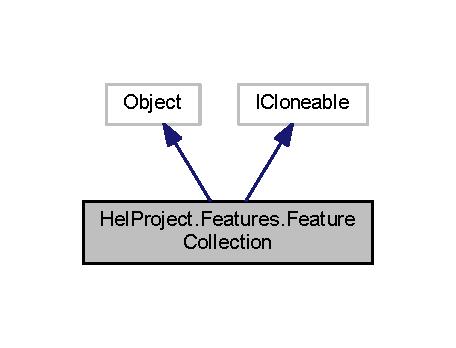
\includegraphics[width=219pt]{class_hel_project_1_1_features_1_1_feature_collection__inherit__graph}
\end{center}
\end{figure}


Collaboration diagram for Hel\+Project.\+Features.\+Feature\+Collection\+:\nopagebreak
\begin{figure}[H]
\begin{center}
\leavevmode
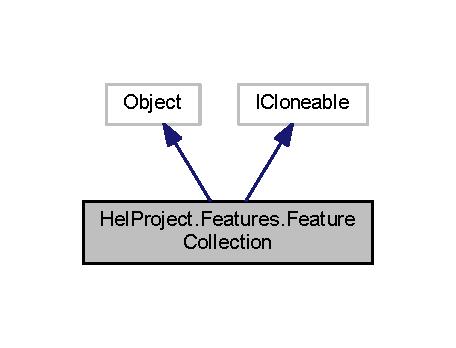
\includegraphics[width=219pt]{class_hel_project_1_1_features_1_1_feature_collection__coll__graph}
\end{center}
\end{figure}
\subsection*{Public Member Functions}
\begin{DoxyCompactItemize}
\item 
\hyperlink{class_hel_project_1_1_features_1_1_feature_collection_a8494a00531f9807cb6e5c57137a12ee8}{Feature\+Collection} ()
\begin{DoxyCompactList}\small\item\em Creates a feature collection \end{DoxyCompactList}\item 
object \hyperlink{class_hel_project_1_1_features_1_1_feature_collection_a920d45565d353cc73c05055018d498eb}{Clone} ()
\begin{DoxyCompactList}\small\item\em Clones the object \end{DoxyCompactList}\end{DoxyCompactItemize}
\subsection*{Properties}
\begin{DoxyCompactItemize}
\item 
float \hyperlink{class_hel_project_1_1_features_1_1_feature_collection_a4c9536777b3c49fe8804f04af8d334fd}{Initial\+Life\+Points}\hspace{0.3cm}{\ttfamily  \mbox{[}get, set\mbox{]}}
\begin{DoxyCompactList}\small\item\em Imposed life points \end{DoxyCompactList}\item 
float \hyperlink{class_hel_project_1_1_features_1_1_feature_collection_aaec4f751de75d95d240fa22e8826dde7}{Initial\+Attack\+Speed}\hspace{0.3cm}{\ttfamily  \mbox{[}get, set\mbox{]}}
\begin{DoxyCompactList}\small\item\em Imposed attack speed (attacks per second) \end{DoxyCompactList}\item 
float \hyperlink{class_hel_project_1_1_features_1_1_feature_collection_a9895c940500d9d028278ea3c175fd916}{Initial\+Movement\+Speed}\hspace{0.3cm}{\ttfamily  \mbox{[}get, set\mbox{]}}
\begin{DoxyCompactList}\small\item\em Imposed movement speed (meters / second) \end{DoxyCompactList}\item 
float \hyperlink{class_hel_project_1_1_features_1_1_feature_collection_a83624876566cbf6cf24e9f566bbd701e}{Initial\+Mana\+Regeneration}\hspace{0.3cm}{\ttfamily  \mbox{[}get, set\mbox{]}}
\begin{DoxyCompactList}\small\item\em Imposed mana regeneration (mana per second) \end{DoxyCompactList}\item 
float \hyperlink{class_hel_project_1_1_features_1_1_feature_collection_a69632e8a405d871ac827107ddb4b24f3}{Strenght}\hspace{0.3cm}{\ttfamily  \mbox{[}get, set\mbox{]}}
\begin{DoxyCompactList}\small\item\em Strenght points \end{DoxyCompactList}\item 
float \hyperlink{class_hel_project_1_1_features_1_1_feature_collection_a6254f82bffd41e3ca3beacf1928bb409}{Agility}\hspace{0.3cm}{\ttfamily  \mbox{[}get, set\mbox{]}}
\begin{DoxyCompactList}\small\item\em Agility points \end{DoxyCompactList}\item 
float \hyperlink{class_hel_project_1_1_features_1_1_feature_collection_a27719b073c6acce4f5faba5a437e1a70}{Vitality}\hspace{0.3cm}{\ttfamily  \mbox{[}get, set\mbox{]}}
\begin{DoxyCompactList}\small\item\em Vitality points \end{DoxyCompactList}\item 
float \hyperlink{class_hel_project_1_1_features_1_1_feature_collection_a7e5d56ee0fb50efbc2078002c01ff704}{Magic}\hspace{0.3cm}{\ttfamily  \mbox{[}get, set\mbox{]}}
\begin{DoxyCompactList}\small\item\em Magic points \end{DoxyCompactList}\item 
float \hyperlink{class_hel_project_1_1_features_1_1_feature_collection_a0e3d5ed05e9d748eaa03e861ca0c6470}{Attack\+Speed}\hspace{0.3cm}{\ttfamily  \mbox{[}get, set\mbox{]}}
\begin{DoxyCompactList}\small\item\em Attack speed buff percentage \end{DoxyCompactList}\item 
float \hyperlink{class_hel_project_1_1_features_1_1_feature_collection_ab8e635daa04259ac6ac50f1c78133fc2}{Minimum\+Damage}\hspace{0.3cm}{\ttfamily  \mbox{[}get, set\mbox{]}}
\begin{DoxyCompactList}\small\item\em Minimum damage \end{DoxyCompactList}\item 
float \hyperlink{class_hel_project_1_1_features_1_1_feature_collection_aeb58ea21cbca8600e2a4a65ab0399d0d}{Maximum\+Damage}\hspace{0.3cm}{\ttfamily  \mbox{[}get, set\mbox{]}}
\begin{DoxyCompactList}\small\item\em Maximum damage \end{DoxyCompactList}\item 
float \hyperlink{class_hel_project_1_1_features_1_1_feature_collection_a63883eb7a9cf40645502d92e722e7bf3}{Minimum\+Magic\+Damage}\hspace{0.3cm}{\ttfamily  \mbox{[}get, set\mbox{]}}
\begin{DoxyCompactList}\small\item\em Minimum magic damage \end{DoxyCompactList}\item 
float \hyperlink{class_hel_project_1_1_features_1_1_feature_collection_a231d947a27b442bfedb8b768e62b0984}{Maximum\+Magic\+Damage}\hspace{0.3cm}{\ttfamily  \mbox{[}get, set\mbox{]}}
\begin{DoxyCompactList}\small\item\em Maximum magic damage \end{DoxyCompactList}\item 
float \hyperlink{class_hel_project_1_1_features_1_1_feature_collection_a5485b8d9e8d3f4773c4599c66c22c11c}{Armor}\hspace{0.3cm}{\ttfamily  \mbox{[}get, set\mbox{]}}
\begin{DoxyCompactList}\small\item\em Armor points \end{DoxyCompactList}\item 
float \hyperlink{class_hel_project_1_1_features_1_1_feature_collection_a75958bd28bcc931507fe4186a8fa93f0}{Magic\+Resistance}\hspace{0.3cm}{\ttfamily  \mbox{[}get, set\mbox{]}}
\begin{DoxyCompactList}\small\item\em Magic resistance points \end{DoxyCompactList}\item 
float \hyperlink{class_hel_project_1_1_features_1_1_feature_collection_a8be9097e1627878b3a2d9719e07bf4bc}{Life\+Regeneration}\hspace{0.3cm}{\ttfamily  \mbox{[}get, set\mbox{]}}
\begin{DoxyCompactList}\small\item\em Life regeneration (life per second) \end{DoxyCompactList}\item 
float \hyperlink{class_hel_project_1_1_features_1_1_feature_collection_a1fca3d022c8171a1d0f20364cac6ba8a}{Mana\+Regeneration}\hspace{0.3cm}{\ttfamily  \mbox{[}get, set\mbox{]}}
\begin{DoxyCompactList}\small\item\em Mana regeneration (mana per second) \end{DoxyCompactList}\item 
float \hyperlink{class_hel_project_1_1_features_1_1_feature_collection_a8a35e6743d1291c75dc442f6464c5769}{Movement\+Speed}\hspace{0.3cm}{\ttfamily  \mbox{[}get, set\mbox{]}}
\begin{DoxyCompactList}\small\item\em Movement speed buff (percentage) \end{DoxyCompactList}\item 
float \hyperlink{class_hel_project_1_1_features_1_1_feature_collection_aa5b4b80b733386bb7bfb742b8481f4e8}{Life\+Points}\hspace{0.3cm}{\ttfamily  \mbox{[}get, set\mbox{]}}
\begin{DoxyCompactList}\small\item\em Life points \end{DoxyCompactList}\end{DoxyCompactItemize}


\subsection{Constructor \& Destructor Documentation}
\hypertarget{class_hel_project_1_1_features_1_1_feature_collection_a8494a00531f9807cb6e5c57137a12ee8}{}\index{Hel\+Project\+::\+Features\+::\+Feature\+Collection@{Hel\+Project\+::\+Features\+::\+Feature\+Collection}!Feature\+Collection@{Feature\+Collection}}
\index{Feature\+Collection@{Feature\+Collection}!Hel\+Project\+::\+Features\+::\+Feature\+Collection@{Hel\+Project\+::\+Features\+::\+Feature\+Collection}}
\subsubsection[{Feature\+Collection}]{\setlength{\rightskip}{0pt plus 5cm}Hel\+Project.\+Features.\+Feature\+Collection.\+Feature\+Collection (
\begin{DoxyParamCaption}
{}
\end{DoxyParamCaption}
)}\label{class_hel_project_1_1_features_1_1_feature_collection_a8494a00531f9807cb6e5c57137a12ee8}


Creates a feature collection 



\subsection{Member Function Documentation}
\hypertarget{class_hel_project_1_1_features_1_1_feature_collection_a920d45565d353cc73c05055018d498eb}{}\index{Hel\+Project\+::\+Features\+::\+Feature\+Collection@{Hel\+Project\+::\+Features\+::\+Feature\+Collection}!Clone@{Clone}}
\index{Clone@{Clone}!Hel\+Project\+::\+Features\+::\+Feature\+Collection@{Hel\+Project\+::\+Features\+::\+Feature\+Collection}}
\subsubsection[{Clone}]{\setlength{\rightskip}{0pt plus 5cm}object Hel\+Project.\+Features.\+Feature\+Collection.\+Clone (
\begin{DoxyParamCaption}
{}
\end{DoxyParamCaption}
)}\label{class_hel_project_1_1_features_1_1_feature_collection_a920d45565d353cc73c05055018d498eb}


Clones the object 

\begin{DoxyReturn}{Returns}
object
\end{DoxyReturn}


\subsection{Property Documentation}
\hypertarget{class_hel_project_1_1_features_1_1_feature_collection_a6254f82bffd41e3ca3beacf1928bb409}{}\index{Hel\+Project\+::\+Features\+::\+Feature\+Collection@{Hel\+Project\+::\+Features\+::\+Feature\+Collection}!Agility@{Agility}}
\index{Agility@{Agility}!Hel\+Project\+::\+Features\+::\+Feature\+Collection@{Hel\+Project\+::\+Features\+::\+Feature\+Collection}}
\subsubsection[{Agility}]{\setlength{\rightskip}{0pt plus 5cm}float Hel\+Project.\+Features.\+Feature\+Collection.\+Agility\hspace{0.3cm}{\ttfamily [get]}, {\ttfamily [set]}}\label{class_hel_project_1_1_features_1_1_feature_collection_a6254f82bffd41e3ca3beacf1928bb409}


Agility points 

\hypertarget{class_hel_project_1_1_features_1_1_feature_collection_a5485b8d9e8d3f4773c4599c66c22c11c}{}\index{Hel\+Project\+::\+Features\+::\+Feature\+Collection@{Hel\+Project\+::\+Features\+::\+Feature\+Collection}!Armor@{Armor}}
\index{Armor@{Armor}!Hel\+Project\+::\+Features\+::\+Feature\+Collection@{Hel\+Project\+::\+Features\+::\+Feature\+Collection}}
\subsubsection[{Armor}]{\setlength{\rightskip}{0pt plus 5cm}float Hel\+Project.\+Features.\+Feature\+Collection.\+Armor\hspace{0.3cm}{\ttfamily [get]}, {\ttfamily [set]}}\label{class_hel_project_1_1_features_1_1_feature_collection_a5485b8d9e8d3f4773c4599c66c22c11c}


Armor points 

\hypertarget{class_hel_project_1_1_features_1_1_feature_collection_a0e3d5ed05e9d748eaa03e861ca0c6470}{}\index{Hel\+Project\+::\+Features\+::\+Feature\+Collection@{Hel\+Project\+::\+Features\+::\+Feature\+Collection}!Attack\+Speed@{Attack\+Speed}}
\index{Attack\+Speed@{Attack\+Speed}!Hel\+Project\+::\+Features\+::\+Feature\+Collection@{Hel\+Project\+::\+Features\+::\+Feature\+Collection}}
\subsubsection[{Attack\+Speed}]{\setlength{\rightskip}{0pt plus 5cm}float Hel\+Project.\+Features.\+Feature\+Collection.\+Attack\+Speed\hspace{0.3cm}{\ttfamily [get]}, {\ttfamily [set]}}\label{class_hel_project_1_1_features_1_1_feature_collection_a0e3d5ed05e9d748eaa03e861ca0c6470}


Attack speed buff percentage 

25\%\hypertarget{class_hel_project_1_1_features_1_1_feature_collection_aaec4f751de75d95d240fa22e8826dde7}{}\index{Hel\+Project\+::\+Features\+::\+Feature\+Collection@{Hel\+Project\+::\+Features\+::\+Feature\+Collection}!Initial\+Attack\+Speed@{Initial\+Attack\+Speed}}
\index{Initial\+Attack\+Speed@{Initial\+Attack\+Speed}!Hel\+Project\+::\+Features\+::\+Feature\+Collection@{Hel\+Project\+::\+Features\+::\+Feature\+Collection}}
\subsubsection[{Initial\+Attack\+Speed}]{\setlength{\rightskip}{0pt plus 5cm}float Hel\+Project.\+Features.\+Feature\+Collection.\+Initial\+Attack\+Speed\hspace{0.3cm}{\ttfamily [get]}, {\ttfamily [set]}}\label{class_hel_project_1_1_features_1_1_feature_collection_aaec4f751de75d95d240fa22e8826dde7}


Imposed attack speed (attacks per second) 

\hypertarget{class_hel_project_1_1_features_1_1_feature_collection_a4c9536777b3c49fe8804f04af8d334fd}{}\index{Hel\+Project\+::\+Features\+::\+Feature\+Collection@{Hel\+Project\+::\+Features\+::\+Feature\+Collection}!Initial\+Life\+Points@{Initial\+Life\+Points}}
\index{Initial\+Life\+Points@{Initial\+Life\+Points}!Hel\+Project\+::\+Features\+::\+Feature\+Collection@{Hel\+Project\+::\+Features\+::\+Feature\+Collection}}
\subsubsection[{Initial\+Life\+Points}]{\setlength{\rightskip}{0pt plus 5cm}float Hel\+Project.\+Features.\+Feature\+Collection.\+Initial\+Life\+Points\hspace{0.3cm}{\ttfamily [get]}, {\ttfamily [set]}}\label{class_hel_project_1_1_features_1_1_feature_collection_a4c9536777b3c49fe8804f04af8d334fd}


Imposed life points 

\hypertarget{class_hel_project_1_1_features_1_1_feature_collection_a83624876566cbf6cf24e9f566bbd701e}{}\index{Hel\+Project\+::\+Features\+::\+Feature\+Collection@{Hel\+Project\+::\+Features\+::\+Feature\+Collection}!Initial\+Mana\+Regeneration@{Initial\+Mana\+Regeneration}}
\index{Initial\+Mana\+Regeneration@{Initial\+Mana\+Regeneration}!Hel\+Project\+::\+Features\+::\+Feature\+Collection@{Hel\+Project\+::\+Features\+::\+Feature\+Collection}}
\subsubsection[{Initial\+Mana\+Regeneration}]{\setlength{\rightskip}{0pt plus 5cm}float Hel\+Project.\+Features.\+Feature\+Collection.\+Initial\+Mana\+Regeneration\hspace{0.3cm}{\ttfamily [get]}, {\ttfamily [set]}}\label{class_hel_project_1_1_features_1_1_feature_collection_a83624876566cbf6cf24e9f566bbd701e}


Imposed mana regeneration (mana per second) 

\hypertarget{class_hel_project_1_1_features_1_1_feature_collection_a9895c940500d9d028278ea3c175fd916}{}\index{Hel\+Project\+::\+Features\+::\+Feature\+Collection@{Hel\+Project\+::\+Features\+::\+Feature\+Collection}!Initial\+Movement\+Speed@{Initial\+Movement\+Speed}}
\index{Initial\+Movement\+Speed@{Initial\+Movement\+Speed}!Hel\+Project\+::\+Features\+::\+Feature\+Collection@{Hel\+Project\+::\+Features\+::\+Feature\+Collection}}
\subsubsection[{Initial\+Movement\+Speed}]{\setlength{\rightskip}{0pt plus 5cm}float Hel\+Project.\+Features.\+Feature\+Collection.\+Initial\+Movement\+Speed\hspace{0.3cm}{\ttfamily [get]}, {\ttfamily [set]}}\label{class_hel_project_1_1_features_1_1_feature_collection_a9895c940500d9d028278ea3c175fd916}


Imposed movement speed (meters / second) 

\hypertarget{class_hel_project_1_1_features_1_1_feature_collection_aa5b4b80b733386bb7bfb742b8481f4e8}{}\index{Hel\+Project\+::\+Features\+::\+Feature\+Collection@{Hel\+Project\+::\+Features\+::\+Feature\+Collection}!Life\+Points@{Life\+Points}}
\index{Life\+Points@{Life\+Points}!Hel\+Project\+::\+Features\+::\+Feature\+Collection@{Hel\+Project\+::\+Features\+::\+Feature\+Collection}}
\subsubsection[{Life\+Points}]{\setlength{\rightskip}{0pt plus 5cm}float Hel\+Project.\+Features.\+Feature\+Collection.\+Life\+Points\hspace{0.3cm}{\ttfamily [get]}, {\ttfamily [set]}}\label{class_hel_project_1_1_features_1_1_feature_collection_aa5b4b80b733386bb7bfb742b8481f4e8}


Life points 

\hypertarget{class_hel_project_1_1_features_1_1_feature_collection_a8be9097e1627878b3a2d9719e07bf4bc}{}\index{Hel\+Project\+::\+Features\+::\+Feature\+Collection@{Hel\+Project\+::\+Features\+::\+Feature\+Collection}!Life\+Regeneration@{Life\+Regeneration}}
\index{Life\+Regeneration@{Life\+Regeneration}!Hel\+Project\+::\+Features\+::\+Feature\+Collection@{Hel\+Project\+::\+Features\+::\+Feature\+Collection}}
\subsubsection[{Life\+Regeneration}]{\setlength{\rightskip}{0pt plus 5cm}float Hel\+Project.\+Features.\+Feature\+Collection.\+Life\+Regeneration\hspace{0.3cm}{\ttfamily [get]}, {\ttfamily [set]}}\label{class_hel_project_1_1_features_1_1_feature_collection_a8be9097e1627878b3a2d9719e07bf4bc}


Life regeneration (life per second) 

\hypertarget{class_hel_project_1_1_features_1_1_feature_collection_a7e5d56ee0fb50efbc2078002c01ff704}{}\index{Hel\+Project\+::\+Features\+::\+Feature\+Collection@{Hel\+Project\+::\+Features\+::\+Feature\+Collection}!Magic@{Magic}}
\index{Magic@{Magic}!Hel\+Project\+::\+Features\+::\+Feature\+Collection@{Hel\+Project\+::\+Features\+::\+Feature\+Collection}}
\subsubsection[{Magic}]{\setlength{\rightskip}{0pt plus 5cm}float Hel\+Project.\+Features.\+Feature\+Collection.\+Magic\hspace{0.3cm}{\ttfamily [get]}, {\ttfamily [set]}}\label{class_hel_project_1_1_features_1_1_feature_collection_a7e5d56ee0fb50efbc2078002c01ff704}


Magic points 

\hypertarget{class_hel_project_1_1_features_1_1_feature_collection_a75958bd28bcc931507fe4186a8fa93f0}{}\index{Hel\+Project\+::\+Features\+::\+Feature\+Collection@{Hel\+Project\+::\+Features\+::\+Feature\+Collection}!Magic\+Resistance@{Magic\+Resistance}}
\index{Magic\+Resistance@{Magic\+Resistance}!Hel\+Project\+::\+Features\+::\+Feature\+Collection@{Hel\+Project\+::\+Features\+::\+Feature\+Collection}}
\subsubsection[{Magic\+Resistance}]{\setlength{\rightskip}{0pt plus 5cm}float Hel\+Project.\+Features.\+Feature\+Collection.\+Magic\+Resistance\hspace{0.3cm}{\ttfamily [get]}, {\ttfamily [set]}}\label{class_hel_project_1_1_features_1_1_feature_collection_a75958bd28bcc931507fe4186a8fa93f0}


Magic resistance points 

\hypertarget{class_hel_project_1_1_features_1_1_feature_collection_a1fca3d022c8171a1d0f20364cac6ba8a}{}\index{Hel\+Project\+::\+Features\+::\+Feature\+Collection@{Hel\+Project\+::\+Features\+::\+Feature\+Collection}!Mana\+Regeneration@{Mana\+Regeneration}}
\index{Mana\+Regeneration@{Mana\+Regeneration}!Hel\+Project\+::\+Features\+::\+Feature\+Collection@{Hel\+Project\+::\+Features\+::\+Feature\+Collection}}
\subsubsection[{Mana\+Regeneration}]{\setlength{\rightskip}{0pt plus 5cm}float Hel\+Project.\+Features.\+Feature\+Collection.\+Mana\+Regeneration\hspace{0.3cm}{\ttfamily [get]}, {\ttfamily [set]}}\label{class_hel_project_1_1_features_1_1_feature_collection_a1fca3d022c8171a1d0f20364cac6ba8a}


Mana regeneration (mana per second) 

\hypertarget{class_hel_project_1_1_features_1_1_feature_collection_aeb58ea21cbca8600e2a4a65ab0399d0d}{}\index{Hel\+Project\+::\+Features\+::\+Feature\+Collection@{Hel\+Project\+::\+Features\+::\+Feature\+Collection}!Maximum\+Damage@{Maximum\+Damage}}
\index{Maximum\+Damage@{Maximum\+Damage}!Hel\+Project\+::\+Features\+::\+Feature\+Collection@{Hel\+Project\+::\+Features\+::\+Feature\+Collection}}
\subsubsection[{Maximum\+Damage}]{\setlength{\rightskip}{0pt plus 5cm}float Hel\+Project.\+Features.\+Feature\+Collection.\+Maximum\+Damage\hspace{0.3cm}{\ttfamily [get]}, {\ttfamily [set]}}\label{class_hel_project_1_1_features_1_1_feature_collection_aeb58ea21cbca8600e2a4a65ab0399d0d}


Maximum damage 

\hypertarget{class_hel_project_1_1_features_1_1_feature_collection_a231d947a27b442bfedb8b768e62b0984}{}\index{Hel\+Project\+::\+Features\+::\+Feature\+Collection@{Hel\+Project\+::\+Features\+::\+Feature\+Collection}!Maximum\+Magic\+Damage@{Maximum\+Magic\+Damage}}
\index{Maximum\+Magic\+Damage@{Maximum\+Magic\+Damage}!Hel\+Project\+::\+Features\+::\+Feature\+Collection@{Hel\+Project\+::\+Features\+::\+Feature\+Collection}}
\subsubsection[{Maximum\+Magic\+Damage}]{\setlength{\rightskip}{0pt plus 5cm}float Hel\+Project.\+Features.\+Feature\+Collection.\+Maximum\+Magic\+Damage\hspace{0.3cm}{\ttfamily [get]}, {\ttfamily [set]}}\label{class_hel_project_1_1_features_1_1_feature_collection_a231d947a27b442bfedb8b768e62b0984}


Maximum magic damage 

\hypertarget{class_hel_project_1_1_features_1_1_feature_collection_ab8e635daa04259ac6ac50f1c78133fc2}{}\index{Hel\+Project\+::\+Features\+::\+Feature\+Collection@{Hel\+Project\+::\+Features\+::\+Feature\+Collection}!Minimum\+Damage@{Minimum\+Damage}}
\index{Minimum\+Damage@{Minimum\+Damage}!Hel\+Project\+::\+Features\+::\+Feature\+Collection@{Hel\+Project\+::\+Features\+::\+Feature\+Collection}}
\subsubsection[{Minimum\+Damage}]{\setlength{\rightskip}{0pt plus 5cm}float Hel\+Project.\+Features.\+Feature\+Collection.\+Minimum\+Damage\hspace{0.3cm}{\ttfamily [get]}, {\ttfamily [set]}}\label{class_hel_project_1_1_features_1_1_feature_collection_ab8e635daa04259ac6ac50f1c78133fc2}


Minimum damage 

\hypertarget{class_hel_project_1_1_features_1_1_feature_collection_a63883eb7a9cf40645502d92e722e7bf3}{}\index{Hel\+Project\+::\+Features\+::\+Feature\+Collection@{Hel\+Project\+::\+Features\+::\+Feature\+Collection}!Minimum\+Magic\+Damage@{Minimum\+Magic\+Damage}}
\index{Minimum\+Magic\+Damage@{Minimum\+Magic\+Damage}!Hel\+Project\+::\+Features\+::\+Feature\+Collection@{Hel\+Project\+::\+Features\+::\+Feature\+Collection}}
\subsubsection[{Minimum\+Magic\+Damage}]{\setlength{\rightskip}{0pt plus 5cm}float Hel\+Project.\+Features.\+Feature\+Collection.\+Minimum\+Magic\+Damage\hspace{0.3cm}{\ttfamily [get]}, {\ttfamily [set]}}\label{class_hel_project_1_1_features_1_1_feature_collection_a63883eb7a9cf40645502d92e722e7bf3}


Minimum magic damage 

\hypertarget{class_hel_project_1_1_features_1_1_feature_collection_a8a35e6743d1291c75dc442f6464c5769}{}\index{Hel\+Project\+::\+Features\+::\+Feature\+Collection@{Hel\+Project\+::\+Features\+::\+Feature\+Collection}!Movement\+Speed@{Movement\+Speed}}
\index{Movement\+Speed@{Movement\+Speed}!Hel\+Project\+::\+Features\+::\+Feature\+Collection@{Hel\+Project\+::\+Features\+::\+Feature\+Collection}}
\subsubsection[{Movement\+Speed}]{\setlength{\rightskip}{0pt plus 5cm}float Hel\+Project.\+Features.\+Feature\+Collection.\+Movement\+Speed\hspace{0.3cm}{\ttfamily [get]}, {\ttfamily [set]}}\label{class_hel_project_1_1_features_1_1_feature_collection_a8a35e6743d1291c75dc442f6464c5769}


Movement speed buff (percentage) 

25\%\hypertarget{class_hel_project_1_1_features_1_1_feature_collection_a69632e8a405d871ac827107ddb4b24f3}{}\index{Hel\+Project\+::\+Features\+::\+Feature\+Collection@{Hel\+Project\+::\+Features\+::\+Feature\+Collection}!Strenght@{Strenght}}
\index{Strenght@{Strenght}!Hel\+Project\+::\+Features\+::\+Feature\+Collection@{Hel\+Project\+::\+Features\+::\+Feature\+Collection}}
\subsubsection[{Strenght}]{\setlength{\rightskip}{0pt plus 5cm}float Hel\+Project.\+Features.\+Feature\+Collection.\+Strenght\hspace{0.3cm}{\ttfamily [get]}, {\ttfamily [set]}}\label{class_hel_project_1_1_features_1_1_feature_collection_a69632e8a405d871ac827107ddb4b24f3}


Strenght points 

\hypertarget{class_hel_project_1_1_features_1_1_feature_collection_a27719b073c6acce4f5faba5a437e1a70}{}\index{Hel\+Project\+::\+Features\+::\+Feature\+Collection@{Hel\+Project\+::\+Features\+::\+Feature\+Collection}!Vitality@{Vitality}}
\index{Vitality@{Vitality}!Hel\+Project\+::\+Features\+::\+Feature\+Collection@{Hel\+Project\+::\+Features\+::\+Feature\+Collection}}
\subsubsection[{Vitality}]{\setlength{\rightskip}{0pt plus 5cm}float Hel\+Project.\+Features.\+Feature\+Collection.\+Vitality\hspace{0.3cm}{\ttfamily [get]}, {\ttfamily [set]}}\label{class_hel_project_1_1_features_1_1_feature_collection_a27719b073c6acce4f5faba5a437e1a70}


Vitality points 



The documentation for this class was generated from the following file\+:\begin{DoxyCompactItemize}
\item 
src/\+Hel\+Project/\+Features/Feature\+Collection.\+cs\end{DoxyCompactItemize}

\hypertarget{class_hel_project_1_1_features_1_1_feature_manager}{}\section{Hel\+Project.\+Features.\+Feature\+Manager Class Reference}
\label{class_hel_project_1_1_features_1_1_feature_manager}\index{Hel\+Project.\+Features.\+Feature\+Manager@{Hel\+Project.\+Features.\+Feature\+Manager}}


Manages the calculation of the feature for the entities  


\subsection*{Public Member Functions}
\begin{DoxyCompactItemize}
\item 
\hyperlink{class_hel_project_1_1_features_1_1_feature_manager_aa0f53d0bac56de1cdb4fb36c0d56708b}{Feature\+Manager} (\hyperlink{class_hel_project_1_1_features_1_1_feature_collection}{Feature\+Collection} features, List$<$ \hyperlink{class_hel_project_1_1_game_world_1_1_spells_1_1_h_spell}{H\+Spell} $>$ spells=null, List$<$ \hyperlink{class_hel_project_1_1_game_world_1_1_h_item}{H\+Item} $>$ items=null)
\begin{DoxyCompactList}\small\item\em Creates a feature manager \end{DoxyCompactList}\item 
\hyperlink{class_hel_project_1_1_features_1_1_feature_collection}{Feature\+Collection} \hyperlink{class_hel_project_1_1_features_1_1_feature_manager_aaa192e040c25fefa91e5d6abd99625c0}{Get\+Calculated\+Features} ()
\begin{DoxyCompactList}\small\item\em Gets the calculated features \end{DoxyCompactList}\item 
float \hyperlink{class_hel_project_1_1_features_1_1_feature_manager_a84f16b535f2140f2255202deaab08db6}{Get\+Total\+Strenght} ()
\begin{DoxyCompactList}\small\item\em Calculates the total strenght within the items, spells and initial values \end{DoxyCompactList}\item 
float \hyperlink{class_hel_project_1_1_features_1_1_feature_manager_ac90f3988658e1b3976e75e430bb6e4c5}{Get\+Total\+Agility} ()
\begin{DoxyCompactList}\small\item\em Calculates the total agility within the items, spells and initial values \end{DoxyCompactList}\item 
float \hyperlink{class_hel_project_1_1_features_1_1_feature_manager_adcdbe81d240dd214000ca6a1bc46f9b1}{Get\+Total\+Vitality} ()
\begin{DoxyCompactList}\small\item\em Calculates the total Vitality within the items, spells and initial values \end{DoxyCompactList}\item 
float \hyperlink{class_hel_project_1_1_features_1_1_feature_manager_a8795128921c9d40161ea2cc54f0cd558}{Get\+Total\+Magic} ()
\begin{DoxyCompactList}\small\item\em Calculates the total Magic within the items, spells and initial values \end{DoxyCompactList}\item 
float \hyperlink{class_hel_project_1_1_features_1_1_feature_manager_a180a0742fc037b731348d82b960bd007}{Get\+Total\+Attack\+Speed} ()
\begin{DoxyCompactList}\small\item\em Calculates the total Attack\+Speed within the items, spells and initial values \end{DoxyCompactList}\item 
float \hyperlink{class_hel_project_1_1_features_1_1_feature_manager_a70cd5fd60ddb0d35810f4e8f55fdeadc}{Get\+Total\+Minimum\+Damage} ()
\begin{DoxyCompactList}\small\item\em Calculates the total Minimum\+Damage within the items, spells and initial values \end{DoxyCompactList}\item 
float \hyperlink{class_hel_project_1_1_features_1_1_feature_manager_aa2a965173213b11c08f3b25f5c920ccb}{Get\+Total\+Maximum\+Damage} ()
\begin{DoxyCompactList}\small\item\em Calculates the total Maximum\+Damage within the items, spells and initial values \end{DoxyCompactList}\item 
float \hyperlink{class_hel_project_1_1_features_1_1_feature_manager_aca527aecc8a8ea7370bc279e3237279b}{Get\+Total\+Minimum\+Magic\+Damage} ()
\begin{DoxyCompactList}\small\item\em Calculates the total Minimum\+Magic\+Damage within the items, spells and initial values \end{DoxyCompactList}\item 
float \hyperlink{class_hel_project_1_1_features_1_1_feature_manager_a53a153e4dae0b823c34e4546968d927e}{Get\+Total\+Maximum\+Magic\+Damage} ()
\begin{DoxyCompactList}\small\item\em Calculates the total Maximum\+Magic\+Damage within the items, spells and initial values \end{DoxyCompactList}\item 
float \hyperlink{class_hel_project_1_1_features_1_1_feature_manager_aeae79cbc3c27d4fd9796269a26e3d349}{Get\+Total\+Armor} ()
\begin{DoxyCompactList}\small\item\em Calculates the total Armor within the items, spells and initial values \end{DoxyCompactList}\item 
float \hyperlink{class_hel_project_1_1_features_1_1_feature_manager_aa00b054d0ce926e2a1c0839364a55a81}{Get\+Total\+Magic\+Resistance} ()
\begin{DoxyCompactList}\small\item\em Calculates the total Magic\+Resistance within the items, spells and initial values \end{DoxyCompactList}\item 
float \hyperlink{class_hel_project_1_1_features_1_1_feature_manager_ae58d9838038b0589739863d3aefc5e9a}{Get\+Total\+Life\+Regeneration} ()
\begin{DoxyCompactList}\small\item\em Calculates the total Life\+Regeneration within the items, spells and initial values \end{DoxyCompactList}\item 
float \hyperlink{class_hel_project_1_1_features_1_1_feature_manager_a63c2d856a598a7d37c2f305e066db1d5}{Get\+Total\+Mana\+Regeneration} ()
\begin{DoxyCompactList}\small\item\em Calculates the total Mana\+Regeneration within the items, spells and initial values \end{DoxyCompactList}\item 
float \hyperlink{class_hel_project_1_1_features_1_1_feature_manager_a41763411f2016d354b8f281ea26ea79f}{Get\+Total\+Movement\+Speed} ()
\begin{DoxyCompactList}\small\item\em Calculates the total Movement\+Speed within the items, spells and initial values \end{DoxyCompactList}\item 
float \hyperlink{class_hel_project_1_1_features_1_1_feature_manager_a226f7b884b8de2556e8b12fec879d927}{Get\+Total\+Life\+Points} ()
\begin{DoxyCompactList}\small\item\em Calculates the total Life\+Points within the items, spells and initial values \end{DoxyCompactList}\end{DoxyCompactItemize}
\subsection*{Public Attributes}
\begin{DoxyCompactItemize}
\item 
\hypertarget{class_hel_project_1_1_features_1_1_feature_manager_a82ddccda10f8361c1ba5b386037a427e}{}const float {\bfseries L\+I\+F\+E\+\_\+\+P\+E\+R\+\_\+\+V\+I\+T\+A\+L\+I\+T\+Y} = 100.\+0f\label{class_hel_project_1_1_features_1_1_feature_manager_a82ddccda10f8361c1ba5b386037a427e}

\end{DoxyCompactItemize}
\subsection*{Properties}
\begin{DoxyCompactItemize}
\item 
List$<$ \hyperlink{class_hel_project_1_1_game_world_1_1_h_item}{H\+Item} $>$ \hyperlink{class_hel_project_1_1_features_1_1_feature_manager_a12a4a1dfd4a78d9cd47ae79b6bc6b7da}{Active\+Items}\hspace{0.3cm}{\ttfamily  \mbox{[}get, set\mbox{]}}
\begin{DoxyCompactList}\small\item\em Items worn by the hero \end{DoxyCompactList}\item 
List$<$ \hyperlink{class_hel_project_1_1_game_world_1_1_spells_1_1_h_spell}{H\+Spell} $>$ \hyperlink{class_hel_project_1_1_features_1_1_feature_manager_afc065fffad775f30c796536009f67e24}{Active\+Spells}\hspace{0.3cm}{\ttfamily  \mbox{[}get, set\mbox{]}}
\begin{DoxyCompactList}\small\item\em Currently casted spells of the hero \end{DoxyCompactList}\item 
\hyperlink{class_hel_project_1_1_features_1_1_feature_collection}{Feature\+Collection} \hyperlink{class_hel_project_1_1_features_1_1_feature_manager_a11ca4dbbba29012ad2633728518e5dd7}{Initial\+Features}\hspace{0.3cm}{\ttfamily  \mbox{[}get, set\mbox{]}}
\begin{DoxyCompactList}\small\item\em Initial features of the hero \end{DoxyCompactList}\end{DoxyCompactItemize}


\subsection{Detailed Description}
Manages the calculation of the feature for the entities 



\subsection{Constructor \& Destructor Documentation}
\hypertarget{class_hel_project_1_1_features_1_1_feature_manager_aa0f53d0bac56de1cdb4fb36c0d56708b}{}\index{Hel\+Project\+::\+Features\+::\+Feature\+Manager@{Hel\+Project\+::\+Features\+::\+Feature\+Manager}!Feature\+Manager@{Feature\+Manager}}
\index{Feature\+Manager@{Feature\+Manager}!Hel\+Project\+::\+Features\+::\+Feature\+Manager@{Hel\+Project\+::\+Features\+::\+Feature\+Manager}}
\subsubsection[{Feature\+Manager}]{\setlength{\rightskip}{0pt plus 5cm}Hel\+Project.\+Features.\+Feature\+Manager.\+Feature\+Manager (
\begin{DoxyParamCaption}
\item[{{\bf Feature\+Collection}}]{features, }
\item[{List$<$ {\bf H\+Spell} $>$}]{spells = {\ttfamily null}, }
\item[{List$<$ {\bf H\+Item} $>$}]{items = {\ttfamily null}}
\end{DoxyParamCaption}
)}\label{class_hel_project_1_1_features_1_1_feature_manager_aa0f53d0bac56de1cdb4fb36c0d56708b}


Creates a feature manager 


\begin{DoxyParams}{Parameters}
{\em features} & Initial features of the hero\\
\hline
{\em spells} & Active spells of the hero\\
\hline
{\em items} & Worn items of the hero\\
\hline
\end{DoxyParams}


Null values will be initialized (except the \char`\"{}features\char`\"{} parameter).

\subsection{Member Function Documentation}
\hypertarget{class_hel_project_1_1_features_1_1_feature_manager_aaa192e040c25fefa91e5d6abd99625c0}{}\index{Hel\+Project\+::\+Features\+::\+Feature\+Manager@{Hel\+Project\+::\+Features\+::\+Feature\+Manager}!Get\+Calculated\+Features@{Get\+Calculated\+Features}}
\index{Get\+Calculated\+Features@{Get\+Calculated\+Features}!Hel\+Project\+::\+Features\+::\+Feature\+Manager@{Hel\+Project\+::\+Features\+::\+Feature\+Manager}}
\subsubsection[{Get\+Calculated\+Features}]{\setlength{\rightskip}{0pt plus 5cm}{\bf Feature\+Collection} Hel\+Project.\+Features.\+Feature\+Manager.\+Get\+Calculated\+Features (
\begin{DoxyParamCaption}
{}
\end{DoxyParamCaption}
)}\label{class_hel_project_1_1_features_1_1_feature_manager_aaa192e040c25fefa91e5d6abd99625c0}


Gets the calculated features 

\begin{DoxyReturn}{Returns}
Feature collection
\end{DoxyReturn}


For movement speed, use the initial movement speed\hypertarget{class_hel_project_1_1_features_1_1_feature_manager_ac90f3988658e1b3976e75e430bb6e4c5}{}\index{Hel\+Project\+::\+Features\+::\+Feature\+Manager@{Hel\+Project\+::\+Features\+::\+Feature\+Manager}!Get\+Total\+Agility@{Get\+Total\+Agility}}
\index{Get\+Total\+Agility@{Get\+Total\+Agility}!Hel\+Project\+::\+Features\+::\+Feature\+Manager@{Hel\+Project\+::\+Features\+::\+Feature\+Manager}}
\subsubsection[{Get\+Total\+Agility}]{\setlength{\rightskip}{0pt plus 5cm}float Hel\+Project.\+Features.\+Feature\+Manager.\+Get\+Total\+Agility (
\begin{DoxyParamCaption}
{}
\end{DoxyParamCaption}
)}\label{class_hel_project_1_1_features_1_1_feature_manager_ac90f3988658e1b3976e75e430bb6e4c5}


Calculates the total agility within the items, spells and initial values 

\begin{DoxyReturn}{Returns}
Total agility
\end{DoxyReturn}
\hypertarget{class_hel_project_1_1_features_1_1_feature_manager_aeae79cbc3c27d4fd9796269a26e3d349}{}\index{Hel\+Project\+::\+Features\+::\+Feature\+Manager@{Hel\+Project\+::\+Features\+::\+Feature\+Manager}!Get\+Total\+Armor@{Get\+Total\+Armor}}
\index{Get\+Total\+Armor@{Get\+Total\+Armor}!Hel\+Project\+::\+Features\+::\+Feature\+Manager@{Hel\+Project\+::\+Features\+::\+Feature\+Manager}}
\subsubsection[{Get\+Total\+Armor}]{\setlength{\rightskip}{0pt plus 5cm}float Hel\+Project.\+Features.\+Feature\+Manager.\+Get\+Total\+Armor (
\begin{DoxyParamCaption}
{}
\end{DoxyParamCaption}
)}\label{class_hel_project_1_1_features_1_1_feature_manager_aeae79cbc3c27d4fd9796269a26e3d349}


Calculates the total Armor within the items, spells and initial values 

\begin{DoxyReturn}{Returns}
Total Armor
\end{DoxyReturn}
\hypertarget{class_hel_project_1_1_features_1_1_feature_manager_a180a0742fc037b731348d82b960bd007}{}\index{Hel\+Project\+::\+Features\+::\+Feature\+Manager@{Hel\+Project\+::\+Features\+::\+Feature\+Manager}!Get\+Total\+Attack\+Speed@{Get\+Total\+Attack\+Speed}}
\index{Get\+Total\+Attack\+Speed@{Get\+Total\+Attack\+Speed}!Hel\+Project\+::\+Features\+::\+Feature\+Manager@{Hel\+Project\+::\+Features\+::\+Feature\+Manager}}
\subsubsection[{Get\+Total\+Attack\+Speed}]{\setlength{\rightskip}{0pt plus 5cm}float Hel\+Project.\+Features.\+Feature\+Manager.\+Get\+Total\+Attack\+Speed (
\begin{DoxyParamCaption}
{}
\end{DoxyParamCaption}
)}\label{class_hel_project_1_1_features_1_1_feature_manager_a180a0742fc037b731348d82b960bd007}


Calculates the total Attack\+Speed within the items, spells and initial values 

\begin{DoxyReturn}{Returns}
Total Attack\+Speed
\end{DoxyReturn}


Gets the highest initial attack speed and adds all the attack speed percentages\hypertarget{class_hel_project_1_1_features_1_1_feature_manager_a226f7b884b8de2556e8b12fec879d927}{}\index{Hel\+Project\+::\+Features\+::\+Feature\+Manager@{Hel\+Project\+::\+Features\+::\+Feature\+Manager}!Get\+Total\+Life\+Points@{Get\+Total\+Life\+Points}}
\index{Get\+Total\+Life\+Points@{Get\+Total\+Life\+Points}!Hel\+Project\+::\+Features\+::\+Feature\+Manager@{Hel\+Project\+::\+Features\+::\+Feature\+Manager}}
\subsubsection[{Get\+Total\+Life\+Points}]{\setlength{\rightskip}{0pt plus 5cm}float Hel\+Project.\+Features.\+Feature\+Manager.\+Get\+Total\+Life\+Points (
\begin{DoxyParamCaption}
{}
\end{DoxyParamCaption}
)}\label{class_hel_project_1_1_features_1_1_feature_manager_a226f7b884b8de2556e8b12fec879d927}


Calculates the total Life\+Points within the items, spells and initial values 

\begin{DoxyReturn}{Returns}
Total Life\+Points
\end{DoxyReturn}
\hypertarget{class_hel_project_1_1_features_1_1_feature_manager_ae58d9838038b0589739863d3aefc5e9a}{}\index{Hel\+Project\+::\+Features\+::\+Feature\+Manager@{Hel\+Project\+::\+Features\+::\+Feature\+Manager}!Get\+Total\+Life\+Regeneration@{Get\+Total\+Life\+Regeneration}}
\index{Get\+Total\+Life\+Regeneration@{Get\+Total\+Life\+Regeneration}!Hel\+Project\+::\+Features\+::\+Feature\+Manager@{Hel\+Project\+::\+Features\+::\+Feature\+Manager}}
\subsubsection[{Get\+Total\+Life\+Regeneration}]{\setlength{\rightskip}{0pt plus 5cm}float Hel\+Project.\+Features.\+Feature\+Manager.\+Get\+Total\+Life\+Regeneration (
\begin{DoxyParamCaption}
{}
\end{DoxyParamCaption}
)}\label{class_hel_project_1_1_features_1_1_feature_manager_ae58d9838038b0589739863d3aefc5e9a}


Calculates the total Life\+Regeneration within the items, spells and initial values 

\begin{DoxyReturn}{Returns}
Total Life\+Regeneration
\end{DoxyReturn}
\hypertarget{class_hel_project_1_1_features_1_1_feature_manager_a8795128921c9d40161ea2cc54f0cd558}{}\index{Hel\+Project\+::\+Features\+::\+Feature\+Manager@{Hel\+Project\+::\+Features\+::\+Feature\+Manager}!Get\+Total\+Magic@{Get\+Total\+Magic}}
\index{Get\+Total\+Magic@{Get\+Total\+Magic}!Hel\+Project\+::\+Features\+::\+Feature\+Manager@{Hel\+Project\+::\+Features\+::\+Feature\+Manager}}
\subsubsection[{Get\+Total\+Magic}]{\setlength{\rightskip}{0pt plus 5cm}float Hel\+Project.\+Features.\+Feature\+Manager.\+Get\+Total\+Magic (
\begin{DoxyParamCaption}
{}
\end{DoxyParamCaption}
)}\label{class_hel_project_1_1_features_1_1_feature_manager_a8795128921c9d40161ea2cc54f0cd558}


Calculates the total Magic within the items, spells and initial values 

\begin{DoxyReturn}{Returns}
Total Magic
\end{DoxyReturn}
\hypertarget{class_hel_project_1_1_features_1_1_feature_manager_aa00b054d0ce926e2a1c0839364a55a81}{}\index{Hel\+Project\+::\+Features\+::\+Feature\+Manager@{Hel\+Project\+::\+Features\+::\+Feature\+Manager}!Get\+Total\+Magic\+Resistance@{Get\+Total\+Magic\+Resistance}}
\index{Get\+Total\+Magic\+Resistance@{Get\+Total\+Magic\+Resistance}!Hel\+Project\+::\+Features\+::\+Feature\+Manager@{Hel\+Project\+::\+Features\+::\+Feature\+Manager}}
\subsubsection[{Get\+Total\+Magic\+Resistance}]{\setlength{\rightskip}{0pt plus 5cm}float Hel\+Project.\+Features.\+Feature\+Manager.\+Get\+Total\+Magic\+Resistance (
\begin{DoxyParamCaption}
{}
\end{DoxyParamCaption}
)}\label{class_hel_project_1_1_features_1_1_feature_manager_aa00b054d0ce926e2a1c0839364a55a81}


Calculates the total Magic\+Resistance within the items, spells and initial values 

\begin{DoxyReturn}{Returns}
Total Magic\+Resistance
\end{DoxyReturn}
\hypertarget{class_hel_project_1_1_features_1_1_feature_manager_a63c2d856a598a7d37c2f305e066db1d5}{}\index{Hel\+Project\+::\+Features\+::\+Feature\+Manager@{Hel\+Project\+::\+Features\+::\+Feature\+Manager}!Get\+Total\+Mana\+Regeneration@{Get\+Total\+Mana\+Regeneration}}
\index{Get\+Total\+Mana\+Regeneration@{Get\+Total\+Mana\+Regeneration}!Hel\+Project\+::\+Features\+::\+Feature\+Manager@{Hel\+Project\+::\+Features\+::\+Feature\+Manager}}
\subsubsection[{Get\+Total\+Mana\+Regeneration}]{\setlength{\rightskip}{0pt plus 5cm}float Hel\+Project.\+Features.\+Feature\+Manager.\+Get\+Total\+Mana\+Regeneration (
\begin{DoxyParamCaption}
{}
\end{DoxyParamCaption}
)}\label{class_hel_project_1_1_features_1_1_feature_manager_a63c2d856a598a7d37c2f305e066db1d5}


Calculates the total Mana\+Regeneration within the items, spells and initial values 

\begin{DoxyReturn}{Returns}
Total Mana\+Regeneration
\end{DoxyReturn}
\hypertarget{class_hel_project_1_1_features_1_1_feature_manager_aa2a965173213b11c08f3b25f5c920ccb}{}\index{Hel\+Project\+::\+Features\+::\+Feature\+Manager@{Hel\+Project\+::\+Features\+::\+Feature\+Manager}!Get\+Total\+Maximum\+Damage@{Get\+Total\+Maximum\+Damage}}
\index{Get\+Total\+Maximum\+Damage@{Get\+Total\+Maximum\+Damage}!Hel\+Project\+::\+Features\+::\+Feature\+Manager@{Hel\+Project\+::\+Features\+::\+Feature\+Manager}}
\subsubsection[{Get\+Total\+Maximum\+Damage}]{\setlength{\rightskip}{0pt plus 5cm}float Hel\+Project.\+Features.\+Feature\+Manager.\+Get\+Total\+Maximum\+Damage (
\begin{DoxyParamCaption}
{}
\end{DoxyParamCaption}
)}\label{class_hel_project_1_1_features_1_1_feature_manager_aa2a965173213b11c08f3b25f5c920ccb}


Calculates the total Maximum\+Damage within the items, spells and initial values 

\begin{DoxyReturn}{Returns}
Total Maximum\+Damage
\end{DoxyReturn}


Gets the total of maximum damage and adds 1\% more per Strenght\hypertarget{class_hel_project_1_1_features_1_1_feature_manager_a53a153e4dae0b823c34e4546968d927e}{}\index{Hel\+Project\+::\+Features\+::\+Feature\+Manager@{Hel\+Project\+::\+Features\+::\+Feature\+Manager}!Get\+Total\+Maximum\+Magic\+Damage@{Get\+Total\+Maximum\+Magic\+Damage}}
\index{Get\+Total\+Maximum\+Magic\+Damage@{Get\+Total\+Maximum\+Magic\+Damage}!Hel\+Project\+::\+Features\+::\+Feature\+Manager@{Hel\+Project\+::\+Features\+::\+Feature\+Manager}}
\subsubsection[{Get\+Total\+Maximum\+Magic\+Damage}]{\setlength{\rightskip}{0pt plus 5cm}float Hel\+Project.\+Features.\+Feature\+Manager.\+Get\+Total\+Maximum\+Magic\+Damage (
\begin{DoxyParamCaption}
{}
\end{DoxyParamCaption}
)}\label{class_hel_project_1_1_features_1_1_feature_manager_a53a153e4dae0b823c34e4546968d927e}


Calculates the total Maximum\+Magic\+Damage within the items, spells and initial values 

\begin{DoxyReturn}{Returns}
Total Maximum\+Magic\+Damage
\end{DoxyReturn}


Gets the total of maximum magic damage and adds 1\% more per Magic point\hypertarget{class_hel_project_1_1_features_1_1_feature_manager_a70cd5fd60ddb0d35810f4e8f55fdeadc}{}\index{Hel\+Project\+::\+Features\+::\+Feature\+Manager@{Hel\+Project\+::\+Features\+::\+Feature\+Manager}!Get\+Total\+Minimum\+Damage@{Get\+Total\+Minimum\+Damage}}
\index{Get\+Total\+Minimum\+Damage@{Get\+Total\+Minimum\+Damage}!Hel\+Project\+::\+Features\+::\+Feature\+Manager@{Hel\+Project\+::\+Features\+::\+Feature\+Manager}}
\subsubsection[{Get\+Total\+Minimum\+Damage}]{\setlength{\rightskip}{0pt plus 5cm}float Hel\+Project.\+Features.\+Feature\+Manager.\+Get\+Total\+Minimum\+Damage (
\begin{DoxyParamCaption}
{}
\end{DoxyParamCaption}
)}\label{class_hel_project_1_1_features_1_1_feature_manager_a70cd5fd60ddb0d35810f4e8f55fdeadc}


Calculates the total Minimum\+Damage within the items, spells and initial values 

\begin{DoxyReturn}{Returns}
Total Minimum\+Damage
\end{DoxyReturn}


Gets the total of minimum damage and adds 1\% more per Strenght\hypertarget{class_hel_project_1_1_features_1_1_feature_manager_aca527aecc8a8ea7370bc279e3237279b}{}\index{Hel\+Project\+::\+Features\+::\+Feature\+Manager@{Hel\+Project\+::\+Features\+::\+Feature\+Manager}!Get\+Total\+Minimum\+Magic\+Damage@{Get\+Total\+Minimum\+Magic\+Damage}}
\index{Get\+Total\+Minimum\+Magic\+Damage@{Get\+Total\+Minimum\+Magic\+Damage}!Hel\+Project\+::\+Features\+::\+Feature\+Manager@{Hel\+Project\+::\+Features\+::\+Feature\+Manager}}
\subsubsection[{Get\+Total\+Minimum\+Magic\+Damage}]{\setlength{\rightskip}{0pt plus 5cm}float Hel\+Project.\+Features.\+Feature\+Manager.\+Get\+Total\+Minimum\+Magic\+Damage (
\begin{DoxyParamCaption}
{}
\end{DoxyParamCaption}
)}\label{class_hel_project_1_1_features_1_1_feature_manager_aca527aecc8a8ea7370bc279e3237279b}


Calculates the total Minimum\+Magic\+Damage within the items, spells and initial values 

\begin{DoxyReturn}{Returns}
Total Minimum\+Magic\+Damage
\end{DoxyReturn}


Gets the total of minimum magic damage and adds 1\% more per Magic point\hypertarget{class_hel_project_1_1_features_1_1_feature_manager_a41763411f2016d354b8f281ea26ea79f}{}\index{Hel\+Project\+::\+Features\+::\+Feature\+Manager@{Hel\+Project\+::\+Features\+::\+Feature\+Manager}!Get\+Total\+Movement\+Speed@{Get\+Total\+Movement\+Speed}}
\index{Get\+Total\+Movement\+Speed@{Get\+Total\+Movement\+Speed}!Hel\+Project\+::\+Features\+::\+Feature\+Manager@{Hel\+Project\+::\+Features\+::\+Feature\+Manager}}
\subsubsection[{Get\+Total\+Movement\+Speed}]{\setlength{\rightskip}{0pt plus 5cm}float Hel\+Project.\+Features.\+Feature\+Manager.\+Get\+Total\+Movement\+Speed (
\begin{DoxyParamCaption}
{}
\end{DoxyParamCaption}
)}\label{class_hel_project_1_1_features_1_1_feature_manager_a41763411f2016d354b8f281ea26ea79f}


Calculates the total Movement\+Speed within the items, spells and initial values 

\begin{DoxyReturn}{Returns}
Total Movement\+Speed
\end{DoxyReturn}


Gets the highest initial movement speed and adds all the movement speed percentages\hypertarget{class_hel_project_1_1_features_1_1_feature_manager_a84f16b535f2140f2255202deaab08db6}{}\index{Hel\+Project\+::\+Features\+::\+Feature\+Manager@{Hel\+Project\+::\+Features\+::\+Feature\+Manager}!Get\+Total\+Strenght@{Get\+Total\+Strenght}}
\index{Get\+Total\+Strenght@{Get\+Total\+Strenght}!Hel\+Project\+::\+Features\+::\+Feature\+Manager@{Hel\+Project\+::\+Features\+::\+Feature\+Manager}}
\subsubsection[{Get\+Total\+Strenght}]{\setlength{\rightskip}{0pt plus 5cm}float Hel\+Project.\+Features.\+Feature\+Manager.\+Get\+Total\+Strenght (
\begin{DoxyParamCaption}
{}
\end{DoxyParamCaption}
)}\label{class_hel_project_1_1_features_1_1_feature_manager_a84f16b535f2140f2255202deaab08db6}


Calculates the total strenght within the items, spells and initial values 

\begin{DoxyReturn}{Returns}
Total strenght
\end{DoxyReturn}
\hypertarget{class_hel_project_1_1_features_1_1_feature_manager_adcdbe81d240dd214000ca6a1bc46f9b1}{}\index{Hel\+Project\+::\+Features\+::\+Feature\+Manager@{Hel\+Project\+::\+Features\+::\+Feature\+Manager}!Get\+Total\+Vitality@{Get\+Total\+Vitality}}
\index{Get\+Total\+Vitality@{Get\+Total\+Vitality}!Hel\+Project\+::\+Features\+::\+Feature\+Manager@{Hel\+Project\+::\+Features\+::\+Feature\+Manager}}
\subsubsection[{Get\+Total\+Vitality}]{\setlength{\rightskip}{0pt plus 5cm}float Hel\+Project.\+Features.\+Feature\+Manager.\+Get\+Total\+Vitality (
\begin{DoxyParamCaption}
{}
\end{DoxyParamCaption}
)}\label{class_hel_project_1_1_features_1_1_feature_manager_adcdbe81d240dd214000ca6a1bc46f9b1}


Calculates the total Vitality within the items, spells and initial values 

\begin{DoxyReturn}{Returns}
Total Vitality
\end{DoxyReturn}


\subsection{Property Documentation}
\hypertarget{class_hel_project_1_1_features_1_1_feature_manager_a12a4a1dfd4a78d9cd47ae79b6bc6b7da}{}\index{Hel\+Project\+::\+Features\+::\+Feature\+Manager@{Hel\+Project\+::\+Features\+::\+Feature\+Manager}!Active\+Items@{Active\+Items}}
\index{Active\+Items@{Active\+Items}!Hel\+Project\+::\+Features\+::\+Feature\+Manager@{Hel\+Project\+::\+Features\+::\+Feature\+Manager}}
\subsubsection[{Active\+Items}]{\setlength{\rightskip}{0pt plus 5cm}List$<${\bf H\+Item}$>$ Hel\+Project.\+Features.\+Feature\+Manager.\+Active\+Items\hspace{0.3cm}{\ttfamily [get]}, {\ttfamily [set]}}\label{class_hel_project_1_1_features_1_1_feature_manager_a12a4a1dfd4a78d9cd47ae79b6bc6b7da}


Items worn by the hero 

\hypertarget{class_hel_project_1_1_features_1_1_feature_manager_afc065fffad775f30c796536009f67e24}{}\index{Hel\+Project\+::\+Features\+::\+Feature\+Manager@{Hel\+Project\+::\+Features\+::\+Feature\+Manager}!Active\+Spells@{Active\+Spells}}
\index{Active\+Spells@{Active\+Spells}!Hel\+Project\+::\+Features\+::\+Feature\+Manager@{Hel\+Project\+::\+Features\+::\+Feature\+Manager}}
\subsubsection[{Active\+Spells}]{\setlength{\rightskip}{0pt plus 5cm}List$<${\bf H\+Spell}$>$ Hel\+Project.\+Features.\+Feature\+Manager.\+Active\+Spells\hspace{0.3cm}{\ttfamily [get]}, {\ttfamily [set]}}\label{class_hel_project_1_1_features_1_1_feature_manager_afc065fffad775f30c796536009f67e24}


Currently casted spells of the hero 

\hypertarget{class_hel_project_1_1_features_1_1_feature_manager_a11ca4dbbba29012ad2633728518e5dd7}{}\index{Hel\+Project\+::\+Features\+::\+Feature\+Manager@{Hel\+Project\+::\+Features\+::\+Feature\+Manager}!Initial\+Features@{Initial\+Features}}
\index{Initial\+Features@{Initial\+Features}!Hel\+Project\+::\+Features\+::\+Feature\+Manager@{Hel\+Project\+::\+Features\+::\+Feature\+Manager}}
\subsubsection[{Initial\+Features}]{\setlength{\rightskip}{0pt plus 5cm}{\bf Feature\+Collection} Hel\+Project.\+Features.\+Feature\+Manager.\+Initial\+Features\hspace{0.3cm}{\ttfamily [get]}, {\ttfamily [set]}}\label{class_hel_project_1_1_features_1_1_feature_manager_a11ca4dbbba29012ad2633728518e5dd7}


Initial features of the hero 



The documentation for this class was generated from the following file\+:\begin{DoxyCompactItemize}
\item 
src/\+Hel\+Project/\+Features/Feature\+Manager.\+cs\end{DoxyCompactItemize}

\hypertarget{class_hel_project_1_1_u_i_1_1_h_u_d_1_1_filling_bar}{}\section{Hel\+Project.\+U\+I.\+H\+U\+D.\+Filling\+Bar Class Reference}
\label{class_hel_project_1_1_u_i_1_1_h_u_d_1_1_filling_bar}\index{Hel\+Project.\+U\+I.\+H\+U\+D.\+Filling\+Bar@{Hel\+Project.\+U\+I.\+H\+U\+D.\+Filling\+Bar}}


Class of the filling bar  


\subsection*{Public Types}
\begin{DoxyCompactItemize}
\item 
enum \hyperlink{class_hel_project_1_1_u_i_1_1_h_u_d_1_1_filling_bar_a2f19768a47999784b10d84eabca4c86e}{Filling\+Direction} \{ {\bfseries Left\+To\+Right}, 
{\bfseries Right\+To\+Left}, 
{\bfseries Top\+To\+Bottom}, 
{\bfseries Bottom\+To\+Top}
 \}
\begin{DoxyCompactList}\small\item\em Direction of the filling \end{DoxyCompactList}\end{DoxyCompactItemize}
\subsection*{Public Member Functions}
\begin{DoxyCompactItemize}
\item 
\hyperlink{class_hel_project_1_1_u_i_1_1_h_u_d_1_1_filling_bar_a6e9cedf8a6f68684989e44f8e12eb25f}{Filling\+Bar} (\hyperlink{class_hel_project_1_1_u_i_1_1_h_u_d_1_1_filling_bar_a2f19768a47999784b10d84eabca4c86e}{Filling\+Direction} filling\+Direction, \hyperlink{class_hel_project_1_1_tools_1_1_f_rectangle}{F\+Rectangle} rectangle, Color border\+Color, Color filler\+Color, Color background\+Color, float max\+Value=F\+I\+L\+L\+E\+R\+\_\+\+M\+A\+X\+I\+M\+U\+M, float actual\+Value=F\+I\+L\+L\+E\+R\+\_\+\+M\+A\+X\+I\+M\+U\+M, int border\+Thickness=1)
\begin{DoxyCompactList}\small\item\em Creates a filling bar \end{DoxyCompactList}\item 
void \hyperlink{class_hel_project_1_1_u_i_1_1_h_u_d_1_1_filling_bar_a7a9b3a6a4bc7bda2149b33d8a13d1a14}{Draw} (Sprite\+Batch sprite\+Batch)
\begin{DoxyCompactList}\small\item\em Draws the filling bar \end{DoxyCompactList}\end{DoxyCompactItemize}
\subsection*{Properties}
\begin{DoxyCompactItemize}
\item 
float \hyperlink{class_hel_project_1_1_u_i_1_1_h_u_d_1_1_filling_bar_a0b40c0a57e415afa6a4aea24cf1114ed}{Actual\+Value}\hspace{0.3cm}{\ttfamily  \mbox{[}get, set\mbox{]}}
\begin{DoxyCompactList}\small\item\em Actual value of the filling \end{DoxyCompactList}\item 
float \hyperlink{class_hel_project_1_1_u_i_1_1_h_u_d_1_1_filling_bar_a40b9eda50476a7b3e82084f500c704c7}{Max\+Value}\hspace{0.3cm}{\ttfamily  \mbox{[}get, set\mbox{]}}
\begin{DoxyCompactList}\small\item\em Maximum value of the filling \end{DoxyCompactList}\item 
float \hyperlink{class_hel_project_1_1_u_i_1_1_h_u_d_1_1_filling_bar_a2108e1a6e7db2b7be67e30ac313e2699}{Filler\+Percentage}\hspace{0.3cm}{\ttfamily  \mbox{[}get\mbox{]}}
\begin{DoxyCompactList}\small\item\em Filling percentage \end{DoxyCompactList}\item 
\hyperlink{class_hel_project_1_1_u_i_1_1_h_u_d_1_1_filling_bar_a2f19768a47999784b10d84eabca4c86e}{Filling\+Direction} \hyperlink{class_hel_project_1_1_u_i_1_1_h_u_d_1_1_filling_bar_ab404ab107fd3d2dde3cfde5ae09b1b81}{Movement\+Direction}\hspace{0.3cm}{\ttfamily  \mbox{[}get, set\mbox{]}}
\begin{DoxyCompactList}\small\item\em Direction of the filling \end{DoxyCompactList}\item 
\hyperlink{class_hel_project_1_1_tools_1_1_f_rectangle}{F\+Rectangle} \hyperlink{class_hel_project_1_1_u_i_1_1_h_u_d_1_1_filling_bar_a95e46b103b01ada7e2653acd84ee1640}{Container}\hspace{0.3cm}{\ttfamily  \mbox{[}get, set\mbox{]}}
\begin{DoxyCompactList}\small\item\em Container of the bar \end{DoxyCompactList}\item 
Color \hyperlink{class_hel_project_1_1_u_i_1_1_h_u_d_1_1_filling_bar_ac365e60a3ed20adc75bc905a7f1fac4d}{Border\+Color}\hspace{0.3cm}{\ttfamily  \mbox{[}get, set\mbox{]}}
\begin{DoxyCompactList}\small\item\em Color of the border \end{DoxyCompactList}\item 
Color \hyperlink{class_hel_project_1_1_u_i_1_1_h_u_d_1_1_filling_bar_a8257b6c2fab14e9edbcd85dbf6fe0756}{Filler\+Color}\hspace{0.3cm}{\ttfamily  \mbox{[}get, set\mbox{]}}
\begin{DoxyCompactList}\small\item\em Color of the filler \end{DoxyCompactList}\item 
Color \hyperlink{class_hel_project_1_1_u_i_1_1_h_u_d_1_1_filling_bar_af16a8f5b8eb88b0c5bd52dda6ce58cec}{Background\+Color}\hspace{0.3cm}{\ttfamily  \mbox{[}get, set\mbox{]}}
\begin{DoxyCompactList}\small\item\em Color of the background \end{DoxyCompactList}\end{DoxyCompactItemize}


\subsection{Detailed Description}
Class of the filling bar 



\subsection{Member Enumeration Documentation}
\hypertarget{class_hel_project_1_1_u_i_1_1_h_u_d_1_1_filling_bar_a2f19768a47999784b10d84eabca4c86e}{}\index{Hel\+Project\+::\+U\+I\+::\+H\+U\+D\+::\+Filling\+Bar@{Hel\+Project\+::\+U\+I\+::\+H\+U\+D\+::\+Filling\+Bar}!Filling\+Direction@{Filling\+Direction}}
\index{Filling\+Direction@{Filling\+Direction}!Hel\+Project\+::\+U\+I\+::\+H\+U\+D\+::\+Filling\+Bar@{Hel\+Project\+::\+U\+I\+::\+H\+U\+D\+::\+Filling\+Bar}}
\subsubsection[{Filling\+Direction}]{\setlength{\rightskip}{0pt plus 5cm}enum {\bf Hel\+Project.\+U\+I.\+H\+U\+D.\+Filling\+Bar.\+Filling\+Direction}}\label{class_hel_project_1_1_u_i_1_1_h_u_d_1_1_filling_bar_a2f19768a47999784b10d84eabca4c86e}


Direction of the filling 



\subsection{Constructor \& Destructor Documentation}
\hypertarget{class_hel_project_1_1_u_i_1_1_h_u_d_1_1_filling_bar_a6e9cedf8a6f68684989e44f8e12eb25f}{}\index{Hel\+Project\+::\+U\+I\+::\+H\+U\+D\+::\+Filling\+Bar@{Hel\+Project\+::\+U\+I\+::\+H\+U\+D\+::\+Filling\+Bar}!Filling\+Bar@{Filling\+Bar}}
\index{Filling\+Bar@{Filling\+Bar}!Hel\+Project\+::\+U\+I\+::\+H\+U\+D\+::\+Filling\+Bar@{Hel\+Project\+::\+U\+I\+::\+H\+U\+D\+::\+Filling\+Bar}}
\subsubsection[{Filling\+Bar}]{\setlength{\rightskip}{0pt plus 5cm}Hel\+Project.\+U\+I.\+H\+U\+D.\+Filling\+Bar.\+Filling\+Bar (
\begin{DoxyParamCaption}
\item[{{\bf Filling\+Direction}}]{filling\+Direction, }
\item[{{\bf F\+Rectangle}}]{rectangle, }
\item[{Color}]{border\+Color, }
\item[{Color}]{filler\+Color, }
\item[{Color}]{background\+Color, }
\item[{float}]{max\+Value = {\ttfamily FILLER\+\_\+MAXIMUM}, }
\item[{float}]{actual\+Value = {\ttfamily FILLER\+\_\+MAXIMUM}, }
\item[{int}]{border\+Thickness = {\ttfamily 1}}
\end{DoxyParamCaption}
)}\label{class_hel_project_1_1_u_i_1_1_h_u_d_1_1_filling_bar_a6e9cedf8a6f68684989e44f8e12eb25f}


Creates a filling bar 



\subsection{Member Function Documentation}
\hypertarget{class_hel_project_1_1_u_i_1_1_h_u_d_1_1_filling_bar_a7a9b3a6a4bc7bda2149b33d8a13d1a14}{}\index{Hel\+Project\+::\+U\+I\+::\+H\+U\+D\+::\+Filling\+Bar@{Hel\+Project\+::\+U\+I\+::\+H\+U\+D\+::\+Filling\+Bar}!Draw@{Draw}}
\index{Draw@{Draw}!Hel\+Project\+::\+U\+I\+::\+H\+U\+D\+::\+Filling\+Bar@{Hel\+Project\+::\+U\+I\+::\+H\+U\+D\+::\+Filling\+Bar}}
\subsubsection[{Draw}]{\setlength{\rightskip}{0pt plus 5cm}void Hel\+Project.\+U\+I.\+H\+U\+D.\+Filling\+Bar.\+Draw (
\begin{DoxyParamCaption}
\item[{Sprite\+Batch}]{sprite\+Batch}
\end{DoxyParamCaption}
)}\label{class_hel_project_1_1_u_i_1_1_h_u_d_1_1_filling_bar_a7a9b3a6a4bc7bda2149b33d8a13d1a14}


Draws the filling bar 


\begin{DoxyParams}{Parameters}
{\em sprite\+Batch} & Sprite batch\\
\hline
\end{DoxyParams}


\subsection{Property Documentation}
\hypertarget{class_hel_project_1_1_u_i_1_1_h_u_d_1_1_filling_bar_a0b40c0a57e415afa6a4aea24cf1114ed}{}\index{Hel\+Project\+::\+U\+I\+::\+H\+U\+D\+::\+Filling\+Bar@{Hel\+Project\+::\+U\+I\+::\+H\+U\+D\+::\+Filling\+Bar}!Actual\+Value@{Actual\+Value}}
\index{Actual\+Value@{Actual\+Value}!Hel\+Project\+::\+U\+I\+::\+H\+U\+D\+::\+Filling\+Bar@{Hel\+Project\+::\+U\+I\+::\+H\+U\+D\+::\+Filling\+Bar}}
\subsubsection[{Actual\+Value}]{\setlength{\rightskip}{0pt plus 5cm}float Hel\+Project.\+U\+I.\+H\+U\+D.\+Filling\+Bar.\+Actual\+Value\hspace{0.3cm}{\ttfamily [get]}, {\ttfamily [set]}}\label{class_hel_project_1_1_u_i_1_1_h_u_d_1_1_filling_bar_a0b40c0a57e415afa6a4aea24cf1114ed}


Actual value of the filling 

\hypertarget{class_hel_project_1_1_u_i_1_1_h_u_d_1_1_filling_bar_af16a8f5b8eb88b0c5bd52dda6ce58cec}{}\index{Hel\+Project\+::\+U\+I\+::\+H\+U\+D\+::\+Filling\+Bar@{Hel\+Project\+::\+U\+I\+::\+H\+U\+D\+::\+Filling\+Bar}!Background\+Color@{Background\+Color}}
\index{Background\+Color@{Background\+Color}!Hel\+Project\+::\+U\+I\+::\+H\+U\+D\+::\+Filling\+Bar@{Hel\+Project\+::\+U\+I\+::\+H\+U\+D\+::\+Filling\+Bar}}
\subsubsection[{Background\+Color}]{\setlength{\rightskip}{0pt plus 5cm}Color Hel\+Project.\+U\+I.\+H\+U\+D.\+Filling\+Bar.\+Background\+Color\hspace{0.3cm}{\ttfamily [get]}, {\ttfamily [set]}}\label{class_hel_project_1_1_u_i_1_1_h_u_d_1_1_filling_bar_af16a8f5b8eb88b0c5bd52dda6ce58cec}


Color of the background 

\hypertarget{class_hel_project_1_1_u_i_1_1_h_u_d_1_1_filling_bar_ac365e60a3ed20adc75bc905a7f1fac4d}{}\index{Hel\+Project\+::\+U\+I\+::\+H\+U\+D\+::\+Filling\+Bar@{Hel\+Project\+::\+U\+I\+::\+H\+U\+D\+::\+Filling\+Bar}!Border\+Color@{Border\+Color}}
\index{Border\+Color@{Border\+Color}!Hel\+Project\+::\+U\+I\+::\+H\+U\+D\+::\+Filling\+Bar@{Hel\+Project\+::\+U\+I\+::\+H\+U\+D\+::\+Filling\+Bar}}
\subsubsection[{Border\+Color}]{\setlength{\rightskip}{0pt plus 5cm}Color Hel\+Project.\+U\+I.\+H\+U\+D.\+Filling\+Bar.\+Border\+Color\hspace{0.3cm}{\ttfamily [get]}, {\ttfamily [set]}}\label{class_hel_project_1_1_u_i_1_1_h_u_d_1_1_filling_bar_ac365e60a3ed20adc75bc905a7f1fac4d}


Color of the border 

\hypertarget{class_hel_project_1_1_u_i_1_1_h_u_d_1_1_filling_bar_a95e46b103b01ada7e2653acd84ee1640}{}\index{Hel\+Project\+::\+U\+I\+::\+H\+U\+D\+::\+Filling\+Bar@{Hel\+Project\+::\+U\+I\+::\+H\+U\+D\+::\+Filling\+Bar}!Container@{Container}}
\index{Container@{Container}!Hel\+Project\+::\+U\+I\+::\+H\+U\+D\+::\+Filling\+Bar@{Hel\+Project\+::\+U\+I\+::\+H\+U\+D\+::\+Filling\+Bar}}
\subsubsection[{Container}]{\setlength{\rightskip}{0pt plus 5cm}{\bf F\+Rectangle} Hel\+Project.\+U\+I.\+H\+U\+D.\+Filling\+Bar.\+Container\hspace{0.3cm}{\ttfamily [get]}, {\ttfamily [set]}}\label{class_hel_project_1_1_u_i_1_1_h_u_d_1_1_filling_bar_a95e46b103b01ada7e2653acd84ee1640}


Container of the bar 

\hypertarget{class_hel_project_1_1_u_i_1_1_h_u_d_1_1_filling_bar_a8257b6c2fab14e9edbcd85dbf6fe0756}{}\index{Hel\+Project\+::\+U\+I\+::\+H\+U\+D\+::\+Filling\+Bar@{Hel\+Project\+::\+U\+I\+::\+H\+U\+D\+::\+Filling\+Bar}!Filler\+Color@{Filler\+Color}}
\index{Filler\+Color@{Filler\+Color}!Hel\+Project\+::\+U\+I\+::\+H\+U\+D\+::\+Filling\+Bar@{Hel\+Project\+::\+U\+I\+::\+H\+U\+D\+::\+Filling\+Bar}}
\subsubsection[{Filler\+Color}]{\setlength{\rightskip}{0pt plus 5cm}Color Hel\+Project.\+U\+I.\+H\+U\+D.\+Filling\+Bar.\+Filler\+Color\hspace{0.3cm}{\ttfamily [get]}, {\ttfamily [set]}}\label{class_hel_project_1_1_u_i_1_1_h_u_d_1_1_filling_bar_a8257b6c2fab14e9edbcd85dbf6fe0756}


Color of the filler 

\hypertarget{class_hel_project_1_1_u_i_1_1_h_u_d_1_1_filling_bar_a2108e1a6e7db2b7be67e30ac313e2699}{}\index{Hel\+Project\+::\+U\+I\+::\+H\+U\+D\+::\+Filling\+Bar@{Hel\+Project\+::\+U\+I\+::\+H\+U\+D\+::\+Filling\+Bar}!Filler\+Percentage@{Filler\+Percentage}}
\index{Filler\+Percentage@{Filler\+Percentage}!Hel\+Project\+::\+U\+I\+::\+H\+U\+D\+::\+Filling\+Bar@{Hel\+Project\+::\+U\+I\+::\+H\+U\+D\+::\+Filling\+Bar}}
\subsubsection[{Filler\+Percentage}]{\setlength{\rightskip}{0pt plus 5cm}float Hel\+Project.\+U\+I.\+H\+U\+D.\+Filling\+Bar.\+Filler\+Percentage\hspace{0.3cm}{\ttfamily [get]}}\label{class_hel_project_1_1_u_i_1_1_h_u_d_1_1_filling_bar_a2108e1a6e7db2b7be67e30ac313e2699}


Filling percentage 

\hypertarget{class_hel_project_1_1_u_i_1_1_h_u_d_1_1_filling_bar_a40b9eda50476a7b3e82084f500c704c7}{}\index{Hel\+Project\+::\+U\+I\+::\+H\+U\+D\+::\+Filling\+Bar@{Hel\+Project\+::\+U\+I\+::\+H\+U\+D\+::\+Filling\+Bar}!Max\+Value@{Max\+Value}}
\index{Max\+Value@{Max\+Value}!Hel\+Project\+::\+U\+I\+::\+H\+U\+D\+::\+Filling\+Bar@{Hel\+Project\+::\+U\+I\+::\+H\+U\+D\+::\+Filling\+Bar}}
\subsubsection[{Max\+Value}]{\setlength{\rightskip}{0pt plus 5cm}float Hel\+Project.\+U\+I.\+H\+U\+D.\+Filling\+Bar.\+Max\+Value\hspace{0.3cm}{\ttfamily [get]}, {\ttfamily [set]}}\label{class_hel_project_1_1_u_i_1_1_h_u_d_1_1_filling_bar_a40b9eda50476a7b3e82084f500c704c7}


Maximum value of the filling 

\hypertarget{class_hel_project_1_1_u_i_1_1_h_u_d_1_1_filling_bar_ab404ab107fd3d2dde3cfde5ae09b1b81}{}\index{Hel\+Project\+::\+U\+I\+::\+H\+U\+D\+::\+Filling\+Bar@{Hel\+Project\+::\+U\+I\+::\+H\+U\+D\+::\+Filling\+Bar}!Movement\+Direction@{Movement\+Direction}}
\index{Movement\+Direction@{Movement\+Direction}!Hel\+Project\+::\+U\+I\+::\+H\+U\+D\+::\+Filling\+Bar@{Hel\+Project\+::\+U\+I\+::\+H\+U\+D\+::\+Filling\+Bar}}
\subsubsection[{Movement\+Direction}]{\setlength{\rightskip}{0pt plus 5cm}{\bf Filling\+Direction} Hel\+Project.\+U\+I.\+H\+U\+D.\+Filling\+Bar.\+Movement\+Direction\hspace{0.3cm}{\ttfamily [get]}, {\ttfamily [set]}}\label{class_hel_project_1_1_u_i_1_1_h_u_d_1_1_filling_bar_ab404ab107fd3d2dde3cfde5ae09b1b81}


Direction of the filling 



The documentation for this class was generated from the following file\+:\begin{DoxyCompactItemize}
\item 
src/\+Hel\+Project/\+U\+I/\+H\+U\+D/Filling\+Bar.\+cs\end{DoxyCompactItemize}

\hypertarget{class_hel_project_1_1_tools_1_1_f_rectangle}{}\section{Hel\+Project.\+Tools.\+F\+Rectangle Class Reference}
\label{class_hel_project_1_1_tools_1_1_f_rectangle}\index{Hel\+Project.\+Tools.\+F\+Rectangle@{Hel\+Project.\+Tools.\+F\+Rectangle}}


Rectangle with float parameters  


\subsection*{Public Member Functions}
\begin{DoxyCompactItemize}
\item 
\hyperlink{class_hel_project_1_1_tools_1_1_f_rectangle_a3da9b75fa9535a7e3bd6ed70d4a29659}{F\+Rectangle} (float width, float height)
\begin{DoxyCompactList}\small\item\em Creates a rectangle with float parameters \end{DoxyCompactList}\item 
\hyperlink{class_hel_project_1_1_tools_1_1_f_rectangle_ab6dd12fc6a5ac36eeab15210891a1b11}{F\+Rectangle} (float x, float y, float width, float height)
\begin{DoxyCompactList}\small\item\em Creates a rectangle with float parameters \end{DoxyCompactList}\item 
bool \hyperlink{class_hel_project_1_1_tools_1_1_f_rectangle_a2019f4db5e6a0da6eb5db3a5be41eecb}{Intersects} (\hyperlink{class_hel_project_1_1_tools_1_1_f_rectangle}{F\+Rectangle} rectangle)
\begin{DoxyCompactList}\small\item\em Finds if this rectangle is intersecting with another \end{DoxyCompactList}\item 
void \hyperlink{class_hel_project_1_1_tools_1_1_f_rectangle_ac285d24e4e9b2d2c8feeed0f46c43cd8}{Set\+Bounds} (Vector2 position, int texture\+Width, int texture\+Height)
\begin{DoxyCompactList}\small\item\em Sets the position of the bounds accordingly to the given position \end{DoxyCompactList}\end{DoxyCompactItemize}
\subsection*{Public Attributes}
\begin{DoxyCompactItemize}
\item 
\hypertarget{class_hel_project_1_1_tools_1_1_f_rectangle_a2e7448760acba0c9d18695c94a4f1c74}{}float {\bfseries X}\label{class_hel_project_1_1_tools_1_1_f_rectangle_a2e7448760acba0c9d18695c94a4f1c74}

\item 
\hypertarget{class_hel_project_1_1_tools_1_1_f_rectangle_a9dd39040f0f47aa5d42c8cb9b8b0d66f}{}float {\bfseries Y}\label{class_hel_project_1_1_tools_1_1_f_rectangle_a9dd39040f0f47aa5d42c8cb9b8b0d66f}

\item 
\hypertarget{class_hel_project_1_1_tools_1_1_f_rectangle_a6a4e7ce8a2da42007c769090d4c455a8}{}float {\bfseries Width}\label{class_hel_project_1_1_tools_1_1_f_rectangle_a6a4e7ce8a2da42007c769090d4c455a8}

\item 
\hypertarget{class_hel_project_1_1_tools_1_1_f_rectangle_a92884a5079f4801afe7b1bfd38f911af}{}float {\bfseries Height}\label{class_hel_project_1_1_tools_1_1_f_rectangle_a92884a5079f4801afe7b1bfd38f911af}

\end{DoxyCompactItemize}
\subsection*{Properties}
\begin{DoxyCompactItemize}
\item 
float \hyperlink{class_hel_project_1_1_tools_1_1_f_rectangle_a40203015f0e458f97ad0f2ba7017da7d}{Top}\hspace{0.3cm}{\ttfamily  \mbox{[}get\mbox{]}}
\begin{DoxyCompactList}\small\item\em Top position \end{DoxyCompactList}\item 
float \hyperlink{class_hel_project_1_1_tools_1_1_f_rectangle_aa47c6f4c53265c8a18f6809ddafc387e}{Bottom}\hspace{0.3cm}{\ttfamily  \mbox{[}get\mbox{]}}
\begin{DoxyCompactList}\small\item\em Bottom position \end{DoxyCompactList}\item 
float \hyperlink{class_hel_project_1_1_tools_1_1_f_rectangle_a3908c6198bfd09f1823f9367e50c22a4}{Left}\hspace{0.3cm}{\ttfamily  \mbox{[}get\mbox{]}}
\begin{DoxyCompactList}\small\item\em Left position \end{DoxyCompactList}\item 
float \hyperlink{class_hel_project_1_1_tools_1_1_f_rectangle_ad758ded56c229a9a801193c0671cd5da}{Right}\hspace{0.3cm}{\ttfamily  \mbox{[}get\mbox{]}}
\begin{DoxyCompactList}\small\item\em Right position \end{DoxyCompactList}\item 
Vector2 \hyperlink{class_hel_project_1_1_tools_1_1_f_rectangle_a77d6c7b832edfa34e2a4402c400d8e59}{Position}\hspace{0.3cm}{\ttfamily  \mbox{[}get\mbox{]}}
\begin{DoxyCompactList}\small\item\em Position of the rectangle \end{DoxyCompactList}\end{DoxyCompactItemize}


\subsection{Detailed Description}
Rectangle with float parameters 



\subsection{Constructor \& Destructor Documentation}
\hypertarget{class_hel_project_1_1_tools_1_1_f_rectangle_a3da9b75fa9535a7e3bd6ed70d4a29659}{}\index{Hel\+Project\+::\+Tools\+::\+F\+Rectangle@{Hel\+Project\+::\+Tools\+::\+F\+Rectangle}!F\+Rectangle@{F\+Rectangle}}
\index{F\+Rectangle@{F\+Rectangle}!Hel\+Project\+::\+Tools\+::\+F\+Rectangle@{Hel\+Project\+::\+Tools\+::\+F\+Rectangle}}
\subsubsection[{F\+Rectangle}]{\setlength{\rightskip}{0pt plus 5cm}Hel\+Project.\+Tools.\+F\+Rectangle.\+F\+Rectangle (
\begin{DoxyParamCaption}
\item[{float}]{width, }
\item[{float}]{height}
\end{DoxyParamCaption}
)}\label{class_hel_project_1_1_tools_1_1_f_rectangle_a3da9b75fa9535a7e3bd6ed70d4a29659}


Creates a rectangle with float parameters 


\begin{DoxyParams}{Parameters}
{\em width} & Width of the rectangle\\
\hline
{\em height} & Height of the rectangle\\
\hline
\end{DoxyParams}
\hypertarget{class_hel_project_1_1_tools_1_1_f_rectangle_ab6dd12fc6a5ac36eeab15210891a1b11}{}\index{Hel\+Project\+::\+Tools\+::\+F\+Rectangle@{Hel\+Project\+::\+Tools\+::\+F\+Rectangle}!F\+Rectangle@{F\+Rectangle}}
\index{F\+Rectangle@{F\+Rectangle}!Hel\+Project\+::\+Tools\+::\+F\+Rectangle@{Hel\+Project\+::\+Tools\+::\+F\+Rectangle}}
\subsubsection[{F\+Rectangle}]{\setlength{\rightskip}{0pt plus 5cm}Hel\+Project.\+Tools.\+F\+Rectangle.\+F\+Rectangle (
\begin{DoxyParamCaption}
\item[{float}]{x, }
\item[{float}]{y, }
\item[{float}]{width, }
\item[{float}]{height}
\end{DoxyParamCaption}
)}\label{class_hel_project_1_1_tools_1_1_f_rectangle_ab6dd12fc6a5ac36eeab15210891a1b11}


Creates a rectangle with float parameters 


\begin{DoxyParams}{Parameters}
{\em x} & X position of the rectangle\\
\hline
{\em y} & Y position of the rectangle\\
\hline
{\em width} & Width of the rectangle\\
\hline
{\em height} & Height of the rectangle\\
\hline
\end{DoxyParams}


\subsection{Member Function Documentation}
\hypertarget{class_hel_project_1_1_tools_1_1_f_rectangle_a2019f4db5e6a0da6eb5db3a5be41eecb}{}\index{Hel\+Project\+::\+Tools\+::\+F\+Rectangle@{Hel\+Project\+::\+Tools\+::\+F\+Rectangle}!Intersects@{Intersects}}
\index{Intersects@{Intersects}!Hel\+Project\+::\+Tools\+::\+F\+Rectangle@{Hel\+Project\+::\+Tools\+::\+F\+Rectangle}}
\subsubsection[{Intersects}]{\setlength{\rightskip}{0pt plus 5cm}bool Hel\+Project.\+Tools.\+F\+Rectangle.\+Intersects (
\begin{DoxyParamCaption}
\item[{{\bf F\+Rectangle}}]{rectangle}
\end{DoxyParamCaption}
)}\label{class_hel_project_1_1_tools_1_1_f_rectangle_a2019f4db5e6a0da6eb5db3a5be41eecb}


Finds if this rectangle is intersecting with another 


\begin{DoxyParams}{Parameters}
{\em rectangle} & Other rectangle tested\\
\hline
\end{DoxyParams}
\begin{DoxyReturn}{Returns}
Results if it\textquotesingle{}s intersecting
\end{DoxyReturn}
http\+://stackoverflow.\+com/questions/13390333/two-\/rectangles-\/intersection \hypertarget{class_hel_project_1_1_tools_1_1_f_rectangle_ac285d24e4e9b2d2c8feeed0f46c43cd8}{}\index{Hel\+Project\+::\+Tools\+::\+F\+Rectangle@{Hel\+Project\+::\+Tools\+::\+F\+Rectangle}!Set\+Bounds@{Set\+Bounds}}
\index{Set\+Bounds@{Set\+Bounds}!Hel\+Project\+::\+Tools\+::\+F\+Rectangle@{Hel\+Project\+::\+Tools\+::\+F\+Rectangle}}
\subsubsection[{Set\+Bounds}]{\setlength{\rightskip}{0pt plus 5cm}void Hel\+Project.\+Tools.\+F\+Rectangle.\+Set\+Bounds (
\begin{DoxyParamCaption}
\item[{Vector2}]{position, }
\item[{int}]{texture\+Width, }
\item[{int}]{texture\+Height}
\end{DoxyParamCaption}
)}\label{class_hel_project_1_1_tools_1_1_f_rectangle_ac285d24e4e9b2d2c8feeed0f46c43cd8}


Sets the position of the bounds accordingly to the given position 



\subsection{Property Documentation}
\hypertarget{class_hel_project_1_1_tools_1_1_f_rectangle_aa47c6f4c53265c8a18f6809ddafc387e}{}\index{Hel\+Project\+::\+Tools\+::\+F\+Rectangle@{Hel\+Project\+::\+Tools\+::\+F\+Rectangle}!Bottom@{Bottom}}
\index{Bottom@{Bottom}!Hel\+Project\+::\+Tools\+::\+F\+Rectangle@{Hel\+Project\+::\+Tools\+::\+F\+Rectangle}}
\subsubsection[{Bottom}]{\setlength{\rightskip}{0pt plus 5cm}float Hel\+Project.\+Tools.\+F\+Rectangle.\+Bottom\hspace{0.3cm}{\ttfamily [get]}}\label{class_hel_project_1_1_tools_1_1_f_rectangle_aa47c6f4c53265c8a18f6809ddafc387e}


Bottom position 

\hypertarget{class_hel_project_1_1_tools_1_1_f_rectangle_a3908c6198bfd09f1823f9367e50c22a4}{}\index{Hel\+Project\+::\+Tools\+::\+F\+Rectangle@{Hel\+Project\+::\+Tools\+::\+F\+Rectangle}!Left@{Left}}
\index{Left@{Left}!Hel\+Project\+::\+Tools\+::\+F\+Rectangle@{Hel\+Project\+::\+Tools\+::\+F\+Rectangle}}
\subsubsection[{Left}]{\setlength{\rightskip}{0pt plus 5cm}float Hel\+Project.\+Tools.\+F\+Rectangle.\+Left\hspace{0.3cm}{\ttfamily [get]}}\label{class_hel_project_1_1_tools_1_1_f_rectangle_a3908c6198bfd09f1823f9367e50c22a4}


Left position 

\hypertarget{class_hel_project_1_1_tools_1_1_f_rectangle_a77d6c7b832edfa34e2a4402c400d8e59}{}\index{Hel\+Project\+::\+Tools\+::\+F\+Rectangle@{Hel\+Project\+::\+Tools\+::\+F\+Rectangle}!Position@{Position}}
\index{Position@{Position}!Hel\+Project\+::\+Tools\+::\+F\+Rectangle@{Hel\+Project\+::\+Tools\+::\+F\+Rectangle}}
\subsubsection[{Position}]{\setlength{\rightskip}{0pt plus 5cm}Vector2 Hel\+Project.\+Tools.\+F\+Rectangle.\+Position\hspace{0.3cm}{\ttfamily [get]}}\label{class_hel_project_1_1_tools_1_1_f_rectangle_a77d6c7b832edfa34e2a4402c400d8e59}


Position of the rectangle 

\hypertarget{class_hel_project_1_1_tools_1_1_f_rectangle_ad758ded56c229a9a801193c0671cd5da}{}\index{Hel\+Project\+::\+Tools\+::\+F\+Rectangle@{Hel\+Project\+::\+Tools\+::\+F\+Rectangle}!Right@{Right}}
\index{Right@{Right}!Hel\+Project\+::\+Tools\+::\+F\+Rectangle@{Hel\+Project\+::\+Tools\+::\+F\+Rectangle}}
\subsubsection[{Right}]{\setlength{\rightskip}{0pt plus 5cm}float Hel\+Project.\+Tools.\+F\+Rectangle.\+Right\hspace{0.3cm}{\ttfamily [get]}}\label{class_hel_project_1_1_tools_1_1_f_rectangle_ad758ded56c229a9a801193c0671cd5da}


Right position 

\hypertarget{class_hel_project_1_1_tools_1_1_f_rectangle_a40203015f0e458f97ad0f2ba7017da7d}{}\index{Hel\+Project\+::\+Tools\+::\+F\+Rectangle@{Hel\+Project\+::\+Tools\+::\+F\+Rectangle}!Top@{Top}}
\index{Top@{Top}!Hel\+Project\+::\+Tools\+::\+F\+Rectangle@{Hel\+Project\+::\+Tools\+::\+F\+Rectangle}}
\subsubsection[{Top}]{\setlength{\rightskip}{0pt plus 5cm}float Hel\+Project.\+Tools.\+F\+Rectangle.\+Top\hspace{0.3cm}{\ttfamily [get]}}\label{class_hel_project_1_1_tools_1_1_f_rectangle_a40203015f0e458f97ad0f2ba7017da7d}


Top position 



The documentation for this class was generated from the following file\+:\begin{DoxyCompactItemize}
\item 
src/\+Hel\+Project/\+Tools/F\+Rectangle.\+cs\end{DoxyCompactItemize}

\hypertarget{class_hel_project_1_1_u_i_1_1_game_screen}{}\section{Hel\+Project.\+U\+I.\+Game\+Screen Class Reference}
\label{class_hel_project_1_1_u_i_1_1_game_screen}\index{Hel\+Project.\+U\+I.\+Game\+Screen@{Hel\+Project.\+U\+I.\+Game\+Screen}}


Base class for all the screens of the game  




Inheritance diagram for Hel\+Project.\+U\+I.\+Game\+Screen\+:
% FIG 0
\subsection*{Public Member Functions}
\begin{DoxyCompactItemize}
\item 
\hyperlink{class_hel_project_1_1_u_i_1_1_game_screen_a2061db8e78d29a972883b7e3fb47d71c}{Game\+Screen} ()
\begin{DoxyCompactList}\small\item\em Creates a game screen \end{DoxyCompactList}\item 
virtual void \hyperlink{class_hel_project_1_1_u_i_1_1_game_screen_aa4e15890ede3b8da390ffe0cecff3703}{Load\+Content} ()
\begin{DoxyCompactList}\small\item\em Loads the content of the screen \end{DoxyCompactList}\item 
virtual void \hyperlink{class_hel_project_1_1_u_i_1_1_game_screen_a97560de3aeb8b283fca89c1682ec778f}{Unload\+Content} ()
\begin{DoxyCompactList}\small\item\em Unloads the content of the screen \end{DoxyCompactList}\item 
virtual void \hyperlink{class_hel_project_1_1_u_i_1_1_game_screen_a4aefe31814b0081be3ba4f1243b8cee6}{Update} (Game\+Time game\+Time)
\begin{DoxyCompactList}\small\item\em Updates the content of the screen \end{DoxyCompactList}\item 
virtual void \hyperlink{class_hel_project_1_1_u_i_1_1_game_screen_ace6f51c0a6c5206a5c58cefd0eba2797}{Draw} (Sprite\+Batch sprite\+Batch)
\begin{DoxyCompactList}\small\item\em Draws the content of the screen \end{DoxyCompactList}\end{DoxyCompactItemize}
\subsection*{Properties}
\begin{DoxyCompactItemize}
\item 
Content\+Manager \hyperlink{class_hel_project_1_1_u_i_1_1_game_screen_a50939223833b9fd49a5110bbc950c9df}{Content}\hspace{0.3cm}{\ttfamily  \mbox{[}get, set\mbox{]}}
\begin{DoxyCompactList}\small\item\em Content of the gamescreen \end{DoxyCompactList}\item 
Type \hyperlink{class_hel_project_1_1_u_i_1_1_game_screen_a1b6b8e12968c6b376a83fd56abb61eb6}{Type\+Class}\hspace{0.3cm}{\ttfamily  \mbox{[}get, set\mbox{]}}
\begin{DoxyCompactList}\small\item\em Type of the class \end{DoxyCompactList}\end{DoxyCompactItemize}


\subsection{Detailed Description}
Base class for all the screens of the game 



\subsection{Constructor \& Destructor Documentation}
\hypertarget{class_hel_project_1_1_u_i_1_1_game_screen_a2061db8e78d29a972883b7e3fb47d71c}{}\index{Hel\+Project\+::\+U\+I\+::\+Game\+Screen@{Hel\+Project\+::\+U\+I\+::\+Game\+Screen}!Game\+Screen@{Game\+Screen}}
\index{Game\+Screen@{Game\+Screen}!Hel\+Project\+::\+U\+I\+::\+Game\+Screen@{Hel\+Project\+::\+U\+I\+::\+Game\+Screen}}
\subsubsection[{Game\+Screen}]{\setlength{\rightskip}{0pt plus 5cm}Hel\+Project.\+U\+I.\+Game\+Screen.\+Game\+Screen (
\begin{DoxyParamCaption}
{}
\end{DoxyParamCaption}
)}\label{class_hel_project_1_1_u_i_1_1_game_screen_a2061db8e78d29a972883b7e3fb47d71c}


Creates a game screen 



\subsection{Member Function Documentation}
\hypertarget{class_hel_project_1_1_u_i_1_1_game_screen_ace6f51c0a6c5206a5c58cefd0eba2797}{}\index{Hel\+Project\+::\+U\+I\+::\+Game\+Screen@{Hel\+Project\+::\+U\+I\+::\+Game\+Screen}!Draw@{Draw}}
\index{Draw@{Draw}!Hel\+Project\+::\+U\+I\+::\+Game\+Screen@{Hel\+Project\+::\+U\+I\+::\+Game\+Screen}}
\subsubsection[{Draw}]{\setlength{\rightskip}{0pt plus 5cm}virtual void Hel\+Project.\+U\+I.\+Game\+Screen.\+Draw (
\begin{DoxyParamCaption}
\item[{Sprite\+Batch}]{sprite\+Batch}
\end{DoxyParamCaption}
)\hspace{0.3cm}{\ttfamily [virtual]}}\label{class_hel_project_1_1_u_i_1_1_game_screen_ace6f51c0a6c5206a5c58cefd0eba2797}


Draws the content of the screen 


\begin{DoxyParams}{Parameters}
{\em sprite\+Batch} & Sprite batch\\
\hline
\end{DoxyParams}


Reimplemented in \hyperlink{class_hel_project_1_1_u_i_1_1_menu_1_1_menu_screen_a6a7f006379781977088ac588430c8822}{Hel\+Project.\+U\+I.\+Menu.\+Menu\+Screen}, \hyperlink{class_hel_project_1_1_u_i_1_1_splash_screen_a5c978af3192a5de1f344e8b16821a2d8}{Hel\+Project.\+U\+I.\+Splash\+Screen}, and \hyperlink{class_hel_project_1_1_u_i_1_1_play_screen_a0f290e8d07d6632fd53a66efc585e853}{Hel\+Project.\+U\+I.\+Play\+Screen}.

\hypertarget{class_hel_project_1_1_u_i_1_1_game_screen_aa4e15890ede3b8da390ffe0cecff3703}{}\index{Hel\+Project\+::\+U\+I\+::\+Game\+Screen@{Hel\+Project\+::\+U\+I\+::\+Game\+Screen}!Load\+Content@{Load\+Content}}
\index{Load\+Content@{Load\+Content}!Hel\+Project\+::\+U\+I\+::\+Game\+Screen@{Hel\+Project\+::\+U\+I\+::\+Game\+Screen}}
\subsubsection[{Load\+Content}]{\setlength{\rightskip}{0pt plus 5cm}virtual void Hel\+Project.\+U\+I.\+Game\+Screen.\+Load\+Content (
\begin{DoxyParamCaption}
{}
\end{DoxyParamCaption}
)\hspace{0.3cm}{\ttfamily [virtual]}}\label{class_hel_project_1_1_u_i_1_1_game_screen_aa4e15890ede3b8da390ffe0cecff3703}


Loads the content of the screen 



Reimplemented in \hyperlink{class_hel_project_1_1_u_i_1_1_menu_1_1_menu_screen_a6a739ee514c5c05b13a91c5f520a3352}{Hel\+Project.\+U\+I.\+Menu.\+Menu\+Screen}, \hyperlink{class_hel_project_1_1_u_i_1_1_splash_screen_a5a20d77a817cf6982efb89576d5e32d0}{Hel\+Project.\+U\+I.\+Splash\+Screen}, and \hyperlink{class_hel_project_1_1_u_i_1_1_play_screen_af3639840bdd8de714d262377c417ee20}{Hel\+Project.\+U\+I.\+Play\+Screen}.

\hypertarget{class_hel_project_1_1_u_i_1_1_game_screen_a97560de3aeb8b283fca89c1682ec778f}{}\index{Hel\+Project\+::\+U\+I\+::\+Game\+Screen@{Hel\+Project\+::\+U\+I\+::\+Game\+Screen}!Unload\+Content@{Unload\+Content}}
\index{Unload\+Content@{Unload\+Content}!Hel\+Project\+::\+U\+I\+::\+Game\+Screen@{Hel\+Project\+::\+U\+I\+::\+Game\+Screen}}
\subsubsection[{Unload\+Content}]{\setlength{\rightskip}{0pt plus 5cm}virtual void Hel\+Project.\+U\+I.\+Game\+Screen.\+Unload\+Content (
\begin{DoxyParamCaption}
{}
\end{DoxyParamCaption}
)\hspace{0.3cm}{\ttfamily [virtual]}}\label{class_hel_project_1_1_u_i_1_1_game_screen_a97560de3aeb8b283fca89c1682ec778f}


Unloads the content of the screen 



Reimplemented in \hyperlink{class_hel_project_1_1_u_i_1_1_menu_1_1_menu_screen_ace5a0a823194e4b39c38e146959e00e1}{Hel\+Project.\+U\+I.\+Menu.\+Menu\+Screen}, \hyperlink{class_hel_project_1_1_u_i_1_1_splash_screen_ad00f04421eabaf7b516eddc371350ef2}{Hel\+Project.\+U\+I.\+Splash\+Screen}, and \hyperlink{class_hel_project_1_1_u_i_1_1_play_screen_a90c75361ad40bff449d2a560ef8f4464}{Hel\+Project.\+U\+I.\+Play\+Screen}.

\hypertarget{class_hel_project_1_1_u_i_1_1_game_screen_a4aefe31814b0081be3ba4f1243b8cee6}{}\index{Hel\+Project\+::\+U\+I\+::\+Game\+Screen@{Hel\+Project\+::\+U\+I\+::\+Game\+Screen}!Update@{Update}}
\index{Update@{Update}!Hel\+Project\+::\+U\+I\+::\+Game\+Screen@{Hel\+Project\+::\+U\+I\+::\+Game\+Screen}}
\subsubsection[{Update}]{\setlength{\rightskip}{0pt plus 5cm}virtual void Hel\+Project.\+U\+I.\+Game\+Screen.\+Update (
\begin{DoxyParamCaption}
\item[{Game\+Time}]{game\+Time}
\end{DoxyParamCaption}
)\hspace{0.3cm}{\ttfamily [virtual]}}\label{class_hel_project_1_1_u_i_1_1_game_screen_a4aefe31814b0081be3ba4f1243b8cee6}


Updates the content of the screen 


\begin{DoxyParams}{Parameters}
{\em game\+Time} & Game time\\
\hline
\end{DoxyParams}


Reimplemented in \hyperlink{class_hel_project_1_1_u_i_1_1_menu_1_1_menu_screen_af7295758606c3cb7124983c86a51ecae}{Hel\+Project.\+U\+I.\+Menu.\+Menu\+Screen}, \hyperlink{class_hel_project_1_1_u_i_1_1_splash_screen_abf282bea4e6f1ee8a6ab03f812f130d3}{Hel\+Project.\+U\+I.\+Splash\+Screen}, and \hyperlink{class_hel_project_1_1_u_i_1_1_play_screen_a012a79b297f9e09a0d21dbe952a653db}{Hel\+Project.\+U\+I.\+Play\+Screen}.



\subsection{Property Documentation}
\hypertarget{class_hel_project_1_1_u_i_1_1_game_screen_a50939223833b9fd49a5110bbc950c9df}{}\index{Hel\+Project\+::\+U\+I\+::\+Game\+Screen@{Hel\+Project\+::\+U\+I\+::\+Game\+Screen}!Content@{Content}}
\index{Content@{Content}!Hel\+Project\+::\+U\+I\+::\+Game\+Screen@{Hel\+Project\+::\+U\+I\+::\+Game\+Screen}}
\subsubsection[{Content}]{\setlength{\rightskip}{0pt plus 5cm}Content\+Manager Hel\+Project.\+U\+I.\+Game\+Screen.\+Content\hspace{0.3cm}{\ttfamily [get]}, {\ttfamily [set]}, {\ttfamily [protected]}}\label{class_hel_project_1_1_u_i_1_1_game_screen_a50939223833b9fd49a5110bbc950c9df}


Content of the gamescreen 

\hypertarget{class_hel_project_1_1_u_i_1_1_game_screen_a1b6b8e12968c6b376a83fd56abb61eb6}{}\index{Hel\+Project\+::\+U\+I\+::\+Game\+Screen@{Hel\+Project\+::\+U\+I\+::\+Game\+Screen}!Type\+Class@{Type\+Class}}
\index{Type\+Class@{Type\+Class}!Hel\+Project\+::\+U\+I\+::\+Game\+Screen@{Hel\+Project\+::\+U\+I\+::\+Game\+Screen}}
\subsubsection[{Type\+Class}]{\setlength{\rightskip}{0pt plus 5cm}Type Hel\+Project.\+U\+I.\+Game\+Screen.\+Type\+Class\hspace{0.3cm}{\ttfamily [get]}, {\ttfamily [set]}}\label{class_hel_project_1_1_u_i_1_1_game_screen_a1b6b8e12968c6b376a83fd56abb61eb6}


Type of the class 



The documentation for this class was generated from the following file\+:\begin{DoxyCompactItemize}
\item 
src/\+Hel\+Project/\+U\+I/Game\+Screen.\+cs\end{DoxyCompactItemize}

\hypertarget{class_hel_project_1_1_game_world_1_1_map_1_1_h_cell}{}\section{Hel\+Project.\+Game\+World.\+Map.\+H\+Cell Class Reference}
\label{class_hel_project_1_1_game_world_1_1_map_1_1_h_cell}\index{Hel\+Project.\+Game\+World.\+Map.\+H\+Cell@{Hel\+Project.\+Game\+World.\+Map.\+H\+Cell}}


Cell of a map  




Inheritance diagram for Hel\+Project.\+Game\+World.\+Map.\+H\+Cell\+:\nopagebreak
\begin{figure}[H]
\begin{center}
\leavevmode
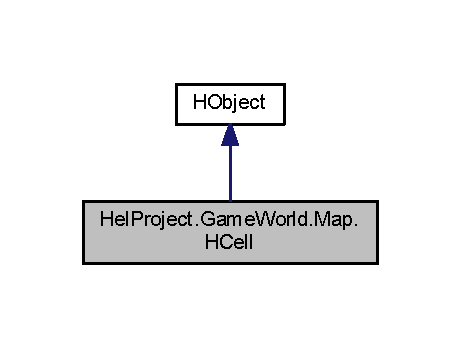
\includegraphics[width=221pt]{class_hel_project_1_1_game_world_1_1_map_1_1_h_cell__inherit__graph}
\end{center}
\end{figure}


Collaboration diagram for Hel\+Project.\+Game\+World.\+Map.\+H\+Cell\+:\nopagebreak
\begin{figure}[H]
\begin{center}
\leavevmode
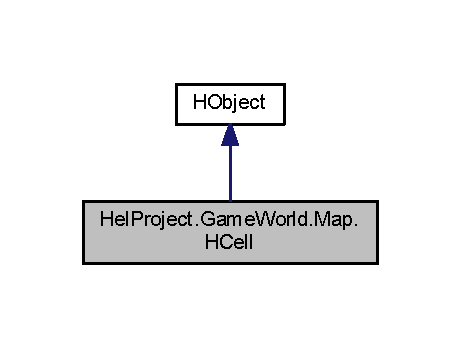
\includegraphics[width=221pt]{class_hel_project_1_1_game_world_1_1_map_1_1_h_cell__coll__graph}
\end{center}
\end{figure}
\subsection*{Public Member Functions}
\begin{DoxyCompactItemize}
\item 
\hyperlink{class_hel_project_1_1_game_world_1_1_map_1_1_h_cell_a668a877ddffe6ff8e1dca674214a9c3d}{H\+Cell} ()
\begin{DoxyCompactList}\small\item\em Cell that represents a part of the map \end{DoxyCompactList}\item 
\hyperlink{class_hel_project_1_1_game_world_1_1_map_1_1_h_cell_a32bbca9e2eadd8aeeb956629418f00f1}{H\+Cell} (Vector2 position)
\begin{DoxyCompactList}\small\item\em Cell that represents a part of the map \end{DoxyCompactList}\item 
\hyperlink{class_hel_project_1_1_game_world_1_1_map_1_1_h_cell_ac17c0998ae60d46ea3b6e1d7ca29e54e}{H\+Cell} (bool is\+Walkable, Vector2 position)
\begin{DoxyCompactList}\small\item\em Cell that represents a part of the map \end{DoxyCompactList}\item 
\hyperlink{class_hel_project_1_1_game_world_1_1_map_1_1_h_cell_a3660e3a5fc19aae5e1188f73330d645b}{H\+Cell} (bool is\+Walkable, Vector2 position, string type)
\begin{DoxyCompactList}\small\item\em Cell that represents a part of the map \end{DoxyCompactList}\end{DoxyCompactItemize}
\subsection*{Public Attributes}
\begin{DoxyCompactItemize}
\item 
\hypertarget{class_hel_project_1_1_game_world_1_1_map_1_1_h_cell_ae39c780d2536601254122162487f8a79}{}const int {\bfseries T\+I\+L\+E\+\_\+\+S\+I\+Z\+E} = 32\label{class_hel_project_1_1_game_world_1_1_map_1_1_h_cell_ae39c780d2536601254122162487f8a79}

\end{DoxyCompactItemize}
\subsection*{Properties}
\begin{DoxyCompactItemize}
\item 
\hyperlink{class_hel_project_1_1_tools_1_1_f_rectangle}{F\+Rectangle} \hyperlink{class_hel_project_1_1_game_world_1_1_map_1_1_h_cell_a04c8b19e74486d6a2c05b700895290aa}{Bounds}\hspace{0.3cm}{\ttfamily  \mbox{[}get, set\mbox{]}}
\begin{DoxyCompactList}\small\item\em Bounds of the cells \end{DoxyCompactList}\item 
string \hyperlink{class_hel_project_1_1_game_world_1_1_map_1_1_h_cell_a5565694259c3692972bea83e774a1012}{Type}\hspace{0.3cm}{\ttfamily  \mbox{[}get, set\mbox{]}}
\begin{DoxyCompactList}\small\item\em Type of the cell \end{DoxyCompactList}\end{DoxyCompactItemize}
\subsection*{Additional Inherited Members}


\subsection{Detailed Description}
Cell of a map 



\subsection{Constructor \& Destructor Documentation}
\hypertarget{class_hel_project_1_1_game_world_1_1_map_1_1_h_cell_a668a877ddffe6ff8e1dca674214a9c3d}{}\index{Hel\+Project\+::\+Game\+World\+::\+Map\+::\+H\+Cell@{Hel\+Project\+::\+Game\+World\+::\+Map\+::\+H\+Cell}!H\+Cell@{H\+Cell}}
\index{H\+Cell@{H\+Cell}!Hel\+Project\+::\+Game\+World\+::\+Map\+::\+H\+Cell@{Hel\+Project\+::\+Game\+World\+::\+Map\+::\+H\+Cell}}
\subsubsection[{H\+Cell}]{\setlength{\rightskip}{0pt plus 5cm}Hel\+Project.\+Game\+World.\+Map.\+H\+Cell.\+H\+Cell (
\begin{DoxyParamCaption}
{}
\end{DoxyParamCaption}
)}\label{class_hel_project_1_1_game_world_1_1_map_1_1_h_cell_a668a877ddffe6ff8e1dca674214a9c3d}


Cell that represents a part of the map 

\hypertarget{class_hel_project_1_1_game_world_1_1_map_1_1_h_cell_a32bbca9e2eadd8aeeb956629418f00f1}{}\index{Hel\+Project\+::\+Game\+World\+::\+Map\+::\+H\+Cell@{Hel\+Project\+::\+Game\+World\+::\+Map\+::\+H\+Cell}!H\+Cell@{H\+Cell}}
\index{H\+Cell@{H\+Cell}!Hel\+Project\+::\+Game\+World\+::\+Map\+::\+H\+Cell@{Hel\+Project\+::\+Game\+World\+::\+Map\+::\+H\+Cell}}
\subsubsection[{H\+Cell}]{\setlength{\rightskip}{0pt plus 5cm}Hel\+Project.\+Game\+World.\+Map.\+H\+Cell.\+H\+Cell (
\begin{DoxyParamCaption}
\item[{Vector2}]{position}
\end{DoxyParamCaption}
)}\label{class_hel_project_1_1_game_world_1_1_map_1_1_h_cell_a32bbca9e2eadd8aeeb956629418f00f1}


Cell that represents a part of the map 


\begin{DoxyParams}{Parameters}
{\em position} & The position of the cell\\
\hline
\end{DoxyParams}


The cell position is rounded to the base digit. \hypertarget{class_hel_project_1_1_game_world_1_1_map_1_1_h_cell_ac17c0998ae60d46ea3b6e1d7ca29e54e}{}\index{Hel\+Project\+::\+Game\+World\+::\+Map\+::\+H\+Cell@{Hel\+Project\+::\+Game\+World\+::\+Map\+::\+H\+Cell}!H\+Cell@{H\+Cell}}
\index{H\+Cell@{H\+Cell}!Hel\+Project\+::\+Game\+World\+::\+Map\+::\+H\+Cell@{Hel\+Project\+::\+Game\+World\+::\+Map\+::\+H\+Cell}}
\subsubsection[{H\+Cell}]{\setlength{\rightskip}{0pt plus 5cm}Hel\+Project.\+Game\+World.\+Map.\+H\+Cell.\+H\+Cell (
\begin{DoxyParamCaption}
\item[{bool}]{is\+Walkable, }
\item[{Vector2}]{position}
\end{DoxyParamCaption}
)}\label{class_hel_project_1_1_game_world_1_1_map_1_1_h_cell_ac17c0998ae60d46ea3b6e1d7ca29e54e}


Cell that represents a part of the map 


\begin{DoxyParams}{Parameters}
{\em is\+Walkable} & The cell can be \textquotesingle{}walked\textquotesingle{} on by entities\\
\hline
{\em position} & The position of the cell\\
\hline
\end{DoxyParams}


The cell position is rounded to the base digit. \hypertarget{class_hel_project_1_1_game_world_1_1_map_1_1_h_cell_a3660e3a5fc19aae5e1188f73330d645b}{}\index{Hel\+Project\+::\+Game\+World\+::\+Map\+::\+H\+Cell@{Hel\+Project\+::\+Game\+World\+::\+Map\+::\+H\+Cell}!H\+Cell@{H\+Cell}}
\index{H\+Cell@{H\+Cell}!Hel\+Project\+::\+Game\+World\+::\+Map\+::\+H\+Cell@{Hel\+Project\+::\+Game\+World\+::\+Map\+::\+H\+Cell}}
\subsubsection[{H\+Cell}]{\setlength{\rightskip}{0pt plus 5cm}Hel\+Project.\+Game\+World.\+Map.\+H\+Cell.\+H\+Cell (
\begin{DoxyParamCaption}
\item[{bool}]{is\+Walkable, }
\item[{Vector2}]{position, }
\item[{string}]{type}
\end{DoxyParamCaption}
)}\label{class_hel_project_1_1_game_world_1_1_map_1_1_h_cell_a3660e3a5fc19aae5e1188f73330d645b}


Cell that represents a part of the map 


\begin{DoxyParams}{Parameters}
{\em is\+Walkable} & The cell can be \textquotesingle{}walked\textquotesingle{} on by entities\\
\hline
{\em position} & The position of the cell\\
\hline
{\em type} & Type of the cell\\
\hline
\end{DoxyParams}


The cell position is rounded to the base digit. The type of the often corresponds with a texture 

\subsection{Property Documentation}
\hypertarget{class_hel_project_1_1_game_world_1_1_map_1_1_h_cell_a04c8b19e74486d6a2c05b700895290aa}{}\index{Hel\+Project\+::\+Game\+World\+::\+Map\+::\+H\+Cell@{Hel\+Project\+::\+Game\+World\+::\+Map\+::\+H\+Cell}!Bounds@{Bounds}}
\index{Bounds@{Bounds}!Hel\+Project\+::\+Game\+World\+::\+Map\+::\+H\+Cell@{Hel\+Project\+::\+Game\+World\+::\+Map\+::\+H\+Cell}}
\subsubsection[{Bounds}]{\setlength{\rightskip}{0pt plus 5cm}{\bf F\+Rectangle} Hel\+Project.\+Game\+World.\+Map.\+H\+Cell.\+Bounds\hspace{0.3cm}{\ttfamily [get]}, {\ttfamily [set]}}\label{class_hel_project_1_1_game_world_1_1_map_1_1_h_cell_a04c8b19e74486d6a2c05b700895290aa}


Bounds of the cells 

\hypertarget{class_hel_project_1_1_game_world_1_1_map_1_1_h_cell_a5565694259c3692972bea83e774a1012}{}\index{Hel\+Project\+::\+Game\+World\+::\+Map\+::\+H\+Cell@{Hel\+Project\+::\+Game\+World\+::\+Map\+::\+H\+Cell}!Type@{Type}}
\index{Type@{Type}!Hel\+Project\+::\+Game\+World\+::\+Map\+::\+H\+Cell@{Hel\+Project\+::\+Game\+World\+::\+Map\+::\+H\+Cell}}
\subsubsection[{Type}]{\setlength{\rightskip}{0pt plus 5cm}string Hel\+Project.\+Game\+World.\+Map.\+H\+Cell.\+Type\hspace{0.3cm}{\ttfamily [get]}, {\ttfamily [set]}}\label{class_hel_project_1_1_game_world_1_1_map_1_1_h_cell_a5565694259c3692972bea83e774a1012}


Type of the cell 

Often corresponds with a texture 

The documentation for this class was generated from the following file\+:\begin{DoxyCompactItemize}
\item 
src/\+Hel\+Project/\+Game\+World/\+Map/H\+Cell.\+cs\end{DoxyCompactItemize}

\hypertarget{class_hel_project_1_1_game_world_1_1_entities_1_1_h_entity}{}\section{Hel\+Project.\+Game\+World.\+Entities.\+H\+Entity Class Reference}
\label{class_hel_project_1_1_game_world_1_1_entities_1_1_h_entity}\index{Hel\+Project.\+Game\+World.\+Entities.\+H\+Entity@{Hel\+Project.\+Game\+World.\+Entities.\+H\+Entity}}


Inheritance diagram for Hel\+Project.\+Game\+World.\+Entities.\+H\+Entity\+:
% FIG 0


Collaboration diagram for Hel\+Project.\+Game\+World.\+Entities.\+H\+Entity\+:
% FIG 1
\subsection*{Public Member Functions}
\begin{DoxyCompactItemize}
\item 
\hyperlink{class_hel_project_1_1_game_world_1_1_entities_1_1_h_entity_a0f76dfa203f3b1802a15d809b4c33170}{H\+Entity} ()
\begin{DoxyCompactList}\small\item\em Creates an entity \end{DoxyCompactList}\item 
\hyperlink{class_hel_project_1_1_game_world_1_1_entities_1_1_h_entity_a7d78007869c12e256a2837c9d4733b40}{H\+Entity} (\hyperlink{class_hel_project_1_1_tools_1_1_f_position}{F\+Position} position)
\begin{DoxyCompactList}\small\item\em Creates an entity \end{DoxyCompactList}\item 
\hyperlink{class_hel_project_1_1_game_world_1_1_entities_1_1_h_entity_affca20b99d4d8791ffe00fb96ad7a9e0}{H\+Entity} (\hyperlink{class_hel_project_1_1_features_1_1_feature_collection}{Feature\+Collection} initial\+Features, \hyperlink{class_hel_project_1_1_tools_1_1_f_position}{F\+Position} position)
\begin{DoxyCompactList}\small\item\em Creates an entity \end{DoxyCompactList}\end{DoxyCompactItemize}
\subsection*{Public Attributes}
\begin{DoxyCompactItemize}
\item 
\hypertarget{class_hel_project_1_1_game_world_1_1_entities_1_1_h_entity_aad8b19d7624ef5273487147d2bed4861}{}const float {\bfseries D\+E\+F\+A\+U\+L\+T\+\_\+\+S\+T\+R\+E\+N\+G\+H\+T} = 5.\+0f\label{class_hel_project_1_1_game_world_1_1_entities_1_1_h_entity_aad8b19d7624ef5273487147d2bed4861}

\item 
\hypertarget{class_hel_project_1_1_game_world_1_1_entities_1_1_h_entity_af2a9d375e692a163f12f6721b9ac8ed6}{}const float {\bfseries D\+E\+F\+A\+U\+L\+T\+\_\+\+A\+G\+I\+L\+I\+T\+Y} = 5.\+0f\label{class_hel_project_1_1_game_world_1_1_entities_1_1_h_entity_af2a9d375e692a163f12f6721b9ac8ed6}

\item 
\hypertarget{class_hel_project_1_1_game_world_1_1_entities_1_1_h_entity_aafd34a030458f78c8b4246483e2dcdd7}{}const float {\bfseries D\+E\+F\+A\+U\+L\+T\+\_\+\+V\+I\+T\+A\+L\+I\+T\+Y} = 5.\+0f\label{class_hel_project_1_1_game_world_1_1_entities_1_1_h_entity_aafd34a030458f78c8b4246483e2dcdd7}

\item 
\hypertarget{class_hel_project_1_1_game_world_1_1_entities_1_1_h_entity_a4d89bdd6367c78dc8742f291ca4d9ab0}{}const float {\bfseries D\+E\+F\+A\+U\+L\+T\+\_\+\+M\+A\+G\+I\+C} = 5.\+0f\label{class_hel_project_1_1_game_world_1_1_entities_1_1_h_entity_a4d89bdd6367c78dc8742f291ca4d9ab0}

\item 
\hypertarget{class_hel_project_1_1_game_world_1_1_entities_1_1_h_entity_aeea5a00e7035b51582029bacb080e92f}{}const float {\bfseries D\+E\+F\+A\+U\+L\+T\+\_\+\+A\+T\+T\+A\+C\+K\+S\+P\+E\+E\+D} = 0.\+6f\label{class_hel_project_1_1_game_world_1_1_entities_1_1_h_entity_aeea5a00e7035b51582029bacb080e92f}

\item 
\hypertarget{class_hel_project_1_1_game_world_1_1_entities_1_1_h_entity_aa016bdcd02e53ba55381c99c83a456e6}{}const float {\bfseries D\+E\+F\+A\+U\+L\+T\+\_\+\+M\+I\+N\+U\+M\+U\+M\+D\+A\+M\+A\+G\+E} = 1.\+0f\label{class_hel_project_1_1_game_world_1_1_entities_1_1_h_entity_aa016bdcd02e53ba55381c99c83a456e6}

\item 
\hypertarget{class_hel_project_1_1_game_world_1_1_entities_1_1_h_entity_a1c7a66aa3a3ddf816ad32502c5e64f20}{}const float {\bfseries D\+E\+F\+A\+U\+L\+T\+\_\+\+M\+A\+X\+I\+M\+U\+M\+D\+A\+M\+A\+G\+E} = 3.\+0f\label{class_hel_project_1_1_game_world_1_1_entities_1_1_h_entity_a1c7a66aa3a3ddf816ad32502c5e64f20}

\item 
\hypertarget{class_hel_project_1_1_game_world_1_1_entities_1_1_h_entity_a229cc4748e88bdd90d6d0e022d677a81}{}const float {\bfseries D\+E\+F\+A\+U\+L\+T\+\_\+\+M\+A\+N\+A\+R\+E\+G\+E\+N\+E\+R\+A\+T\+I\+O\+N} = 1.\+0f\label{class_hel_project_1_1_game_world_1_1_entities_1_1_h_entity_a229cc4748e88bdd90d6d0e022d677a81}

\item 
\hypertarget{class_hel_project_1_1_game_world_1_1_entities_1_1_h_entity_a241e7ce5f78fb186cc2379e2b714fe9f}{}const float {\bfseries D\+E\+F\+A\+U\+L\+T\+\_\+\+M\+O\+V\+E\+M\+E\+N\+T\+S\+P\+E\+E\+D} = 1.\+0f\label{class_hel_project_1_1_game_world_1_1_entities_1_1_h_entity_a241e7ce5f78fb186cc2379e2b714fe9f}

\item 
\hypertarget{class_hel_project_1_1_game_world_1_1_entities_1_1_h_entity_a3ae3951348143dcec12a91af4d95f7d5}{}const float {\bfseries D\+E\+F\+A\+U\+L\+T\+\_\+\+L\+I\+F\+E\+P\+O\+I\+N\+T\+S} = 100.\+0f\label{class_hel_project_1_1_game_world_1_1_entities_1_1_h_entity_a3ae3951348143dcec12a91af4d95f7d5}

\end{DoxyCompactItemize}
\subsection*{Properties}
\begin{DoxyCompactItemize}
\item 
\hyperlink{class_hel_project_1_1_features_1_1_feature_collection}{Feature\+Collection} \hyperlink{class_hel_project_1_1_game_world_1_1_entities_1_1_h_entity_afb7fd74a8073bf8311bceba415e6022c}{Maximized\+Features}\hspace{0.3cm}{\ttfamily  \mbox{[}get, set\mbox{]}}
\begin{DoxyCompactList}\small\item\em Maximized features \end{DoxyCompactList}\item 
\hyperlink{class_hel_project_1_1_features_1_1_feature_manager}{Feature\+Manager} \hyperlink{class_hel_project_1_1_game_world_1_1_entities_1_1_h_entity_a80aaee359bc963011a0f34c1f27aa47c}{Feature\+Calculator}\hspace{0.3cm}{\ttfamily  \mbox{[}get, set\mbox{]}}
\begin{DoxyCompactList}\small\item\em Feature manager to calculate the actual features \end{DoxyCompactList}\item 
\hyperlink{class_hel_project_1_1_features_1_1_feature_collection}{Feature\+Collection} \hyperlink{class_hel_project_1_1_game_world_1_1_entities_1_1_h_entity_ad2f5977677a00f45a3402f11391e8282}{Actual\+Features}\hspace{0.3cm}{\ttfamily  \mbox{[}get, set\mbox{]}}
\begin{DoxyCompactList}\small\item\em Actual features of the entity \end{DoxyCompactList}\item 
\hyperlink{class_hel_project_1_1_features_1_1_feature_collection}{Feature\+Collection} \hyperlink{class_hel_project_1_1_game_world_1_1_entities_1_1_h_entity_a155d3d12d931e900e26d770c120ec361}{Initial\+Features}\hspace{0.3cm}{\ttfamily  \mbox{[}get, set\mbox{]}}
\begin{DoxyCompactList}\small\item\em Initial feature of the entity \end{DoxyCompactList}\end{DoxyCompactItemize}
\subsection*{Additional Inherited Members}


\subsection{Constructor \& Destructor Documentation}
\hypertarget{class_hel_project_1_1_game_world_1_1_entities_1_1_h_entity_a0f76dfa203f3b1802a15d809b4c33170}{}\index{Hel\+Project\+::\+Game\+World\+::\+Entities\+::\+H\+Entity@{Hel\+Project\+::\+Game\+World\+::\+Entities\+::\+H\+Entity}!H\+Entity@{H\+Entity}}
\index{H\+Entity@{H\+Entity}!Hel\+Project\+::\+Game\+World\+::\+Entities\+::\+H\+Entity@{Hel\+Project\+::\+Game\+World\+::\+Entities\+::\+H\+Entity}}
\subsubsection[{H\+Entity}]{\setlength{\rightskip}{0pt plus 5cm}Hel\+Project.\+Game\+World.\+Entities.\+H\+Entity.\+H\+Entity (
\begin{DoxyParamCaption}
{}
\end{DoxyParamCaption}
)}\label{class_hel_project_1_1_game_world_1_1_entities_1_1_h_entity_a0f76dfa203f3b1802a15d809b4c33170}


Creates an entity 

\hypertarget{class_hel_project_1_1_game_world_1_1_entities_1_1_h_entity_a7d78007869c12e256a2837c9d4733b40}{}\index{Hel\+Project\+::\+Game\+World\+::\+Entities\+::\+H\+Entity@{Hel\+Project\+::\+Game\+World\+::\+Entities\+::\+H\+Entity}!H\+Entity@{H\+Entity}}
\index{H\+Entity@{H\+Entity}!Hel\+Project\+::\+Game\+World\+::\+Entities\+::\+H\+Entity@{Hel\+Project\+::\+Game\+World\+::\+Entities\+::\+H\+Entity}}
\subsubsection[{H\+Entity}]{\setlength{\rightskip}{0pt plus 5cm}Hel\+Project.\+Game\+World.\+Entities.\+H\+Entity.\+H\+Entity (
\begin{DoxyParamCaption}
\item[{{\bf F\+Position}}]{position}
\end{DoxyParamCaption}
)}\label{class_hel_project_1_1_game_world_1_1_entities_1_1_h_entity_a7d78007869c12e256a2837c9d4733b40}


Creates an entity 


\begin{DoxyParams}{Parameters}
{\em position} & Position of the entity\\
\hline
\end{DoxyParams}
\hypertarget{class_hel_project_1_1_game_world_1_1_entities_1_1_h_entity_affca20b99d4d8791ffe00fb96ad7a9e0}{}\index{Hel\+Project\+::\+Game\+World\+::\+Entities\+::\+H\+Entity@{Hel\+Project\+::\+Game\+World\+::\+Entities\+::\+H\+Entity}!H\+Entity@{H\+Entity}}
\index{H\+Entity@{H\+Entity}!Hel\+Project\+::\+Game\+World\+::\+Entities\+::\+H\+Entity@{Hel\+Project\+::\+Game\+World\+::\+Entities\+::\+H\+Entity}}
\subsubsection[{H\+Entity}]{\setlength{\rightskip}{0pt plus 5cm}Hel\+Project.\+Game\+World.\+Entities.\+H\+Entity.\+H\+Entity (
\begin{DoxyParamCaption}
\item[{{\bf Feature\+Collection}}]{initial\+Features, }
\item[{{\bf F\+Position}}]{position}
\end{DoxyParamCaption}
)}\label{class_hel_project_1_1_game_world_1_1_entities_1_1_h_entity_affca20b99d4d8791ffe00fb96ad7a9e0}


Creates an entity 


\begin{DoxyParams}{Parameters}
{\em initial\+Features} & Initial \hyperlink{namespace_hel_project_1_1_features}{Features} of the enitity\\
\hline
{\em position} & Position of the entity\\
\hline
{\em life\+Points} & Life points of the entity\\
\hline
\end{DoxyParams}


\subsection{Property Documentation}
\hypertarget{class_hel_project_1_1_game_world_1_1_entities_1_1_h_entity_ad2f5977677a00f45a3402f11391e8282}{}\index{Hel\+Project\+::\+Game\+World\+::\+Entities\+::\+H\+Entity@{Hel\+Project\+::\+Game\+World\+::\+Entities\+::\+H\+Entity}!Actual\+Features@{Actual\+Features}}
\index{Actual\+Features@{Actual\+Features}!Hel\+Project\+::\+Game\+World\+::\+Entities\+::\+H\+Entity@{Hel\+Project\+::\+Game\+World\+::\+Entities\+::\+H\+Entity}}
\subsubsection[{Actual\+Features}]{\setlength{\rightskip}{0pt plus 5cm}{\bf Feature\+Collection} Hel\+Project.\+Game\+World.\+Entities.\+H\+Entity.\+Actual\+Features\hspace{0.3cm}{\ttfamily [get]}, {\ttfamily [set]}}\label{class_hel_project_1_1_game_world_1_1_entities_1_1_h_entity_ad2f5977677a00f45a3402f11391e8282}


Actual features of the entity 

\hypertarget{class_hel_project_1_1_game_world_1_1_entities_1_1_h_entity_a80aaee359bc963011a0f34c1f27aa47c}{}\index{Hel\+Project\+::\+Game\+World\+::\+Entities\+::\+H\+Entity@{Hel\+Project\+::\+Game\+World\+::\+Entities\+::\+H\+Entity}!Feature\+Calculator@{Feature\+Calculator}}
\index{Feature\+Calculator@{Feature\+Calculator}!Hel\+Project\+::\+Game\+World\+::\+Entities\+::\+H\+Entity@{Hel\+Project\+::\+Game\+World\+::\+Entities\+::\+H\+Entity}}
\subsubsection[{Feature\+Calculator}]{\setlength{\rightskip}{0pt plus 5cm}{\bf Feature\+Manager} Hel\+Project.\+Game\+World.\+Entities.\+H\+Entity.\+Feature\+Calculator\hspace{0.3cm}{\ttfamily [get]}, {\ttfamily [set]}}\label{class_hel_project_1_1_game_world_1_1_entities_1_1_h_entity_a80aaee359bc963011a0f34c1f27aa47c}


Feature manager to calculate the actual features 

\hypertarget{class_hel_project_1_1_game_world_1_1_entities_1_1_h_entity_a155d3d12d931e900e26d770c120ec361}{}\index{Hel\+Project\+::\+Game\+World\+::\+Entities\+::\+H\+Entity@{Hel\+Project\+::\+Game\+World\+::\+Entities\+::\+H\+Entity}!Initial\+Features@{Initial\+Features}}
\index{Initial\+Features@{Initial\+Features}!Hel\+Project\+::\+Game\+World\+::\+Entities\+::\+H\+Entity@{Hel\+Project\+::\+Game\+World\+::\+Entities\+::\+H\+Entity}}
\subsubsection[{Initial\+Features}]{\setlength{\rightskip}{0pt plus 5cm}{\bf Feature\+Collection} Hel\+Project.\+Game\+World.\+Entities.\+H\+Entity.\+Initial\+Features\hspace{0.3cm}{\ttfamily [get]}, {\ttfamily [set]}}\label{class_hel_project_1_1_game_world_1_1_entities_1_1_h_entity_a155d3d12d931e900e26d770c120ec361}


Initial feature of the entity 

\hypertarget{class_hel_project_1_1_game_world_1_1_entities_1_1_h_entity_afb7fd74a8073bf8311bceba415e6022c}{}\index{Hel\+Project\+::\+Game\+World\+::\+Entities\+::\+H\+Entity@{Hel\+Project\+::\+Game\+World\+::\+Entities\+::\+H\+Entity}!Maximized\+Features@{Maximized\+Features}}
\index{Maximized\+Features@{Maximized\+Features}!Hel\+Project\+::\+Game\+World\+::\+Entities\+::\+H\+Entity@{Hel\+Project\+::\+Game\+World\+::\+Entities\+::\+H\+Entity}}
\subsubsection[{Maximized\+Features}]{\setlength{\rightskip}{0pt plus 5cm}{\bf Feature\+Collection} Hel\+Project.\+Game\+World.\+Entities.\+H\+Entity.\+Maximized\+Features\hspace{0.3cm}{\ttfamily [get]}, {\ttfamily [set]}}\label{class_hel_project_1_1_game_world_1_1_entities_1_1_h_entity_afb7fd74a8073bf8311bceba415e6022c}


Maximized features 



The documentation for this class was generated from the following file\+:\begin{DoxyCompactItemize}
\item 
src/\+Hel\+Project/\+Game\+World/\+Entities/H\+Entity.\+cs\end{DoxyCompactItemize}

\hypertarget{class_hel_project_1_1_game_world_1_1_entities_1_1_h_hero}{}\section{Hel\+Project.\+Game\+World.\+Entities.\+H\+Hero Class Reference}
\label{class_hel_project_1_1_game_world_1_1_entities_1_1_h_hero}\index{Hel\+Project.\+Game\+World.\+Entities.\+H\+Hero@{Hel\+Project.\+Game\+World.\+Entities.\+H\+Hero}}


The documentation for this class was generated from the following file\+:\begin{DoxyCompactItemize}
\item 
src/\+Hel\+Project/\+Game\+World/\+Entities/H\+Hero.\+cs\end{DoxyCompactItemize}

\hypertarget{class_hel_project_1_1_game_world_1_1_entities_1_1_h_hostile}{}\section{Hel\+Project.\+Game\+World.\+Entities.\+H\+Hostile Class Reference}
\label{class_hel_project_1_1_game_world_1_1_entities_1_1_h_hostile}\index{Hel\+Project.\+Game\+World.\+Entities.\+H\+Hostile@{Hel\+Project.\+Game\+World.\+Entities.\+H\+Hostile}}


Inheritance diagram for Hel\+Project.\+Game\+World.\+Entities.\+H\+Hostile\+:
\nopagebreak
\begin{figure}[H]
\begin{center}
\leavevmode
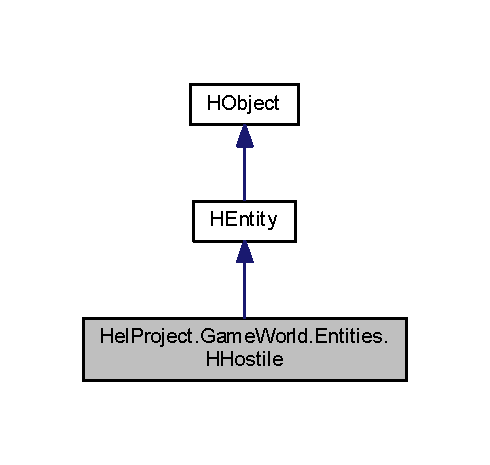
\includegraphics[width=235pt]{class_hel_project_1_1_game_world_1_1_entities_1_1_h_hostile__inherit__graph}
\end{center}
\end{figure}


Collaboration diagram for Hel\+Project.\+Game\+World.\+Entities.\+H\+Hostile\+:
\nopagebreak
\begin{figure}[H]
\begin{center}
\leavevmode
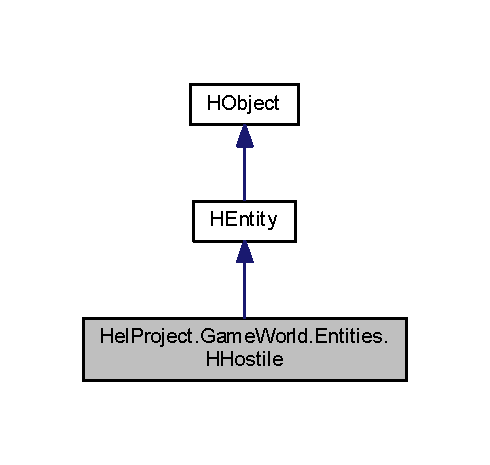
\includegraphics[width=235pt]{class_hel_project_1_1_game_world_1_1_entities_1_1_h_hostile__coll__graph}
\end{center}
\end{figure}
\subsection*{Public Member Functions}
\begin{DoxyCompactItemize}
\item 
\hyperlink{class_hel_project_1_1_game_world_1_1_entities_1_1_h_hostile_a7b71c02b0f22735687ef5c68529837de}{H\+Hostile} (\hyperlink{class_hel_project_1_1_features_1_1_feature_collection}{Feature\+Collection} initial\+Features, Vector2 position, float width, float height, string texture\+Name, float field\+Of\+View=8.\+125f)
\begin{DoxyCompactList}\small\item\em Creates a hostile creature \end{DoxyCompactList}\item 
override void \hyperlink{class_hel_project_1_1_game_world_1_1_entities_1_1_h_hostile_ab244ce132ea02c1e4bf9e38f199dbe85}{Load\+Content} ()
\begin{DoxyCompactList}\small\item\em Loads the content of the hostile \end{DoxyCompactList}\item 
override void \hyperlink{class_hel_project_1_1_game_world_1_1_entities_1_1_h_hostile_a43c15c63adde7e4bb5747625a40789d7}{Unload\+Content} ()
\begin{DoxyCompactList}\small\item\em Unloads the content of the hostile \end{DoxyCompactList}\item 
override void \hyperlink{class_hel_project_1_1_game_world_1_1_entities_1_1_h_hostile_a3ce954aa41e47c306487d94ba64ae822}{Update} (Game\+Time game\+Time)
\begin{DoxyCompactList}\small\item\em Updates the mechanismes of the hostile \end{DoxyCompactList}\item 
override void \hyperlink{class_hel_project_1_1_game_world_1_1_entities_1_1_h_hostile_a548b6f33addf42cbe85d4058ace51d76}{Draw} (Sprite\+Batch sprite\+Batch)
\begin{DoxyCompactList}\small\item\em Draws the hostile \end{DoxyCompactList}\end{DoxyCompactItemize}
\subsection*{Properties}
\begin{DoxyCompactItemize}
\item 
\hyperlink{class_hel_project_1_1_u_i_1_1_h_u_d_1_1_filling_bar}{Filling\+Bar} \hyperlink{class_hel_project_1_1_game_world_1_1_entities_1_1_h_hostile_af213001320773aa02dccb5132b4314f8}{Health\+Bar}\hspace{0.3cm}{\ttfamily  \mbox{[}get, set\mbox{]}}
\begin{DoxyCompactList}\small\item\em Health bar of the hostile \end{DoxyCompactList}\item 
bool \hyperlink{class_hel_project_1_1_game_world_1_1_entities_1_1_h_hostile_a6342a67533fe79ee3fac54c5006248a9}{Is\+Alerted}\hspace{0.3cm}{\ttfamily  \mbox{[}get, set\mbox{]}}
\begin{DoxyCompactList}\small\item\em The unit is alerted \end{DoxyCompactList}\item 
\hyperlink{class_hel_project_1_1_tools_1_1_f_rectangle}{F\+Rectangle} \hyperlink{class_hel_project_1_1_game_world_1_1_entities_1_1_h_hostile_ae9b043f35166b59e96a84778894b12db}{Field\+Of\+View}\hspace{0.3cm}{\ttfamily  \mbox{[}get, set\mbox{]}}
\begin{DoxyCompactList}\small\item\em Field of view of the hostile \end{DoxyCompactList}\item 
\hyperlink{class_hel_project_1_1_tools_1_1_f_rectangle}{F\+Rectangle} \hyperlink{class_hel_project_1_1_game_world_1_1_entities_1_1_h_hostile_afbd9573b6ebd47b3accade7d26f99675}{Alerted\+Field\+Of\+View}\hspace{0.3cm}{\ttfamily  \mbox{[}get, set\mbox{]}}
\begin{DoxyCompactList}\small\item\em Field of view of the hositle when this one is alerted \end{DoxyCompactList}\end{DoxyCompactItemize}
\subsection*{Additional Inherited Members}


\subsection{Constructor \& Destructor Documentation}
\hypertarget{class_hel_project_1_1_game_world_1_1_entities_1_1_h_hostile_a7b71c02b0f22735687ef5c68529837de}{}\index{Hel\+Project\+::\+Game\+World\+::\+Entities\+::\+H\+Hostile@{Hel\+Project\+::\+Game\+World\+::\+Entities\+::\+H\+Hostile}!H\+Hostile@{H\+Hostile}}
\index{H\+Hostile@{H\+Hostile}!Hel\+Project\+::\+Game\+World\+::\+Entities\+::\+H\+Hostile@{Hel\+Project\+::\+Game\+World\+::\+Entities\+::\+H\+Hostile}}
\subsubsection[{H\+Hostile}]{\setlength{\rightskip}{0pt plus 5cm}Hel\+Project.\+Game\+World.\+Entities.\+H\+Hostile.\+H\+Hostile (
\begin{DoxyParamCaption}
\item[{{\bf Feature\+Collection}}]{initial\+Features, }
\item[{Vector2}]{position, }
\item[{float}]{width, }
\item[{float}]{height, }
\item[{string}]{texture\+Name, }
\item[{float}]{field\+Of\+View = {\ttfamily 8.125f}}
\end{DoxyParamCaption}
)}\label{class_hel_project_1_1_game_world_1_1_entities_1_1_h_hostile_a7b71c02b0f22735687ef5c68529837de}


Creates a hostile creature 


\begin{DoxyParams}{Parameters}
{\em initial\+Features} & The initial features\\
\hline
{\em position} & Position\\
\hline
{\em width} & Width (in-\/game unit)\\
\hline
{\em height} & Height (in-\/game unit)\\
\hline
{\em texture\+Name} & Name of the texture\\
\hline
\end{DoxyParams}


\subsection{Member Function Documentation}
\hypertarget{class_hel_project_1_1_game_world_1_1_entities_1_1_h_hostile_a548b6f33addf42cbe85d4058ace51d76}{}\index{Hel\+Project\+::\+Game\+World\+::\+Entities\+::\+H\+Hostile@{Hel\+Project\+::\+Game\+World\+::\+Entities\+::\+H\+Hostile}!Draw@{Draw}}
\index{Draw@{Draw}!Hel\+Project\+::\+Game\+World\+::\+Entities\+::\+H\+Hostile@{Hel\+Project\+::\+Game\+World\+::\+Entities\+::\+H\+Hostile}}
\subsubsection[{Draw}]{\setlength{\rightskip}{0pt plus 5cm}override void Hel\+Project.\+Game\+World.\+Entities.\+H\+Hostile.\+Draw (
\begin{DoxyParamCaption}
\item[{Sprite\+Batch}]{sprite\+Batch}
\end{DoxyParamCaption}
)\hspace{0.3cm}{\ttfamily [virtual]}}\label{class_hel_project_1_1_game_world_1_1_entities_1_1_h_hostile_a548b6f33addf42cbe85d4058ace51d76}


Draws the hostile 


\begin{DoxyParams}{Parameters}
{\em sprite\+Batch} & Sprite batch\\
\hline
\end{DoxyParams}


Reimplemented from \hyperlink{class_hel_project_1_1_game_world_1_1_entities_1_1_h_entity_aac4efdcaa42e096838556aba9345f8d5}{Hel\+Project.\+Game\+World.\+Entities.\+H\+Entity}.

\hypertarget{class_hel_project_1_1_game_world_1_1_entities_1_1_h_hostile_ab244ce132ea02c1e4bf9e38f199dbe85}{}\index{Hel\+Project\+::\+Game\+World\+::\+Entities\+::\+H\+Hostile@{Hel\+Project\+::\+Game\+World\+::\+Entities\+::\+H\+Hostile}!Load\+Content@{Load\+Content}}
\index{Load\+Content@{Load\+Content}!Hel\+Project\+::\+Game\+World\+::\+Entities\+::\+H\+Hostile@{Hel\+Project\+::\+Game\+World\+::\+Entities\+::\+H\+Hostile}}
\subsubsection[{Load\+Content}]{\setlength{\rightskip}{0pt plus 5cm}override void Hel\+Project.\+Game\+World.\+Entities.\+H\+Hostile.\+Load\+Content (
\begin{DoxyParamCaption}
{}
\end{DoxyParamCaption}
)\hspace{0.3cm}{\ttfamily [virtual]}}\label{class_hel_project_1_1_game_world_1_1_entities_1_1_h_hostile_ab244ce132ea02c1e4bf9e38f199dbe85}


Loads the content of the hostile 



Reimplemented from \hyperlink{class_hel_project_1_1_game_world_1_1_h_object_a2de39710b20f7af4e1e2463ca93656f8}{Hel\+Project.\+Game\+World.\+H\+Object}.

\hypertarget{class_hel_project_1_1_game_world_1_1_entities_1_1_h_hostile_a43c15c63adde7e4bb5747625a40789d7}{}\index{Hel\+Project\+::\+Game\+World\+::\+Entities\+::\+H\+Hostile@{Hel\+Project\+::\+Game\+World\+::\+Entities\+::\+H\+Hostile}!Unload\+Content@{Unload\+Content}}
\index{Unload\+Content@{Unload\+Content}!Hel\+Project\+::\+Game\+World\+::\+Entities\+::\+H\+Hostile@{Hel\+Project\+::\+Game\+World\+::\+Entities\+::\+H\+Hostile}}
\subsubsection[{Unload\+Content}]{\setlength{\rightskip}{0pt plus 5cm}override void Hel\+Project.\+Game\+World.\+Entities.\+H\+Hostile.\+Unload\+Content (
\begin{DoxyParamCaption}
{}
\end{DoxyParamCaption}
)\hspace{0.3cm}{\ttfamily [virtual]}}\label{class_hel_project_1_1_game_world_1_1_entities_1_1_h_hostile_a43c15c63adde7e4bb5747625a40789d7}


Unloads the content of the hostile 



Reimplemented from \hyperlink{class_hel_project_1_1_game_world_1_1_h_object_a30efa177423e89a85e45b76fe35d6724}{Hel\+Project.\+Game\+World.\+H\+Object}.

\hypertarget{class_hel_project_1_1_game_world_1_1_entities_1_1_h_hostile_a3ce954aa41e47c306487d94ba64ae822}{}\index{Hel\+Project\+::\+Game\+World\+::\+Entities\+::\+H\+Hostile@{Hel\+Project\+::\+Game\+World\+::\+Entities\+::\+H\+Hostile}!Update@{Update}}
\index{Update@{Update}!Hel\+Project\+::\+Game\+World\+::\+Entities\+::\+H\+Hostile@{Hel\+Project\+::\+Game\+World\+::\+Entities\+::\+H\+Hostile}}
\subsubsection[{Update}]{\setlength{\rightskip}{0pt plus 5cm}override void Hel\+Project.\+Game\+World.\+Entities.\+H\+Hostile.\+Update (
\begin{DoxyParamCaption}
\item[{Game\+Time}]{game\+Time}
\end{DoxyParamCaption}
)\hspace{0.3cm}{\ttfamily [virtual]}}\label{class_hel_project_1_1_game_world_1_1_entities_1_1_h_hostile_a3ce954aa41e47c306487d94ba64ae822}


Updates the mechanismes of the hostile 


\begin{DoxyParams}{Parameters}
{\em game\+Time} & Game time\\
\hline
\end{DoxyParams}


Reimplemented from \hyperlink{class_hel_project_1_1_game_world_1_1_entities_1_1_h_entity_a3feda059e3ebd1a20579260a6dc60291}{Hel\+Project.\+Game\+World.\+Entities.\+H\+Entity}.



\subsection{Property Documentation}
\hypertarget{class_hel_project_1_1_game_world_1_1_entities_1_1_h_hostile_afbd9573b6ebd47b3accade7d26f99675}{}\index{Hel\+Project\+::\+Game\+World\+::\+Entities\+::\+H\+Hostile@{Hel\+Project\+::\+Game\+World\+::\+Entities\+::\+H\+Hostile}!Alerted\+Field\+Of\+View@{Alerted\+Field\+Of\+View}}
\index{Alerted\+Field\+Of\+View@{Alerted\+Field\+Of\+View}!Hel\+Project\+::\+Game\+World\+::\+Entities\+::\+H\+Hostile@{Hel\+Project\+::\+Game\+World\+::\+Entities\+::\+H\+Hostile}}
\subsubsection[{Alerted\+Field\+Of\+View}]{\setlength{\rightskip}{0pt plus 5cm}{\bf F\+Rectangle} Hel\+Project.\+Game\+World.\+Entities.\+H\+Hostile.\+Alerted\+Field\+Of\+View\hspace{0.3cm}{\ttfamily [get]}, {\ttfamily [set]}}\label{class_hel_project_1_1_game_world_1_1_entities_1_1_h_hostile_afbd9573b6ebd47b3accade7d26f99675}


Field of view of the hositle when this one is alerted 

\hypertarget{class_hel_project_1_1_game_world_1_1_entities_1_1_h_hostile_ae9b043f35166b59e96a84778894b12db}{}\index{Hel\+Project\+::\+Game\+World\+::\+Entities\+::\+H\+Hostile@{Hel\+Project\+::\+Game\+World\+::\+Entities\+::\+H\+Hostile}!Field\+Of\+View@{Field\+Of\+View}}
\index{Field\+Of\+View@{Field\+Of\+View}!Hel\+Project\+::\+Game\+World\+::\+Entities\+::\+H\+Hostile@{Hel\+Project\+::\+Game\+World\+::\+Entities\+::\+H\+Hostile}}
\subsubsection[{Field\+Of\+View}]{\setlength{\rightskip}{0pt plus 5cm}{\bf F\+Rectangle} Hel\+Project.\+Game\+World.\+Entities.\+H\+Hostile.\+Field\+Of\+View\hspace{0.3cm}{\ttfamily [get]}, {\ttfamily [set]}}\label{class_hel_project_1_1_game_world_1_1_entities_1_1_h_hostile_ae9b043f35166b59e96a84778894b12db}


Field of view of the hostile 

\hypertarget{class_hel_project_1_1_game_world_1_1_entities_1_1_h_hostile_af213001320773aa02dccb5132b4314f8}{}\index{Hel\+Project\+::\+Game\+World\+::\+Entities\+::\+H\+Hostile@{Hel\+Project\+::\+Game\+World\+::\+Entities\+::\+H\+Hostile}!Health\+Bar@{Health\+Bar}}
\index{Health\+Bar@{Health\+Bar}!Hel\+Project\+::\+Game\+World\+::\+Entities\+::\+H\+Hostile@{Hel\+Project\+::\+Game\+World\+::\+Entities\+::\+H\+Hostile}}
\subsubsection[{Health\+Bar}]{\setlength{\rightskip}{0pt plus 5cm}{\bf Filling\+Bar} Hel\+Project.\+Game\+World.\+Entities.\+H\+Hostile.\+Health\+Bar\hspace{0.3cm}{\ttfamily [get]}, {\ttfamily [set]}}\label{class_hel_project_1_1_game_world_1_1_entities_1_1_h_hostile_af213001320773aa02dccb5132b4314f8}


Health bar of the hostile 

\hypertarget{class_hel_project_1_1_game_world_1_1_entities_1_1_h_hostile_a6342a67533fe79ee3fac54c5006248a9}{}\index{Hel\+Project\+::\+Game\+World\+::\+Entities\+::\+H\+Hostile@{Hel\+Project\+::\+Game\+World\+::\+Entities\+::\+H\+Hostile}!Is\+Alerted@{Is\+Alerted}}
\index{Is\+Alerted@{Is\+Alerted}!Hel\+Project\+::\+Game\+World\+::\+Entities\+::\+H\+Hostile@{Hel\+Project\+::\+Game\+World\+::\+Entities\+::\+H\+Hostile}}
\subsubsection[{Is\+Alerted}]{\setlength{\rightskip}{0pt plus 5cm}bool Hel\+Project.\+Game\+World.\+Entities.\+H\+Hostile.\+Is\+Alerted\hspace{0.3cm}{\ttfamily [get]}, {\ttfamily [set]}}\label{class_hel_project_1_1_game_world_1_1_entities_1_1_h_hostile_a6342a67533fe79ee3fac54c5006248a9}


The unit is alerted 



The documentation for this class was generated from the following file\+:\begin{DoxyCompactItemize}
\item 
src/\+Hel\+Project/\+Game\+World/\+Entities/H\+Hostile.\+cs\end{DoxyCompactItemize}

\hypertarget{class_hel_project_1_1_game_world_1_1_h_item}{}\section{Hel\+Project.\+Game\+World.\+H\+Item Class Reference}
\label{class_hel_project_1_1_game_world_1_1_h_item}\index{Hel\+Project.\+Game\+World.\+H\+Item@{Hel\+Project.\+Game\+World.\+H\+Item}}


Item class  


\subsection*{Public Types}
\begin{DoxyCompactItemize}
\item 
enum \hyperlink{class_hel_project_1_1_game_world_1_1_h_item_a7440e7b22ff0e62bcaf89a513716357b}{Item\+Types} \{ \\*
{\bfseries Sword} = 0, 
{\bfseries Two\+Handed\+Sword} = 1, 
{\bfseries Axe} = 2, 
{\bfseries Two\+Handed\+Axe} = 3, 
\\*
{\bfseries Wand} = 4, 
{\bfseries Staff} = 5, 
{\bfseries Bow} = 6, 
{\bfseries Amulet} = 7, 
\\*
{\bfseries Ring} = 8, 
{\bfseries Shield} = 9, 
{\bfseries Quiver} = 10, 
{\bfseries Power\+Source} = 11, 
\\*
{\bfseries Head} = 12, 
{\bfseries Shoulders} = 13, 
{\bfseries Body} = 14, 
{\bfseries Hands} = 15, 
\\*
{\bfseries Legs} = 16, 
{\bfseries Feet} = 17
 \}
\begin{DoxyCompactList}\small\item\em Item types \end{DoxyCompactList}\end{DoxyCompactItemize}
\subsection*{Public Member Functions}
\begin{DoxyCompactItemize}
\item 
\hyperlink{class_hel_project_1_1_game_world_1_1_h_item_a85c06624c5da360525a7b109c28c3f7e}{H\+Item} (string name, \hyperlink{class_hel_project_1_1_game_world_1_1_h_item_a7440e7b22ff0e62bcaf89a513716357b}{Item\+Types} type, \hyperlink{class_hel_project_1_1_features_1_1_feature_collection}{Feature\+Collection} features)
\begin{DoxyCompactList}\small\item\em Creates an item on the floor \end{DoxyCompactList}\item 
\hyperlink{class_hel_project_1_1_game_world_1_1_h_item_a917513f7394553cfc1069ea042004a2a}{H\+Item} (string name, \hyperlink{class_hel_project_1_1_game_world_1_1_h_item_a7440e7b22ff0e62bcaf89a513716357b}{Item\+Types} type, \hyperlink{class_hel_project_1_1_features_1_1_feature_collection}{Feature\+Collection} features, bool is\+On\+Floor)
\begin{DoxyCompactList}\small\item\em Creates an item \end{DoxyCompactList}\end{DoxyCompactItemize}
\subsection*{Properties}
\begin{DoxyCompactItemize}
\item 
string \hyperlink{class_hel_project_1_1_game_world_1_1_h_item_ad6e286a2833c7a01297544008e6e9e67}{Name}\hspace{0.3cm}{\ttfamily  \mbox{[}get, set\mbox{]}}
\begin{DoxyCompactList}\small\item\em Name of the item \end{DoxyCompactList}\item 
\hyperlink{class_hel_project_1_1_game_world_1_1_h_item_a7440e7b22ff0e62bcaf89a513716357b}{Item\+Types} \hyperlink{class_hel_project_1_1_game_world_1_1_h_item_aeeb877e7d0f3aa3adf04c17c67bb385f}{Item\+Type}\hspace{0.3cm}{\ttfamily  \mbox{[}get, set\mbox{]}}
\begin{DoxyCompactList}\small\item\em Type of the item \end{DoxyCompactList}\item 
bool \hyperlink{class_hel_project_1_1_game_world_1_1_h_item_a5fd0a52b0f490f80d0c7abec4b3293c5}{Is\+On\+Floor}\hspace{0.3cm}{\ttfamily  \mbox{[}get, set\mbox{]}}
\begin{DoxyCompactList}\small\item\em Is the item on the floor \end{DoxyCompactList}\item 
\hyperlink{class_hel_project_1_1_features_1_1_feature_collection}{Feature\+Collection} \hyperlink{class_hel_project_1_1_game_world_1_1_h_item_a62269e669b1ff06f017424341ffd7cb9}{Features}\hspace{0.3cm}{\ttfamily  \mbox{[}get, set\mbox{]}}
\begin{DoxyCompactList}\small\item\em Given features of the item \end{DoxyCompactList}\end{DoxyCompactItemize}


\subsection{Detailed Description}
Item class 



\subsection{Member Enumeration Documentation}
\hypertarget{class_hel_project_1_1_game_world_1_1_h_item_a7440e7b22ff0e62bcaf89a513716357b}{}\index{Hel\+Project\+::\+Game\+World\+::\+H\+Item@{Hel\+Project\+::\+Game\+World\+::\+H\+Item}!Item\+Types@{Item\+Types}}
\index{Item\+Types@{Item\+Types}!Hel\+Project\+::\+Game\+World\+::\+H\+Item@{Hel\+Project\+::\+Game\+World\+::\+H\+Item}}
\subsubsection[{Item\+Types}]{\setlength{\rightskip}{0pt plus 5cm}enum {\bf Hel\+Project.\+Game\+World.\+H\+Item.\+Item\+Types}}\label{class_hel_project_1_1_game_world_1_1_h_item_a7440e7b22ff0e62bcaf89a513716357b}


Item types 

Weapons \+: 0 to 6, Accessories \+: 7 to 11, Armors \+: 12 to 17 

\subsection{Constructor \& Destructor Documentation}
\hypertarget{class_hel_project_1_1_game_world_1_1_h_item_a85c06624c5da360525a7b109c28c3f7e}{}\index{Hel\+Project\+::\+Game\+World\+::\+H\+Item@{Hel\+Project\+::\+Game\+World\+::\+H\+Item}!H\+Item@{H\+Item}}
\index{H\+Item@{H\+Item}!Hel\+Project\+::\+Game\+World\+::\+H\+Item@{Hel\+Project\+::\+Game\+World\+::\+H\+Item}}
\subsubsection[{H\+Item}]{\setlength{\rightskip}{0pt plus 5cm}Hel\+Project.\+Game\+World.\+H\+Item.\+H\+Item (
\begin{DoxyParamCaption}
\item[{string}]{name, }
\item[{{\bf Item\+Types}}]{type, }
\item[{{\bf Feature\+Collection}}]{features}
\end{DoxyParamCaption}
)}\label{class_hel_project_1_1_game_world_1_1_h_item_a85c06624c5da360525a7b109c28c3f7e}


Creates an item on the floor 


\begin{DoxyParams}{Parameters}
{\em name} & Name of the item\\
\hline
{\em type} & Type of the item\\
\hline
{\em features} & Given features of the item\\
\hline
\end{DoxyParams}


Is\+On\+Floor == true \hypertarget{class_hel_project_1_1_game_world_1_1_h_item_a917513f7394553cfc1069ea042004a2a}{}\index{Hel\+Project\+::\+Game\+World\+::\+H\+Item@{Hel\+Project\+::\+Game\+World\+::\+H\+Item}!H\+Item@{H\+Item}}
\index{H\+Item@{H\+Item}!Hel\+Project\+::\+Game\+World\+::\+H\+Item@{Hel\+Project\+::\+Game\+World\+::\+H\+Item}}
\subsubsection[{H\+Item}]{\setlength{\rightskip}{0pt plus 5cm}Hel\+Project.\+Game\+World.\+H\+Item.\+H\+Item (
\begin{DoxyParamCaption}
\item[{string}]{name, }
\item[{{\bf Item\+Types}}]{type, }
\item[{{\bf Feature\+Collection}}]{features, }
\item[{bool}]{is\+On\+Floor}
\end{DoxyParamCaption}
)}\label{class_hel_project_1_1_game_world_1_1_h_item_a917513f7394553cfc1069ea042004a2a}


Creates an item 


\begin{DoxyParams}{Parameters}
{\em name} & Name of the item\\
\hline
{\em type} & Type of the item\\
\hline
{\em features} & Given features of the item\\
\hline
{\em is\+On\+Floor} & Is the item on the floor\\
\hline
\end{DoxyParams}


\subsection{Property Documentation}
\hypertarget{class_hel_project_1_1_game_world_1_1_h_item_a62269e669b1ff06f017424341ffd7cb9}{}\index{Hel\+Project\+::\+Game\+World\+::\+H\+Item@{Hel\+Project\+::\+Game\+World\+::\+H\+Item}!Features@{Features}}
\index{Features@{Features}!Hel\+Project\+::\+Game\+World\+::\+H\+Item@{Hel\+Project\+::\+Game\+World\+::\+H\+Item}}
\subsubsection[{Features}]{\setlength{\rightskip}{0pt plus 5cm}{\bf Feature\+Collection} Hel\+Project.\+Game\+World.\+H\+Item.\+Features\hspace{0.3cm}{\ttfamily [get]}, {\ttfamily [set]}}\label{class_hel_project_1_1_game_world_1_1_h_item_a62269e669b1ff06f017424341ffd7cb9}


Given features of the item 

\hypertarget{class_hel_project_1_1_game_world_1_1_h_item_a5fd0a52b0f490f80d0c7abec4b3293c5}{}\index{Hel\+Project\+::\+Game\+World\+::\+H\+Item@{Hel\+Project\+::\+Game\+World\+::\+H\+Item}!Is\+On\+Floor@{Is\+On\+Floor}}
\index{Is\+On\+Floor@{Is\+On\+Floor}!Hel\+Project\+::\+Game\+World\+::\+H\+Item@{Hel\+Project\+::\+Game\+World\+::\+H\+Item}}
\subsubsection[{Is\+On\+Floor}]{\setlength{\rightskip}{0pt plus 5cm}bool Hel\+Project.\+Game\+World.\+H\+Item.\+Is\+On\+Floor\hspace{0.3cm}{\ttfamily [get]}, {\ttfamily [set]}}\label{class_hel_project_1_1_game_world_1_1_h_item_a5fd0a52b0f490f80d0c7abec4b3293c5}


Is the item on the floor 

\hypertarget{class_hel_project_1_1_game_world_1_1_h_item_aeeb877e7d0f3aa3adf04c17c67bb385f}{}\index{Hel\+Project\+::\+Game\+World\+::\+H\+Item@{Hel\+Project\+::\+Game\+World\+::\+H\+Item}!Item\+Type@{Item\+Type}}
\index{Item\+Type@{Item\+Type}!Hel\+Project\+::\+Game\+World\+::\+H\+Item@{Hel\+Project\+::\+Game\+World\+::\+H\+Item}}
\subsubsection[{Item\+Type}]{\setlength{\rightskip}{0pt plus 5cm}{\bf Item\+Types} Hel\+Project.\+Game\+World.\+H\+Item.\+Item\+Type\hspace{0.3cm}{\ttfamily [get]}, {\ttfamily [set]}}\label{class_hel_project_1_1_game_world_1_1_h_item_aeeb877e7d0f3aa3adf04c17c67bb385f}


Type of the item 

\hypertarget{class_hel_project_1_1_game_world_1_1_h_item_ad6e286a2833c7a01297544008e6e9e67}{}\index{Hel\+Project\+::\+Game\+World\+::\+H\+Item@{Hel\+Project\+::\+Game\+World\+::\+H\+Item}!Name@{Name}}
\index{Name@{Name}!Hel\+Project\+::\+Game\+World\+::\+H\+Item@{Hel\+Project\+::\+Game\+World\+::\+H\+Item}}
\subsubsection[{Name}]{\setlength{\rightskip}{0pt plus 5cm}string Hel\+Project.\+Game\+World.\+H\+Item.\+Name\hspace{0.3cm}{\ttfamily [get]}, {\ttfamily [set]}}\label{class_hel_project_1_1_game_world_1_1_h_item_ad6e286a2833c7a01297544008e6e9e67}


Name of the item 



The documentation for this class was generated from the following file\+:\begin{DoxyCompactItemize}
\item 
src/\+Hel\+Project/\+Game\+World/H\+Item.\+cs\end{DoxyCompactItemize}

\hypertarget{class_hel_project_1_1_game_world_1_1_map_1_1_h_map}{}\section{Hel\+Project.\+Game\+World.\+Map.\+H\+Map Class Reference}
\label{class_hel_project_1_1_game_world_1_1_map_1_1_h_map}\index{Hel\+Project.\+Game\+World.\+Map.\+H\+Map@{Hel\+Project.\+Game\+World.\+Map.\+H\+Map}}


Used the create a map for the game  


\subsection*{Public Member Functions}
\begin{DoxyCompactItemize}
\item 
\hyperlink{class_hel_project_1_1_game_world_1_1_map_1_1_h_map_a93cc2548c1f18d85d09ae9c87affd97f}{H\+Map} (int height, int width, float scale=1.\+0f, int non\+Walkable\+Space\+Percentage=\+H\+Map.\+D\+E\+F\+A\+U\+L\+T\+\_\+\+N\+O\+N\+W\+A\+L\+K\+A\+B\+L\+E\+\_\+\+C\+E\+L\+L\+S\+\_\+\+P\+E\+R\+C\+E\+N\+T\+A\+G\+E)
\begin{DoxyCompactList}\small\item\em Creates a map full of non-\/walkable cells \end{DoxyCompactList}\item 
void \hyperlink{class_hel_project_1_1_game_world_1_1_map_1_1_h_map_a50af4bbf5a7d9fd131c70050798230a1}{Make\+Randomly\+Filled\+Map} ()
\begin{DoxyCompactList}\small\item\em Fills the map randomly with borders \end{DoxyCompactList}\item 
void \hyperlink{class_hel_project_1_1_game_world_1_1_map_1_1_h_map_a866544b2e9b7f536371acf03c7b35403}{Clear\+Map} ()
\begin{DoxyCompactList}\small\item\em Clears the map, all the cells are null \end{DoxyCompactList}\item 
void \hyperlink{class_hel_project_1_1_game_world_1_1_map_1_1_h_map_a644aff42a105d8b2b7a9ad0aa4d9ac94}{Make\+Full\+Map} ()
\begin{DoxyCompactList}\small\item\em Creates a map full of non-\/walkable cells \end{DoxyCompactList}\item 
void \hyperlink{class_hel_project_1_1_game_world_1_1_map_1_1_h_map_a338b82cacb27f45c792f090e6bfc12fe}{Make\+Caverns} (int smoothness=D\+E\+F\+A\+U\+L\+T\+\_\+\+S\+M\+O\+O\+T\+H\+N\+E\+S\+S)
\begin{DoxyCompactList}\small\item\em Transforms the cells in the map to correspond to a cavern \end{DoxyCompactList}\item 
bool \hyperlink{class_hel_project_1_1_game_world_1_1_map_1_1_h_map_a31940bf039491720aed68ac056868f2a}{Place\+Cell\+Logic} (int x, int y)
\begin{DoxyCompactList}\small\item\em Places a walkable cell depending on it\textquotesingle{}s neighbors \end{DoxyCompactList}\item 
int \hyperlink{class_hel_project_1_1_game_world_1_1_map_1_1_h_map_ac11321d7ff766f5ff1a57bfc941d721e}{Get\+Number\+Of\+Adjacent\+Unwalkable\+Cells} (int x, int y, int scope\+X, int scope\+Y)
\begin{DoxyCompactList}\small\item\em Gets the number of adjacent non-\/walkable cells around the specified cell \end{DoxyCompactList}\item 
bool \hyperlink{class_hel_project_1_1_game_world_1_1_map_1_1_h_map_a5bca0c19006ab0058c11ebe44c888df5}{Is\+Cell\+Nonwalkable} (int x, int y)
\begin{DoxyCompactList}\small\item\em Verifies if the specified cell is walkable \end{DoxyCompactList}\item 
bool \hyperlink{class_hel_project_1_1_game_world_1_1_map_1_1_h_map_a1e2dbc41db3641f79cfcd8b319e5378d}{Is\+Cell\+Out\+Of\+Bounds} (int x, int y)
\begin{DoxyCompactList}\small\item\em Verifies if the specified cell is out of bound \end{DoxyCompactList}\item 
\hyperlink{class_hel_project_1_1_game_world_1_1_map_1_1_h_cell}{H\+Cell} \hyperlink{class_hel_project_1_1_game_world_1_1_map_1_1_h_map_abe9c8579ffe3a57f460254405202e417}{Get\+Cell\+Copy} (int x, int y)
\begin{DoxyCompactList}\small\item\em Gets a copy of the specified cell \end{DoxyCompactList}\item 
\hyperlink{class_hel_project_1_1_game_world_1_1_map_1_1_h_cell}{H\+Cell} \hyperlink{class_hel_project_1_1_game_world_1_1_map_1_1_h_map_add08dfb4ddb7dec19bd52684e6051da2}{Get\+Cell} (int x, int y)
\begin{DoxyCompactList}\small\item\em Gets the specified cell \end{DoxyCompactList}\item 
void \hyperlink{class_hel_project_1_1_game_world_1_1_map_1_1_h_map_ac2ef04c6930b46bea691379183ca57f4}{Set\+Cell} (int x, int y, bool is\+Walkable)
\begin{DoxyCompactList}\small\item\em Sets the cell \end{DoxyCompactList}\item 
\hypertarget{class_hel_project_1_1_game_world_1_1_map_1_1_h_map_aba4e4fe6ef1061980b0899b5bdf9a288}{}void {\bfseries Load\+Content} ()\label{class_hel_project_1_1_game_world_1_1_map_1_1_h_map_aba4e4fe6ef1061980b0899b5bdf9a288}

\item 
\hypertarget{class_hel_project_1_1_game_world_1_1_map_1_1_h_map_a83dff5b5aecb9907e9ae2e78d6c115f3}{}void {\bfseries Unload\+Content} ()\label{class_hel_project_1_1_game_world_1_1_map_1_1_h_map_a83dff5b5aecb9907e9ae2e78d6c115f3}

\item 
\hypertarget{class_hel_project_1_1_game_world_1_1_map_1_1_h_map_a8c37ac963414a500a32cd188b536209b}{}void {\bfseries Draw} (Sprite\+Batch sprite\+Batch)\label{class_hel_project_1_1_game_world_1_1_map_1_1_h_map_a8c37ac963414a500a32cd188b536209b}

\end{DoxyCompactItemize}
\subsection*{Protected Attributes}
\begin{DoxyCompactItemize}
\item 
\hypertarget{class_hel_project_1_1_game_world_1_1_map_1_1_h_map_afdb3f4541f41bf3298a65d83fe342fd3}{}const int {\bfseries W\+A\+L\+K\+A\+B\+L\+E\+\_\+\+A\+J\+D\+A\+C\+E\+N\+T\+\_\+\+W\+A\+L\+L\+\_\+\+Q\+U\+A\+N\+T\+I\+T\+Y\+\_\+\+L\+I\+M\+I\+T} = 5\label{class_hel_project_1_1_game_world_1_1_map_1_1_h_map_afdb3f4541f41bf3298a65d83fe342fd3}

\item 
\hypertarget{class_hel_project_1_1_game_world_1_1_map_1_1_h_map_adec137c67915041b0385fe5210374aaf}{}const int {\bfseries N\+O\+N\+W\+A\+L\+K\+A\+B\+L\+E\+\_\+\+A\+J\+D\+A\+C\+E\+N\+T\+\_\+\+W\+A\+L\+L\+\_\+\+Q\+U\+A\+N\+T\+I\+T\+Y\+\_\+\+L\+I\+M\+I\+T} = 4\label{class_hel_project_1_1_game_world_1_1_map_1_1_h_map_adec137c67915041b0385fe5210374aaf}

\item 
\hypertarget{class_hel_project_1_1_game_world_1_1_map_1_1_h_map_aec706cf1ce8a5b616668a38724ad166d}{}const int {\bfseries D\+E\+F\+A\+U\+L\+T\+\_\+\+N\+O\+N\+W\+A\+L\+K\+A\+B\+L\+E\+\_\+\+C\+E\+L\+L\+S\+\_\+\+P\+E\+R\+C\+E\+N\+T\+A\+G\+E} = 45\label{class_hel_project_1_1_game_world_1_1_map_1_1_h_map_aec706cf1ce8a5b616668a38724ad166d}

\item 
\hypertarget{class_hel_project_1_1_game_world_1_1_map_1_1_h_map_a7b858f0141cc097a7f203ff31e7e8d12}{}const int {\bfseries D\+E\+F\+A\+U\+L\+T\+\_\+\+S\+M\+O\+O\+T\+H\+N\+E\+S\+S} = 5\label{class_hel_project_1_1_game_world_1_1_map_1_1_h_map_a7b858f0141cc097a7f203ff31e7e8d12}

\item 
\hypertarget{class_hel_project_1_1_game_world_1_1_map_1_1_h_map_a7f56c08e74260ac98bbb8dcaf27366b0}{}const int {\bfseries M\+I\+N\+I\+M\+U\+M\+\_\+\+S\+M\+O\+O\+T\+H\+N\+E\+S\+S} = 1\label{class_hel_project_1_1_game_world_1_1_map_1_1_h_map_a7f56c08e74260ac98bbb8dcaf27366b0}

\item 
\hypertarget{class_hel_project_1_1_game_world_1_1_map_1_1_h_map_ae7a4cf767cfd48b81c2066ec99c0bb83}{}const int {\bfseries M\+I\+N\+I\+M\+U\+M\+\_\+\+H\+E\+I\+G\+H\+T} = 10\label{class_hel_project_1_1_game_world_1_1_map_1_1_h_map_ae7a4cf767cfd48b81c2066ec99c0bb83}

\item 
\hypertarget{class_hel_project_1_1_game_world_1_1_map_1_1_h_map_ada746a4e165978121a6f3a85ae25c3ac}{}const int {\bfseries M\+I\+N\+I\+M\+U\+M\+\_\+\+W\+I\+D\+T\+H} = 10\label{class_hel_project_1_1_game_world_1_1_map_1_1_h_map_ada746a4e165978121a6f3a85ae25c3ac}

\item 
\hypertarget{class_hel_project_1_1_game_world_1_1_map_1_1_h_map_a48a95218ab4ed143b49f0cc510d7e43b}{}const int {\bfseries M\+A\+X\+I\+M\+U\+M\+\_\+\+H\+E\+I\+G\+H\+T} = 200\label{class_hel_project_1_1_game_world_1_1_map_1_1_h_map_a48a95218ab4ed143b49f0cc510d7e43b}

\item 
\hypertarget{class_hel_project_1_1_game_world_1_1_map_1_1_h_map_a312da821aed5e9718bc07f68494834a8}{}const int {\bfseries M\+A\+X\+I\+M\+U\+M\+\_\+\+W\+I\+D\+T\+H} = 200\label{class_hel_project_1_1_game_world_1_1_map_1_1_h_map_a312da821aed5e9718bc07f68494834a8}

\end{DoxyCompactItemize}
\subsection*{Properties}
\begin{DoxyCompactItemize}
\item 
float \hyperlink{class_hel_project_1_1_game_world_1_1_map_1_1_h_map_a023973ffc8b857d992378e235632021c}{Scale}\hspace{0.3cm}{\ttfamily  \mbox{[}get, set\mbox{]}}
\begin{DoxyCompactList}\small\item\em Scale of the map \end{DoxyCompactList}\item 
int \hyperlink{class_hel_project_1_1_game_world_1_1_map_1_1_h_map_aa4a0c49d61c84b21d2a40745843b20df}{Non\+Walkable\+Space\+Percentage}\hspace{0.3cm}{\ttfamily  \mbox{[}get\mbox{]}}
\begin{DoxyCompactList}\small\item\em Percentage of walkable area in the map \end{DoxyCompactList}\item 
int \hyperlink{class_hel_project_1_1_game_world_1_1_map_1_1_h_map_aeb6bb95a8fa7aebc3aaacc656ec70a76}{Height}\hspace{0.3cm}{\ttfamily  \mbox{[}get\mbox{]}}
\begin{DoxyCompactList}\small\item\em Height of the map \end{DoxyCompactList}\item 
int \hyperlink{class_hel_project_1_1_game_world_1_1_map_1_1_h_map_aeb3db69a653089c32c2b61c7612bd106}{Width}\hspace{0.3cm}{\ttfamily  \mbox{[}get\mbox{]}}
\begin{DoxyCompactList}\small\item\em Width of the map \end{DoxyCompactList}\end{DoxyCompactItemize}


\subsection{Detailed Description}
Used the create a map for the game 



\subsection{Constructor \& Destructor Documentation}
\hypertarget{class_hel_project_1_1_game_world_1_1_map_1_1_h_map_a93cc2548c1f18d85d09ae9c87affd97f}{}\index{Hel\+Project\+::\+Game\+World\+::\+Map\+::\+H\+Map@{Hel\+Project\+::\+Game\+World\+::\+Map\+::\+H\+Map}!H\+Map@{H\+Map}}
\index{H\+Map@{H\+Map}!Hel\+Project\+::\+Game\+World\+::\+Map\+::\+H\+Map@{Hel\+Project\+::\+Game\+World\+::\+Map\+::\+H\+Map}}
\subsubsection[{H\+Map}]{\setlength{\rightskip}{0pt plus 5cm}Hel\+Project.\+Game\+World.\+Map.\+H\+Map.\+H\+Map (
\begin{DoxyParamCaption}
\item[{int}]{height, }
\item[{int}]{width, }
\item[{float}]{scale = {\ttfamily 1.0f}, }
\item[{int}]{non\+Walkable\+Space\+Percentage = {\ttfamily HMap.DEFAULT\+\_\+NONWALKABLE\+\_\+CELLS\+\_\+PERCENTAGE}}
\end{DoxyParamCaption}
)}\label{class_hel_project_1_1_game_world_1_1_map_1_1_h_map_a93cc2548c1f18d85d09ae9c87affd97f}


Creates a map full of non-\/walkable cells 


\begin{DoxyParams}{Parameters}
{\em height} & Height of the map\\
\hline
{\em width} & Width of the map\\
\hline
{\em non\+Walkable\+Space\+Percentage} & Amount (percentage) of non-\/walkable area in the map for random filling\\
\hline
\end{DoxyParams}


Use the \textquotesingle{}Make\textquotesingle{} methods to transform the map 

\subsection{Member Function Documentation}
\hypertarget{class_hel_project_1_1_game_world_1_1_map_1_1_h_map_a866544b2e9b7f536371acf03c7b35403}{}\index{Hel\+Project\+::\+Game\+World\+::\+Map\+::\+H\+Map@{Hel\+Project\+::\+Game\+World\+::\+Map\+::\+H\+Map}!Clear\+Map@{Clear\+Map}}
\index{Clear\+Map@{Clear\+Map}!Hel\+Project\+::\+Game\+World\+::\+Map\+::\+H\+Map@{Hel\+Project\+::\+Game\+World\+::\+Map\+::\+H\+Map}}
\subsubsection[{Clear\+Map}]{\setlength{\rightskip}{0pt plus 5cm}void Hel\+Project.\+Game\+World.\+Map.\+H\+Map.\+Clear\+Map (
\begin{DoxyParamCaption}
{}
\end{DoxyParamCaption}
)}\label{class_hel_project_1_1_game_world_1_1_map_1_1_h_map_a866544b2e9b7f536371acf03c7b35403}


Clears the map, all the cells are null 

\hypertarget{class_hel_project_1_1_game_world_1_1_map_1_1_h_map_add08dfb4ddb7dec19bd52684e6051da2}{}\index{Hel\+Project\+::\+Game\+World\+::\+Map\+::\+H\+Map@{Hel\+Project\+::\+Game\+World\+::\+Map\+::\+H\+Map}!Get\+Cell@{Get\+Cell}}
\index{Get\+Cell@{Get\+Cell}!Hel\+Project\+::\+Game\+World\+::\+Map\+::\+H\+Map@{Hel\+Project\+::\+Game\+World\+::\+Map\+::\+H\+Map}}
\subsubsection[{Get\+Cell}]{\setlength{\rightskip}{0pt plus 5cm}{\bf H\+Cell} Hel\+Project.\+Game\+World.\+Map.\+H\+Map.\+Get\+Cell (
\begin{DoxyParamCaption}
\item[{int}]{x, }
\item[{int}]{y}
\end{DoxyParamCaption}
)}\label{class_hel_project_1_1_game_world_1_1_map_1_1_h_map_add08dfb4ddb7dec19bd52684e6051da2}


Gets the specified cell 


\begin{DoxyParams}{Parameters}
{\em x} & X position of the cell\\
\hline
{\em y} & Y position of the cell\\
\hline
\end{DoxyParams}
\begin{DoxyReturn}{Returns}
Specified cell
\end{DoxyReturn}
\hypertarget{class_hel_project_1_1_game_world_1_1_map_1_1_h_map_abe9c8579ffe3a57f460254405202e417}{}\index{Hel\+Project\+::\+Game\+World\+::\+Map\+::\+H\+Map@{Hel\+Project\+::\+Game\+World\+::\+Map\+::\+H\+Map}!Get\+Cell\+Copy@{Get\+Cell\+Copy}}
\index{Get\+Cell\+Copy@{Get\+Cell\+Copy}!Hel\+Project\+::\+Game\+World\+::\+Map\+::\+H\+Map@{Hel\+Project\+::\+Game\+World\+::\+Map\+::\+H\+Map}}
\subsubsection[{Get\+Cell\+Copy}]{\setlength{\rightskip}{0pt plus 5cm}{\bf H\+Cell} Hel\+Project.\+Game\+World.\+Map.\+H\+Map.\+Get\+Cell\+Copy (
\begin{DoxyParamCaption}
\item[{int}]{x, }
\item[{int}]{y}
\end{DoxyParamCaption}
)}\label{class_hel_project_1_1_game_world_1_1_map_1_1_h_map_abe9c8579ffe3a57f460254405202e417}


Gets a copy of the specified cell 


\begin{DoxyParams}{Parameters}
{\em x} & X position of the cell\\
\hline
{\em y} & Y position of the cell\\
\hline
\end{DoxyParams}
\begin{DoxyReturn}{Returns}
Copy of the cell
\end{DoxyReturn}
\hypertarget{class_hel_project_1_1_game_world_1_1_map_1_1_h_map_ac11321d7ff766f5ff1a57bfc941d721e}{}\index{Hel\+Project\+::\+Game\+World\+::\+Map\+::\+H\+Map@{Hel\+Project\+::\+Game\+World\+::\+Map\+::\+H\+Map}!Get\+Number\+Of\+Adjacent\+Unwalkable\+Cells@{Get\+Number\+Of\+Adjacent\+Unwalkable\+Cells}}
\index{Get\+Number\+Of\+Adjacent\+Unwalkable\+Cells@{Get\+Number\+Of\+Adjacent\+Unwalkable\+Cells}!Hel\+Project\+::\+Game\+World\+::\+Map\+::\+H\+Map@{Hel\+Project\+::\+Game\+World\+::\+Map\+::\+H\+Map}}
\subsubsection[{Get\+Number\+Of\+Adjacent\+Unwalkable\+Cells}]{\setlength{\rightskip}{0pt plus 5cm}int Hel\+Project.\+Game\+World.\+Map.\+H\+Map.\+Get\+Number\+Of\+Adjacent\+Unwalkable\+Cells (
\begin{DoxyParamCaption}
\item[{int}]{x, }
\item[{int}]{y, }
\item[{int}]{scope\+X, }
\item[{int}]{scope\+Y}
\end{DoxyParamCaption}
)}\label{class_hel_project_1_1_game_world_1_1_map_1_1_h_map_ac11321d7ff766f5ff1a57bfc941d721e}


Gets the number of adjacent non-\/walkable cells around the specified cell 


\begin{DoxyParams}{Parameters}
{\em x} & X position of the specified cell\\
\hline
{\em y} & Y position of the specified cell\\
\hline
{\em scope\+X} & X scope to scan around the specified cell\\
\hline
{\em scope\+Y} & Y scope to scan around the specified cell\\
\hline
\end{DoxyParams}
\begin{DoxyReturn}{Returns}
numbers of non-\/walkable cells around the specified cell
\end{DoxyReturn}
\hypertarget{class_hel_project_1_1_game_world_1_1_map_1_1_h_map_a5bca0c19006ab0058c11ebe44c888df5}{}\index{Hel\+Project\+::\+Game\+World\+::\+Map\+::\+H\+Map@{Hel\+Project\+::\+Game\+World\+::\+Map\+::\+H\+Map}!Is\+Cell\+Nonwalkable@{Is\+Cell\+Nonwalkable}}
\index{Is\+Cell\+Nonwalkable@{Is\+Cell\+Nonwalkable}!Hel\+Project\+::\+Game\+World\+::\+Map\+::\+H\+Map@{Hel\+Project\+::\+Game\+World\+::\+Map\+::\+H\+Map}}
\subsubsection[{Is\+Cell\+Nonwalkable}]{\setlength{\rightskip}{0pt plus 5cm}bool Hel\+Project.\+Game\+World.\+Map.\+H\+Map.\+Is\+Cell\+Nonwalkable (
\begin{DoxyParamCaption}
\item[{int}]{x, }
\item[{int}]{y}
\end{DoxyParamCaption}
)}\label{class_hel_project_1_1_game_world_1_1_map_1_1_h_map_a5bca0c19006ab0058c11ebe44c888df5}


Verifies if the specified cell is walkable 


\begin{DoxyParams}{Parameters}
{\em x} & X position of the cell\\
\hline
{\em y} & Y position of the cell\\
\hline
\end{DoxyParams}
\begin{DoxyReturn}{Returns}
Result in boolean
\end{DoxyReturn}
\hypertarget{class_hel_project_1_1_game_world_1_1_map_1_1_h_map_a1e2dbc41db3641f79cfcd8b319e5378d}{}\index{Hel\+Project\+::\+Game\+World\+::\+Map\+::\+H\+Map@{Hel\+Project\+::\+Game\+World\+::\+Map\+::\+H\+Map}!Is\+Cell\+Out\+Of\+Bounds@{Is\+Cell\+Out\+Of\+Bounds}}
\index{Is\+Cell\+Out\+Of\+Bounds@{Is\+Cell\+Out\+Of\+Bounds}!Hel\+Project\+::\+Game\+World\+::\+Map\+::\+H\+Map@{Hel\+Project\+::\+Game\+World\+::\+Map\+::\+H\+Map}}
\subsubsection[{Is\+Cell\+Out\+Of\+Bounds}]{\setlength{\rightskip}{0pt plus 5cm}bool Hel\+Project.\+Game\+World.\+Map.\+H\+Map.\+Is\+Cell\+Out\+Of\+Bounds (
\begin{DoxyParamCaption}
\item[{int}]{x, }
\item[{int}]{y}
\end{DoxyParamCaption}
)}\label{class_hel_project_1_1_game_world_1_1_map_1_1_h_map_a1e2dbc41db3641f79cfcd8b319e5378d}


Verifies if the specified cell is out of bound 


\begin{DoxyParams}{Parameters}
{\em x} & X position of the cell\\
\hline
{\em y} & Y position of the cell\\
\hline
\end{DoxyParams}
\begin{DoxyReturn}{Returns}
Result in boolean
\end{DoxyReturn}
\hypertarget{class_hel_project_1_1_game_world_1_1_map_1_1_h_map_a338b82cacb27f45c792f090e6bfc12fe}{}\index{Hel\+Project\+::\+Game\+World\+::\+Map\+::\+H\+Map@{Hel\+Project\+::\+Game\+World\+::\+Map\+::\+H\+Map}!Make\+Caverns@{Make\+Caverns}}
\index{Make\+Caverns@{Make\+Caverns}!Hel\+Project\+::\+Game\+World\+::\+Map\+::\+H\+Map@{Hel\+Project\+::\+Game\+World\+::\+Map\+::\+H\+Map}}
\subsubsection[{Make\+Caverns}]{\setlength{\rightskip}{0pt plus 5cm}void Hel\+Project.\+Game\+World.\+Map.\+H\+Map.\+Make\+Caverns (
\begin{DoxyParamCaption}
\item[{int}]{smoothness = {\ttfamily DEFAULT\+\_\+SMOOTHNESS}}
\end{DoxyParamCaption}
)}\label{class_hel_project_1_1_game_world_1_1_map_1_1_h_map_a338b82cacb27f45c792f090e6bfc12fe}


Transforms the cells in the map to correspond to a cavern 

It is best to call the Random\+Fill\+Map method before this one to get the best results \hypertarget{class_hel_project_1_1_game_world_1_1_map_1_1_h_map_a644aff42a105d8b2b7a9ad0aa4d9ac94}{}\index{Hel\+Project\+::\+Game\+World\+::\+Map\+::\+H\+Map@{Hel\+Project\+::\+Game\+World\+::\+Map\+::\+H\+Map}!Make\+Full\+Map@{Make\+Full\+Map}}
\index{Make\+Full\+Map@{Make\+Full\+Map}!Hel\+Project\+::\+Game\+World\+::\+Map\+::\+H\+Map@{Hel\+Project\+::\+Game\+World\+::\+Map\+::\+H\+Map}}
\subsubsection[{Make\+Full\+Map}]{\setlength{\rightskip}{0pt plus 5cm}void Hel\+Project.\+Game\+World.\+Map.\+H\+Map.\+Make\+Full\+Map (
\begin{DoxyParamCaption}
{}
\end{DoxyParamCaption}
)}\label{class_hel_project_1_1_game_world_1_1_map_1_1_h_map_a644aff42a105d8b2b7a9ad0aa4d9ac94}


Creates a map full of non-\/walkable cells 

\hypertarget{class_hel_project_1_1_game_world_1_1_map_1_1_h_map_a50af4bbf5a7d9fd131c70050798230a1}{}\index{Hel\+Project\+::\+Game\+World\+::\+Map\+::\+H\+Map@{Hel\+Project\+::\+Game\+World\+::\+Map\+::\+H\+Map}!Make\+Randomly\+Filled\+Map@{Make\+Randomly\+Filled\+Map}}
\index{Make\+Randomly\+Filled\+Map@{Make\+Randomly\+Filled\+Map}!Hel\+Project\+::\+Game\+World\+::\+Map\+::\+H\+Map@{Hel\+Project\+::\+Game\+World\+::\+Map\+::\+H\+Map}}
\subsubsection[{Make\+Randomly\+Filled\+Map}]{\setlength{\rightskip}{0pt plus 5cm}void Hel\+Project.\+Game\+World.\+Map.\+H\+Map.\+Make\+Randomly\+Filled\+Map (
\begin{DoxyParamCaption}
{}
\end{DoxyParamCaption}
)}\label{class_hel_project_1_1_game_world_1_1_map_1_1_h_map_a50af4bbf5a7d9fd131c70050798230a1}


Fills the map randomly with borders 

\hypertarget{class_hel_project_1_1_game_world_1_1_map_1_1_h_map_a31940bf039491720aed68ac056868f2a}{}\index{Hel\+Project\+::\+Game\+World\+::\+Map\+::\+H\+Map@{Hel\+Project\+::\+Game\+World\+::\+Map\+::\+H\+Map}!Place\+Cell\+Logic@{Place\+Cell\+Logic}}
\index{Place\+Cell\+Logic@{Place\+Cell\+Logic}!Hel\+Project\+::\+Game\+World\+::\+Map\+::\+H\+Map@{Hel\+Project\+::\+Game\+World\+::\+Map\+::\+H\+Map}}
\subsubsection[{Place\+Cell\+Logic}]{\setlength{\rightskip}{0pt plus 5cm}bool Hel\+Project.\+Game\+World.\+Map.\+H\+Map.\+Place\+Cell\+Logic (
\begin{DoxyParamCaption}
\item[{int}]{x, }
\item[{int}]{y}
\end{DoxyParamCaption}
)}\label{class_hel_project_1_1_game_world_1_1_map_1_1_h_map_a31940bf039491720aed68ac056868f2a}


Places a walkable cell depending on it\textquotesingle{}s neighbors 


\begin{DoxyParams}{Parameters}
{\em x} & X position of the cell\\
\hline
{\em y} & Y position of the cell\\
\hline
{\em cell} & \\
\hline
\end{DoxyParams}
\hypertarget{class_hel_project_1_1_game_world_1_1_map_1_1_h_map_ac2ef04c6930b46bea691379183ca57f4}{}\index{Hel\+Project\+::\+Game\+World\+::\+Map\+::\+H\+Map@{Hel\+Project\+::\+Game\+World\+::\+Map\+::\+H\+Map}!Set\+Cell@{Set\+Cell}}
\index{Set\+Cell@{Set\+Cell}!Hel\+Project\+::\+Game\+World\+::\+Map\+::\+H\+Map@{Hel\+Project\+::\+Game\+World\+::\+Map\+::\+H\+Map}}
\subsubsection[{Set\+Cell}]{\setlength{\rightskip}{0pt plus 5cm}void Hel\+Project.\+Game\+World.\+Map.\+H\+Map.\+Set\+Cell (
\begin{DoxyParamCaption}
\item[{int}]{x, }
\item[{int}]{y, }
\item[{bool}]{is\+Walkable}
\end{DoxyParamCaption}
)}\label{class_hel_project_1_1_game_world_1_1_map_1_1_h_map_ac2ef04c6930b46bea691379183ca57f4}


Sets the cell 


\begin{DoxyParams}{Parameters}
{\em x} & X position of the cell\\
\hline
{\em y} & Y position of the cell\\
\hline
{\em is\+Walkable} & Specify the walkability of the cell\\
\hline
\end{DoxyParams}


\subsection{Property Documentation}
\hypertarget{class_hel_project_1_1_game_world_1_1_map_1_1_h_map_aeb6bb95a8fa7aebc3aaacc656ec70a76}{}\index{Hel\+Project\+::\+Game\+World\+::\+Map\+::\+H\+Map@{Hel\+Project\+::\+Game\+World\+::\+Map\+::\+H\+Map}!Height@{Height}}
\index{Height@{Height}!Hel\+Project\+::\+Game\+World\+::\+Map\+::\+H\+Map@{Hel\+Project\+::\+Game\+World\+::\+Map\+::\+H\+Map}}
\subsubsection[{Height}]{\setlength{\rightskip}{0pt plus 5cm}int Hel\+Project.\+Game\+World.\+Map.\+H\+Map.\+Height\hspace{0.3cm}{\ttfamily [get]}}\label{class_hel_project_1_1_game_world_1_1_map_1_1_h_map_aeb6bb95a8fa7aebc3aaacc656ec70a76}


Height of the map 

\hypertarget{class_hel_project_1_1_game_world_1_1_map_1_1_h_map_aa4a0c49d61c84b21d2a40745843b20df}{}\index{Hel\+Project\+::\+Game\+World\+::\+Map\+::\+H\+Map@{Hel\+Project\+::\+Game\+World\+::\+Map\+::\+H\+Map}!Non\+Walkable\+Space\+Percentage@{Non\+Walkable\+Space\+Percentage}}
\index{Non\+Walkable\+Space\+Percentage@{Non\+Walkable\+Space\+Percentage}!Hel\+Project\+::\+Game\+World\+::\+Map\+::\+H\+Map@{Hel\+Project\+::\+Game\+World\+::\+Map\+::\+H\+Map}}
\subsubsection[{Non\+Walkable\+Space\+Percentage}]{\setlength{\rightskip}{0pt plus 5cm}int Hel\+Project.\+Game\+World.\+Map.\+H\+Map.\+Non\+Walkable\+Space\+Percentage\hspace{0.3cm}{\ttfamily [get]}}\label{class_hel_project_1_1_game_world_1_1_map_1_1_h_map_aa4a0c49d61c84b21d2a40745843b20df}


Percentage of walkable area in the map 

\hypertarget{class_hel_project_1_1_game_world_1_1_map_1_1_h_map_a023973ffc8b857d992378e235632021c}{}\index{Hel\+Project\+::\+Game\+World\+::\+Map\+::\+H\+Map@{Hel\+Project\+::\+Game\+World\+::\+Map\+::\+H\+Map}!Scale@{Scale}}
\index{Scale@{Scale}!Hel\+Project\+::\+Game\+World\+::\+Map\+::\+H\+Map@{Hel\+Project\+::\+Game\+World\+::\+Map\+::\+H\+Map}}
\subsubsection[{Scale}]{\setlength{\rightskip}{0pt plus 5cm}float Hel\+Project.\+Game\+World.\+Map.\+H\+Map.\+Scale\hspace{0.3cm}{\ttfamily [get]}, {\ttfamily [set]}}\label{class_hel_project_1_1_game_world_1_1_map_1_1_h_map_a023973ffc8b857d992378e235632021c}


Scale of the map 

\hypertarget{class_hel_project_1_1_game_world_1_1_map_1_1_h_map_aeb3db69a653089c32c2b61c7612bd106}{}\index{Hel\+Project\+::\+Game\+World\+::\+Map\+::\+H\+Map@{Hel\+Project\+::\+Game\+World\+::\+Map\+::\+H\+Map}!Width@{Width}}
\index{Width@{Width}!Hel\+Project\+::\+Game\+World\+::\+Map\+::\+H\+Map@{Hel\+Project\+::\+Game\+World\+::\+Map\+::\+H\+Map}}
\subsubsection[{Width}]{\setlength{\rightskip}{0pt plus 5cm}int Hel\+Project.\+Game\+World.\+Map.\+H\+Map.\+Width\hspace{0.3cm}{\ttfamily [get]}}\label{class_hel_project_1_1_game_world_1_1_map_1_1_h_map_aeb3db69a653089c32c2b61c7612bd106}


Width of the map 



The documentation for this class was generated from the following file\+:\begin{DoxyCompactItemize}
\item 
src/\+Hel\+Project/\+Game\+World/\+Map/H\+Map.\+cs\end{DoxyCompactItemize}

\hypertarget{class_hel_project_1_1_game_world_1_1_h_object}{}\section{Hel\+Project.\+Game\+World.\+H\+Object Class Reference}
\label{class_hel_project_1_1_game_world_1_1_h_object}\index{Hel\+Project.\+Game\+World.\+H\+Object@{Hel\+Project.\+Game\+World.\+H\+Object}}


Abstract class for all entities of the game  




Inheritance diagram for Hel\+Project.\+Game\+World.\+H\+Object\+:
\nopagebreak
\begin{figure}[H]
\begin{center}
\leavevmode
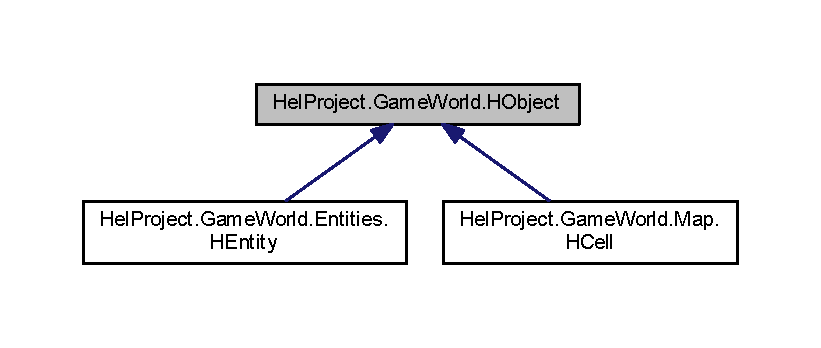
\includegraphics[width=350pt]{class_hel_project_1_1_game_world_1_1_h_object__inherit__graph}
\end{center}
\end{figure}
\subsection*{Public Member Functions}
\begin{DoxyCompactItemize}
\item 
\hyperlink{class_hel_project_1_1_game_world_1_1_h_object_ac10ea2725a0721b3f60d8e04bc89eda5}{H\+Object} ()
\begin{DoxyCompactList}\small\item\em Creates an object \end{DoxyCompactList}\item 
\hyperlink{class_hel_project_1_1_game_world_1_1_h_object_a4c6d74d0ac6cabce471ddc176bc20321}{H\+Object} (Vector2 position)
\begin{DoxyCompactList}\small\item\em Creates an object \end{DoxyCompactList}\item 
\hyperlink{class_hel_project_1_1_game_world_1_1_h_object_a8717f6ef86d820de6ab113b516ef039f}{H\+Object} (bool is\+Walkable, Vector2 position)
\begin{DoxyCompactList}\small\item\em Creates an object \end{DoxyCompactList}\item 
virtual void \hyperlink{class_hel_project_1_1_game_world_1_1_h_object_a2de39710b20f7af4e1e2463ca93656f8}{Load\+Content} ()
\begin{DoxyCompactList}\small\item\em Override this to load content \end{DoxyCompactList}\item 
virtual void \hyperlink{class_hel_project_1_1_game_world_1_1_h_object_a30efa177423e89a85e45b76fe35d6724}{Unload\+Content} ()
\begin{DoxyCompactList}\small\item\em Override this to unload content \end{DoxyCompactList}\item 
virtual void \hyperlink{class_hel_project_1_1_game_world_1_1_h_object_a2e4ba3d334e48c9b74cc1b2b821f030b}{Update} (Game\+Time game\+Time)
\begin{DoxyCompactList}\small\item\em Override this to update object \end{DoxyCompactList}\item 
virtual void \hyperlink{class_hel_project_1_1_game_world_1_1_h_object_aa48c9288756739f80a59bdf6f4fe7f3f}{Draw} (Sprite\+Batch sprite\+Batch)
\begin{DoxyCompactList}\small\item\em Override this to draw object \end{DoxyCompactList}\end{DoxyCompactItemize}
\subsection*{Protected Attributes}
\begin{DoxyCompactItemize}
\item 
\hypertarget{class_hel_project_1_1_game_world_1_1_h_object_aa48be7d1041c9417c831a904bd52377f}{}const bool {\bfseries D\+E\+F\+A\+U\+L\+T\+\_\+\+I\+S\+\_\+\+W\+A\+L\+K\+A\+B\+L\+E\+\_\+\+V\+A\+L\+U\+E} = false\label{class_hel_project_1_1_game_world_1_1_h_object_aa48be7d1041c9417c831a904bd52377f}

\item 
\hypertarget{class_hel_project_1_1_game_world_1_1_h_object_a32e043831c6f30e1a73ee033f9d00483}{}const float {\bfseries D\+E\+F\+A\+U\+L\+T\+\_\+\+P\+O\+S\+I\+T\+I\+O\+N\+\_\+\+X\+\_\+\+V\+A\+L\+U\+E} = 0.\+0f\label{class_hel_project_1_1_game_world_1_1_h_object_a32e043831c6f30e1a73ee033f9d00483}

\item 
\hypertarget{class_hel_project_1_1_game_world_1_1_h_object_a5b601f5ab506ca13d2f27ec8d0bd0540}{}const float {\bfseries D\+E\+F\+A\+U\+L\+T\+\_\+\+P\+O\+S\+I\+T\+I\+O\+N\+\_\+\+Y\+\_\+\+V\+A\+L\+U\+E} = 0.\+0f\label{class_hel_project_1_1_game_world_1_1_h_object_a5b601f5ab506ca13d2f27ec8d0bd0540}

\end{DoxyCompactItemize}
\subsection*{Properties}
\begin{DoxyCompactItemize}
\item 
Vector2 \hyperlink{class_hel_project_1_1_game_world_1_1_h_object_af5297b9bdeac2d179b0bee66ff111f94}{Position}\hspace{0.3cm}{\ttfamily  \mbox{[}get, set\mbox{]}}
\begin{DoxyCompactList}\small\item\em Position of the entity \end{DoxyCompactList}\item 
bool \hyperlink{class_hel_project_1_1_game_world_1_1_h_object_a97444e657db0148fb442570fbd7fe98f}{Is\+Walkable}\hspace{0.3cm}{\ttfamily  \mbox{[}get, set\mbox{]}}
\begin{DoxyCompactList}\small\item\em Can be walked by entities \end{DoxyCompactList}\end{DoxyCompactItemize}


\subsection{Detailed Description}
Abstract class for all entities of the game 



\subsection{Constructor \& Destructor Documentation}
\hypertarget{class_hel_project_1_1_game_world_1_1_h_object_ac10ea2725a0721b3f60d8e04bc89eda5}{}\index{Hel\+Project\+::\+Game\+World\+::\+H\+Object@{Hel\+Project\+::\+Game\+World\+::\+H\+Object}!H\+Object@{H\+Object}}
\index{H\+Object@{H\+Object}!Hel\+Project\+::\+Game\+World\+::\+H\+Object@{Hel\+Project\+::\+Game\+World\+::\+H\+Object}}
\subsubsection[{H\+Object}]{\setlength{\rightskip}{0pt plus 5cm}Hel\+Project.\+Game\+World.\+H\+Object.\+H\+Object (
\begin{DoxyParamCaption}
{}
\end{DoxyParamCaption}
)}\label{class_hel_project_1_1_game_world_1_1_h_object_ac10ea2725a0721b3f60d8e04bc89eda5}


Creates an object 

\hypertarget{class_hel_project_1_1_game_world_1_1_h_object_a4c6d74d0ac6cabce471ddc176bc20321}{}\index{Hel\+Project\+::\+Game\+World\+::\+H\+Object@{Hel\+Project\+::\+Game\+World\+::\+H\+Object}!H\+Object@{H\+Object}}
\index{H\+Object@{H\+Object}!Hel\+Project\+::\+Game\+World\+::\+H\+Object@{Hel\+Project\+::\+Game\+World\+::\+H\+Object}}
\subsubsection[{H\+Object}]{\setlength{\rightskip}{0pt plus 5cm}Hel\+Project.\+Game\+World.\+H\+Object.\+H\+Object (
\begin{DoxyParamCaption}
\item[{Vector2}]{position}
\end{DoxyParamCaption}
)}\label{class_hel_project_1_1_game_world_1_1_h_object_a4c6d74d0ac6cabce471ddc176bc20321}


Creates an object 


\begin{DoxyParams}{Parameters}
{\em position} & Position of the object\\
\hline
\end{DoxyParams}
\hypertarget{class_hel_project_1_1_game_world_1_1_h_object_a8717f6ef86d820de6ab113b516ef039f}{}\index{Hel\+Project\+::\+Game\+World\+::\+H\+Object@{Hel\+Project\+::\+Game\+World\+::\+H\+Object}!H\+Object@{H\+Object}}
\index{H\+Object@{H\+Object}!Hel\+Project\+::\+Game\+World\+::\+H\+Object@{Hel\+Project\+::\+Game\+World\+::\+H\+Object}}
\subsubsection[{H\+Object}]{\setlength{\rightskip}{0pt plus 5cm}Hel\+Project.\+Game\+World.\+H\+Object.\+H\+Object (
\begin{DoxyParamCaption}
\item[{bool}]{is\+Walkable, }
\item[{Vector2}]{position}
\end{DoxyParamCaption}
)}\label{class_hel_project_1_1_game_world_1_1_h_object_a8717f6ef86d820de6ab113b516ef039f}


Creates an object 


\begin{DoxyParams}{Parameters}
{\em is\+Walkable} & Can the object be \textquotesingle{}walked\textquotesingle{} on by entities\\
\hline
{\em position} & Position of the object\\
\hline
\end{DoxyParams}


\subsection{Member Function Documentation}
\hypertarget{class_hel_project_1_1_game_world_1_1_h_object_aa48c9288756739f80a59bdf6f4fe7f3f}{}\index{Hel\+Project\+::\+Game\+World\+::\+H\+Object@{Hel\+Project\+::\+Game\+World\+::\+H\+Object}!Draw@{Draw}}
\index{Draw@{Draw}!Hel\+Project\+::\+Game\+World\+::\+H\+Object@{Hel\+Project\+::\+Game\+World\+::\+H\+Object}}
\subsubsection[{Draw}]{\setlength{\rightskip}{0pt plus 5cm}virtual void Hel\+Project.\+Game\+World.\+H\+Object.\+Draw (
\begin{DoxyParamCaption}
\item[{Sprite\+Batch}]{sprite\+Batch}
\end{DoxyParamCaption}
)\hspace{0.3cm}{\ttfamily [virtual]}}\label{class_hel_project_1_1_game_world_1_1_h_object_aa48c9288756739f80a59bdf6f4fe7f3f}


Override this to draw object 


\begin{DoxyParams}{Parameters}
{\em sprite\+Batch} & \\
\hline
\end{DoxyParams}


Reimplemented in \hyperlink{class_hel_project_1_1_game_world_1_1_entities_1_1_h_entity_aac4efdcaa42e096838556aba9345f8d5}{Hel\+Project.\+Game\+World.\+Entities.\+H\+Entity}, \hyperlink{class_hel_project_1_1_game_world_1_1_h_item_a463357f63d56ec3ac4836a224c179892}{Hel\+Project.\+Game\+World.\+H\+Item}, \hyperlink{class_hel_project_1_1_game_world_1_1_entities_1_1_h_hero_a8a08422c569dbff045d597aa1663c338}{Hel\+Project.\+Game\+World.\+Entities.\+H\+Hero}, and \hyperlink{class_hel_project_1_1_game_world_1_1_entities_1_1_h_hostile_a548b6f33addf42cbe85d4058ace51d76}{Hel\+Project.\+Game\+World.\+Entities.\+H\+Hostile}.

\hypertarget{class_hel_project_1_1_game_world_1_1_h_object_a2de39710b20f7af4e1e2463ca93656f8}{}\index{Hel\+Project\+::\+Game\+World\+::\+H\+Object@{Hel\+Project\+::\+Game\+World\+::\+H\+Object}!Load\+Content@{Load\+Content}}
\index{Load\+Content@{Load\+Content}!Hel\+Project\+::\+Game\+World\+::\+H\+Object@{Hel\+Project\+::\+Game\+World\+::\+H\+Object}}
\subsubsection[{Load\+Content}]{\setlength{\rightskip}{0pt plus 5cm}virtual void Hel\+Project.\+Game\+World.\+H\+Object.\+Load\+Content (
\begin{DoxyParamCaption}
{}
\end{DoxyParamCaption}
)\hspace{0.3cm}{\ttfamily [virtual]}}\label{class_hel_project_1_1_game_world_1_1_h_object_a2de39710b20f7af4e1e2463ca93656f8}


Override this to load content 



Reimplemented in \hyperlink{class_hel_project_1_1_game_world_1_1_entities_1_1_h_hostile_ab244ce132ea02c1e4bf9e38f199dbe85}{Hel\+Project.\+Game\+World.\+Entities.\+H\+Hostile}, and \hyperlink{class_hel_project_1_1_game_world_1_1_entities_1_1_h_hero_a8b69c5d3b4e7c68b2472de1d3bf76618}{Hel\+Project.\+Game\+World.\+Entities.\+H\+Hero}.

\hypertarget{class_hel_project_1_1_game_world_1_1_h_object_a30efa177423e89a85e45b76fe35d6724}{}\index{Hel\+Project\+::\+Game\+World\+::\+H\+Object@{Hel\+Project\+::\+Game\+World\+::\+H\+Object}!Unload\+Content@{Unload\+Content}}
\index{Unload\+Content@{Unload\+Content}!Hel\+Project\+::\+Game\+World\+::\+H\+Object@{Hel\+Project\+::\+Game\+World\+::\+H\+Object}}
\subsubsection[{Unload\+Content}]{\setlength{\rightskip}{0pt plus 5cm}virtual void Hel\+Project.\+Game\+World.\+H\+Object.\+Unload\+Content (
\begin{DoxyParamCaption}
{}
\end{DoxyParamCaption}
)\hspace{0.3cm}{\ttfamily [virtual]}}\label{class_hel_project_1_1_game_world_1_1_h_object_a30efa177423e89a85e45b76fe35d6724}


Override this to unload content 



Reimplemented in \hyperlink{class_hel_project_1_1_game_world_1_1_entities_1_1_h_hero_a2e665a9cc2a0fea82c4ac7c8b1f3468b}{Hel\+Project.\+Game\+World.\+Entities.\+H\+Hero}, and \hyperlink{class_hel_project_1_1_game_world_1_1_entities_1_1_h_hostile_a43c15c63adde7e4bb5747625a40789d7}{Hel\+Project.\+Game\+World.\+Entities.\+H\+Hostile}.

\hypertarget{class_hel_project_1_1_game_world_1_1_h_object_a2e4ba3d334e48c9b74cc1b2b821f030b}{}\index{Hel\+Project\+::\+Game\+World\+::\+H\+Object@{Hel\+Project\+::\+Game\+World\+::\+H\+Object}!Update@{Update}}
\index{Update@{Update}!Hel\+Project\+::\+Game\+World\+::\+H\+Object@{Hel\+Project\+::\+Game\+World\+::\+H\+Object}}
\subsubsection[{Update}]{\setlength{\rightskip}{0pt plus 5cm}virtual void Hel\+Project.\+Game\+World.\+H\+Object.\+Update (
\begin{DoxyParamCaption}
\item[{Game\+Time}]{game\+Time}
\end{DoxyParamCaption}
)\hspace{0.3cm}{\ttfamily [virtual]}}\label{class_hel_project_1_1_game_world_1_1_h_object_a2e4ba3d334e48c9b74cc1b2b821f030b}


Override this to update object 


\begin{DoxyParams}{Parameters}
{\em game\+Time} & \\
\hline
\end{DoxyParams}


Reimplemented in \hyperlink{class_hel_project_1_1_game_world_1_1_entities_1_1_h_entity_a3feda059e3ebd1a20579260a6dc60291}{Hel\+Project.\+Game\+World.\+Entities.\+H\+Entity}, \hyperlink{class_hel_project_1_1_game_world_1_1_entities_1_1_h_hero_a421c030a8fde6fe6707b5416d0db46ff}{Hel\+Project.\+Game\+World.\+Entities.\+H\+Hero}, and \hyperlink{class_hel_project_1_1_game_world_1_1_entities_1_1_h_hostile_a3ce954aa41e47c306487d94ba64ae822}{Hel\+Project.\+Game\+World.\+Entities.\+H\+Hostile}.



\subsection{Property Documentation}
\hypertarget{class_hel_project_1_1_game_world_1_1_h_object_a97444e657db0148fb442570fbd7fe98f}{}\index{Hel\+Project\+::\+Game\+World\+::\+H\+Object@{Hel\+Project\+::\+Game\+World\+::\+H\+Object}!Is\+Walkable@{Is\+Walkable}}
\index{Is\+Walkable@{Is\+Walkable}!Hel\+Project\+::\+Game\+World\+::\+H\+Object@{Hel\+Project\+::\+Game\+World\+::\+H\+Object}}
\subsubsection[{Is\+Walkable}]{\setlength{\rightskip}{0pt plus 5cm}bool Hel\+Project.\+Game\+World.\+H\+Object.\+Is\+Walkable\hspace{0.3cm}{\ttfamily [get]}, {\ttfamily [set]}}\label{class_hel_project_1_1_game_world_1_1_h_object_a97444e657db0148fb442570fbd7fe98f}


Can be walked by entities 

\hypertarget{class_hel_project_1_1_game_world_1_1_h_object_af5297b9bdeac2d179b0bee66ff111f94}{}\index{Hel\+Project\+::\+Game\+World\+::\+H\+Object@{Hel\+Project\+::\+Game\+World\+::\+H\+Object}!Position@{Position}}
\index{Position@{Position}!Hel\+Project\+::\+Game\+World\+::\+H\+Object@{Hel\+Project\+::\+Game\+World\+::\+H\+Object}}
\subsubsection[{Position}]{\setlength{\rightskip}{0pt plus 5cm}Vector2 Hel\+Project.\+Game\+World.\+H\+Object.\+Position\hspace{0.3cm}{\ttfamily [get]}, {\ttfamily [set]}}\label{class_hel_project_1_1_game_world_1_1_h_object_af5297b9bdeac2d179b0bee66ff111f94}


Position of the entity 



The documentation for this class was generated from the following file\+:\begin{DoxyCompactItemize}
\item 
src/\+Hel\+Project/\+Game\+World/H\+Object.\+cs\end{DoxyCompactItemize}

\hypertarget{class_hel_project_1_1_game_world_1_1_spells_1_1_h_spell}{}\section{Hel\+Project.\+Game\+World.\+Spells.\+H\+Spell Class Reference}
\label{class_hel_project_1_1_game_world_1_1_spells_1_1_h_spell}\index{Hel\+Project.\+Game\+World.\+Spells.\+H\+Spell@{Hel\+Project.\+Game\+World.\+Spells.\+H\+Spell}}


Spell of the game  




Inheritance diagram for Hel\+Project.\+Game\+World.\+Spells.\+H\+Spell\+:
% FIG 0
\subsection*{Public Member Functions}
\begin{DoxyCompactItemize}
\item 
\hyperlink{class_hel_project_1_1_game_world_1_1_spells_1_1_h_spell_a0320952c7e7ed4bda12288dc6f9e0f62}{H\+Spell} (\hyperlink{class_hel_project_1_1_game_world_1_1_entities_1_1_h_hero}{H\+Hero} hero, \hyperlink{class_hel_project_1_1_features_1_1_feature_collection}{Feature\+Collection} features, float time\+Of\+Effect, string name)
\begin{DoxyCompactList}\small\item\em Creates a spell \end{DoxyCompactList}\item 
virtual void \hyperlink{class_hel_project_1_1_game_world_1_1_spells_1_1_h_spell_a2c30200e62a6a938156035098a9c6a1f}{Load\+Content} ()
\begin{DoxyCompactList}\small\item\em Loads the content of the spell \end{DoxyCompactList}\item 
virtual void \hyperlink{class_hel_project_1_1_game_world_1_1_spells_1_1_h_spell_a760e3d340c43f234465d07e2782e3e3a}{Unload\+Content} ()
\begin{DoxyCompactList}\small\item\em Unloads the content of the spell \end{DoxyCompactList}\item 
virtual void \hyperlink{class_hel_project_1_1_game_world_1_1_spells_1_1_h_spell_a19c9c7c407b20861184ef8538614142b}{Update} (Game\+Time game\+Time)
\begin{DoxyCompactList}\small\item\em Updates the spell in the game loop \end{DoxyCompactList}\item 
virtual void \hyperlink{class_hel_project_1_1_game_world_1_1_spells_1_1_h_spell_a71cfca2b0bd3d7bcc91d8fae7180a21f}{Draw} (Sprite\+Batch sprite\+Batch)
\begin{DoxyCompactList}\small\item\em Draws the spell \end{DoxyCompactList}\end{DoxyCompactItemize}
\subsection*{Properties}
\begin{DoxyCompactItemize}
\item 
\hyperlink{class_hel_project_1_1_game_world_1_1_entities_1_1_h_hero}{H\+Hero} \hyperlink{class_hel_project_1_1_game_world_1_1_spells_1_1_h_spell_a1867f356bf0a68b755703db7e556cbbd}{Hero}\hspace{0.3cm}{\ttfamily  \mbox{[}get, set\mbox{]}}
\begin{DoxyCompactList}\small\item\em Hero that the spell is attached to \end{DoxyCompactList}\item 
\hyperlink{class_hel_project_1_1_features_1_1_feature_collection}{Feature\+Collection} \hyperlink{class_hel_project_1_1_game_world_1_1_spells_1_1_h_spell_a404a775604d84ff622ecc2a72cf5f91a}{Features}\hspace{0.3cm}{\ttfamily  \mbox{[}get, set\mbox{]}}
\begin{DoxyCompactList}\small\item\em \hyperlink{namespace_hel_project_1_1_features}{Features} of the spell \end{DoxyCompactList}\item 
string \hyperlink{class_hel_project_1_1_game_world_1_1_spells_1_1_h_spell_a66d41a1b498d10e9d77229bdb39fd783}{Name}\hspace{0.3cm}{\ttfamily  \mbox{[}get, set\mbox{]}}
\begin{DoxyCompactList}\small\item\em Name of the spell \end{DoxyCompactList}\item 
float \hyperlink{class_hel_project_1_1_game_world_1_1_spells_1_1_h_spell_ae6cb50ade7feb332679ed6b45079d1ce}{Time\+Of\+Effect}\hspace{0.3cm}{\ttfamily  \mbox{[}get, set\mbox{]}}
\begin{DoxyCompactList}\small\item\em Time of effect once the spell is active \end{DoxyCompactList}\end{DoxyCompactItemize}


\subsection{Detailed Description}
Spell of the game 



\subsection{Constructor \& Destructor Documentation}
\hypertarget{class_hel_project_1_1_game_world_1_1_spells_1_1_h_spell_a0320952c7e7ed4bda12288dc6f9e0f62}{}\index{Hel\+Project\+::\+Game\+World\+::\+Spells\+::\+H\+Spell@{Hel\+Project\+::\+Game\+World\+::\+Spells\+::\+H\+Spell}!H\+Spell@{H\+Spell}}
\index{H\+Spell@{H\+Spell}!Hel\+Project\+::\+Game\+World\+::\+Spells\+::\+H\+Spell@{Hel\+Project\+::\+Game\+World\+::\+Spells\+::\+H\+Spell}}
\subsubsection[{H\+Spell}]{\setlength{\rightskip}{0pt plus 5cm}Hel\+Project.\+Game\+World.\+Spells.\+H\+Spell.\+H\+Spell (
\begin{DoxyParamCaption}
\item[{{\bf H\+Hero}}]{hero, }
\item[{{\bf Feature\+Collection}}]{features, }
\item[{float}]{time\+Of\+Effect, }
\item[{string}]{name}
\end{DoxyParamCaption}
)}\label{class_hel_project_1_1_game_world_1_1_spells_1_1_h_spell_a0320952c7e7ed4bda12288dc6f9e0f62}


Creates a spell 


\begin{DoxyParams}{Parameters}
{\em hero} & Hero that the spell is attached to\\
\hline
{\em features} & \hyperlink{namespace_hel_project_1_1_features}{Features} of the spell\\
\hline
{\em time\+Of\+Effect} & Time of effect once the spell is active\\
\hline
{\em name} & Name of the spell\\
\hline
\end{DoxyParams}


\subsection{Member Function Documentation}
\hypertarget{class_hel_project_1_1_game_world_1_1_spells_1_1_h_spell_a71cfca2b0bd3d7bcc91d8fae7180a21f}{}\index{Hel\+Project\+::\+Game\+World\+::\+Spells\+::\+H\+Spell@{Hel\+Project\+::\+Game\+World\+::\+Spells\+::\+H\+Spell}!Draw@{Draw}}
\index{Draw@{Draw}!Hel\+Project\+::\+Game\+World\+::\+Spells\+::\+H\+Spell@{Hel\+Project\+::\+Game\+World\+::\+Spells\+::\+H\+Spell}}
\subsubsection[{Draw}]{\setlength{\rightskip}{0pt plus 5cm}virtual void Hel\+Project.\+Game\+World.\+Spells.\+H\+Spell.\+Draw (
\begin{DoxyParamCaption}
\item[{Sprite\+Batch}]{sprite\+Batch}
\end{DoxyParamCaption}
)\hspace{0.3cm}{\ttfamily [virtual]}}\label{class_hel_project_1_1_game_world_1_1_spells_1_1_h_spell_a71cfca2b0bd3d7bcc91d8fae7180a21f}


Draws the spell 


\begin{DoxyParams}{Parameters}
{\em sprite\+Batch} & \\
\hline
\end{DoxyParams}
\hypertarget{class_hel_project_1_1_game_world_1_1_spells_1_1_h_spell_a2c30200e62a6a938156035098a9c6a1f}{}\index{Hel\+Project\+::\+Game\+World\+::\+Spells\+::\+H\+Spell@{Hel\+Project\+::\+Game\+World\+::\+Spells\+::\+H\+Spell}!Load\+Content@{Load\+Content}}
\index{Load\+Content@{Load\+Content}!Hel\+Project\+::\+Game\+World\+::\+Spells\+::\+H\+Spell@{Hel\+Project\+::\+Game\+World\+::\+Spells\+::\+H\+Spell}}
\subsubsection[{Load\+Content}]{\setlength{\rightskip}{0pt plus 5cm}virtual void Hel\+Project.\+Game\+World.\+Spells.\+H\+Spell.\+Load\+Content (
\begin{DoxyParamCaption}
{}
\end{DoxyParamCaption}
)\hspace{0.3cm}{\ttfamily [virtual]}}\label{class_hel_project_1_1_game_world_1_1_spells_1_1_h_spell_a2c30200e62a6a938156035098a9c6a1f}


Loads the content of the spell 

\hypertarget{class_hel_project_1_1_game_world_1_1_spells_1_1_h_spell_a760e3d340c43f234465d07e2782e3e3a}{}\index{Hel\+Project\+::\+Game\+World\+::\+Spells\+::\+H\+Spell@{Hel\+Project\+::\+Game\+World\+::\+Spells\+::\+H\+Spell}!Unload\+Content@{Unload\+Content}}
\index{Unload\+Content@{Unload\+Content}!Hel\+Project\+::\+Game\+World\+::\+Spells\+::\+H\+Spell@{Hel\+Project\+::\+Game\+World\+::\+Spells\+::\+H\+Spell}}
\subsubsection[{Unload\+Content}]{\setlength{\rightskip}{0pt plus 5cm}virtual void Hel\+Project.\+Game\+World.\+Spells.\+H\+Spell.\+Unload\+Content (
\begin{DoxyParamCaption}
{}
\end{DoxyParamCaption}
)\hspace{0.3cm}{\ttfamily [virtual]}}\label{class_hel_project_1_1_game_world_1_1_spells_1_1_h_spell_a760e3d340c43f234465d07e2782e3e3a}


Unloads the content of the spell 

\hypertarget{class_hel_project_1_1_game_world_1_1_spells_1_1_h_spell_a19c9c7c407b20861184ef8538614142b}{}\index{Hel\+Project\+::\+Game\+World\+::\+Spells\+::\+H\+Spell@{Hel\+Project\+::\+Game\+World\+::\+Spells\+::\+H\+Spell}!Update@{Update}}
\index{Update@{Update}!Hel\+Project\+::\+Game\+World\+::\+Spells\+::\+H\+Spell@{Hel\+Project\+::\+Game\+World\+::\+Spells\+::\+H\+Spell}}
\subsubsection[{Update}]{\setlength{\rightskip}{0pt plus 5cm}virtual void Hel\+Project.\+Game\+World.\+Spells.\+H\+Spell.\+Update (
\begin{DoxyParamCaption}
\item[{Game\+Time}]{game\+Time}
\end{DoxyParamCaption}
)\hspace{0.3cm}{\ttfamily [virtual]}}\label{class_hel_project_1_1_game_world_1_1_spells_1_1_h_spell_a19c9c7c407b20861184ef8538614142b}


Updates the spell in the game loop 


\begin{DoxyParams}{Parameters}
{\em game\+Time} & \\
\hline
\end{DoxyParams}


\subsection{Property Documentation}
\hypertarget{class_hel_project_1_1_game_world_1_1_spells_1_1_h_spell_a404a775604d84ff622ecc2a72cf5f91a}{}\index{Hel\+Project\+::\+Game\+World\+::\+Spells\+::\+H\+Spell@{Hel\+Project\+::\+Game\+World\+::\+Spells\+::\+H\+Spell}!Features@{Features}}
\index{Features@{Features}!Hel\+Project\+::\+Game\+World\+::\+Spells\+::\+H\+Spell@{Hel\+Project\+::\+Game\+World\+::\+Spells\+::\+H\+Spell}}
\subsubsection[{Features}]{\setlength{\rightskip}{0pt plus 5cm}{\bf Feature\+Collection} Hel\+Project.\+Game\+World.\+Spells.\+H\+Spell.\+Features\hspace{0.3cm}{\ttfamily [get]}, {\ttfamily [set]}}\label{class_hel_project_1_1_game_world_1_1_spells_1_1_h_spell_a404a775604d84ff622ecc2a72cf5f91a}


\hyperlink{namespace_hel_project_1_1_features}{Features} of the spell 

\hypertarget{class_hel_project_1_1_game_world_1_1_spells_1_1_h_spell_a1867f356bf0a68b755703db7e556cbbd}{}\index{Hel\+Project\+::\+Game\+World\+::\+Spells\+::\+H\+Spell@{Hel\+Project\+::\+Game\+World\+::\+Spells\+::\+H\+Spell}!Hero@{Hero}}
\index{Hero@{Hero}!Hel\+Project\+::\+Game\+World\+::\+Spells\+::\+H\+Spell@{Hel\+Project\+::\+Game\+World\+::\+Spells\+::\+H\+Spell}}
\subsubsection[{Hero}]{\setlength{\rightskip}{0pt plus 5cm}{\bf H\+Hero} Hel\+Project.\+Game\+World.\+Spells.\+H\+Spell.\+Hero\hspace{0.3cm}{\ttfamily [get]}, {\ttfamily [set]}}\label{class_hel_project_1_1_game_world_1_1_spells_1_1_h_spell_a1867f356bf0a68b755703db7e556cbbd}


Hero that the spell is attached to 

\hypertarget{class_hel_project_1_1_game_world_1_1_spells_1_1_h_spell_a66d41a1b498d10e9d77229bdb39fd783}{}\index{Hel\+Project\+::\+Game\+World\+::\+Spells\+::\+H\+Spell@{Hel\+Project\+::\+Game\+World\+::\+Spells\+::\+H\+Spell}!Name@{Name}}
\index{Name@{Name}!Hel\+Project\+::\+Game\+World\+::\+Spells\+::\+H\+Spell@{Hel\+Project\+::\+Game\+World\+::\+Spells\+::\+H\+Spell}}
\subsubsection[{Name}]{\setlength{\rightskip}{0pt plus 5cm}string Hel\+Project.\+Game\+World.\+Spells.\+H\+Spell.\+Name\hspace{0.3cm}{\ttfamily [get]}, {\ttfamily [set]}}\label{class_hel_project_1_1_game_world_1_1_spells_1_1_h_spell_a66d41a1b498d10e9d77229bdb39fd783}


Name of the spell 

\hypertarget{class_hel_project_1_1_game_world_1_1_spells_1_1_h_spell_ae6cb50ade7feb332679ed6b45079d1ce}{}\index{Hel\+Project\+::\+Game\+World\+::\+Spells\+::\+H\+Spell@{Hel\+Project\+::\+Game\+World\+::\+Spells\+::\+H\+Spell}!Time\+Of\+Effect@{Time\+Of\+Effect}}
\index{Time\+Of\+Effect@{Time\+Of\+Effect}!Hel\+Project\+::\+Game\+World\+::\+Spells\+::\+H\+Spell@{Hel\+Project\+::\+Game\+World\+::\+Spells\+::\+H\+Spell}}
\subsubsection[{Time\+Of\+Effect}]{\setlength{\rightskip}{0pt plus 5cm}float Hel\+Project.\+Game\+World.\+Spells.\+H\+Spell.\+Time\+Of\+Effect\hspace{0.3cm}{\ttfamily [get]}, {\ttfamily [set]}}\label{class_hel_project_1_1_game_world_1_1_spells_1_1_h_spell_ae6cb50ade7feb332679ed6b45079d1ce}


Time of effect once the spell is active 



The documentation for this class was generated from the following file\+:\begin{DoxyCompactItemize}
\item 
src/\+Hel\+Project/\+Game\+World/\+Spells/H\+Spell.\+cs\end{DoxyCompactItemize}

\hypertarget{class_hel_project_1_1_game_world_1_1_spells_1_1_h_spell_buff}{}\section{Hel\+Project.\+Game\+World.\+Spells.\+H\+Spell\+Buff Class Reference}
\label{class_hel_project_1_1_game_world_1_1_spells_1_1_h_spell_buff}\index{Hel\+Project.\+Game\+World.\+Spells.\+H\+Spell\+Buff@{Hel\+Project.\+Game\+World.\+Spells.\+H\+Spell\+Buff}}


Spell buff  




Inheritance diagram for Hel\+Project.\+Game\+World.\+Spells.\+H\+Spell\+Buff\+:
% FIG 0


Collaboration diagram for Hel\+Project.\+Game\+World.\+Spells.\+H\+Spell\+Buff\+:
% FIG 1
\subsection*{Public Member Functions}
\begin{DoxyCompactItemize}
\item 
\hyperlink{class_hel_project_1_1_game_world_1_1_spells_1_1_h_spell_buff_ad751033489b43b527b0f1c4bacf166b4}{H\+Spell\+Buff} (\hyperlink{class_hel_project_1_1_game_world_1_1_entities_1_1_h_hero}{H\+Hero} hero, \hyperlink{class_hel_project_1_1_features_1_1_feature_collection}{Feature\+Collection} features, float time\+Of\+Effect, string name)
\begin{DoxyCompactList}\small\item\em Creates a spell buff \end{DoxyCompactList}\end{DoxyCompactItemize}
\subsection*{Additional Inherited Members}


\subsection{Detailed Description}
Spell buff 



\subsection{Constructor \& Destructor Documentation}
\hypertarget{class_hel_project_1_1_game_world_1_1_spells_1_1_h_spell_buff_ad751033489b43b527b0f1c4bacf166b4}{}\index{Hel\+Project\+::\+Game\+World\+::\+Spells\+::\+H\+Spell\+Buff@{Hel\+Project\+::\+Game\+World\+::\+Spells\+::\+H\+Spell\+Buff}!H\+Spell\+Buff@{H\+Spell\+Buff}}
\index{H\+Spell\+Buff@{H\+Spell\+Buff}!Hel\+Project\+::\+Game\+World\+::\+Spells\+::\+H\+Spell\+Buff@{Hel\+Project\+::\+Game\+World\+::\+Spells\+::\+H\+Spell\+Buff}}
\subsubsection[{H\+Spell\+Buff}]{\setlength{\rightskip}{0pt plus 5cm}Hel\+Project.\+Game\+World.\+Spells.\+H\+Spell\+Buff.\+H\+Spell\+Buff (
\begin{DoxyParamCaption}
\item[{{\bf H\+Hero}}]{hero, }
\item[{{\bf Feature\+Collection}}]{features, }
\item[{float}]{time\+Of\+Effect, }
\item[{string}]{name}
\end{DoxyParamCaption}
)}\label{class_hel_project_1_1_game_world_1_1_spells_1_1_h_spell_buff_ad751033489b43b527b0f1c4bacf166b4}


Creates a spell buff 


\begin{DoxyParams}{Parameters}
{\em hero} & Hero that the spell is attached to\\
\hline
{\em features} & \hyperlink{namespace_hel_project_1_1_features}{Features} of the spell\\
\hline
{\em time\+Of\+Effect} & Time of effect once the spell is active\\
\hline
{\em name} & Name of the spell\\
\hline
\end{DoxyParams}


The documentation for this class was generated from the following file\+:\begin{DoxyCompactItemize}
\item 
src/\+Hel\+Project/\+Game\+World/\+Spells/H\+Spell\+Buff.\+cs\end{DoxyCompactItemize}

\hypertarget{class_hel_project_1_1_game_world_1_1_spells_1_1_h_spell_single_target}{}\section{Hel\+Project.\+Game\+World.\+Spells.\+H\+Spell\+Single\+Target Class Reference}
\label{class_hel_project_1_1_game_world_1_1_spells_1_1_h_spell_single_target}\index{Hel\+Project.\+Game\+World.\+Spells.\+H\+Spell\+Single\+Target@{Hel\+Project.\+Game\+World.\+Spells.\+H\+Spell\+Single\+Target}}


Single targeted spell  




Inheritance diagram for Hel\+Project.\+Game\+World.\+Spells.\+H\+Spell\+Single\+Target\+:
% FIG 0


Collaboration diagram for Hel\+Project.\+Game\+World.\+Spells.\+H\+Spell\+Single\+Target\+:
% FIG 1
\subsection*{Public Member Functions}
\begin{DoxyCompactItemize}
\item 
\hyperlink{class_hel_project_1_1_game_world_1_1_spells_1_1_h_spell_single_target_ac17216b17a63c040afc7dae6a14f420a}{H\+Spell\+Single\+Target} (\hyperlink{class_hel_project_1_1_game_world_1_1_entities_1_1_h_hero}{H\+Hero} hero, \hyperlink{class_hel_project_1_1_features_1_1_feature_collection}{Feature\+Collection} features, float time\+Of\+Effect, string name, \hyperlink{class_hel_project_1_1_game_world_1_1_entities_1_1_h_entity}{H\+Entity} target)
\begin{DoxyCompactList}\small\item\em Creates a single target spell \end{DoxyCompactList}\end{DoxyCompactItemize}
\subsection*{Properties}
\begin{DoxyCompactItemize}
\item 
\hyperlink{class_hel_project_1_1_game_world_1_1_entities_1_1_h_entity}{H\+Entity} \hyperlink{class_hel_project_1_1_game_world_1_1_spells_1_1_h_spell_single_target_addb117babce01c6786178be3d38c3222}{Target}\hspace{0.3cm}{\ttfamily  \mbox{[}get, set\mbox{]}}
\begin{DoxyCompactList}\small\item\em Target of the spell \end{DoxyCompactList}\end{DoxyCompactItemize}


\subsection{Detailed Description}
Single targeted spell 



\subsection{Constructor \& Destructor Documentation}
\hypertarget{class_hel_project_1_1_game_world_1_1_spells_1_1_h_spell_single_target_ac17216b17a63c040afc7dae6a14f420a}{}\index{Hel\+Project\+::\+Game\+World\+::\+Spells\+::\+H\+Spell\+Single\+Target@{Hel\+Project\+::\+Game\+World\+::\+Spells\+::\+H\+Spell\+Single\+Target}!H\+Spell\+Single\+Target@{H\+Spell\+Single\+Target}}
\index{H\+Spell\+Single\+Target@{H\+Spell\+Single\+Target}!Hel\+Project\+::\+Game\+World\+::\+Spells\+::\+H\+Spell\+Single\+Target@{Hel\+Project\+::\+Game\+World\+::\+Spells\+::\+H\+Spell\+Single\+Target}}
\subsubsection[{H\+Spell\+Single\+Target}]{\setlength{\rightskip}{0pt plus 5cm}Hel\+Project.\+Game\+World.\+Spells.\+H\+Spell\+Single\+Target.\+H\+Spell\+Single\+Target (
\begin{DoxyParamCaption}
\item[{{\bf H\+Hero}}]{hero, }
\item[{{\bf Feature\+Collection}}]{features, }
\item[{float}]{time\+Of\+Effect, }
\item[{string}]{name, }
\item[{{\bf H\+Entity}}]{target}
\end{DoxyParamCaption}
)}\label{class_hel_project_1_1_game_world_1_1_spells_1_1_h_spell_single_target_ac17216b17a63c040afc7dae6a14f420a}


Creates a single target spell 


\begin{DoxyParams}{Parameters}
{\em hero} & Hero that the spell is attached to\\
\hline
{\em features} & \hyperlink{namespace_hel_project_1_1_features}{Features} of the spell\\
\hline
{\em time\+Of\+Effect} & Time of effect once the spell is active\\
\hline
{\em name} & Name of the spell\\
\hline
{\em target} & Target of the spell\\
\hline
\end{DoxyParams}


\subsection{Property Documentation}
\hypertarget{class_hel_project_1_1_game_world_1_1_spells_1_1_h_spell_single_target_addb117babce01c6786178be3d38c3222}{}\index{Hel\+Project\+::\+Game\+World\+::\+Spells\+::\+H\+Spell\+Single\+Target@{Hel\+Project\+::\+Game\+World\+::\+Spells\+::\+H\+Spell\+Single\+Target}!Target@{Target}}
\index{Target@{Target}!Hel\+Project\+::\+Game\+World\+::\+Spells\+::\+H\+Spell\+Single\+Target@{Hel\+Project\+::\+Game\+World\+::\+Spells\+::\+H\+Spell\+Single\+Target}}
\subsubsection[{Target}]{\setlength{\rightskip}{0pt plus 5cm}{\bf H\+Entity} Hel\+Project.\+Game\+World.\+Spells.\+H\+Spell\+Single\+Target.\+Target\hspace{0.3cm}{\ttfamily [get]}, {\ttfamily [set]}}\label{class_hel_project_1_1_game_world_1_1_spells_1_1_h_spell_single_target_addb117babce01c6786178be3d38c3222}


Target of the spell 



The documentation for this class was generated from the following file\+:\begin{DoxyCompactItemize}
\item 
src/\+Hel\+Project/\+Game\+World/\+Spells/H\+Spell\+Single\+Target.\+cs\end{DoxyCompactItemize}

\hypertarget{class_hel_project_1_1_game_world_1_1_spells_1_1_h_spell_zone}{}\section{Hel\+Project.\+Game\+World.\+Spells.\+H\+Spell\+Zone Class Reference}
\label{class_hel_project_1_1_game_world_1_1_spells_1_1_h_spell_zone}\index{Hel\+Project.\+Game\+World.\+Spells.\+H\+Spell\+Zone@{Hel\+Project.\+Game\+World.\+Spells.\+H\+Spell\+Zone}}


Spell-\/zone  




Inheritance diagram for Hel\+Project.\+Game\+World.\+Spells.\+H\+Spell\+Zone\+:
% FIG 0


Collaboration diagram for Hel\+Project.\+Game\+World.\+Spells.\+H\+Spell\+Zone\+:
% FIG 1
\subsection*{Public Member Functions}
\begin{DoxyCompactItemize}
\item 
\hyperlink{class_hel_project_1_1_game_world_1_1_spells_1_1_h_spell_zone_a50d483de52dff05af4fa7b4ca32e641c}{H\+Spell\+Zone} (\hyperlink{class_hel_project_1_1_game_world_1_1_entities_1_1_h_hero}{H\+Hero} hero, \hyperlink{class_hel_project_1_1_features_1_1_feature_collection}{Feature\+Collection} features, float time\+Of\+Effect, string name, float range, float area\+Of\+Effect)
\begin{DoxyCompactList}\small\item\em Creates a spell zone \end{DoxyCompactList}\end{DoxyCompactItemize}
\subsection*{Properties}
\begin{DoxyCompactItemize}
\item 
float \hyperlink{class_hel_project_1_1_game_world_1_1_spells_1_1_h_spell_zone_ad3b44aced22248c0aaf4b63e5c62e491}{Range}\hspace{0.3cm}{\ttfamily  \mbox{[}get, set\mbox{]}}
\begin{DoxyCompactList}\small\item\em Casting range of the spell \end{DoxyCompactList}\item 
float \hyperlink{class_hel_project_1_1_game_world_1_1_spells_1_1_h_spell_zone_aa5d5de1c0e032de623b3a9a471f95f3a}{Area\+Of\+Effect}\hspace{0.3cm}{\ttfamily  \mbox{[}get, set\mbox{]}}
\begin{DoxyCompactList}\small\item\em Area of effect diameter of the spell \end{DoxyCompactList}\end{DoxyCompactItemize}


\subsection{Detailed Description}
Spell-\/zone 



\subsection{Constructor \& Destructor Documentation}
\hypertarget{class_hel_project_1_1_game_world_1_1_spells_1_1_h_spell_zone_a50d483de52dff05af4fa7b4ca32e641c}{}\index{Hel\+Project\+::\+Game\+World\+::\+Spells\+::\+H\+Spell\+Zone@{Hel\+Project\+::\+Game\+World\+::\+Spells\+::\+H\+Spell\+Zone}!H\+Spell\+Zone@{H\+Spell\+Zone}}
\index{H\+Spell\+Zone@{H\+Spell\+Zone}!Hel\+Project\+::\+Game\+World\+::\+Spells\+::\+H\+Spell\+Zone@{Hel\+Project\+::\+Game\+World\+::\+Spells\+::\+H\+Spell\+Zone}}
\subsubsection[{H\+Spell\+Zone}]{\setlength{\rightskip}{0pt plus 5cm}Hel\+Project.\+Game\+World.\+Spells.\+H\+Spell\+Zone.\+H\+Spell\+Zone (
\begin{DoxyParamCaption}
\item[{{\bf H\+Hero}}]{hero, }
\item[{{\bf Feature\+Collection}}]{features, }
\item[{float}]{time\+Of\+Effect, }
\item[{string}]{name, }
\item[{float}]{range, }
\item[{float}]{area\+Of\+Effect}
\end{DoxyParamCaption}
)}\label{class_hel_project_1_1_game_world_1_1_spells_1_1_h_spell_zone_a50d483de52dff05af4fa7b4ca32e641c}


Creates a spell zone 


\begin{DoxyParams}{Parameters}
{\em hero} & Hero that the spell is attached to\\
\hline
{\em features} & \hyperlink{namespace_hel_project_1_1_features}{Features} of the spell\\
\hline
{\em time\+Of\+Effect} & Time of effect once the spell is active\\
\hline
{\em name} & Name of the spell\\
\hline
{\em range} & Casting range of the spell\\
\hline
{\em area\+Of\+Effect} & Area of effect diameter of the spell\\
\hline
\end{DoxyParams}


\subsection{Property Documentation}
\hypertarget{class_hel_project_1_1_game_world_1_1_spells_1_1_h_spell_zone_aa5d5de1c0e032de623b3a9a471f95f3a}{}\index{Hel\+Project\+::\+Game\+World\+::\+Spells\+::\+H\+Spell\+Zone@{Hel\+Project\+::\+Game\+World\+::\+Spells\+::\+H\+Spell\+Zone}!Area\+Of\+Effect@{Area\+Of\+Effect}}
\index{Area\+Of\+Effect@{Area\+Of\+Effect}!Hel\+Project\+::\+Game\+World\+::\+Spells\+::\+H\+Spell\+Zone@{Hel\+Project\+::\+Game\+World\+::\+Spells\+::\+H\+Spell\+Zone}}
\subsubsection[{Area\+Of\+Effect}]{\setlength{\rightskip}{0pt plus 5cm}float Hel\+Project.\+Game\+World.\+Spells.\+H\+Spell\+Zone.\+Area\+Of\+Effect\hspace{0.3cm}{\ttfamily [get]}, {\ttfamily [set]}}\label{class_hel_project_1_1_game_world_1_1_spells_1_1_h_spell_zone_aa5d5de1c0e032de623b3a9a471f95f3a}


Area of effect diameter of the spell 

\hypertarget{class_hel_project_1_1_game_world_1_1_spells_1_1_h_spell_zone_ad3b44aced22248c0aaf4b63e5c62e491}{}\index{Hel\+Project\+::\+Game\+World\+::\+Spells\+::\+H\+Spell\+Zone@{Hel\+Project\+::\+Game\+World\+::\+Spells\+::\+H\+Spell\+Zone}!Range@{Range}}
\index{Range@{Range}!Hel\+Project\+::\+Game\+World\+::\+Spells\+::\+H\+Spell\+Zone@{Hel\+Project\+::\+Game\+World\+::\+Spells\+::\+H\+Spell\+Zone}}
\subsubsection[{Range}]{\setlength{\rightskip}{0pt plus 5cm}float Hel\+Project.\+Game\+World.\+Spells.\+H\+Spell\+Zone.\+Range\hspace{0.3cm}{\ttfamily [get]}, {\ttfamily [set]}}\label{class_hel_project_1_1_game_world_1_1_spells_1_1_h_spell_zone_ad3b44aced22248c0aaf4b63e5c62e491}


Casting range of the spell 



The documentation for this class was generated from the following file\+:\begin{DoxyCompactItemize}
\item 
src/\+Hel\+Project/\+Game\+World/\+Spells/H\+Spell\+Zone.\+cs\end{DoxyCompactItemize}

\hypertarget{class_hel_project_1_1_u_i_1_1_h_u_d_1_1_h_u_d_manager}{}\section{Hel\+Project.\+U\+I.\+H\+U\+D.\+H\+U\+D\+Manager Class Reference}
\label{class_hel_project_1_1_u_i_1_1_h_u_d_1_1_h_u_d_manager}\index{Hel\+Project.\+U\+I.\+H\+U\+D.\+H\+U\+D\+Manager@{Hel\+Project.\+U\+I.\+H\+U\+D.\+H\+U\+D\+Manager}}


Manager for the in-\/game \hyperlink{namespace_hel_project_1_1_u_i_1_1_h_u_d}{H\+U\+D} (Heads-\/up display)  


\subsection*{Properties}
\begin{DoxyCompactItemize}
\item 
static \hyperlink{class_hel_project_1_1_u_i_1_1_h_u_d_1_1_h_u_d_manager}{H\+U\+D\+Manager} \hyperlink{class_hel_project_1_1_u_i_1_1_h_u_d_1_1_h_u_d_manager_ae6812a87fea78cc46470b329f9eb981d}{Instance}\hspace{0.3cm}{\ttfamily  \mbox{[}get\mbox{]}}
\begin{DoxyCompactList}\small\item\em Instance of the \hyperlink{namespace_hel_project_1_1_u_i_1_1_h_u_d}{H\+U\+D} \end{DoxyCompactList}\item 
\hyperlink{class_hel_project_1_1_u_i_1_1_h_u_d_1_1_filling_bar}{Filling\+Bar} \hyperlink{class_hel_project_1_1_u_i_1_1_h_u_d_1_1_h_u_d_manager_ab347bc0ee8f76e51967bfe44e304e833}{Player\+Health}\hspace{0.3cm}{\ttfamily  \mbox{[}get, set\mbox{]}}
\begin{DoxyCompactList}\small\item\em Filling bar for the player\textquotesingle{}s health \end{DoxyCompactList}\item 
\hyperlink{class_hel_project_1_1_u_i_1_1_h_u_d_1_1_filling_bar}{Filling\+Bar} \hyperlink{class_hel_project_1_1_u_i_1_1_h_u_d_1_1_h_u_d_manager_a394ad7478afc5a6ec3a71c6e3d41995d}{Player\+Mana}\hspace{0.3cm}{\ttfamily  \mbox{[}get, set\mbox{]}}
\begin{DoxyCompactList}\small\item\em Filling bar for the player\textquotesingle{}s mana \end{DoxyCompactList}\end{DoxyCompactItemize}


\subsection{Detailed Description}
Manager for the in-\/game \hyperlink{namespace_hel_project_1_1_u_i_1_1_h_u_d}{H\+U\+D} (Heads-\/up display) 



\subsection{Property Documentation}
\hypertarget{class_hel_project_1_1_u_i_1_1_h_u_d_1_1_h_u_d_manager_ae6812a87fea78cc46470b329f9eb981d}{}\index{Hel\+Project\+::\+U\+I\+::\+H\+U\+D\+::\+H\+U\+D\+Manager@{Hel\+Project\+::\+U\+I\+::\+H\+U\+D\+::\+H\+U\+D\+Manager}!Instance@{Instance}}
\index{Instance@{Instance}!Hel\+Project\+::\+U\+I\+::\+H\+U\+D\+::\+H\+U\+D\+Manager@{Hel\+Project\+::\+U\+I\+::\+H\+U\+D\+::\+H\+U\+D\+Manager}}
\subsubsection[{Instance}]{\setlength{\rightskip}{0pt plus 5cm}{\bf H\+U\+D\+Manager} Hel\+Project.\+U\+I.\+H\+U\+D.\+H\+U\+D\+Manager.\+Instance\hspace{0.3cm}{\ttfamily [static]}, {\ttfamily [get]}}\label{class_hel_project_1_1_u_i_1_1_h_u_d_1_1_h_u_d_manager_ae6812a87fea78cc46470b329f9eb981d}


Instance of the \hyperlink{namespace_hel_project_1_1_u_i_1_1_h_u_d}{H\+U\+D} 

\hypertarget{class_hel_project_1_1_u_i_1_1_h_u_d_1_1_h_u_d_manager_ab347bc0ee8f76e51967bfe44e304e833}{}\index{Hel\+Project\+::\+U\+I\+::\+H\+U\+D\+::\+H\+U\+D\+Manager@{Hel\+Project\+::\+U\+I\+::\+H\+U\+D\+::\+H\+U\+D\+Manager}!Player\+Health@{Player\+Health}}
\index{Player\+Health@{Player\+Health}!Hel\+Project\+::\+U\+I\+::\+H\+U\+D\+::\+H\+U\+D\+Manager@{Hel\+Project\+::\+U\+I\+::\+H\+U\+D\+::\+H\+U\+D\+Manager}}
\subsubsection[{Player\+Health}]{\setlength{\rightskip}{0pt plus 5cm}{\bf Filling\+Bar} Hel\+Project.\+U\+I.\+H\+U\+D.\+H\+U\+D\+Manager.\+Player\+Health\hspace{0.3cm}{\ttfamily [get]}, {\ttfamily [set]}}\label{class_hel_project_1_1_u_i_1_1_h_u_d_1_1_h_u_d_manager_ab347bc0ee8f76e51967bfe44e304e833}


Filling bar for the player\textquotesingle{}s health 

\hypertarget{class_hel_project_1_1_u_i_1_1_h_u_d_1_1_h_u_d_manager_a394ad7478afc5a6ec3a71c6e3d41995d}{}\index{Hel\+Project\+::\+U\+I\+::\+H\+U\+D\+::\+H\+U\+D\+Manager@{Hel\+Project\+::\+U\+I\+::\+H\+U\+D\+::\+H\+U\+D\+Manager}!Player\+Mana@{Player\+Mana}}
\index{Player\+Mana@{Player\+Mana}!Hel\+Project\+::\+U\+I\+::\+H\+U\+D\+::\+H\+U\+D\+Manager@{Hel\+Project\+::\+U\+I\+::\+H\+U\+D\+::\+H\+U\+D\+Manager}}
\subsubsection[{Player\+Mana}]{\setlength{\rightskip}{0pt plus 5cm}{\bf Filling\+Bar} Hel\+Project.\+U\+I.\+H\+U\+D.\+H\+U\+D\+Manager.\+Player\+Mana\hspace{0.3cm}{\ttfamily [get]}, {\ttfamily [set]}}\label{class_hel_project_1_1_u_i_1_1_h_u_d_1_1_h_u_d_manager_a394ad7478afc5a6ec3a71c6e3d41995d}


Filling bar for the player\textquotesingle{}s mana 



The documentation for this class was generated from the following file\+:\begin{DoxyCompactItemize}
\item 
src/\+Hel\+Project/\+U\+I/\+H\+U\+D/H\+U\+D\+Manager.\+cs\end{DoxyCompactItemize}

\hypertarget{class_hel_project_1_1_u_i_1_1_image}{}\section{Hel\+Project.\+U\+I.\+Image Class Reference}
\label{class_hel_project_1_1_u_i_1_1_image}\index{Hel\+Project.\+U\+I.\+Image@{Hel\+Project.\+U\+I.\+Image}}
\subsection*{Public Member Functions}
\begin{DoxyCompactItemize}
\item 
\hyperlink{class_hel_project_1_1_u_i_1_1_image_a5f0954bae0cb16899551a81480d8a420}{Image} ()
\begin{DoxyCompactList}\small\item\em Makes an empty image \end{DoxyCompactList}\item 
void \hyperlink{class_hel_project_1_1_u_i_1_1_image_a517e2fd4cb581e1ce1ebe85773eb4518}{Load\+Content} ()
\begin{DoxyCompactList}\small\item\em Loads the content of the image \end{DoxyCompactList}\item 
void \hyperlink{class_hel_project_1_1_u_i_1_1_image_a3de3a8929071c6f6b981d513b262be2a}{Unload\+Content} ()
\begin{DoxyCompactList}\small\item\em Unloads the content of the image \end{DoxyCompactList}\item 
void \hyperlink{class_hel_project_1_1_u_i_1_1_image_af0539f16f79a2d2d01b2bb679a4db735}{Update} (Game\+Time game\+Time)
\begin{DoxyCompactList}\small\item\em Updates the image \end{DoxyCompactList}\item 
void \hyperlink{class_hel_project_1_1_u_i_1_1_image_a55d2594f74f1b32a6fe3672e020d0e98}{Draw} (Sprite\+Batch sprite\+Batch)
\begin{DoxyCompactList}\small\item\em Draws the image \end{DoxyCompactList}\end{DoxyCompactItemize}
\subsection*{Properties}
\begin{DoxyCompactItemize}
\item 
float \hyperlink{class_hel_project_1_1_u_i_1_1_image_a88c8f934be50346b0c1fcdb125c5f3ce}{Alpha\+Channel}\hspace{0.3cm}{\ttfamily  \mbox{[}get, set\mbox{]}}
\begin{DoxyCompactList}\small\item\em Aplha channel for transparacy \end{DoxyCompactList}\item 
Sprite\+Font \hyperlink{class_hel_project_1_1_u_i_1_1_image_a6e25ee935e6d96933d122abe14980378}{Font}\hspace{0.3cm}{\ttfamily  \mbox{[}get\mbox{]}}
\begin{DoxyCompactList}\small\item\em Getter of the font \end{DoxyCompactList}\item 
string \hyperlink{class_hel_project_1_1_u_i_1_1_image_a500e6631592affa3501b85c8399f4ee5}{Image\+Path}\hspace{0.3cm}{\ttfamily  \mbox{[}get, set\mbox{]}}
\begin{DoxyCompactList}\small\item\em Path of the image file \end{DoxyCompactList}\item 
string \hyperlink{class_hel_project_1_1_u_i_1_1_image_ae5b5c6f2347963176eff641b8a725485}{Font\+Name}\hspace{0.3cm}{\ttfamily  \mbox{[}get, set\mbox{]}}
\begin{DoxyCompactList}\small\item\em Name of the font \end{DoxyCompactList}\item 
string \hyperlink{class_hel_project_1_1_u_i_1_1_image_a5ee12296f31949495524fba982677dc4}{Text}\hspace{0.3cm}{\ttfamily  \mbox{[}get, set\mbox{]}}
\begin{DoxyCompactList}\small\item\em Text for the image \end{DoxyCompactList}\item 
Vector2 \hyperlink{class_hel_project_1_1_u_i_1_1_image_aaee02769150fffb97a56c2883b679054}{Scale}\hspace{0.3cm}{\ttfamily  \mbox{[}get, set\mbox{]}}
\begin{DoxyCompactList}\small\item\em Scale of the image \end{DoxyCompactList}\item 
Vector2 \hyperlink{class_hel_project_1_1_u_i_1_1_image_a5411311ded8aaad6a7701ebf85cf4195}{Position}\hspace{0.3cm}{\ttfamily  \mbox{[}get, set\mbox{]}}
\begin{DoxyCompactList}\small\item\em Position of the image \end{DoxyCompactList}\item 
Rectangle \hyperlink{class_hel_project_1_1_u_i_1_1_image_a1a24007d692268d32842ec757a5c1c9c}{Source\+Rect}\hspace{0.3cm}{\ttfamily  \mbox{[}get, set\mbox{]}}
\begin{DoxyCompactList}\small\item\em Rectangle around the image \end{DoxyCompactList}\item 
Texture2\+D \hyperlink{class_hel_project_1_1_u_i_1_1_image_ac8ab89b0c7e2d4475dcfb514b213d783}{Texture}\hspace{0.3cm}{\ttfamily  \mbox{[}get, set\mbox{]}}
\begin{DoxyCompactList}\small\item\em Texture 2\+D, media for the image \end{DoxyCompactList}\item 
bool \hyperlink{class_hel_project_1_1_u_i_1_1_image_a72bf2602af719c9760401cdfc60833fb}{Is\+Active}\hspace{0.3cm}{\ttfamily  \mbox{[}get, set\mbox{]}}
\begin{DoxyCompactList}\small\item\em Is the image active \end{DoxyCompactList}\item 
string \hyperlink{class_hel_project_1_1_u_i_1_1_image_a0dbd14214284f081dda6ca93590bede8}{Effects}\hspace{0.3cm}{\ttfamily  \mbox{[}get, set\mbox{]}}
\begin{DoxyCompactList}\small\item\em Effects of the image \end{DoxyCompactList}\end{DoxyCompactItemize}


\subsection{Constructor \& Destructor Documentation}
\hypertarget{class_hel_project_1_1_u_i_1_1_image_a5f0954bae0cb16899551a81480d8a420}{}\index{Hel\+Project\+::\+U\+I\+::\+Image@{Hel\+Project\+::\+U\+I\+::\+Image}!Image@{Image}}
\index{Image@{Image}!Hel\+Project\+::\+U\+I\+::\+Image@{Hel\+Project\+::\+U\+I\+::\+Image}}
\subsubsection[{Image}]{\setlength{\rightskip}{0pt plus 5cm}Hel\+Project.\+U\+I.\+Image.\+Image (
\begin{DoxyParamCaption}
{}
\end{DoxyParamCaption}
)}\label{class_hel_project_1_1_u_i_1_1_image_a5f0954bae0cb16899551a81480d8a420}


Makes an empty image 



\subsection{Member Function Documentation}
\hypertarget{class_hel_project_1_1_u_i_1_1_image_a55d2594f74f1b32a6fe3672e020d0e98}{}\index{Hel\+Project\+::\+U\+I\+::\+Image@{Hel\+Project\+::\+U\+I\+::\+Image}!Draw@{Draw}}
\index{Draw@{Draw}!Hel\+Project\+::\+U\+I\+::\+Image@{Hel\+Project\+::\+U\+I\+::\+Image}}
\subsubsection[{Draw}]{\setlength{\rightskip}{0pt plus 5cm}void Hel\+Project.\+U\+I.\+Image.\+Draw (
\begin{DoxyParamCaption}
\item[{Sprite\+Batch}]{sprite\+Batch}
\end{DoxyParamCaption}
)}\label{class_hel_project_1_1_u_i_1_1_image_a55d2594f74f1b32a6fe3672e020d0e98}


Draws the image 


\begin{DoxyParams}{Parameters}
{\em sprite\+Batch} & \\
\hline
\end{DoxyParams}
\hypertarget{class_hel_project_1_1_u_i_1_1_image_a517e2fd4cb581e1ce1ebe85773eb4518}{}\index{Hel\+Project\+::\+U\+I\+::\+Image@{Hel\+Project\+::\+U\+I\+::\+Image}!Load\+Content@{Load\+Content}}
\index{Load\+Content@{Load\+Content}!Hel\+Project\+::\+U\+I\+::\+Image@{Hel\+Project\+::\+U\+I\+::\+Image}}
\subsubsection[{Load\+Content}]{\setlength{\rightskip}{0pt plus 5cm}void Hel\+Project.\+U\+I.\+Image.\+Load\+Content (
\begin{DoxyParamCaption}
{}
\end{DoxyParamCaption}
)}\label{class_hel_project_1_1_u_i_1_1_image_a517e2fd4cb581e1ce1ebe85773eb4518}


Loads the content of the image 

\hypertarget{class_hel_project_1_1_u_i_1_1_image_a3de3a8929071c6f6b981d513b262be2a}{}\index{Hel\+Project\+::\+U\+I\+::\+Image@{Hel\+Project\+::\+U\+I\+::\+Image}!Unload\+Content@{Unload\+Content}}
\index{Unload\+Content@{Unload\+Content}!Hel\+Project\+::\+U\+I\+::\+Image@{Hel\+Project\+::\+U\+I\+::\+Image}}
\subsubsection[{Unload\+Content}]{\setlength{\rightskip}{0pt plus 5cm}void Hel\+Project.\+U\+I.\+Image.\+Unload\+Content (
\begin{DoxyParamCaption}
{}
\end{DoxyParamCaption}
)}\label{class_hel_project_1_1_u_i_1_1_image_a3de3a8929071c6f6b981d513b262be2a}


Unloads the content of the image 

\hypertarget{class_hel_project_1_1_u_i_1_1_image_af0539f16f79a2d2d01b2bb679a4db735}{}\index{Hel\+Project\+::\+U\+I\+::\+Image@{Hel\+Project\+::\+U\+I\+::\+Image}!Update@{Update}}
\index{Update@{Update}!Hel\+Project\+::\+U\+I\+::\+Image@{Hel\+Project\+::\+U\+I\+::\+Image}}
\subsubsection[{Update}]{\setlength{\rightskip}{0pt plus 5cm}void Hel\+Project.\+U\+I.\+Image.\+Update (
\begin{DoxyParamCaption}
\item[{Game\+Time}]{game\+Time}
\end{DoxyParamCaption}
)}\label{class_hel_project_1_1_u_i_1_1_image_af0539f16f79a2d2d01b2bb679a4db735}


Updates the image 


\begin{DoxyParams}{Parameters}
{\em game\+Time} & \\
\hline
\end{DoxyParams}


\subsection{Property Documentation}
\hypertarget{class_hel_project_1_1_u_i_1_1_image_a88c8f934be50346b0c1fcdb125c5f3ce}{}\index{Hel\+Project\+::\+U\+I\+::\+Image@{Hel\+Project\+::\+U\+I\+::\+Image}!Alpha\+Channel@{Alpha\+Channel}}
\index{Alpha\+Channel@{Alpha\+Channel}!Hel\+Project\+::\+U\+I\+::\+Image@{Hel\+Project\+::\+U\+I\+::\+Image}}
\subsubsection[{Alpha\+Channel}]{\setlength{\rightskip}{0pt plus 5cm}float Hel\+Project.\+U\+I.\+Image.\+Alpha\+Channel\hspace{0.3cm}{\ttfamily [get]}, {\ttfamily [set]}}\label{class_hel_project_1_1_u_i_1_1_image_a88c8f934be50346b0c1fcdb125c5f3ce}


Aplha channel for transparacy 

\hypertarget{class_hel_project_1_1_u_i_1_1_image_a0dbd14214284f081dda6ca93590bede8}{}\index{Hel\+Project\+::\+U\+I\+::\+Image@{Hel\+Project\+::\+U\+I\+::\+Image}!Effects@{Effects}}
\index{Effects@{Effects}!Hel\+Project\+::\+U\+I\+::\+Image@{Hel\+Project\+::\+U\+I\+::\+Image}}
\subsubsection[{Effects}]{\setlength{\rightskip}{0pt plus 5cm}string Hel\+Project.\+U\+I.\+Image.\+Effects\hspace{0.3cm}{\ttfamily [get]}, {\ttfamily [set]}}\label{class_hel_project_1_1_u_i_1_1_image_a0dbd14214284f081dda6ca93590bede8}


Effects of the image 

\hypertarget{class_hel_project_1_1_u_i_1_1_image_a6e25ee935e6d96933d122abe14980378}{}\index{Hel\+Project\+::\+U\+I\+::\+Image@{Hel\+Project\+::\+U\+I\+::\+Image}!Font@{Font}}
\index{Font@{Font}!Hel\+Project\+::\+U\+I\+::\+Image@{Hel\+Project\+::\+U\+I\+::\+Image}}
\subsubsection[{Font}]{\setlength{\rightskip}{0pt plus 5cm}Sprite\+Font Hel\+Project.\+U\+I.\+Image.\+Font\hspace{0.3cm}{\ttfamily [get]}}\label{class_hel_project_1_1_u_i_1_1_image_a6e25ee935e6d96933d122abe14980378}


Getter of the font 

\hypertarget{class_hel_project_1_1_u_i_1_1_image_ae5b5c6f2347963176eff641b8a725485}{}\index{Hel\+Project\+::\+U\+I\+::\+Image@{Hel\+Project\+::\+U\+I\+::\+Image}!Font\+Name@{Font\+Name}}
\index{Font\+Name@{Font\+Name}!Hel\+Project\+::\+U\+I\+::\+Image@{Hel\+Project\+::\+U\+I\+::\+Image}}
\subsubsection[{Font\+Name}]{\setlength{\rightskip}{0pt plus 5cm}string Hel\+Project.\+U\+I.\+Image.\+Font\+Name\hspace{0.3cm}{\ttfamily [get]}, {\ttfamily [set]}}\label{class_hel_project_1_1_u_i_1_1_image_ae5b5c6f2347963176eff641b8a725485}


Name of the font 

\hypertarget{class_hel_project_1_1_u_i_1_1_image_a500e6631592affa3501b85c8399f4ee5}{}\index{Hel\+Project\+::\+U\+I\+::\+Image@{Hel\+Project\+::\+U\+I\+::\+Image}!Image\+Path@{Image\+Path}}
\index{Image\+Path@{Image\+Path}!Hel\+Project\+::\+U\+I\+::\+Image@{Hel\+Project\+::\+U\+I\+::\+Image}}
\subsubsection[{Image\+Path}]{\setlength{\rightskip}{0pt plus 5cm}string Hel\+Project.\+U\+I.\+Image.\+Image\+Path\hspace{0.3cm}{\ttfamily [get]}, {\ttfamily [set]}}\label{class_hel_project_1_1_u_i_1_1_image_a500e6631592affa3501b85c8399f4ee5}


Path of the image file 

\hypertarget{class_hel_project_1_1_u_i_1_1_image_a72bf2602af719c9760401cdfc60833fb}{}\index{Hel\+Project\+::\+U\+I\+::\+Image@{Hel\+Project\+::\+U\+I\+::\+Image}!Is\+Active@{Is\+Active}}
\index{Is\+Active@{Is\+Active}!Hel\+Project\+::\+U\+I\+::\+Image@{Hel\+Project\+::\+U\+I\+::\+Image}}
\subsubsection[{Is\+Active}]{\setlength{\rightskip}{0pt plus 5cm}bool Hel\+Project.\+U\+I.\+Image.\+Is\+Active\hspace{0.3cm}{\ttfamily [get]}, {\ttfamily [set]}}\label{class_hel_project_1_1_u_i_1_1_image_a72bf2602af719c9760401cdfc60833fb}


Is the image active 

\hypertarget{class_hel_project_1_1_u_i_1_1_image_a5411311ded8aaad6a7701ebf85cf4195}{}\index{Hel\+Project\+::\+U\+I\+::\+Image@{Hel\+Project\+::\+U\+I\+::\+Image}!Position@{Position}}
\index{Position@{Position}!Hel\+Project\+::\+U\+I\+::\+Image@{Hel\+Project\+::\+U\+I\+::\+Image}}
\subsubsection[{Position}]{\setlength{\rightskip}{0pt plus 5cm}Vector2 Hel\+Project.\+U\+I.\+Image.\+Position\hspace{0.3cm}{\ttfamily [get]}, {\ttfamily [set]}}\label{class_hel_project_1_1_u_i_1_1_image_a5411311ded8aaad6a7701ebf85cf4195}


Position of the image 

\hypertarget{class_hel_project_1_1_u_i_1_1_image_aaee02769150fffb97a56c2883b679054}{}\index{Hel\+Project\+::\+U\+I\+::\+Image@{Hel\+Project\+::\+U\+I\+::\+Image}!Scale@{Scale}}
\index{Scale@{Scale}!Hel\+Project\+::\+U\+I\+::\+Image@{Hel\+Project\+::\+U\+I\+::\+Image}}
\subsubsection[{Scale}]{\setlength{\rightskip}{0pt plus 5cm}Vector2 Hel\+Project.\+U\+I.\+Image.\+Scale\hspace{0.3cm}{\ttfamily [get]}, {\ttfamily [set]}}\label{class_hel_project_1_1_u_i_1_1_image_aaee02769150fffb97a56c2883b679054}


Scale of the image 

\hypertarget{class_hel_project_1_1_u_i_1_1_image_a1a24007d692268d32842ec757a5c1c9c}{}\index{Hel\+Project\+::\+U\+I\+::\+Image@{Hel\+Project\+::\+U\+I\+::\+Image}!Source\+Rect@{Source\+Rect}}
\index{Source\+Rect@{Source\+Rect}!Hel\+Project\+::\+U\+I\+::\+Image@{Hel\+Project\+::\+U\+I\+::\+Image}}
\subsubsection[{Source\+Rect}]{\setlength{\rightskip}{0pt plus 5cm}Rectangle Hel\+Project.\+U\+I.\+Image.\+Source\+Rect\hspace{0.3cm}{\ttfamily [get]}, {\ttfamily [set]}}\label{class_hel_project_1_1_u_i_1_1_image_a1a24007d692268d32842ec757a5c1c9c}


Rectangle around the image 

\hypertarget{class_hel_project_1_1_u_i_1_1_image_a5ee12296f31949495524fba982677dc4}{}\index{Hel\+Project\+::\+U\+I\+::\+Image@{Hel\+Project\+::\+U\+I\+::\+Image}!Text@{Text}}
\index{Text@{Text}!Hel\+Project\+::\+U\+I\+::\+Image@{Hel\+Project\+::\+U\+I\+::\+Image}}
\subsubsection[{Text}]{\setlength{\rightskip}{0pt plus 5cm}string Hel\+Project.\+U\+I.\+Image.\+Text\hspace{0.3cm}{\ttfamily [get]}, {\ttfamily [set]}}\label{class_hel_project_1_1_u_i_1_1_image_a5ee12296f31949495524fba982677dc4}


Text for the image 

\hypertarget{class_hel_project_1_1_u_i_1_1_image_ac8ab89b0c7e2d4475dcfb514b213d783}{}\index{Hel\+Project\+::\+U\+I\+::\+Image@{Hel\+Project\+::\+U\+I\+::\+Image}!Texture@{Texture}}
\index{Texture@{Texture}!Hel\+Project\+::\+U\+I\+::\+Image@{Hel\+Project\+::\+U\+I\+::\+Image}}
\subsubsection[{Texture}]{\setlength{\rightskip}{0pt plus 5cm}Texture2\+D Hel\+Project.\+U\+I.\+Image.\+Texture\hspace{0.3cm}{\ttfamily [get]}, {\ttfamily [set]}}\label{class_hel_project_1_1_u_i_1_1_image_ac8ab89b0c7e2d4475dcfb514b213d783}


Texture 2\+D, media for the image 



The documentation for this class was generated from the following file\+:\begin{DoxyCompactItemize}
\item 
src/\+Hel\+Project/\+U\+I/Image.\+cs\end{DoxyCompactItemize}

\hypertarget{class_hel_project_1_1_tools_1_1_input_manager}{}\section{Hel\+Project.\+Tools.\+Input\+Manager Class Reference}
\label{class_hel_project_1_1_tools_1_1_input_manager}\index{Hel\+Project.\+Tools.\+Input\+Manager@{Hel\+Project.\+Tools.\+Input\+Manager}}
\subsection*{Public Member Functions}
\begin{DoxyCompactItemize}
\item 
void \hyperlink{class_hel_project_1_1_tools_1_1_input_manager_a1b2309a8588cc0ca3281dde3441a7f62}{Update} (Game\+Time game\+Time)
\begin{DoxyCompactList}\small\item\em Updates the states of the inputs \end{DoxyCompactList}\item 
bool \hyperlink{class_hel_project_1_1_tools_1_1_input_manager_ac3fcf13172129089d4ff1c9649b7fdf9}{Is\+Keyboard\+Key\+Released} (Keys key)
\begin{DoxyCompactList}\small\item\em Checks if a key is up. \end{DoxyCompactList}\item 
bool \hyperlink{class_hel_project_1_1_tools_1_1_input_manager_a79d8a0ffbcfe8c06a68e6bf00ab6370f}{Is\+Keyboard\+Key\+Down} (Keys key)
\begin{DoxyCompactList}\small\item\em Checks if the key is down \end{DoxyCompactList}\item 
bool \hyperlink{class_hel_project_1_1_tools_1_1_input_manager_a0313c513ccbc655ea8f0de8c1d6675af}{Is\+Keyboard\+Key\+Pressed} (Keys key)
\begin{DoxyCompactList}\small\item\em Checks if the key is pressed \end{DoxyCompactList}\end{DoxyCompactItemize}
\subsection*{Properties}
\begin{DoxyCompactItemize}
\item 
List$<$ Keys $>$ \hyperlink{class_hel_project_1_1_tools_1_1_input_manager_a5add5e83ca9d72a3f1bc89e76572fd66}{Released\+Keys}\hspace{0.3cm}{\ttfamily  \mbox{[}get\mbox{]}}
\begin{DoxyCompactList}\small\item\em List of the keys that are released \end{DoxyCompactList}\item 
List$<$ Keys $>$ \hyperlink{class_hel_project_1_1_tools_1_1_input_manager_a27207c596b9e4dc90bcb5415fac67ce1}{Down\+Keys}\hspace{0.3cm}{\ttfamily  \mbox{[}get\mbox{]}}
\begin{DoxyCompactList}\small\item\em List of the keys that are at a down state \end{DoxyCompactList}\item 
List$<$ Keys $>$ \hyperlink{class_hel_project_1_1_tools_1_1_input_manager_a601df2e87297d6480c60e3fb825848b0}{Pressed\+Keys}\hspace{0.3cm}{\ttfamily  \mbox{[}get\mbox{]}}
\begin{DoxyCompactList}\small\item\em List of the keys that are at a pressed state \end{DoxyCompactList}\item 
Keyboard\+State \hyperlink{class_hel_project_1_1_tools_1_1_input_manager_a69b805217e66f7c3b62e7df7b421635b}{Kb\+State}\hspace{0.3cm}{\ttfamily  \mbox{[}get\mbox{]}}
\begin{DoxyCompactList}\small\item\em Current keyboard state \end{DoxyCompactList}\item 
Mouse\+State \hyperlink{class_hel_project_1_1_tools_1_1_input_manager_adb30a86d3417c694fa8b51e0a46b44cc}{Ms\+State}\hspace{0.3cm}{\ttfamily  \mbox{[}get, set\mbox{]}}
\begin{DoxyCompactList}\small\item\em Current mouse state \end{DoxyCompactList}\item 
static \hyperlink{class_hel_project_1_1_tools_1_1_input_manager}{Input\+Manager} \hyperlink{class_hel_project_1_1_tools_1_1_input_manager_a6fe041106fd1ba820405f2ea5560a691}{Instance}\hspace{0.3cm}{\ttfamily  \mbox{[}get\mbox{]}}
\begin{DoxyCompactList}\small\item\em Instance of the class \end{DoxyCompactList}\end{DoxyCompactItemize}


\subsection{Member Function Documentation}
\hypertarget{class_hel_project_1_1_tools_1_1_input_manager_a79d8a0ffbcfe8c06a68e6bf00ab6370f}{}\index{Hel\+Project\+::\+Tools\+::\+Input\+Manager@{Hel\+Project\+::\+Tools\+::\+Input\+Manager}!Is\+Keyboard\+Key\+Down@{Is\+Keyboard\+Key\+Down}}
\index{Is\+Keyboard\+Key\+Down@{Is\+Keyboard\+Key\+Down}!Hel\+Project\+::\+Tools\+::\+Input\+Manager@{Hel\+Project\+::\+Tools\+::\+Input\+Manager}}
\subsubsection[{Is\+Keyboard\+Key\+Down}]{\setlength{\rightskip}{0pt plus 5cm}bool Hel\+Project.\+Tools.\+Input\+Manager.\+Is\+Keyboard\+Key\+Down (
\begin{DoxyParamCaption}
\item[{Keys}]{key}
\end{DoxyParamCaption}
)}\label{class_hel_project_1_1_tools_1_1_input_manager_a79d8a0ffbcfe8c06a68e6bf00ab6370f}


Checks if the key is down 


\begin{DoxyParams}{Parameters}
{\em key} & Key that is checked\\
\hline
\end{DoxyParams}
\begin{DoxyReturn}{Returns}
Boolean
\end{DoxyReturn}
\hypertarget{class_hel_project_1_1_tools_1_1_input_manager_a0313c513ccbc655ea8f0de8c1d6675af}{}\index{Hel\+Project\+::\+Tools\+::\+Input\+Manager@{Hel\+Project\+::\+Tools\+::\+Input\+Manager}!Is\+Keyboard\+Key\+Pressed@{Is\+Keyboard\+Key\+Pressed}}
\index{Is\+Keyboard\+Key\+Pressed@{Is\+Keyboard\+Key\+Pressed}!Hel\+Project\+::\+Tools\+::\+Input\+Manager@{Hel\+Project\+::\+Tools\+::\+Input\+Manager}}
\subsubsection[{Is\+Keyboard\+Key\+Pressed}]{\setlength{\rightskip}{0pt plus 5cm}bool Hel\+Project.\+Tools.\+Input\+Manager.\+Is\+Keyboard\+Key\+Pressed (
\begin{DoxyParamCaption}
\item[{Keys}]{key}
\end{DoxyParamCaption}
)}\label{class_hel_project_1_1_tools_1_1_input_manager_a0313c513ccbc655ea8f0de8c1d6675af}


Checks if the key is pressed 


\begin{DoxyParams}{Parameters}
{\em key} & Key that is checked\\
\hline
\end{DoxyParams}
\begin{DoxyReturn}{Returns}
Boolean
\end{DoxyReturn}
\hypertarget{class_hel_project_1_1_tools_1_1_input_manager_ac3fcf13172129089d4ff1c9649b7fdf9}{}\index{Hel\+Project\+::\+Tools\+::\+Input\+Manager@{Hel\+Project\+::\+Tools\+::\+Input\+Manager}!Is\+Keyboard\+Key\+Released@{Is\+Keyboard\+Key\+Released}}
\index{Is\+Keyboard\+Key\+Released@{Is\+Keyboard\+Key\+Released}!Hel\+Project\+::\+Tools\+::\+Input\+Manager@{Hel\+Project\+::\+Tools\+::\+Input\+Manager}}
\subsubsection[{Is\+Keyboard\+Key\+Released}]{\setlength{\rightskip}{0pt plus 5cm}bool Hel\+Project.\+Tools.\+Input\+Manager.\+Is\+Keyboard\+Key\+Released (
\begin{DoxyParamCaption}
\item[{Keys}]{key}
\end{DoxyParamCaption}
)}\label{class_hel_project_1_1_tools_1_1_input_manager_ac3fcf13172129089d4ff1c9649b7fdf9}


Checks if a key is up. 


\begin{DoxyParams}{Parameters}
{\em key} & Key that is checked\\
\hline
\end{DoxyParams}
\begin{DoxyReturn}{Returns}
Boolean
\end{DoxyReturn}
\hypertarget{class_hel_project_1_1_tools_1_1_input_manager_a1b2309a8588cc0ca3281dde3441a7f62}{}\index{Hel\+Project\+::\+Tools\+::\+Input\+Manager@{Hel\+Project\+::\+Tools\+::\+Input\+Manager}!Update@{Update}}
\index{Update@{Update}!Hel\+Project\+::\+Tools\+::\+Input\+Manager@{Hel\+Project\+::\+Tools\+::\+Input\+Manager}}
\subsubsection[{Update}]{\setlength{\rightskip}{0pt plus 5cm}void Hel\+Project.\+Tools.\+Input\+Manager.\+Update (
\begin{DoxyParamCaption}
\item[{Game\+Time}]{game\+Time}
\end{DoxyParamCaption}
)}\label{class_hel_project_1_1_tools_1_1_input_manager_a1b2309a8588cc0ca3281dde3441a7f62}


Updates the states of the inputs 


\begin{DoxyParams}{Parameters}
{\em game\+Time} & \\
\hline
\end{DoxyParams}


\subsection{Property Documentation}
\hypertarget{class_hel_project_1_1_tools_1_1_input_manager_a27207c596b9e4dc90bcb5415fac67ce1}{}\index{Hel\+Project\+::\+Tools\+::\+Input\+Manager@{Hel\+Project\+::\+Tools\+::\+Input\+Manager}!Down\+Keys@{Down\+Keys}}
\index{Down\+Keys@{Down\+Keys}!Hel\+Project\+::\+Tools\+::\+Input\+Manager@{Hel\+Project\+::\+Tools\+::\+Input\+Manager}}
\subsubsection[{Down\+Keys}]{\setlength{\rightskip}{0pt plus 5cm}List$<$Keys$>$ Hel\+Project.\+Tools.\+Input\+Manager.\+Down\+Keys\hspace{0.3cm}{\ttfamily [get]}}\label{class_hel_project_1_1_tools_1_1_input_manager_a27207c596b9e4dc90bcb5415fac67ce1}


List of the keys that are at a down state 

\hypertarget{class_hel_project_1_1_tools_1_1_input_manager_a6fe041106fd1ba820405f2ea5560a691}{}\index{Hel\+Project\+::\+Tools\+::\+Input\+Manager@{Hel\+Project\+::\+Tools\+::\+Input\+Manager}!Instance@{Instance}}
\index{Instance@{Instance}!Hel\+Project\+::\+Tools\+::\+Input\+Manager@{Hel\+Project\+::\+Tools\+::\+Input\+Manager}}
\subsubsection[{Instance}]{\setlength{\rightskip}{0pt plus 5cm}{\bf Input\+Manager} Hel\+Project.\+Tools.\+Input\+Manager.\+Instance\hspace{0.3cm}{\ttfamily [static]}, {\ttfamily [get]}}\label{class_hel_project_1_1_tools_1_1_input_manager_a6fe041106fd1ba820405f2ea5560a691}


Instance of the class 

\hypertarget{class_hel_project_1_1_tools_1_1_input_manager_a69b805217e66f7c3b62e7df7b421635b}{}\index{Hel\+Project\+::\+Tools\+::\+Input\+Manager@{Hel\+Project\+::\+Tools\+::\+Input\+Manager}!Kb\+State@{Kb\+State}}
\index{Kb\+State@{Kb\+State}!Hel\+Project\+::\+Tools\+::\+Input\+Manager@{Hel\+Project\+::\+Tools\+::\+Input\+Manager}}
\subsubsection[{Kb\+State}]{\setlength{\rightskip}{0pt plus 5cm}Keyboard\+State Hel\+Project.\+Tools.\+Input\+Manager.\+Kb\+State\hspace{0.3cm}{\ttfamily [get]}}\label{class_hel_project_1_1_tools_1_1_input_manager_a69b805217e66f7c3b62e7df7b421635b}


Current keyboard state 

\hypertarget{class_hel_project_1_1_tools_1_1_input_manager_adb30a86d3417c694fa8b51e0a46b44cc}{}\index{Hel\+Project\+::\+Tools\+::\+Input\+Manager@{Hel\+Project\+::\+Tools\+::\+Input\+Manager}!Ms\+State@{Ms\+State}}
\index{Ms\+State@{Ms\+State}!Hel\+Project\+::\+Tools\+::\+Input\+Manager@{Hel\+Project\+::\+Tools\+::\+Input\+Manager}}
\subsubsection[{Ms\+State}]{\setlength{\rightskip}{0pt plus 5cm}Mouse\+State Hel\+Project.\+Tools.\+Input\+Manager.\+Ms\+State\hspace{0.3cm}{\ttfamily [get]}, {\ttfamily [set]}}\label{class_hel_project_1_1_tools_1_1_input_manager_adb30a86d3417c694fa8b51e0a46b44cc}


Current mouse state 

\hypertarget{class_hel_project_1_1_tools_1_1_input_manager_a601df2e87297d6480c60e3fb825848b0}{}\index{Hel\+Project\+::\+Tools\+::\+Input\+Manager@{Hel\+Project\+::\+Tools\+::\+Input\+Manager}!Pressed\+Keys@{Pressed\+Keys}}
\index{Pressed\+Keys@{Pressed\+Keys}!Hel\+Project\+::\+Tools\+::\+Input\+Manager@{Hel\+Project\+::\+Tools\+::\+Input\+Manager}}
\subsubsection[{Pressed\+Keys}]{\setlength{\rightskip}{0pt plus 5cm}List$<$Keys$>$ Hel\+Project.\+Tools.\+Input\+Manager.\+Pressed\+Keys\hspace{0.3cm}{\ttfamily [get]}}\label{class_hel_project_1_1_tools_1_1_input_manager_a601df2e87297d6480c60e3fb825848b0}


List of the keys that are at a pressed state 

\hypertarget{class_hel_project_1_1_tools_1_1_input_manager_a5add5e83ca9d72a3f1bc89e76572fd66}{}\index{Hel\+Project\+::\+Tools\+::\+Input\+Manager@{Hel\+Project\+::\+Tools\+::\+Input\+Manager}!Released\+Keys@{Released\+Keys}}
\index{Released\+Keys@{Released\+Keys}!Hel\+Project\+::\+Tools\+::\+Input\+Manager@{Hel\+Project\+::\+Tools\+::\+Input\+Manager}}
\subsubsection[{Released\+Keys}]{\setlength{\rightskip}{0pt plus 5cm}List$<$Keys$>$ Hel\+Project.\+Tools.\+Input\+Manager.\+Released\+Keys\hspace{0.3cm}{\ttfamily [get]}}\label{class_hel_project_1_1_tools_1_1_input_manager_a5add5e83ca9d72a3f1bc89e76572fd66}


List of the keys that are released 



The documentation for this class was generated from the following file\+:\begin{DoxyCompactItemize}
\item 
src/\+Hel\+Project/\+Tools/Input\+Manager.\+cs\end{DoxyCompactItemize}

\hypertarget{class_hel_project_1_1_main_game}{}\section{Hel\+Project.\+Main\+Game Class Reference}
\label{class_hel_project_1_1_main_game}\index{Hel\+Project.\+Main\+Game@{Hel\+Project.\+Main\+Game}}


This is the main type for your game  




Inheritance diagram for Hel\+Project.\+Main\+Game\+:\nopagebreak
\begin{figure}[H]
\begin{center}
\leavevmode
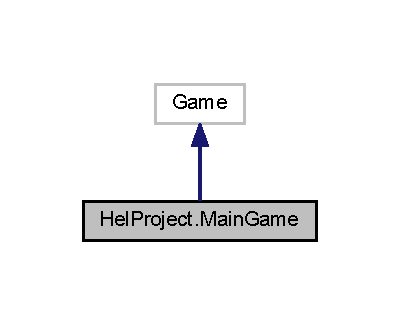
\includegraphics[width=192pt]{class_hel_project_1_1_main_game__inherit__graph}
\end{center}
\end{figure}


Collaboration diagram for Hel\+Project.\+Main\+Game\+:\nopagebreak
\begin{figure}[H]
\begin{center}
\leavevmode
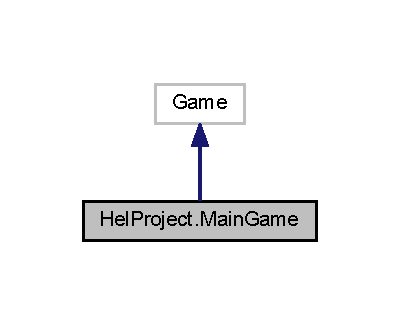
\includegraphics[width=192pt]{class_hel_project_1_1_main_game__coll__graph}
\end{center}
\end{figure}
\subsection*{Protected Member Functions}
\begin{DoxyCompactItemize}
\item 
override void \hyperlink{class_hel_project_1_1_main_game_ada9330a851988897b9e0832853e34950}{Initialize} ()
\begin{DoxyCompactList}\small\item\em Allows the game to perform any initialization it needs to before starting to run. This is where it can query for any required services and load any non-\/graphic related content. Calling base. Initialize will enumerate through any components and initialize them as well. \end{DoxyCompactList}\item 
override void \hyperlink{class_hel_project_1_1_main_game_a2bc21b348062dd85d99efd3822af3e6a}{Load\+Content} ()
\begin{DoxyCompactList}\small\item\em Load\+Content will be called once per game and is the place to load all of your content. \end{DoxyCompactList}\item 
override void \hyperlink{class_hel_project_1_1_main_game_a39242071cf9919f8a8641be9e8396634}{Unload\+Content} ()
\begin{DoxyCompactList}\small\item\em Unload\+Content will be called once per game and is the place to unload all content. \end{DoxyCompactList}\item 
override void \hyperlink{class_hel_project_1_1_main_game_a9ac722d731f12668bb191921101dbba5}{Update} (Game\+Time game\+Time)
\begin{DoxyCompactList}\small\item\em Allows the game to run logic such as updating the world, checking for collisions, gathering input, and playing audio. \end{DoxyCompactList}\item 
override void \hyperlink{class_hel_project_1_1_main_game_a8c0f9655e1d757dad7c35cf5a4529035}{Draw} (Game\+Time game\+Time)
\begin{DoxyCompactList}\small\item\em This is called when the game should draw itself. \end{DoxyCompactList}\end{DoxyCompactItemize}
\subsection*{Properties}
\begin{DoxyCompactItemize}
\item 
static \hyperlink{class_hel_project_1_1_main_game}{Main\+Game} \hyperlink{class_hel_project_1_1_main_game_a19713891cdb3cbae8da8a0bf69ed54f4}{Instance}\hspace{0.3cm}{\ttfamily  \mbox{[}get\mbox{]}}
\begin{DoxyCompactList}\small\item\em Instance of the Main Game \end{DoxyCompactList}\end{DoxyCompactItemize}


\subsection{Detailed Description}
This is the main type for your game 



\subsection{Member Function Documentation}
\hypertarget{class_hel_project_1_1_main_game_a8c0f9655e1d757dad7c35cf5a4529035}{}\index{Hel\+Project\+::\+Main\+Game@{Hel\+Project\+::\+Main\+Game}!Draw@{Draw}}
\index{Draw@{Draw}!Hel\+Project\+::\+Main\+Game@{Hel\+Project\+::\+Main\+Game}}
\subsubsection[{Draw}]{\setlength{\rightskip}{0pt plus 5cm}override void Hel\+Project.\+Main\+Game.\+Draw (
\begin{DoxyParamCaption}
\item[{Game\+Time}]{game\+Time}
\end{DoxyParamCaption}
)\hspace{0.3cm}{\ttfamily [protected]}}\label{class_hel_project_1_1_main_game_a8c0f9655e1d757dad7c35cf5a4529035}


This is called when the game should draw itself. 


\begin{DoxyParams}{Parameters}
{\em game\+Time} & Provides a snapshot of timing values.\\
\hline
\end{DoxyParams}
\hypertarget{class_hel_project_1_1_main_game_ada9330a851988897b9e0832853e34950}{}\index{Hel\+Project\+::\+Main\+Game@{Hel\+Project\+::\+Main\+Game}!Initialize@{Initialize}}
\index{Initialize@{Initialize}!Hel\+Project\+::\+Main\+Game@{Hel\+Project\+::\+Main\+Game}}
\subsubsection[{Initialize}]{\setlength{\rightskip}{0pt plus 5cm}override void Hel\+Project.\+Main\+Game.\+Initialize (
\begin{DoxyParamCaption}
{}
\end{DoxyParamCaption}
)\hspace{0.3cm}{\ttfamily [protected]}}\label{class_hel_project_1_1_main_game_ada9330a851988897b9e0832853e34950}


Allows the game to perform any initialization it needs to before starting to run. This is where it can query for any required services and load any non-\/graphic related content. Calling base. Initialize will enumerate through any components and initialize them as well. 

\hypertarget{class_hel_project_1_1_main_game_a2bc21b348062dd85d99efd3822af3e6a}{}\index{Hel\+Project\+::\+Main\+Game@{Hel\+Project\+::\+Main\+Game}!Load\+Content@{Load\+Content}}
\index{Load\+Content@{Load\+Content}!Hel\+Project\+::\+Main\+Game@{Hel\+Project\+::\+Main\+Game}}
\subsubsection[{Load\+Content}]{\setlength{\rightskip}{0pt plus 5cm}override void Hel\+Project.\+Main\+Game.\+Load\+Content (
\begin{DoxyParamCaption}
{}
\end{DoxyParamCaption}
)\hspace{0.3cm}{\ttfamily [protected]}}\label{class_hel_project_1_1_main_game_a2bc21b348062dd85d99efd3822af3e6a}


Load\+Content will be called once per game and is the place to load all of your content. 

\hypertarget{class_hel_project_1_1_main_game_a39242071cf9919f8a8641be9e8396634}{}\index{Hel\+Project\+::\+Main\+Game@{Hel\+Project\+::\+Main\+Game}!Unload\+Content@{Unload\+Content}}
\index{Unload\+Content@{Unload\+Content}!Hel\+Project\+::\+Main\+Game@{Hel\+Project\+::\+Main\+Game}}
\subsubsection[{Unload\+Content}]{\setlength{\rightskip}{0pt plus 5cm}override void Hel\+Project.\+Main\+Game.\+Unload\+Content (
\begin{DoxyParamCaption}
{}
\end{DoxyParamCaption}
)\hspace{0.3cm}{\ttfamily [protected]}}\label{class_hel_project_1_1_main_game_a39242071cf9919f8a8641be9e8396634}


Unload\+Content will be called once per game and is the place to unload all content. 

\hypertarget{class_hel_project_1_1_main_game_a9ac722d731f12668bb191921101dbba5}{}\index{Hel\+Project\+::\+Main\+Game@{Hel\+Project\+::\+Main\+Game}!Update@{Update}}
\index{Update@{Update}!Hel\+Project\+::\+Main\+Game@{Hel\+Project\+::\+Main\+Game}}
\subsubsection[{Update}]{\setlength{\rightskip}{0pt plus 5cm}override void Hel\+Project.\+Main\+Game.\+Update (
\begin{DoxyParamCaption}
\item[{Game\+Time}]{game\+Time}
\end{DoxyParamCaption}
)\hspace{0.3cm}{\ttfamily [protected]}}\label{class_hel_project_1_1_main_game_a9ac722d731f12668bb191921101dbba5}


Allows the game to run logic such as updating the world, checking for collisions, gathering input, and playing audio. 


\begin{DoxyParams}{Parameters}
{\em game\+Time} & Provides a snapshot of timing values.\\
\hline
\end{DoxyParams}


\subsection{Property Documentation}
\hypertarget{class_hel_project_1_1_main_game_a19713891cdb3cbae8da8a0bf69ed54f4}{}\index{Hel\+Project\+::\+Main\+Game@{Hel\+Project\+::\+Main\+Game}!Instance@{Instance}}
\index{Instance@{Instance}!Hel\+Project\+::\+Main\+Game@{Hel\+Project\+::\+Main\+Game}}
\subsubsection[{Instance}]{\setlength{\rightskip}{0pt plus 5cm}{\bf Main\+Game} Hel\+Project.\+Main\+Game.\+Instance\hspace{0.3cm}{\ttfamily [static]}, {\ttfamily [get]}}\label{class_hel_project_1_1_main_game_a19713891cdb3cbae8da8a0bf69ed54f4}


Instance of the Main Game 



The documentation for this class was generated from the following file\+:\begin{DoxyCompactItemize}
\item 
src/\+Hel\+Project/Main\+Game.\+cs\end{DoxyCompactItemize}

\hypertarget{class_hel_project_1_1_u_i_1_1_menu_1_1_menu_item}{}\section{Hel\+Project.\+U\+I.\+Menu.\+Menu\+Item Class Reference}
\label{class_hel_project_1_1_u_i_1_1_menu_1_1_menu_item}\index{Hel\+Project.\+U\+I.\+Menu.\+Menu\+Item@{Hel\+Project.\+U\+I.\+Menu.\+Menu\+Item}}
\subsection*{Public Types}
\begin{DoxyCompactItemize}
\item 
enum \hyperlink{class_hel_project_1_1_u_i_1_1_menu_1_1_menu_item_aeb422f96ad792622197d81bea826c282}{Link\+Types} \{ {\bfseries M\+E\+N\+U} = 0, 
{\bfseries G\+A\+M\+E} = 1
 \}
\begin{DoxyCompactList}\small\item\em Types of links in the game \end{DoxyCompactList}\end{DoxyCompactItemize}
\subsection*{Public Member Functions}
\begin{DoxyCompactItemize}
\item 
\hyperlink{class_hel_project_1_1_u_i_1_1_menu_1_1_menu_item_abe9a2c0d8a59bfecf5745e21f8dc0642}{Menu\+Item} ()
\begin{DoxyCompactList}\small\item\em Creates a menu item \end{DoxyCompactList}\item 
\hyperlink{class_hel_project_1_1_u_i_1_1_menu_1_1_menu_item_a8baaafaabc305d97e08fac53df14c889}{Menu\+Item} (\hyperlink{class_hel_project_1_1_u_i_1_1_menu_1_1_menu_item_aeb422f96ad792622197d81bea826c282}{Link\+Types} link\+Type, \hyperlink{class_hel_project_1_1_u_i_1_1_image}{Image} img)
\begin{DoxyCompactList}\small\item\em Creates a menu item \end{DoxyCompactList}\end{DoxyCompactItemize}
\subsection*{Properties}
\begin{DoxyCompactItemize}
\item 
\hypertarget{class_hel_project_1_1_u_i_1_1_menu_1_1_menu_item_aa54732e7477c4e4da85bb7b0d7c607db}{}int {\bfseries Id}\hspace{0.3cm}{\ttfamily  \mbox{[}get, set\mbox{]}}\label{class_hel_project_1_1_u_i_1_1_menu_1_1_menu_item_aa54732e7477c4e4da85bb7b0d7c607db}

\item 
\hyperlink{class_hel_project_1_1_u_i_1_1_image}{Image} \hyperlink{class_hel_project_1_1_u_i_1_1_menu_1_1_menu_item_aa233e38588bdc0878b378d84faf08d01}{Item\+Image}\hspace{0.3cm}{\ttfamily  \mbox{[}get, set\mbox{]}}
\begin{DoxyCompactList}\small\item\em \hyperlink{class_hel_project_1_1_u_i_1_1_image}{Image} of the item \end{DoxyCompactList}\item 
\hyperlink{class_hel_project_1_1_u_i_1_1_menu_1_1_menu_item_aeb422f96ad792622197d81bea826c282}{Link\+Types} \hyperlink{class_hel_project_1_1_u_i_1_1_menu_1_1_menu_item_a4973403225833802c1e4409b5eaf2be3}{Link\+Type}\hspace{0.3cm}{\ttfamily  \mbox{[}get, set\mbox{]}}
\begin{DoxyCompactList}\small\item\em Type of the link of the item \end{DoxyCompactList}\end{DoxyCompactItemize}


\subsection{Member Enumeration Documentation}
\hypertarget{class_hel_project_1_1_u_i_1_1_menu_1_1_menu_item_aeb422f96ad792622197d81bea826c282}{}\index{Hel\+Project\+::\+U\+I\+::\+Menu\+::\+Menu\+Item@{Hel\+Project\+::\+U\+I\+::\+Menu\+::\+Menu\+Item}!Link\+Types@{Link\+Types}}
\index{Link\+Types@{Link\+Types}!Hel\+Project\+::\+U\+I\+::\+Menu\+::\+Menu\+Item@{Hel\+Project\+::\+U\+I\+::\+Menu\+::\+Menu\+Item}}
\subsubsection[{Link\+Types}]{\setlength{\rightskip}{0pt plus 5cm}enum {\bf Hel\+Project.\+U\+I.\+Menu.\+Menu\+Item.\+Link\+Types}}\label{class_hel_project_1_1_u_i_1_1_menu_1_1_menu_item_aeb422f96ad792622197d81bea826c282}


Types of links in the game 



\subsection{Constructor \& Destructor Documentation}
\hypertarget{class_hel_project_1_1_u_i_1_1_menu_1_1_menu_item_abe9a2c0d8a59bfecf5745e21f8dc0642}{}\index{Hel\+Project\+::\+U\+I\+::\+Menu\+::\+Menu\+Item@{Hel\+Project\+::\+U\+I\+::\+Menu\+::\+Menu\+Item}!Menu\+Item@{Menu\+Item}}
\index{Menu\+Item@{Menu\+Item}!Hel\+Project\+::\+U\+I\+::\+Menu\+::\+Menu\+Item@{Hel\+Project\+::\+U\+I\+::\+Menu\+::\+Menu\+Item}}
\subsubsection[{Menu\+Item}]{\setlength{\rightskip}{0pt plus 5cm}Hel\+Project.\+U\+I.\+Menu.\+Menu\+Item.\+Menu\+Item (
\begin{DoxyParamCaption}
{}
\end{DoxyParamCaption}
)}\label{class_hel_project_1_1_u_i_1_1_menu_1_1_menu_item_abe9a2c0d8a59bfecf5745e21f8dc0642}


Creates a menu item 

\hypertarget{class_hel_project_1_1_u_i_1_1_menu_1_1_menu_item_a8baaafaabc305d97e08fac53df14c889}{}\index{Hel\+Project\+::\+U\+I\+::\+Menu\+::\+Menu\+Item@{Hel\+Project\+::\+U\+I\+::\+Menu\+::\+Menu\+Item}!Menu\+Item@{Menu\+Item}}
\index{Menu\+Item@{Menu\+Item}!Hel\+Project\+::\+U\+I\+::\+Menu\+::\+Menu\+Item@{Hel\+Project\+::\+U\+I\+::\+Menu\+::\+Menu\+Item}}
\subsubsection[{Menu\+Item}]{\setlength{\rightskip}{0pt plus 5cm}Hel\+Project.\+U\+I.\+Menu.\+Menu\+Item.\+Menu\+Item (
\begin{DoxyParamCaption}
\item[{{\bf Link\+Types}}]{link\+Type, }
\item[{{\bf Image}}]{img}
\end{DoxyParamCaption}
)}\label{class_hel_project_1_1_u_i_1_1_menu_1_1_menu_item_a8baaafaabc305d97e08fac53df14c889}


Creates a menu item 


\begin{DoxyParams}{Parameters}
{\em link\+Type} & Type of the link of the item\\
\hline
{\em img} & \hyperlink{class_hel_project_1_1_u_i_1_1_image}{Image} of the item\\
\hline
\end{DoxyParams}


\subsection{Property Documentation}
\hypertarget{class_hel_project_1_1_u_i_1_1_menu_1_1_menu_item_aa233e38588bdc0878b378d84faf08d01}{}\index{Hel\+Project\+::\+U\+I\+::\+Menu\+::\+Menu\+Item@{Hel\+Project\+::\+U\+I\+::\+Menu\+::\+Menu\+Item}!Item\+Image@{Item\+Image}}
\index{Item\+Image@{Item\+Image}!Hel\+Project\+::\+U\+I\+::\+Menu\+::\+Menu\+Item@{Hel\+Project\+::\+U\+I\+::\+Menu\+::\+Menu\+Item}}
\subsubsection[{Item\+Image}]{\setlength{\rightskip}{0pt plus 5cm}{\bf Image} Hel\+Project.\+U\+I.\+Menu.\+Menu\+Item.\+Item\+Image\hspace{0.3cm}{\ttfamily [get]}, {\ttfamily [set]}}\label{class_hel_project_1_1_u_i_1_1_menu_1_1_menu_item_aa233e38588bdc0878b378d84faf08d01}


\hyperlink{class_hel_project_1_1_u_i_1_1_image}{Image} of the item 

\hypertarget{class_hel_project_1_1_u_i_1_1_menu_1_1_menu_item_a4973403225833802c1e4409b5eaf2be3}{}\index{Hel\+Project\+::\+U\+I\+::\+Menu\+::\+Menu\+Item@{Hel\+Project\+::\+U\+I\+::\+Menu\+::\+Menu\+Item}!Link\+Type@{Link\+Type}}
\index{Link\+Type@{Link\+Type}!Hel\+Project\+::\+U\+I\+::\+Menu\+::\+Menu\+Item@{Hel\+Project\+::\+U\+I\+::\+Menu\+::\+Menu\+Item}}
\subsubsection[{Link\+Type}]{\setlength{\rightskip}{0pt plus 5cm}{\bf Link\+Types} Hel\+Project.\+U\+I.\+Menu.\+Menu\+Item.\+Link\+Type\hspace{0.3cm}{\ttfamily [get]}, {\ttfamily [set]}}\label{class_hel_project_1_1_u_i_1_1_menu_1_1_menu_item_a4973403225833802c1e4409b5eaf2be3}


Type of the link of the item 



The documentation for this class was generated from the following file\+:\begin{DoxyCompactItemize}
\item 
src/\+Hel\+Project/\+U\+I/\+Menu/Menu\+Item.\+cs\end{DoxyCompactItemize}

\hypertarget{class_hel_project_1_1_u_i_1_1_menu_1_1_menu_manager}{}\section{Hel\+Project.\+U\+I.\+Menu.\+Menu\+Manager Class Reference}
\label{class_hel_project_1_1_u_i_1_1_menu_1_1_menu_manager}\index{Hel\+Project.\+U\+I.\+Menu.\+Menu\+Manager@{Hel\+Project.\+U\+I.\+Menu.\+Menu\+Manager}}


The documentation for this class was generated from the following file\+:\begin{DoxyCompactItemize}
\item 
src/\+Hel\+Project/\+U\+I/\+Menu/Menu\+Manager.\+cs\end{DoxyCompactItemize}

\hypertarget{class_hel_project_1_1_u_i_1_1_menu_1_1_menu_screen}{}\section{Hel\+Project.\+U\+I.\+Menu.\+Menu\+Screen Class Reference}
\label{class_hel_project_1_1_u_i_1_1_menu_1_1_menu_screen}\index{Hel\+Project.\+U\+I.\+Menu.\+Menu\+Screen@{Hel\+Project.\+U\+I.\+Menu.\+Menu\+Screen}}


Title screen of the game  




Inheritance diagram for Hel\+Project.\+U\+I.\+Menu.\+Menu\+Screen\+:\nopagebreak
\begin{figure}[H]
\begin{center}
\leavevmode
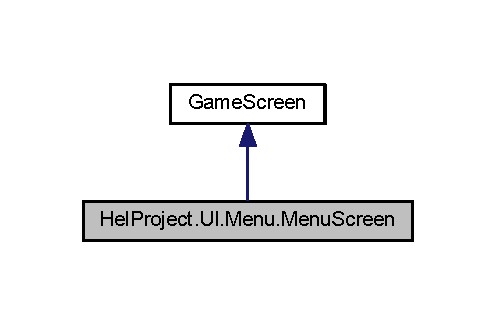
\includegraphics[width=238pt]{class_hel_project_1_1_u_i_1_1_menu_1_1_menu_screen__inherit__graph}
\end{center}
\end{figure}


Collaboration diagram for Hel\+Project.\+U\+I.\+Menu.\+Menu\+Screen\+:\nopagebreak
\begin{figure}[H]
\begin{center}
\leavevmode
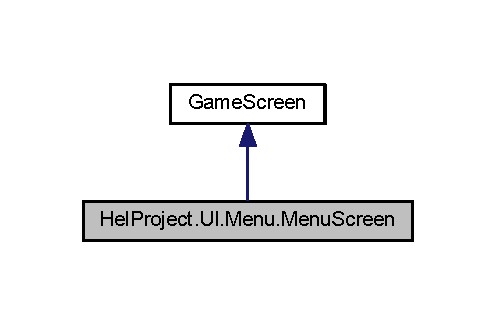
\includegraphics[width=238pt]{class_hel_project_1_1_u_i_1_1_menu_1_1_menu_screen__coll__graph}
\end{center}
\end{figure}
\subsection*{Public Member Functions}
\begin{DoxyCompactItemize}
\item 
\hyperlink{class_hel_project_1_1_u_i_1_1_menu_1_1_menu_screen_af65f39a4c1755b8f24f63b264863ae5a}{Menu\+Screen} ()
\begin{DoxyCompactList}\small\item\em Creates an empty menu \end{DoxyCompactList}\item 
\hyperlink{class_hel_project_1_1_u_i_1_1_menu_1_1_menu_screen_a7c3ca1d57ddee8a977f5172df0070de1}{Menu\+Screen} (Point menu\+Position, List$<$ \hyperlink{class_hel_project_1_1_u_i_1_1_menu_1_1_menu_item}{Menu\+Item} $>$ menu\+Items)
\begin{DoxyCompactList}\small\item\em Creates a menu \end{DoxyCompactList}\item 
\hypertarget{class_hel_project_1_1_u_i_1_1_menu_1_1_menu_screen_af6bc8ddb3fb05ee92f857d95f914f56b}{}{\bfseries Menu\+Screen} (Point menu\+Position, List$<$ \hyperlink{class_hel_project_1_1_u_i_1_1_menu_1_1_menu_item}{Menu\+Item} $>$ menu\+Items, int highlight\+Index)\label{class_hel_project_1_1_u_i_1_1_menu_1_1_menu_screen_af6bc8ddb3fb05ee92f857d95f914f56b}

\item 
override void \hyperlink{class_hel_project_1_1_u_i_1_1_menu_1_1_menu_screen_a6a739ee514c5c05b13a91c5f520a3352}{Load\+Content} ()
\begin{DoxyCompactList}\small\item\em Loads the content of the screen \end{DoxyCompactList}\item 
override void \hyperlink{class_hel_project_1_1_u_i_1_1_menu_1_1_menu_screen_ace5a0a823194e4b39c38e146959e00e1}{Unload\+Content} ()
\begin{DoxyCompactList}\small\item\em Unloads the content of the screen \end{DoxyCompactList}\item 
override void \hyperlink{class_hel_project_1_1_u_i_1_1_menu_1_1_menu_screen_af7295758606c3cb7124983c86a51ecae}{Update} (Game\+Time game\+Time)
\begin{DoxyCompactList}\small\item\em Updates the content of the screen \end{DoxyCompactList}\item 
override void \hyperlink{class_hel_project_1_1_u_i_1_1_menu_1_1_menu_screen_a6a7f006379781977088ac588430c8822}{Draw} (Sprite\+Batch sprite\+Batch)
\begin{DoxyCompactList}\small\item\em Draws the content of the screen \end{DoxyCompactList}\end{DoxyCompactItemize}
\subsection*{Properties}
\begin{DoxyCompactItemize}
\item 
\hyperlink{class_hel_project_1_1_u_i_1_1_image}{Image} \hyperlink{class_hel_project_1_1_u_i_1_1_menu_1_1_menu_screen_a3f4d85faa700315baaa4a5f40bf3576e}{Background\+Image}\hspace{0.3cm}{\ttfamily  \mbox{[}get, set\mbox{]}}
\begin{DoxyCompactList}\small\item\em Background image of the screen \end{DoxyCompactList}\item 
int \hyperlink{class_hel_project_1_1_u_i_1_1_menu_1_1_menu_screen_ad673eedc194957e3e8ecd157bf954f9c}{Highlight\+Index}\hspace{0.3cm}{\ttfamily  \mbox{[}get, set\mbox{]}}
\begin{DoxyCompactList}\small\item\em Index of the highlighted item of the menu \end{DoxyCompactList}\item 
Point \hyperlink{class_hel_project_1_1_u_i_1_1_menu_1_1_menu_screen_a0bd573fd87cbe653e0c8b50fe309de3a}{Menu\+Position}\hspace{0.3cm}{\ttfamily  \mbox{[}get, set\mbox{]}}
\begin{DoxyCompactList}\small\item\em Position of the menu \end{DoxyCompactList}\item 
List$<$ \hyperlink{class_hel_project_1_1_u_i_1_1_menu_1_1_menu_item}{Menu\+Item} $>$ \hyperlink{class_hel_project_1_1_u_i_1_1_menu_1_1_menu_screen_a5c4e68d9b5187dde747e872b719d2886}{Items}\hspace{0.3cm}{\ttfamily  \mbox{[}get, set\mbox{]}}
\begin{DoxyCompactList}\small\item\em Items of the menu \end{DoxyCompactList}\end{DoxyCompactItemize}


\subsection{Detailed Description}
Title screen of the game 



\subsection{Constructor \& Destructor Documentation}
\hypertarget{class_hel_project_1_1_u_i_1_1_menu_1_1_menu_screen_af65f39a4c1755b8f24f63b264863ae5a}{}\index{Hel\+Project\+::\+U\+I\+::\+Menu\+::\+Menu\+Screen@{Hel\+Project\+::\+U\+I\+::\+Menu\+::\+Menu\+Screen}!Menu\+Screen@{Menu\+Screen}}
\index{Menu\+Screen@{Menu\+Screen}!Hel\+Project\+::\+U\+I\+::\+Menu\+::\+Menu\+Screen@{Hel\+Project\+::\+U\+I\+::\+Menu\+::\+Menu\+Screen}}
\subsubsection[{Menu\+Screen}]{\setlength{\rightskip}{0pt plus 5cm}Hel\+Project.\+U\+I.\+Menu.\+Menu\+Screen.\+Menu\+Screen (
\begin{DoxyParamCaption}
{}
\end{DoxyParamCaption}
)}\label{class_hel_project_1_1_u_i_1_1_menu_1_1_menu_screen_af65f39a4c1755b8f24f63b264863ae5a}


Creates an empty menu 

\hypertarget{class_hel_project_1_1_u_i_1_1_menu_1_1_menu_screen_a7c3ca1d57ddee8a977f5172df0070de1}{}\index{Hel\+Project\+::\+U\+I\+::\+Menu\+::\+Menu\+Screen@{Hel\+Project\+::\+U\+I\+::\+Menu\+::\+Menu\+Screen}!Menu\+Screen@{Menu\+Screen}}
\index{Menu\+Screen@{Menu\+Screen}!Hel\+Project\+::\+U\+I\+::\+Menu\+::\+Menu\+Screen@{Hel\+Project\+::\+U\+I\+::\+Menu\+::\+Menu\+Screen}}
\subsubsection[{Menu\+Screen}]{\setlength{\rightskip}{0pt plus 5cm}Hel\+Project.\+U\+I.\+Menu.\+Menu\+Screen.\+Menu\+Screen (
\begin{DoxyParamCaption}
\item[{Point}]{menu\+Position, }
\item[{List$<$ {\bf Menu\+Item} $>$}]{menu\+Items}
\end{DoxyParamCaption}
)}\label{class_hel_project_1_1_u_i_1_1_menu_1_1_menu_screen_a7c3ca1d57ddee8a977f5172df0070de1}


Creates a menu 


\begin{DoxyParams}{Parameters}
{\em menu\+Position} & Position of the menu\\
\hline
{\em menu\+Items} & Items of the menu\\
\hline
\end{DoxyParams}


\subsection{Member Function Documentation}
\hypertarget{class_hel_project_1_1_u_i_1_1_menu_1_1_menu_screen_a6a7f006379781977088ac588430c8822}{}\index{Hel\+Project\+::\+U\+I\+::\+Menu\+::\+Menu\+Screen@{Hel\+Project\+::\+U\+I\+::\+Menu\+::\+Menu\+Screen}!Draw@{Draw}}
\index{Draw@{Draw}!Hel\+Project\+::\+U\+I\+::\+Menu\+::\+Menu\+Screen@{Hel\+Project\+::\+U\+I\+::\+Menu\+::\+Menu\+Screen}}
\subsubsection[{Draw}]{\setlength{\rightskip}{0pt plus 5cm}override void Hel\+Project.\+U\+I.\+Menu.\+Menu\+Screen.\+Draw (
\begin{DoxyParamCaption}
\item[{Sprite\+Batch}]{sprite\+Batch}
\end{DoxyParamCaption}
)\hspace{0.3cm}{\ttfamily [virtual]}}\label{class_hel_project_1_1_u_i_1_1_menu_1_1_menu_screen_a6a7f006379781977088ac588430c8822}


Draws the content of the screen 


\begin{DoxyParams}{Parameters}
{\em sprite\+Batch} & \\
\hline
\end{DoxyParams}


Reimplemented from \hyperlink{class_hel_project_1_1_u_i_1_1_game_screen_ace6f51c0a6c5206a5c58cefd0eba2797}{Hel\+Project.\+U\+I.\+Game\+Screen}.

\hypertarget{class_hel_project_1_1_u_i_1_1_menu_1_1_menu_screen_a6a739ee514c5c05b13a91c5f520a3352}{}\index{Hel\+Project\+::\+U\+I\+::\+Menu\+::\+Menu\+Screen@{Hel\+Project\+::\+U\+I\+::\+Menu\+::\+Menu\+Screen}!Load\+Content@{Load\+Content}}
\index{Load\+Content@{Load\+Content}!Hel\+Project\+::\+U\+I\+::\+Menu\+::\+Menu\+Screen@{Hel\+Project\+::\+U\+I\+::\+Menu\+::\+Menu\+Screen}}
\subsubsection[{Load\+Content}]{\setlength{\rightskip}{0pt plus 5cm}override void Hel\+Project.\+U\+I.\+Menu.\+Menu\+Screen.\+Load\+Content (
\begin{DoxyParamCaption}
{}
\end{DoxyParamCaption}
)\hspace{0.3cm}{\ttfamily [virtual]}}\label{class_hel_project_1_1_u_i_1_1_menu_1_1_menu_screen_a6a739ee514c5c05b13a91c5f520a3352}


Loads the content of the screen 



Reimplemented from \hyperlink{class_hel_project_1_1_u_i_1_1_game_screen_aa4e15890ede3b8da390ffe0cecff3703}{Hel\+Project.\+U\+I.\+Game\+Screen}.

\hypertarget{class_hel_project_1_1_u_i_1_1_menu_1_1_menu_screen_ace5a0a823194e4b39c38e146959e00e1}{}\index{Hel\+Project\+::\+U\+I\+::\+Menu\+::\+Menu\+Screen@{Hel\+Project\+::\+U\+I\+::\+Menu\+::\+Menu\+Screen}!Unload\+Content@{Unload\+Content}}
\index{Unload\+Content@{Unload\+Content}!Hel\+Project\+::\+U\+I\+::\+Menu\+::\+Menu\+Screen@{Hel\+Project\+::\+U\+I\+::\+Menu\+::\+Menu\+Screen}}
\subsubsection[{Unload\+Content}]{\setlength{\rightskip}{0pt plus 5cm}override void Hel\+Project.\+U\+I.\+Menu.\+Menu\+Screen.\+Unload\+Content (
\begin{DoxyParamCaption}
{}
\end{DoxyParamCaption}
)\hspace{0.3cm}{\ttfamily [virtual]}}\label{class_hel_project_1_1_u_i_1_1_menu_1_1_menu_screen_ace5a0a823194e4b39c38e146959e00e1}


Unloads the content of the screen 



Reimplemented from \hyperlink{class_hel_project_1_1_u_i_1_1_game_screen_a97560de3aeb8b283fca89c1682ec778f}{Hel\+Project.\+U\+I.\+Game\+Screen}.

\hypertarget{class_hel_project_1_1_u_i_1_1_menu_1_1_menu_screen_af7295758606c3cb7124983c86a51ecae}{}\index{Hel\+Project\+::\+U\+I\+::\+Menu\+::\+Menu\+Screen@{Hel\+Project\+::\+U\+I\+::\+Menu\+::\+Menu\+Screen}!Update@{Update}}
\index{Update@{Update}!Hel\+Project\+::\+U\+I\+::\+Menu\+::\+Menu\+Screen@{Hel\+Project\+::\+U\+I\+::\+Menu\+::\+Menu\+Screen}}
\subsubsection[{Update}]{\setlength{\rightskip}{0pt plus 5cm}override void Hel\+Project.\+U\+I.\+Menu.\+Menu\+Screen.\+Update (
\begin{DoxyParamCaption}
\item[{Game\+Time}]{game\+Time}
\end{DoxyParamCaption}
)\hspace{0.3cm}{\ttfamily [virtual]}}\label{class_hel_project_1_1_u_i_1_1_menu_1_1_menu_screen_af7295758606c3cb7124983c86a51ecae}


Updates the content of the screen 


\begin{DoxyParams}{Parameters}
{\em game\+Time} & \\
\hline
\end{DoxyParams}


Reimplemented from \hyperlink{class_hel_project_1_1_u_i_1_1_game_screen_a4aefe31814b0081be3ba4f1243b8cee6}{Hel\+Project.\+U\+I.\+Game\+Screen}.



\subsection{Property Documentation}
\hypertarget{class_hel_project_1_1_u_i_1_1_menu_1_1_menu_screen_a3f4d85faa700315baaa4a5f40bf3576e}{}\index{Hel\+Project\+::\+U\+I\+::\+Menu\+::\+Menu\+Screen@{Hel\+Project\+::\+U\+I\+::\+Menu\+::\+Menu\+Screen}!Background\+Image@{Background\+Image}}
\index{Background\+Image@{Background\+Image}!Hel\+Project\+::\+U\+I\+::\+Menu\+::\+Menu\+Screen@{Hel\+Project\+::\+U\+I\+::\+Menu\+::\+Menu\+Screen}}
\subsubsection[{Background\+Image}]{\setlength{\rightskip}{0pt plus 5cm}{\bf Image} Hel\+Project.\+U\+I.\+Menu.\+Menu\+Screen.\+Background\+Image\hspace{0.3cm}{\ttfamily [get]}, {\ttfamily [set]}}\label{class_hel_project_1_1_u_i_1_1_menu_1_1_menu_screen_a3f4d85faa700315baaa4a5f40bf3576e}


Background image of the screen 

\hypertarget{class_hel_project_1_1_u_i_1_1_menu_1_1_menu_screen_ad673eedc194957e3e8ecd157bf954f9c}{}\index{Hel\+Project\+::\+U\+I\+::\+Menu\+::\+Menu\+Screen@{Hel\+Project\+::\+U\+I\+::\+Menu\+::\+Menu\+Screen}!Highlight\+Index@{Highlight\+Index}}
\index{Highlight\+Index@{Highlight\+Index}!Hel\+Project\+::\+U\+I\+::\+Menu\+::\+Menu\+Screen@{Hel\+Project\+::\+U\+I\+::\+Menu\+::\+Menu\+Screen}}
\subsubsection[{Highlight\+Index}]{\setlength{\rightskip}{0pt plus 5cm}int Hel\+Project.\+U\+I.\+Menu.\+Menu\+Screen.\+Highlight\+Index\hspace{0.3cm}{\ttfamily [get]}, {\ttfamily [set]}}\label{class_hel_project_1_1_u_i_1_1_menu_1_1_menu_screen_ad673eedc194957e3e8ecd157bf954f9c}


Index of the highlighted item of the menu 

\hypertarget{class_hel_project_1_1_u_i_1_1_menu_1_1_menu_screen_a5c4e68d9b5187dde747e872b719d2886}{}\index{Hel\+Project\+::\+U\+I\+::\+Menu\+::\+Menu\+Screen@{Hel\+Project\+::\+U\+I\+::\+Menu\+::\+Menu\+Screen}!Items@{Items}}
\index{Items@{Items}!Hel\+Project\+::\+U\+I\+::\+Menu\+::\+Menu\+Screen@{Hel\+Project\+::\+U\+I\+::\+Menu\+::\+Menu\+Screen}}
\subsubsection[{Items}]{\setlength{\rightskip}{0pt plus 5cm}List$<${\bf Menu\+Item}$>$ Hel\+Project.\+U\+I.\+Menu.\+Menu\+Screen.\+Items\hspace{0.3cm}{\ttfamily [get]}, {\ttfamily [set]}}\label{class_hel_project_1_1_u_i_1_1_menu_1_1_menu_screen_a5c4e68d9b5187dde747e872b719d2886}


Items of the menu 

\hypertarget{class_hel_project_1_1_u_i_1_1_menu_1_1_menu_screen_a0bd573fd87cbe653e0c8b50fe309de3a}{}\index{Hel\+Project\+::\+U\+I\+::\+Menu\+::\+Menu\+Screen@{Hel\+Project\+::\+U\+I\+::\+Menu\+::\+Menu\+Screen}!Menu\+Position@{Menu\+Position}}
\index{Menu\+Position@{Menu\+Position}!Hel\+Project\+::\+U\+I\+::\+Menu\+::\+Menu\+Screen@{Hel\+Project\+::\+U\+I\+::\+Menu\+::\+Menu\+Screen}}
\subsubsection[{Menu\+Position}]{\setlength{\rightskip}{0pt plus 5cm}Point Hel\+Project.\+U\+I.\+Menu.\+Menu\+Screen.\+Menu\+Position\hspace{0.3cm}{\ttfamily [get]}, {\ttfamily [set]}}\label{class_hel_project_1_1_u_i_1_1_menu_1_1_menu_screen_a0bd573fd87cbe653e0c8b50fe309de3a}


Position of the menu 



The documentation for this class was generated from the following file\+:\begin{DoxyCompactItemize}
\item 
src/\+Hel\+Project/\+U\+I/\+Menu/Menu\+Screen.\+cs\end{DoxyCompactItemize}

\hypertarget{class_hel_project_1_1_u_i_1_1_play_screen}{}\section{Hel\+Project.\+U\+I.\+Play\+Screen Class Reference}
\label{class_hel_project_1_1_u_i_1_1_play_screen}\index{Hel\+Project.\+U\+I.\+Play\+Screen@{Hel\+Project.\+U\+I.\+Play\+Screen}}


Screen for the gameplay  




Inheritance diagram for Hel\+Project.\+U\+I.\+Play\+Screen\+:\nopagebreak
\begin{figure}[H]
\begin{center}
\leavevmode
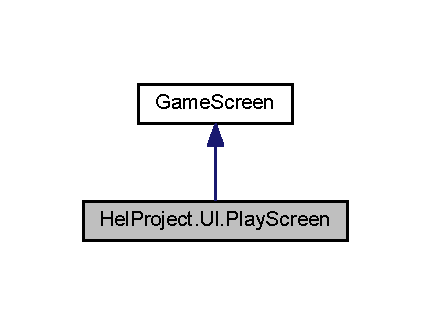
\includegraphics[width=207pt]{class_hel_project_1_1_u_i_1_1_play_screen__inherit__graph}
\end{center}
\end{figure}


Collaboration diagram for Hel\+Project.\+U\+I.\+Play\+Screen\+:\nopagebreak
\begin{figure}[H]
\begin{center}
\leavevmode
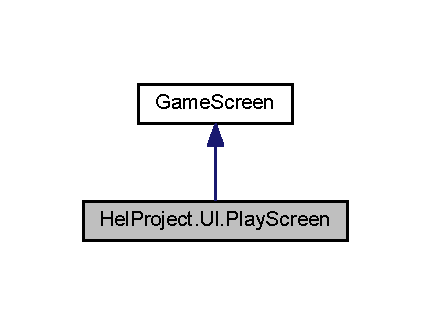
\includegraphics[width=207pt]{class_hel_project_1_1_u_i_1_1_play_screen__coll__graph}
\end{center}
\end{figure}
\subsection*{Public Member Functions}
\begin{DoxyCompactItemize}
\item 
override void \hyperlink{class_hel_project_1_1_u_i_1_1_play_screen_af3639840bdd8de714d262377c417ee20}{Load\+Content} ()
\begin{DoxyCompactList}\small\item\em Loads the content of the window \end{DoxyCompactList}\item 
override void \hyperlink{class_hel_project_1_1_u_i_1_1_play_screen_a90c75361ad40bff449d2a560ef8f4464}{Unload\+Content} ()
\begin{DoxyCompactList}\small\item\em Unloads the content of the window \end{DoxyCompactList}\item 
override void \hyperlink{class_hel_project_1_1_u_i_1_1_play_screen_a012a79b297f9e09a0d21dbe952a653db}{Update} (Game\+Time game\+Time)
\begin{DoxyCompactList}\small\item\em Updates the mechanisms \end{DoxyCompactList}\item 
override void \hyperlink{class_hel_project_1_1_u_i_1_1_play_screen_a0f290e8d07d6632fd53a66efc585e853}{Draw} (Sprite\+Batch sprite\+Batch)
\begin{DoxyCompactList}\small\item\em Draws on the window \end{DoxyCompactList}\item 
void \hyperlink{class_hel_project_1_1_u_i_1_1_play_screen_a0b4785cbfbf29d287b40c003a2b0001d}{Transition\+To\+Map} (\hyperlink{class_hel_project_1_1_game_world_1_1_map_1_1_h_map}{H\+Map} map)
\begin{DoxyCompactList}\small\item\em Transitions to another map \end{DoxyCompactList}\end{DoxyCompactItemize}
\subsection*{Properties}
\begin{DoxyCompactItemize}
\item 
\hyperlink{class_hel_project_1_1_u_i_1_1_selection_aid}{Selection\+Aid} \hyperlink{class_hel_project_1_1_u_i_1_1_play_screen_a06addd08f18e59b70cded27e325a6ed1}{Selection\+Assistant}\hspace{0.3cm}{\ttfamily  \mbox{[}get, set\mbox{]}}
\begin{DoxyCompactList}\small\item\em Selection assistant for the game \end{DoxyCompactList}\item 
\hyperlink{class_hel_project_1_1_game_world_1_1_map_1_1_h_map}{H\+Map} \hyperlink{class_hel_project_1_1_u_i_1_1_play_screen_a8f6f7d590c13e9f21db49c181daabc32}{Map\+Town}\hspace{0.3cm}{\ttfamily  \mbox{[}get, set\mbox{]}}
\begin{DoxyCompactList}\small\item\em Starting point of the game \+: The town \end{DoxyCompactList}\item 
\hyperlink{class_hel_project_1_1_game_world_1_1_map_1_1_h_map}{H\+Map} \hyperlink{class_hel_project_1_1_u_i_1_1_play_screen_a6fa66d24cfdc2801ecfd0e72f1c1669b}{Map\+Difficulty\+Easy}\hspace{0.3cm}{\ttfamily  \mbox{[}get, set\mbox{]}}
\begin{DoxyCompactList}\small\item\em Map of the game with easy difficulty \end{DoxyCompactList}\item 
\hyperlink{class_hel_project_1_1_game_world_1_1_map_1_1_h_map}{H\+Map} \hyperlink{class_hel_project_1_1_u_i_1_1_play_screen_a4dc67a0bb9e4dfc7fabcb35e45529771}{Map\+Difficulty\+Medium}\hspace{0.3cm}{\ttfamily  \mbox{[}get, set\mbox{]}}
\begin{DoxyCompactList}\small\item\em Map of the game with medium difficulty \end{DoxyCompactList}\item 
\hyperlink{class_hel_project_1_1_game_world_1_1_map_1_1_h_map}{H\+Map} \hyperlink{class_hel_project_1_1_u_i_1_1_play_screen_a8dd43c45856c0c6ed338e214e4009d2d}{Map\+Difficulty\+Hard}\hspace{0.3cm}{\ttfamily  \mbox{[}get, set\mbox{]}}
\begin{DoxyCompactList}\small\item\em Map of the game with hard difficulty \end{DoxyCompactList}\item 
\hyperlink{class_hel_project_1_1_game_world_1_1_map_1_1_h_map}{H\+Map} \hyperlink{class_hel_project_1_1_u_i_1_1_play_screen_ad7c470e2c8f452c734ec3dc1fa6e3061}{Current\+Map}\hspace{0.3cm}{\ttfamily  \mbox{[}get, set\mbox{]}}
\begin{DoxyCompactList}\small\item\em Current map where the hero is \end{DoxyCompactList}\item 
\hyperlink{class_hel_project_1_1_game_world_1_1_entities_1_1_h_hero}{H\+Hero} \hyperlink{class_hel_project_1_1_u_i_1_1_play_screen_a404ed230e991ee3a7563c23fc053f383}{Playable\+Character}\hspace{0.3cm}{\ttfamily  \mbox{[}get, set\mbox{]}}
\begin{DoxyCompactList}\small\item\em Playable character \end{DoxyCompactList}\item 
static \hyperlink{class_hel_project_1_1_u_i_1_1_play_screen}{Play\+Screen} \hyperlink{class_hel_project_1_1_u_i_1_1_play_screen_a0611d9168457e37ecfd8a1758dc0f969}{Instance}\hspace{0.3cm}{\ttfamily  \mbox{[}get\mbox{]}}
\begin{DoxyCompactList}\small\item\em Instance of the play screen \end{DoxyCompactList}\item 
\hyperlink{class_hel_project_1_1_u_i_1_1_camera}{Camera} \hyperlink{class_hel_project_1_1_u_i_1_1_play_screen_a1b972d98ea08568609caa80db4d22dd7}{Camera}\hspace{0.3cm}{\ttfamily  \mbox{[}get, set\mbox{]}}
\begin{DoxyCompactList}\small\item\em \hyperlink{class_hel_project_1_1_u_i_1_1_camera}{Camera} of the play screen \end{DoxyCompactList}\end{DoxyCompactItemize}


\subsection{Detailed Description}
Screen for the gameplay 



\subsection{Member Function Documentation}
\hypertarget{class_hel_project_1_1_u_i_1_1_play_screen_a0f290e8d07d6632fd53a66efc585e853}{}\index{Hel\+Project\+::\+U\+I\+::\+Play\+Screen@{Hel\+Project\+::\+U\+I\+::\+Play\+Screen}!Draw@{Draw}}
\index{Draw@{Draw}!Hel\+Project\+::\+U\+I\+::\+Play\+Screen@{Hel\+Project\+::\+U\+I\+::\+Play\+Screen}}
\subsubsection[{Draw}]{\setlength{\rightskip}{0pt plus 5cm}override void Hel\+Project.\+U\+I.\+Play\+Screen.\+Draw (
\begin{DoxyParamCaption}
\item[{Sprite\+Batch}]{sprite\+Batch}
\end{DoxyParamCaption}
)\hspace{0.3cm}{\ttfamily [virtual]}}\label{class_hel_project_1_1_u_i_1_1_play_screen_a0f290e8d07d6632fd53a66efc585e853}


Draws on the window 


\begin{DoxyParams}{Parameters}
{\em sprite\+Batch} & \\
\hline
\end{DoxyParams}


Reimplemented from \hyperlink{class_hel_project_1_1_u_i_1_1_game_screen_ace6f51c0a6c5206a5c58cefd0eba2797}{Hel\+Project.\+U\+I.\+Game\+Screen}.

\hypertarget{class_hel_project_1_1_u_i_1_1_play_screen_af3639840bdd8de714d262377c417ee20}{}\index{Hel\+Project\+::\+U\+I\+::\+Play\+Screen@{Hel\+Project\+::\+U\+I\+::\+Play\+Screen}!Load\+Content@{Load\+Content}}
\index{Load\+Content@{Load\+Content}!Hel\+Project\+::\+U\+I\+::\+Play\+Screen@{Hel\+Project\+::\+U\+I\+::\+Play\+Screen}}
\subsubsection[{Load\+Content}]{\setlength{\rightskip}{0pt plus 5cm}override void Hel\+Project.\+U\+I.\+Play\+Screen.\+Load\+Content (
\begin{DoxyParamCaption}
{}
\end{DoxyParamCaption}
)\hspace{0.3cm}{\ttfamily [virtual]}}\label{class_hel_project_1_1_u_i_1_1_play_screen_af3639840bdd8de714d262377c417ee20}


Loads the content of the window 



Reimplemented from \hyperlink{class_hel_project_1_1_u_i_1_1_game_screen_aa4e15890ede3b8da390ffe0cecff3703}{Hel\+Project.\+U\+I.\+Game\+Screen}.

\hypertarget{class_hel_project_1_1_u_i_1_1_play_screen_a0b4785cbfbf29d287b40c003a2b0001d}{}\index{Hel\+Project\+::\+U\+I\+::\+Play\+Screen@{Hel\+Project\+::\+U\+I\+::\+Play\+Screen}!Transition\+To\+Map@{Transition\+To\+Map}}
\index{Transition\+To\+Map@{Transition\+To\+Map}!Hel\+Project\+::\+U\+I\+::\+Play\+Screen@{Hel\+Project\+::\+U\+I\+::\+Play\+Screen}}
\subsubsection[{Transition\+To\+Map}]{\setlength{\rightskip}{0pt plus 5cm}void Hel\+Project.\+U\+I.\+Play\+Screen.\+Transition\+To\+Map (
\begin{DoxyParamCaption}
\item[{{\bf H\+Map}}]{map}
\end{DoxyParamCaption}
)}\label{class_hel_project_1_1_u_i_1_1_play_screen_a0b4785cbfbf29d287b40c003a2b0001d}


Transitions to another map 


\begin{DoxyParams}{Parameters}
{\em map} & \\
\hline
\end{DoxyParams}
\hypertarget{class_hel_project_1_1_u_i_1_1_play_screen_a90c75361ad40bff449d2a560ef8f4464}{}\index{Hel\+Project\+::\+U\+I\+::\+Play\+Screen@{Hel\+Project\+::\+U\+I\+::\+Play\+Screen}!Unload\+Content@{Unload\+Content}}
\index{Unload\+Content@{Unload\+Content}!Hel\+Project\+::\+U\+I\+::\+Play\+Screen@{Hel\+Project\+::\+U\+I\+::\+Play\+Screen}}
\subsubsection[{Unload\+Content}]{\setlength{\rightskip}{0pt plus 5cm}override void Hel\+Project.\+U\+I.\+Play\+Screen.\+Unload\+Content (
\begin{DoxyParamCaption}
{}
\end{DoxyParamCaption}
)\hspace{0.3cm}{\ttfamily [virtual]}}\label{class_hel_project_1_1_u_i_1_1_play_screen_a90c75361ad40bff449d2a560ef8f4464}


Unloads the content of the window 



Reimplemented from \hyperlink{class_hel_project_1_1_u_i_1_1_game_screen_a97560de3aeb8b283fca89c1682ec778f}{Hel\+Project.\+U\+I.\+Game\+Screen}.

\hypertarget{class_hel_project_1_1_u_i_1_1_play_screen_a012a79b297f9e09a0d21dbe952a653db}{}\index{Hel\+Project\+::\+U\+I\+::\+Play\+Screen@{Hel\+Project\+::\+U\+I\+::\+Play\+Screen}!Update@{Update}}
\index{Update@{Update}!Hel\+Project\+::\+U\+I\+::\+Play\+Screen@{Hel\+Project\+::\+U\+I\+::\+Play\+Screen}}
\subsubsection[{Update}]{\setlength{\rightskip}{0pt plus 5cm}override void Hel\+Project.\+U\+I.\+Play\+Screen.\+Update (
\begin{DoxyParamCaption}
\item[{Game\+Time}]{game\+Time}
\end{DoxyParamCaption}
)\hspace{0.3cm}{\ttfamily [virtual]}}\label{class_hel_project_1_1_u_i_1_1_play_screen_a012a79b297f9e09a0d21dbe952a653db}


Updates the mechanisms 


\begin{DoxyParams}{Parameters}
{\em game\+Time} & \\
\hline
\end{DoxyParams}


Reimplemented from \hyperlink{class_hel_project_1_1_u_i_1_1_game_screen_a4aefe31814b0081be3ba4f1243b8cee6}{Hel\+Project.\+U\+I.\+Game\+Screen}.



\subsection{Property Documentation}
\hypertarget{class_hel_project_1_1_u_i_1_1_play_screen_a1b972d98ea08568609caa80db4d22dd7}{}\index{Hel\+Project\+::\+U\+I\+::\+Play\+Screen@{Hel\+Project\+::\+U\+I\+::\+Play\+Screen}!Camera@{Camera}}
\index{Camera@{Camera}!Hel\+Project\+::\+U\+I\+::\+Play\+Screen@{Hel\+Project\+::\+U\+I\+::\+Play\+Screen}}
\subsubsection[{Camera}]{\setlength{\rightskip}{0pt plus 5cm}{\bf Camera} Hel\+Project.\+U\+I.\+Play\+Screen.\+Camera\hspace{0.3cm}{\ttfamily [get]}, {\ttfamily [set]}}\label{class_hel_project_1_1_u_i_1_1_play_screen_a1b972d98ea08568609caa80db4d22dd7}


\hyperlink{class_hel_project_1_1_u_i_1_1_camera}{Camera} of the play screen 

\hypertarget{class_hel_project_1_1_u_i_1_1_play_screen_ad7c470e2c8f452c734ec3dc1fa6e3061}{}\index{Hel\+Project\+::\+U\+I\+::\+Play\+Screen@{Hel\+Project\+::\+U\+I\+::\+Play\+Screen}!Current\+Map@{Current\+Map}}
\index{Current\+Map@{Current\+Map}!Hel\+Project\+::\+U\+I\+::\+Play\+Screen@{Hel\+Project\+::\+U\+I\+::\+Play\+Screen}}
\subsubsection[{Current\+Map}]{\setlength{\rightskip}{0pt plus 5cm}{\bf H\+Map} Hel\+Project.\+U\+I.\+Play\+Screen.\+Current\+Map\hspace{0.3cm}{\ttfamily [get]}, {\ttfamily [set]}}\label{class_hel_project_1_1_u_i_1_1_play_screen_ad7c470e2c8f452c734ec3dc1fa6e3061}


Current map where the hero is 

\hypertarget{class_hel_project_1_1_u_i_1_1_play_screen_a0611d9168457e37ecfd8a1758dc0f969}{}\index{Hel\+Project\+::\+U\+I\+::\+Play\+Screen@{Hel\+Project\+::\+U\+I\+::\+Play\+Screen}!Instance@{Instance}}
\index{Instance@{Instance}!Hel\+Project\+::\+U\+I\+::\+Play\+Screen@{Hel\+Project\+::\+U\+I\+::\+Play\+Screen}}
\subsubsection[{Instance}]{\setlength{\rightskip}{0pt plus 5cm}{\bf Play\+Screen} Hel\+Project.\+U\+I.\+Play\+Screen.\+Instance\hspace{0.3cm}{\ttfamily [static]}, {\ttfamily [get]}}\label{class_hel_project_1_1_u_i_1_1_play_screen_a0611d9168457e37ecfd8a1758dc0f969}


Instance of the play screen 

This is a singleton class \hypertarget{class_hel_project_1_1_u_i_1_1_play_screen_a6fa66d24cfdc2801ecfd0e72f1c1669b}{}\index{Hel\+Project\+::\+U\+I\+::\+Play\+Screen@{Hel\+Project\+::\+U\+I\+::\+Play\+Screen}!Map\+Difficulty\+Easy@{Map\+Difficulty\+Easy}}
\index{Map\+Difficulty\+Easy@{Map\+Difficulty\+Easy}!Hel\+Project\+::\+U\+I\+::\+Play\+Screen@{Hel\+Project\+::\+U\+I\+::\+Play\+Screen}}
\subsubsection[{Map\+Difficulty\+Easy}]{\setlength{\rightskip}{0pt plus 5cm}{\bf H\+Map} Hel\+Project.\+U\+I.\+Play\+Screen.\+Map\+Difficulty\+Easy\hspace{0.3cm}{\ttfamily [get]}, {\ttfamily [set]}}\label{class_hel_project_1_1_u_i_1_1_play_screen_a6fa66d24cfdc2801ecfd0e72f1c1669b}


Map of the game with easy difficulty 

\hypertarget{class_hel_project_1_1_u_i_1_1_play_screen_a8dd43c45856c0c6ed338e214e4009d2d}{}\index{Hel\+Project\+::\+U\+I\+::\+Play\+Screen@{Hel\+Project\+::\+U\+I\+::\+Play\+Screen}!Map\+Difficulty\+Hard@{Map\+Difficulty\+Hard}}
\index{Map\+Difficulty\+Hard@{Map\+Difficulty\+Hard}!Hel\+Project\+::\+U\+I\+::\+Play\+Screen@{Hel\+Project\+::\+U\+I\+::\+Play\+Screen}}
\subsubsection[{Map\+Difficulty\+Hard}]{\setlength{\rightskip}{0pt plus 5cm}{\bf H\+Map} Hel\+Project.\+U\+I.\+Play\+Screen.\+Map\+Difficulty\+Hard\hspace{0.3cm}{\ttfamily [get]}, {\ttfamily [set]}}\label{class_hel_project_1_1_u_i_1_1_play_screen_a8dd43c45856c0c6ed338e214e4009d2d}


Map of the game with hard difficulty 

\hypertarget{class_hel_project_1_1_u_i_1_1_play_screen_a4dc67a0bb9e4dfc7fabcb35e45529771}{}\index{Hel\+Project\+::\+U\+I\+::\+Play\+Screen@{Hel\+Project\+::\+U\+I\+::\+Play\+Screen}!Map\+Difficulty\+Medium@{Map\+Difficulty\+Medium}}
\index{Map\+Difficulty\+Medium@{Map\+Difficulty\+Medium}!Hel\+Project\+::\+U\+I\+::\+Play\+Screen@{Hel\+Project\+::\+U\+I\+::\+Play\+Screen}}
\subsubsection[{Map\+Difficulty\+Medium}]{\setlength{\rightskip}{0pt plus 5cm}{\bf H\+Map} Hel\+Project.\+U\+I.\+Play\+Screen.\+Map\+Difficulty\+Medium\hspace{0.3cm}{\ttfamily [get]}, {\ttfamily [set]}}\label{class_hel_project_1_1_u_i_1_1_play_screen_a4dc67a0bb9e4dfc7fabcb35e45529771}


Map of the game with medium difficulty 

\hypertarget{class_hel_project_1_1_u_i_1_1_play_screen_a8f6f7d590c13e9f21db49c181daabc32}{}\index{Hel\+Project\+::\+U\+I\+::\+Play\+Screen@{Hel\+Project\+::\+U\+I\+::\+Play\+Screen}!Map\+Town@{Map\+Town}}
\index{Map\+Town@{Map\+Town}!Hel\+Project\+::\+U\+I\+::\+Play\+Screen@{Hel\+Project\+::\+U\+I\+::\+Play\+Screen}}
\subsubsection[{Map\+Town}]{\setlength{\rightskip}{0pt plus 5cm}{\bf H\+Map} Hel\+Project.\+U\+I.\+Play\+Screen.\+Map\+Town\hspace{0.3cm}{\ttfamily [get]}, {\ttfamily [set]}}\label{class_hel_project_1_1_u_i_1_1_play_screen_a8f6f7d590c13e9f21db49c181daabc32}


Starting point of the game \+: The town 

\hypertarget{class_hel_project_1_1_u_i_1_1_play_screen_a404ed230e991ee3a7563c23fc053f383}{}\index{Hel\+Project\+::\+U\+I\+::\+Play\+Screen@{Hel\+Project\+::\+U\+I\+::\+Play\+Screen}!Playable\+Character@{Playable\+Character}}
\index{Playable\+Character@{Playable\+Character}!Hel\+Project\+::\+U\+I\+::\+Play\+Screen@{Hel\+Project\+::\+U\+I\+::\+Play\+Screen}}
\subsubsection[{Playable\+Character}]{\setlength{\rightskip}{0pt plus 5cm}{\bf H\+Hero} Hel\+Project.\+U\+I.\+Play\+Screen.\+Playable\+Character\hspace{0.3cm}{\ttfamily [get]}, {\ttfamily [set]}}\label{class_hel_project_1_1_u_i_1_1_play_screen_a404ed230e991ee3a7563c23fc053f383}


Playable character 

\hypertarget{class_hel_project_1_1_u_i_1_1_play_screen_a06addd08f18e59b70cded27e325a6ed1}{}\index{Hel\+Project\+::\+U\+I\+::\+Play\+Screen@{Hel\+Project\+::\+U\+I\+::\+Play\+Screen}!Selection\+Assistant@{Selection\+Assistant}}
\index{Selection\+Assistant@{Selection\+Assistant}!Hel\+Project\+::\+U\+I\+::\+Play\+Screen@{Hel\+Project\+::\+U\+I\+::\+Play\+Screen}}
\subsubsection[{Selection\+Assistant}]{\setlength{\rightskip}{0pt plus 5cm}{\bf Selection\+Aid} Hel\+Project.\+U\+I.\+Play\+Screen.\+Selection\+Assistant\hspace{0.3cm}{\ttfamily [get]}, {\ttfamily [set]}}\label{class_hel_project_1_1_u_i_1_1_play_screen_a06addd08f18e59b70cded27e325a6ed1}


Selection assistant for the game 



The documentation for this class was generated from the following file\+:\begin{DoxyCompactItemize}
\item 
src/\+Hel\+Project/\+U\+I/Play\+Screen.\+cs\end{DoxyCompactItemize}

\hypertarget{class_hel_hel_project_1_1_tools_1_1_primitives2_d}{}\section{Hel\+Hel\+Project.\+Tools.\+Primitives2\+D Class Reference}
\label{class_hel_hel_project_1_1_tools_1_1_primitives2_d}\index{Hel\+Hel\+Project.\+Tools.\+Primitives2\+D@{Hel\+Hel\+Project.\+Tools.\+Primitives2\+D}}
\subsection*{Public Member Functions}
\begin{DoxyCompactItemize}
\item 
void \hyperlink{class_hel_hel_project_1_1_tools_1_1_primitives2_d_aec1356f76eecc6cac25c306c0b9b5922}{Load\+Content} ()
\begin{DoxyCompactList}\small\item\em Loads the content of the primitives 2\+D \end{DoxyCompactList}\item 
void \hyperlink{class_hel_hel_project_1_1_tools_1_1_primitives2_d_ae82e164b82ecd0a2c7265593f5be28e7}{Draw\+Line} (Sprite\+Batch sb, Vector2 start, Vector2 end, Color color, int thickness=D\+E\+F\+A\+U\+L\+T\+\_\+\+T\+H\+I\+C\+K\+N\+E\+S\+S)
\begin{DoxyCompactList}\small\item\em Draws a line \end{DoxyCompactList}\item 
void \hyperlink{class_hel_hel_project_1_1_tools_1_1_primitives2_d_a3d51f4539916142009a94dd4404b94e6}{Draw\+Rectangle} (Sprite\+Batch sb, Vector2 start, Vector2 end, Color color, int thickness=D\+E\+F\+A\+U\+L\+T\+\_\+\+T\+H\+I\+C\+K\+N\+E\+S\+S)
\begin{DoxyCompactList}\small\item\em Draws a rectangle \end{DoxyCompactList}\item 
void \hyperlink{class_hel_hel_project_1_1_tools_1_1_primitives2_d_ae479d467b422219b25c726ac1cadc8b8}{Draw\+Rectangle} (Sprite\+Batch sb, \hyperlink{class_hel_project_1_1_tools_1_1_f_rectangle}{F\+Rectangle} rectangle, Color color, int thickness=D\+E\+F\+A\+U\+L\+T\+\_\+\+T\+H\+I\+C\+K\+N\+E\+S\+S)
\begin{DoxyCompactList}\small\item\em Draws a rectangle \end{DoxyCompactList}\item 
void \hyperlink{class_hel_hel_project_1_1_tools_1_1_primitives2_d_aa722becf3d2aeaa426ecf988ee1490a9}{Draw\+Rectangle} (Sprite\+Batch sb, Vector2 position, int width, int height, Color color, int thickness=D\+E\+F\+A\+U\+L\+T\+\_\+\+T\+H\+I\+C\+K\+N\+E\+S\+S)
\begin{DoxyCompactList}\small\item\em Draws a rectangle \end{DoxyCompactList}\item 
void \hyperlink{class_hel_hel_project_1_1_tools_1_1_primitives2_d_a2a588f11a107c8505e356eeb6618e463}{Draw\+Rectangle} (Sprite\+Batch sb, int x, int y, int width, int height, Color color, int thickness=D\+E\+F\+A\+U\+L\+T\+\_\+\+T\+H\+I\+C\+K\+N\+E\+S\+S)
\begin{DoxyCompactList}\small\item\em Draws a rectangle \end{DoxyCompactList}\item 
void \hyperlink{class_hel_hel_project_1_1_tools_1_1_primitives2_d_a5867dc1ff83ff402ec56fb8a99706745}{Fill\+Rectangle} (Sprite\+Batch sb, Vector2 start, Vector2 end, Color color)
\begin{DoxyCompactList}\small\item\em Fills a rectangle \end{DoxyCompactList}\item 
void \hyperlink{class_hel_hel_project_1_1_tools_1_1_primitives2_d_a51046b8579a69b67cfccef8e7ad06477}{Fill\+Rectangle} (Sprite\+Batch sb, \hyperlink{class_hel_project_1_1_tools_1_1_f_rectangle}{F\+Rectangle} rectangle, Color color)
\begin{DoxyCompactList}\small\item\em Fills a rectangle \end{DoxyCompactList}\item 
void \hyperlink{class_hel_hel_project_1_1_tools_1_1_primitives2_d_a3f313f2307607889bf6da41a19e0fce5}{Fill\+Rectangle} (Sprite\+Batch sb, Vector2 position, int width, int height, Color color)
\begin{DoxyCompactList}\small\item\em Fills a rectangle \end{DoxyCompactList}\item 
void \hyperlink{class_hel_hel_project_1_1_tools_1_1_primitives2_d_ab590323efe1843b5ec4509cfaa2425be}{Fill\+Rectangle} (Sprite\+Batch sb, int x, int y, int width, int height, Color color)
\begin{DoxyCompactList}\small\item\em Fills a rectangle \end{DoxyCompactList}\end{DoxyCompactItemize}
\subsection*{Properties}
\begin{DoxyCompactItemize}
\item 
static \hyperlink{class_hel_hel_project_1_1_tools_1_1_primitives2_d}{Primitives2\+D} \hyperlink{class_hel_hel_project_1_1_tools_1_1_primitives2_d_a3abc316debf04d8c40e774b5a7b244d0}{Instance}\hspace{0.3cm}{\ttfamily  \mbox{[}get\mbox{]}}
\begin{DoxyCompactList}\small\item\em Instance of the class \end{DoxyCompactList}\end{DoxyCompactItemize}


\subsection{Member Function Documentation}
\hypertarget{class_hel_hel_project_1_1_tools_1_1_primitives2_d_ae82e164b82ecd0a2c7265593f5be28e7}{}\index{Hel\+Hel\+Project\+::\+Tools\+::\+Primitives2\+D@{Hel\+Hel\+Project\+::\+Tools\+::\+Primitives2\+D}!Draw\+Line@{Draw\+Line}}
\index{Draw\+Line@{Draw\+Line}!Hel\+Hel\+Project\+::\+Tools\+::\+Primitives2\+D@{Hel\+Hel\+Project\+::\+Tools\+::\+Primitives2\+D}}
\subsubsection[{Draw\+Line}]{\setlength{\rightskip}{0pt plus 5cm}void Hel\+Hel\+Project.\+Tools.\+Primitives2\+D.\+Draw\+Line (
\begin{DoxyParamCaption}
\item[{Sprite\+Batch}]{sb, }
\item[{Vector2}]{start, }
\item[{Vector2}]{end, }
\item[{Color}]{color, }
\item[{int}]{thickness = {\ttfamily DEFAULT\+\_\+THICKNESS}}
\end{DoxyParamCaption}
)}\label{class_hel_hel_project_1_1_tools_1_1_primitives2_d_ae82e164b82ecd0a2c7265593f5be28e7}


Draws a line 


\begin{DoxyParams}{Parameters}
{\em sb} & Sprite batch\\
\hline
{\em start} & Start of the line\\
\hline
{\em end} & End of the line\\
\hline
{\em color} & Color\\
\hline
{\em thickness} & Thickness of the line\\
\hline
\end{DoxyParams}
http\+://gamedev.\+stackexchange.\+com/questions/44015/how-\/can-\/i-\/draw-\/a-\/simple-\/2d-\/line-\/in-\/xna-\/without-\/using-\/3d-\/primitives-\/and-\/shders \hypertarget{class_hel_hel_project_1_1_tools_1_1_primitives2_d_a3d51f4539916142009a94dd4404b94e6}{}\index{Hel\+Hel\+Project\+::\+Tools\+::\+Primitives2\+D@{Hel\+Hel\+Project\+::\+Tools\+::\+Primitives2\+D}!Draw\+Rectangle@{Draw\+Rectangle}}
\index{Draw\+Rectangle@{Draw\+Rectangle}!Hel\+Hel\+Project\+::\+Tools\+::\+Primitives2\+D@{Hel\+Hel\+Project\+::\+Tools\+::\+Primitives2\+D}}
\subsubsection[{Draw\+Rectangle}]{\setlength{\rightskip}{0pt plus 5cm}void Hel\+Hel\+Project.\+Tools.\+Primitives2\+D.\+Draw\+Rectangle (
\begin{DoxyParamCaption}
\item[{Sprite\+Batch}]{sb, }
\item[{Vector2}]{start, }
\item[{Vector2}]{end, }
\item[{Color}]{color, }
\item[{int}]{thickness = {\ttfamily DEFAULT\+\_\+THICKNESS}}
\end{DoxyParamCaption}
)}\label{class_hel_hel_project_1_1_tools_1_1_primitives2_d_a3d51f4539916142009a94dd4404b94e6}


Draws a rectangle 


\begin{DoxyParams}{Parameters}
{\em sb} & Sprite batch\\
\hline
{\em start} & Start point\\
\hline
{\em end} & End point\\
\hline
{\em color} & Color\\
\hline
{\em thickness} & Thickness of the edge of the rectangle\\
\hline
\end{DoxyParams}
\hypertarget{class_hel_hel_project_1_1_tools_1_1_primitives2_d_ae479d467b422219b25c726ac1cadc8b8}{}\index{Hel\+Hel\+Project\+::\+Tools\+::\+Primitives2\+D@{Hel\+Hel\+Project\+::\+Tools\+::\+Primitives2\+D}!Draw\+Rectangle@{Draw\+Rectangle}}
\index{Draw\+Rectangle@{Draw\+Rectangle}!Hel\+Hel\+Project\+::\+Tools\+::\+Primitives2\+D@{Hel\+Hel\+Project\+::\+Tools\+::\+Primitives2\+D}}
\subsubsection[{Draw\+Rectangle}]{\setlength{\rightskip}{0pt plus 5cm}void Hel\+Hel\+Project.\+Tools.\+Primitives2\+D.\+Draw\+Rectangle (
\begin{DoxyParamCaption}
\item[{Sprite\+Batch}]{sb, }
\item[{{\bf F\+Rectangle}}]{rectangle, }
\item[{Color}]{color, }
\item[{int}]{thickness = {\ttfamily DEFAULT\+\_\+THICKNESS}}
\end{DoxyParamCaption}
)}\label{class_hel_hel_project_1_1_tools_1_1_primitives2_d_ae479d467b422219b25c726ac1cadc8b8}


Draws a rectangle 


\begin{DoxyParams}{Parameters}
{\em sb} & Sprite batch\\
\hline
{\em rectangle} & Rectangle to draw\\
\hline
{\em color} & Color\\
\hline
{\em thickness} & Thickness of the edge of the rectangle\\
\hline
\end{DoxyParams}
\hypertarget{class_hel_hel_project_1_1_tools_1_1_primitives2_d_aa722becf3d2aeaa426ecf988ee1490a9}{}\index{Hel\+Hel\+Project\+::\+Tools\+::\+Primitives2\+D@{Hel\+Hel\+Project\+::\+Tools\+::\+Primitives2\+D}!Draw\+Rectangle@{Draw\+Rectangle}}
\index{Draw\+Rectangle@{Draw\+Rectangle}!Hel\+Hel\+Project\+::\+Tools\+::\+Primitives2\+D@{Hel\+Hel\+Project\+::\+Tools\+::\+Primitives2\+D}}
\subsubsection[{Draw\+Rectangle}]{\setlength{\rightskip}{0pt plus 5cm}void Hel\+Hel\+Project.\+Tools.\+Primitives2\+D.\+Draw\+Rectangle (
\begin{DoxyParamCaption}
\item[{Sprite\+Batch}]{sb, }
\item[{Vector2}]{position, }
\item[{int}]{width, }
\item[{int}]{height, }
\item[{Color}]{color, }
\item[{int}]{thickness = {\ttfamily DEFAULT\+\_\+THICKNESS}}
\end{DoxyParamCaption}
)}\label{class_hel_hel_project_1_1_tools_1_1_primitives2_d_aa722becf3d2aeaa426ecf988ee1490a9}


Draws a rectangle 


\begin{DoxyParams}{Parameters}
{\em sb} & Sprite batch\\
\hline
{\em position} & Position of the rectangle\\
\hline
{\em width} & Width of the rectangle\\
\hline
{\em height} & Height of the rectangle\\
\hline
{\em color} & Color\\
\hline
{\em thickness} & Thickness of the edge of the rectangle\\
\hline
\end{DoxyParams}
\hypertarget{class_hel_hel_project_1_1_tools_1_1_primitives2_d_a2a588f11a107c8505e356eeb6618e463}{}\index{Hel\+Hel\+Project\+::\+Tools\+::\+Primitives2\+D@{Hel\+Hel\+Project\+::\+Tools\+::\+Primitives2\+D}!Draw\+Rectangle@{Draw\+Rectangle}}
\index{Draw\+Rectangle@{Draw\+Rectangle}!Hel\+Hel\+Project\+::\+Tools\+::\+Primitives2\+D@{Hel\+Hel\+Project\+::\+Tools\+::\+Primitives2\+D}}
\subsubsection[{Draw\+Rectangle}]{\setlength{\rightskip}{0pt plus 5cm}void Hel\+Hel\+Project.\+Tools.\+Primitives2\+D.\+Draw\+Rectangle (
\begin{DoxyParamCaption}
\item[{Sprite\+Batch}]{sb, }
\item[{int}]{x, }
\item[{int}]{y, }
\item[{int}]{width, }
\item[{int}]{height, }
\item[{Color}]{color, }
\item[{int}]{thickness = {\ttfamily DEFAULT\+\_\+THICKNESS}}
\end{DoxyParamCaption}
)}\label{class_hel_hel_project_1_1_tools_1_1_primitives2_d_a2a588f11a107c8505e356eeb6618e463}


Draws a rectangle 


\begin{DoxyParams}{Parameters}
{\em sb} & Sprite batch\\
\hline
{\em x} & X position of the rectangle\\
\hline
{\em y} & Y position of the rectangle\\
\hline
{\em width} & Width of the rectangle\\
\hline
{\em height} & Height of the rectangle\\
\hline
{\em color} & Color\\
\hline
{\em thickness} & Thickness of the edge of the rectangle\\
\hline
\end{DoxyParams}
\hypertarget{class_hel_hel_project_1_1_tools_1_1_primitives2_d_a5867dc1ff83ff402ec56fb8a99706745}{}\index{Hel\+Hel\+Project\+::\+Tools\+::\+Primitives2\+D@{Hel\+Hel\+Project\+::\+Tools\+::\+Primitives2\+D}!Fill\+Rectangle@{Fill\+Rectangle}}
\index{Fill\+Rectangle@{Fill\+Rectangle}!Hel\+Hel\+Project\+::\+Tools\+::\+Primitives2\+D@{Hel\+Hel\+Project\+::\+Tools\+::\+Primitives2\+D}}
\subsubsection[{Fill\+Rectangle}]{\setlength{\rightskip}{0pt plus 5cm}void Hel\+Hel\+Project.\+Tools.\+Primitives2\+D.\+Fill\+Rectangle (
\begin{DoxyParamCaption}
\item[{Sprite\+Batch}]{sb, }
\item[{Vector2}]{start, }
\item[{Vector2}]{end, }
\item[{Color}]{color}
\end{DoxyParamCaption}
)}\label{class_hel_hel_project_1_1_tools_1_1_primitives2_d_a5867dc1ff83ff402ec56fb8a99706745}


Fills a rectangle 


\begin{DoxyParams}{Parameters}
{\em sb} & Sprite batch\\
\hline
{\em start} & Start point\\
\hline
{\em end} & End point\\
\hline
{\em color} & Filling color\\
\hline
\end{DoxyParams}
\hypertarget{class_hel_hel_project_1_1_tools_1_1_primitives2_d_a51046b8579a69b67cfccef8e7ad06477}{}\index{Hel\+Hel\+Project\+::\+Tools\+::\+Primitives2\+D@{Hel\+Hel\+Project\+::\+Tools\+::\+Primitives2\+D}!Fill\+Rectangle@{Fill\+Rectangle}}
\index{Fill\+Rectangle@{Fill\+Rectangle}!Hel\+Hel\+Project\+::\+Tools\+::\+Primitives2\+D@{Hel\+Hel\+Project\+::\+Tools\+::\+Primitives2\+D}}
\subsubsection[{Fill\+Rectangle}]{\setlength{\rightskip}{0pt plus 5cm}void Hel\+Hel\+Project.\+Tools.\+Primitives2\+D.\+Fill\+Rectangle (
\begin{DoxyParamCaption}
\item[{Sprite\+Batch}]{sb, }
\item[{{\bf F\+Rectangle}}]{rectangle, }
\item[{Color}]{color}
\end{DoxyParamCaption}
)}\label{class_hel_hel_project_1_1_tools_1_1_primitives2_d_a51046b8579a69b67cfccef8e7ad06477}


Fills a rectangle 


\begin{DoxyParams}{Parameters}
{\em sb} & Sprite batch\\
\hline
{\em rectangle} & Rectangle to fill\\
\hline
{\em color} & Filling color\\
\hline
\end{DoxyParams}
\hypertarget{class_hel_hel_project_1_1_tools_1_1_primitives2_d_a3f313f2307607889bf6da41a19e0fce5}{}\index{Hel\+Hel\+Project\+::\+Tools\+::\+Primitives2\+D@{Hel\+Hel\+Project\+::\+Tools\+::\+Primitives2\+D}!Fill\+Rectangle@{Fill\+Rectangle}}
\index{Fill\+Rectangle@{Fill\+Rectangle}!Hel\+Hel\+Project\+::\+Tools\+::\+Primitives2\+D@{Hel\+Hel\+Project\+::\+Tools\+::\+Primitives2\+D}}
\subsubsection[{Fill\+Rectangle}]{\setlength{\rightskip}{0pt plus 5cm}void Hel\+Hel\+Project.\+Tools.\+Primitives2\+D.\+Fill\+Rectangle (
\begin{DoxyParamCaption}
\item[{Sprite\+Batch}]{sb, }
\item[{Vector2}]{position, }
\item[{int}]{width, }
\item[{int}]{height, }
\item[{Color}]{color}
\end{DoxyParamCaption}
)}\label{class_hel_hel_project_1_1_tools_1_1_primitives2_d_a3f313f2307607889bf6da41a19e0fce5}


Fills a rectangle 


\begin{DoxyParams}{Parameters}
{\em sb} & Sprite batch\\
\hline
{\em position} & Position of the rectangle\\
\hline
{\em width} & Width of the rectangle\\
\hline
{\em height} & Height of the rectangle\\
\hline
{\em color} & Filling color\\
\hline
\end{DoxyParams}
\hypertarget{class_hel_hel_project_1_1_tools_1_1_primitives2_d_ab590323efe1843b5ec4509cfaa2425be}{}\index{Hel\+Hel\+Project\+::\+Tools\+::\+Primitives2\+D@{Hel\+Hel\+Project\+::\+Tools\+::\+Primitives2\+D}!Fill\+Rectangle@{Fill\+Rectangle}}
\index{Fill\+Rectangle@{Fill\+Rectangle}!Hel\+Hel\+Project\+::\+Tools\+::\+Primitives2\+D@{Hel\+Hel\+Project\+::\+Tools\+::\+Primitives2\+D}}
\subsubsection[{Fill\+Rectangle}]{\setlength{\rightskip}{0pt plus 5cm}void Hel\+Hel\+Project.\+Tools.\+Primitives2\+D.\+Fill\+Rectangle (
\begin{DoxyParamCaption}
\item[{Sprite\+Batch}]{sb, }
\item[{int}]{x, }
\item[{int}]{y, }
\item[{int}]{width, }
\item[{int}]{height, }
\item[{Color}]{color}
\end{DoxyParamCaption}
)}\label{class_hel_hel_project_1_1_tools_1_1_primitives2_d_ab590323efe1843b5ec4509cfaa2425be}


Fills a rectangle 


\begin{DoxyParams}{Parameters}
{\em sb} & Sprite batch\\
\hline
{\em x} & X position of the rectangle\\
\hline
{\em y} & Y position of the rectangle\\
\hline
{\em width} & Width of the rectangle\\
\hline
{\em height} & Height of the rectangle\\
\hline
{\em color} & Filling color\\
\hline
\end{DoxyParams}
\hypertarget{class_hel_hel_project_1_1_tools_1_1_primitives2_d_aec1356f76eecc6cac25c306c0b9b5922}{}\index{Hel\+Hel\+Project\+::\+Tools\+::\+Primitives2\+D@{Hel\+Hel\+Project\+::\+Tools\+::\+Primitives2\+D}!Load\+Content@{Load\+Content}}
\index{Load\+Content@{Load\+Content}!Hel\+Hel\+Project\+::\+Tools\+::\+Primitives2\+D@{Hel\+Hel\+Project\+::\+Tools\+::\+Primitives2\+D}}
\subsubsection[{Load\+Content}]{\setlength{\rightskip}{0pt plus 5cm}void Hel\+Hel\+Project.\+Tools.\+Primitives2\+D.\+Load\+Content (
\begin{DoxyParamCaption}
{}
\end{DoxyParamCaption}
)}\label{class_hel_hel_project_1_1_tools_1_1_primitives2_d_aec1356f76eecc6cac25c306c0b9b5922}


Loads the content of the primitives 2\+D 



\subsection{Property Documentation}
\hypertarget{class_hel_hel_project_1_1_tools_1_1_primitives2_d_a3abc316debf04d8c40e774b5a7b244d0}{}\index{Hel\+Hel\+Project\+::\+Tools\+::\+Primitives2\+D@{Hel\+Hel\+Project\+::\+Tools\+::\+Primitives2\+D}!Instance@{Instance}}
\index{Instance@{Instance}!Hel\+Hel\+Project\+::\+Tools\+::\+Primitives2\+D@{Hel\+Hel\+Project\+::\+Tools\+::\+Primitives2\+D}}
\subsubsection[{Instance}]{\setlength{\rightskip}{0pt plus 5cm}{\bf Primitives2\+D} Hel\+Hel\+Project.\+Tools.\+Primitives2\+D.\+Instance\hspace{0.3cm}{\ttfamily [static]}, {\ttfamily [get]}}\label{class_hel_hel_project_1_1_tools_1_1_primitives2_d_a3abc316debf04d8c40e774b5a7b244d0}


Instance of the class 



The documentation for this class was generated from the following file\+:\begin{DoxyCompactItemize}
\item 
src/\+Hel\+Project/\+Tools/Primitives2\+D.\+cs\end{DoxyCompactItemize}

\hypertarget{class_hel_project_1_1_u_i_1_1_screen_manager}{}\section{Hel\+Project.\+U\+I.\+Screen\+Manager Class Reference}
\label{class_hel_project_1_1_u_i_1_1_screen_manager}\index{Hel\+Project.\+U\+I.\+Screen\+Manager@{Hel\+Project.\+U\+I.\+Screen\+Manager}}


Singleton class, all the screens of the game are managed here  


\subsection*{Public Types}
\begin{DoxyCompactItemize}
\item 
enum \hyperlink{class_hel_project_1_1_u_i_1_1_screen_manager_af86dcb0d11cec6ce52f50e9b98798175}{Screen\+Types} \{ {\bfseries S\+P\+L\+A\+S\+H}, 
{\bfseries M\+E\+N\+U}, 
{\bfseries I\+N\+G\+A\+M\+E}, 
{\bfseries L\+O\+A\+D\+I\+N\+G}
 \}
\begin{DoxyCompactList}\small\item\em Available screen types \end{DoxyCompactList}\end{DoxyCompactItemize}
\subsection*{Public Member Functions}
\begin{DoxyCompactItemize}
\item 
void \hyperlink{class_hel_project_1_1_u_i_1_1_screen_manager_a0077b58a60247c9dc7b4a4cc451b1830}{Load\+Content} (Content\+Manager content)
\begin{DoxyCompactList}\small\item\em Loads the content \end{DoxyCompactList}\item 
void \hyperlink{class_hel_project_1_1_u_i_1_1_screen_manager_a63aa06a4fbc8185e0d414cfc6a54a380}{Unload\+Content} ()
\begin{DoxyCompactList}\small\item\em Unloads the content \end{DoxyCompactList}\item 
void \hyperlink{class_hel_project_1_1_u_i_1_1_screen_manager_aaffdee1d0be5822763de36ce685e12ef}{Update} (Game\+Time game\+Time)
\begin{DoxyCompactList}\small\item\em Updates the content \end{DoxyCompactList}\item 
void \hyperlink{class_hel_project_1_1_u_i_1_1_screen_manager_a3eeb4573fdec335fbf349c2593cf9908}{Draw} (Sprite\+Batch sprite\+Batch)
\begin{DoxyCompactList}\small\item\em Draws the content \end{DoxyCompactList}\item 
void \hyperlink{class_hel_project_1_1_u_i_1_1_screen_manager_abd464cca71b81c7d1ee583314eb920d6}{Transition} (\hyperlink{class_hel_project_1_1_u_i_1_1_game_screen}{Game\+Screen} next\+Screen)
\begin{DoxyCompactList}\small\item\em Transitions the screen to another one \end{DoxyCompactList}\item 
void \hyperlink{class_hel_project_1_1_u_i_1_1_screen_manager_af8280a0980fb4b12d2d4d7c2b299f3d9}{Transition} (\hyperlink{class_hel_project_1_1_u_i_1_1_game_screen}{Game\+Screen} next\+Screen, int time)
\begin{DoxyCompactList}\small\item\em Activates a screen transition for the specified time \end{DoxyCompactList}\item 
\hyperlink{class_hel_project_1_1_u_i_1_1_game_screen}{Game\+Screen} \hyperlink{class_hel_project_1_1_u_i_1_1_screen_manager_a61f086a7ce24b6c365d09c5a0d4f74bb}{Prepare\+Screen} (string load\+Content, \hyperlink{class_hel_project_1_1_u_i_1_1_screen_manager_af86dcb0d11cec6ce52f50e9b98798175}{Screen\+Types} screen\+Type)
\begin{DoxyCompactList}\small\item\em Prepares an initialized screen \end{DoxyCompactList}\item 
\hyperlink{class_hel_project_1_1_u_i_1_1_screen_manager_af86dcb0d11cec6ce52f50e9b98798175}{Screen\+Types} \hyperlink{class_hel_project_1_1_u_i_1_1_screen_manager_a7c9a1573412a1177692cfff5302a63cc}{Get\+Current\+Screen\+Type} ()
\begin{DoxyCompactList}\small\item\em Gives the current screen type of the game \end{DoxyCompactList}\end{DoxyCompactItemize}
\subsection*{Public Attributes}
\begin{DoxyCompactItemize}
\item 
\hypertarget{class_hel_project_1_1_u_i_1_1_screen_manager_a3d4d17256df969e1b5627c3112cf4415}{}Graphics\+Device {\bfseries S\+M\+Graphics\+Device}\label{class_hel_project_1_1_u_i_1_1_screen_manager_a3d4d17256df969e1b5627c3112cf4415}

\item 
\hypertarget{class_hel_project_1_1_u_i_1_1_screen_manager_abebd23e127c1340fbb916fa14cf5b1a4}{}Sprite\+Batch {\bfseries S\+M\+Sprite\+Batch}\label{class_hel_project_1_1_u_i_1_1_screen_manager_abebd23e127c1340fbb916fa14cf5b1a4}

\end{DoxyCompactItemize}
\subsection*{Protected Attributes}
\begin{DoxyCompactItemize}
\item 
\hypertarget{class_hel_project_1_1_u_i_1_1_screen_manager_a6135e97988ecb7b97fc2c0e3e950d406}{}const int {\bfseries D\+E\+F\+A\+U\+L\+T\+\_\+\+S\+C\+R\+E\+E\+N\+\_\+\+W\+I\+D\+T\+H} = 1280\label{class_hel_project_1_1_u_i_1_1_screen_manager_a6135e97988ecb7b97fc2c0e3e950d406}

\item 
\hypertarget{class_hel_project_1_1_u_i_1_1_screen_manager_ae5d532987a0f23f1ffd79da7ee442014}{}const int {\bfseries D\+E\+F\+A\+U\+L\+T\+\_\+\+S\+C\+R\+E\+E\+N\+\_\+\+H\+E\+I\+G\+H\+T} = 720\label{class_hel_project_1_1_u_i_1_1_screen_manager_ae5d532987a0f23f1ffd79da7ee442014}

\item 
\hypertarget{class_hel_project_1_1_u_i_1_1_screen_manager_af7b676812b28083a4de9a910e70f3e7b}{}const int {\bfseries D\+E\+F\+A\+U\+L\+T\+\_\+\+S\+P\+L\+A\+S\+H\+\_\+\+S\+C\+R\+E\+E\+N\+\_\+\+T\+I\+M\+E} = 3\label{class_hel_project_1_1_u_i_1_1_screen_manager_af7b676812b28083a4de9a910e70f3e7b}

\end{DoxyCompactItemize}
\subsection*{Properties}
\begin{DoxyCompactItemize}
\item 
Vector2 \hyperlink{class_hel_project_1_1_u_i_1_1_screen_manager_abb86f242ecaa5f540e91701af01696de}{Dimensions}\hspace{0.3cm}{\ttfamily  \mbox{[}get\mbox{]}}
\begin{DoxyCompactList}\small\item\em Dimensions of the screen \end{DoxyCompactList}\item 
Content\+Manager \hyperlink{class_hel_project_1_1_u_i_1_1_screen_manager_a0e0ac0e0475a6a7fa4e21c2c413a7bcc}{Content}\hspace{0.3cm}{\ttfamily  \mbox{[}get\mbox{]}}
\begin{DoxyCompactList}\small\item\em Content of the screen \end{DoxyCompactList}\item 
static \hyperlink{class_hel_project_1_1_u_i_1_1_screen_manager}{Screen\+Manager} \hyperlink{class_hel_project_1_1_u_i_1_1_screen_manager_acf1138ad8b8146a517d7b5288e3792de}{Instance}\hspace{0.3cm}{\ttfamily  \mbox{[}get\mbox{]}}
\begin{DoxyCompactList}\small\item\em Singleton instance of this class \end{DoxyCompactList}\end{DoxyCompactItemize}


\subsection{Detailed Description}
Singleton class, all the screens of the game are managed here 



\subsection{Member Enumeration Documentation}
\hypertarget{class_hel_project_1_1_u_i_1_1_screen_manager_af86dcb0d11cec6ce52f50e9b98798175}{}\index{Hel\+Project\+::\+U\+I\+::\+Screen\+Manager@{Hel\+Project\+::\+U\+I\+::\+Screen\+Manager}!Screen\+Types@{Screen\+Types}}
\index{Screen\+Types@{Screen\+Types}!Hel\+Project\+::\+U\+I\+::\+Screen\+Manager@{Hel\+Project\+::\+U\+I\+::\+Screen\+Manager}}
\subsubsection[{Screen\+Types}]{\setlength{\rightskip}{0pt plus 5cm}enum {\bf Hel\+Project.\+U\+I.\+Screen\+Manager.\+Screen\+Types}}\label{class_hel_project_1_1_u_i_1_1_screen_manager_af86dcb0d11cec6ce52f50e9b98798175}


Available screen types 



\subsection{Member Function Documentation}
\hypertarget{class_hel_project_1_1_u_i_1_1_screen_manager_a3eeb4573fdec335fbf349c2593cf9908}{}\index{Hel\+Project\+::\+U\+I\+::\+Screen\+Manager@{Hel\+Project\+::\+U\+I\+::\+Screen\+Manager}!Draw@{Draw}}
\index{Draw@{Draw}!Hel\+Project\+::\+U\+I\+::\+Screen\+Manager@{Hel\+Project\+::\+U\+I\+::\+Screen\+Manager}}
\subsubsection[{Draw}]{\setlength{\rightskip}{0pt plus 5cm}void Hel\+Project.\+U\+I.\+Screen\+Manager.\+Draw (
\begin{DoxyParamCaption}
\item[{Sprite\+Batch}]{sprite\+Batch}
\end{DoxyParamCaption}
)}\label{class_hel_project_1_1_u_i_1_1_screen_manager_a3eeb4573fdec335fbf349c2593cf9908}


Draws the content 


\begin{DoxyParams}{Parameters}
{\em sprite\+Batch} & \\
\hline
\end{DoxyParams}
\hypertarget{class_hel_project_1_1_u_i_1_1_screen_manager_a7c9a1573412a1177692cfff5302a63cc}{}\index{Hel\+Project\+::\+U\+I\+::\+Screen\+Manager@{Hel\+Project\+::\+U\+I\+::\+Screen\+Manager}!Get\+Current\+Screen\+Type@{Get\+Current\+Screen\+Type}}
\index{Get\+Current\+Screen\+Type@{Get\+Current\+Screen\+Type}!Hel\+Project\+::\+U\+I\+::\+Screen\+Manager@{Hel\+Project\+::\+U\+I\+::\+Screen\+Manager}}
\subsubsection[{Get\+Current\+Screen\+Type}]{\setlength{\rightskip}{0pt plus 5cm}{\bf Screen\+Types} Hel\+Project.\+U\+I.\+Screen\+Manager.\+Get\+Current\+Screen\+Type (
\begin{DoxyParamCaption}
{}
\end{DoxyParamCaption}
)}\label{class_hel_project_1_1_u_i_1_1_screen_manager_a7c9a1573412a1177692cfff5302a63cc}


Gives the current screen type of the game 

\begin{DoxyReturn}{Returns}

\end{DoxyReturn}
\hypertarget{class_hel_project_1_1_u_i_1_1_screen_manager_a0077b58a60247c9dc7b4a4cc451b1830}{}\index{Hel\+Project\+::\+U\+I\+::\+Screen\+Manager@{Hel\+Project\+::\+U\+I\+::\+Screen\+Manager}!Load\+Content@{Load\+Content}}
\index{Load\+Content@{Load\+Content}!Hel\+Project\+::\+U\+I\+::\+Screen\+Manager@{Hel\+Project\+::\+U\+I\+::\+Screen\+Manager}}
\subsubsection[{Load\+Content}]{\setlength{\rightskip}{0pt plus 5cm}void Hel\+Project.\+U\+I.\+Screen\+Manager.\+Load\+Content (
\begin{DoxyParamCaption}
\item[{Content\+Manager}]{content}
\end{DoxyParamCaption}
)}\label{class_hel_project_1_1_u_i_1_1_screen_manager_a0077b58a60247c9dc7b4a4cc451b1830}


Loads the content 


\begin{DoxyParams}{Parameters}
{\em content} & \\
\hline
\end{DoxyParams}
\hypertarget{class_hel_project_1_1_u_i_1_1_screen_manager_a61f086a7ce24b6c365d09c5a0d4f74bb}{}\index{Hel\+Project\+::\+U\+I\+::\+Screen\+Manager@{Hel\+Project\+::\+U\+I\+::\+Screen\+Manager}!Prepare\+Screen@{Prepare\+Screen}}
\index{Prepare\+Screen@{Prepare\+Screen}!Hel\+Project\+::\+U\+I\+::\+Screen\+Manager@{Hel\+Project\+::\+U\+I\+::\+Screen\+Manager}}
\subsubsection[{Prepare\+Screen}]{\setlength{\rightskip}{0pt plus 5cm}{\bf Game\+Screen} Hel\+Project.\+U\+I.\+Screen\+Manager.\+Prepare\+Screen (
\begin{DoxyParamCaption}
\item[{string}]{load\+Content, }
\item[{{\bf Screen\+Types}}]{screen\+Type}
\end{DoxyParamCaption}
)}\label{class_hel_project_1_1_u_i_1_1_screen_manager_a61f086a7ce24b6c365d09c5a0d4f74bb}


Prepares an initialized screen 


\begin{DoxyParams}{Parameters}
{\em load\+Content} & Path to the X\+M\+L file for the initialization information\\
\hline
{\em screen\+Type} & Type of the screen\\
\hline
\end{DoxyParams}
\begin{DoxyReturn}{Returns}
The prepared screen
\end{DoxyReturn}
\hypertarget{class_hel_project_1_1_u_i_1_1_screen_manager_abd464cca71b81c7d1ee583314eb920d6}{}\index{Hel\+Project\+::\+U\+I\+::\+Screen\+Manager@{Hel\+Project\+::\+U\+I\+::\+Screen\+Manager}!Transition@{Transition}}
\index{Transition@{Transition}!Hel\+Project\+::\+U\+I\+::\+Screen\+Manager@{Hel\+Project\+::\+U\+I\+::\+Screen\+Manager}}
\subsubsection[{Transition}]{\setlength{\rightskip}{0pt plus 5cm}void Hel\+Project.\+U\+I.\+Screen\+Manager.\+Transition (
\begin{DoxyParamCaption}
\item[{{\bf Game\+Screen}}]{next\+Screen}
\end{DoxyParamCaption}
)}\label{class_hel_project_1_1_u_i_1_1_screen_manager_abd464cca71b81c7d1ee583314eb920d6}


Transitions the screen to another one 


\begin{DoxyParams}{Parameters}
{\em next\+Screen} & \\
\hline
\end{DoxyParams}
\hypertarget{class_hel_project_1_1_u_i_1_1_screen_manager_af8280a0980fb4b12d2d4d7c2b299f3d9}{}\index{Hel\+Project\+::\+U\+I\+::\+Screen\+Manager@{Hel\+Project\+::\+U\+I\+::\+Screen\+Manager}!Transition@{Transition}}
\index{Transition@{Transition}!Hel\+Project\+::\+U\+I\+::\+Screen\+Manager@{Hel\+Project\+::\+U\+I\+::\+Screen\+Manager}}
\subsubsection[{Transition}]{\setlength{\rightskip}{0pt plus 5cm}void Hel\+Project.\+U\+I.\+Screen\+Manager.\+Transition (
\begin{DoxyParamCaption}
\item[{{\bf Game\+Screen}}]{next\+Screen, }
\item[{int}]{time}
\end{DoxyParamCaption}
)}\label{class_hel_project_1_1_u_i_1_1_screen_manager_af8280a0980fb4b12d2d4d7c2b299f3d9}


Activates a screen transition for the specified time 


\begin{DoxyParams}{Parameters}
{\em next\+Screen} & Next screen that will appear\\
\hline
{\em time} & Time before transition\\
\hline
\end{DoxyParams}
\hypertarget{class_hel_project_1_1_u_i_1_1_screen_manager_a63aa06a4fbc8185e0d414cfc6a54a380}{}\index{Hel\+Project\+::\+U\+I\+::\+Screen\+Manager@{Hel\+Project\+::\+U\+I\+::\+Screen\+Manager}!Unload\+Content@{Unload\+Content}}
\index{Unload\+Content@{Unload\+Content}!Hel\+Project\+::\+U\+I\+::\+Screen\+Manager@{Hel\+Project\+::\+U\+I\+::\+Screen\+Manager}}
\subsubsection[{Unload\+Content}]{\setlength{\rightskip}{0pt plus 5cm}void Hel\+Project.\+U\+I.\+Screen\+Manager.\+Unload\+Content (
\begin{DoxyParamCaption}
{}
\end{DoxyParamCaption}
)}\label{class_hel_project_1_1_u_i_1_1_screen_manager_a63aa06a4fbc8185e0d414cfc6a54a380}


Unloads the content 

\hypertarget{class_hel_project_1_1_u_i_1_1_screen_manager_aaffdee1d0be5822763de36ce685e12ef}{}\index{Hel\+Project\+::\+U\+I\+::\+Screen\+Manager@{Hel\+Project\+::\+U\+I\+::\+Screen\+Manager}!Update@{Update}}
\index{Update@{Update}!Hel\+Project\+::\+U\+I\+::\+Screen\+Manager@{Hel\+Project\+::\+U\+I\+::\+Screen\+Manager}}
\subsubsection[{Update}]{\setlength{\rightskip}{0pt plus 5cm}void Hel\+Project.\+U\+I.\+Screen\+Manager.\+Update (
\begin{DoxyParamCaption}
\item[{Game\+Time}]{game\+Time}
\end{DoxyParamCaption}
)}\label{class_hel_project_1_1_u_i_1_1_screen_manager_aaffdee1d0be5822763de36ce685e12ef}


Updates the content 


\begin{DoxyParams}{Parameters}
{\em game\+Time} & \\
\hline
\end{DoxyParams}


\subsection{Property Documentation}
\hypertarget{class_hel_project_1_1_u_i_1_1_screen_manager_a0e0ac0e0475a6a7fa4e21c2c413a7bcc}{}\index{Hel\+Project\+::\+U\+I\+::\+Screen\+Manager@{Hel\+Project\+::\+U\+I\+::\+Screen\+Manager}!Content@{Content}}
\index{Content@{Content}!Hel\+Project\+::\+U\+I\+::\+Screen\+Manager@{Hel\+Project\+::\+U\+I\+::\+Screen\+Manager}}
\subsubsection[{Content}]{\setlength{\rightskip}{0pt plus 5cm}Content\+Manager Hel\+Project.\+U\+I.\+Screen\+Manager.\+Content\hspace{0.3cm}{\ttfamily [get]}}\label{class_hel_project_1_1_u_i_1_1_screen_manager_a0e0ac0e0475a6a7fa4e21c2c413a7bcc}


Content of the screen 

\hypertarget{class_hel_project_1_1_u_i_1_1_screen_manager_abb86f242ecaa5f540e91701af01696de}{}\index{Hel\+Project\+::\+U\+I\+::\+Screen\+Manager@{Hel\+Project\+::\+U\+I\+::\+Screen\+Manager}!Dimensions@{Dimensions}}
\index{Dimensions@{Dimensions}!Hel\+Project\+::\+U\+I\+::\+Screen\+Manager@{Hel\+Project\+::\+U\+I\+::\+Screen\+Manager}}
\subsubsection[{Dimensions}]{\setlength{\rightskip}{0pt plus 5cm}Vector2 Hel\+Project.\+U\+I.\+Screen\+Manager.\+Dimensions\hspace{0.3cm}{\ttfamily [get]}}\label{class_hel_project_1_1_u_i_1_1_screen_manager_abb86f242ecaa5f540e91701af01696de}


Dimensions of the screen 

\hypertarget{class_hel_project_1_1_u_i_1_1_screen_manager_acf1138ad8b8146a517d7b5288e3792de}{}\index{Hel\+Project\+::\+U\+I\+::\+Screen\+Manager@{Hel\+Project\+::\+U\+I\+::\+Screen\+Manager}!Instance@{Instance}}
\index{Instance@{Instance}!Hel\+Project\+::\+U\+I\+::\+Screen\+Manager@{Hel\+Project\+::\+U\+I\+::\+Screen\+Manager}}
\subsubsection[{Instance}]{\setlength{\rightskip}{0pt plus 5cm}{\bf Screen\+Manager} Hel\+Project.\+U\+I.\+Screen\+Manager.\+Instance\hspace{0.3cm}{\ttfamily [static]}, {\ttfamily [get]}}\label{class_hel_project_1_1_u_i_1_1_screen_manager_acf1138ad8b8146a517d7b5288e3792de}


Singleton instance of this class 



The documentation for this class was generated from the following file\+:\begin{DoxyCompactItemize}
\item 
src/\+Hel\+Project/\+U\+I/Screen\+Manager.\+cs\end{DoxyCompactItemize}

\hypertarget{class_hel_project_1_1_u_i_1_1_selection_aid}{}\section{Hel\+Project.\+U\+I.\+Selection\+Aid Class Reference}
\label{class_hel_project_1_1_u_i_1_1_selection_aid}\index{Hel\+Project.\+U\+I.\+Selection\+Aid@{Hel\+Project.\+U\+I.\+Selection\+Aid}}
\subsection*{Public Member Functions}
\begin{DoxyCompactItemize}
\item 
\hyperlink{class_hel_project_1_1_u_i_1_1_selection_aid_a52416155516cd83bbd3ce46576dd7aa3}{Selection\+Aid} ()
\begin{DoxyCompactList}\small\item\em Creates a selection aider \end{DoxyCompactList}\item 
\hypertarget{class_hel_project_1_1_u_i_1_1_selection_aid_acfc8f6b11a692c7d8167069485d6cb99}{}void {\bfseries Update} (Game\+Time game\+Time)\label{class_hel_project_1_1_u_i_1_1_selection_aid_acfc8f6b11a692c7d8167069485d6cb99}

\end{DoxyCompactItemize}
\subsection*{Properties}
\begin{DoxyCompactItemize}
\item 
List$<$ \hyperlink{class_hel_project_1_1_game_world_1_1_h_object}{H\+Object} $>$ \hyperlink{class_hel_project_1_1_u_i_1_1_selection_aid_aaa9cbcc7523bd3a67a0d8fcdd59ff8cd}{Selected\+Objects}\hspace{0.3cm}{\ttfamily  \mbox{[}get, set\mbox{]}}
\begin{DoxyCompactList}\small\item\em Selected objects \end{DoxyCompactList}\end{DoxyCompactItemize}


\subsection{Constructor \& Destructor Documentation}
\hypertarget{class_hel_project_1_1_u_i_1_1_selection_aid_a52416155516cd83bbd3ce46576dd7aa3}{}\index{Hel\+Project\+::\+U\+I\+::\+Selection\+Aid@{Hel\+Project\+::\+U\+I\+::\+Selection\+Aid}!Selection\+Aid@{Selection\+Aid}}
\index{Selection\+Aid@{Selection\+Aid}!Hel\+Project\+::\+U\+I\+::\+Selection\+Aid@{Hel\+Project\+::\+U\+I\+::\+Selection\+Aid}}
\subsubsection[{Selection\+Aid}]{\setlength{\rightskip}{0pt plus 5cm}Hel\+Project.\+U\+I.\+Selection\+Aid.\+Selection\+Aid (
\begin{DoxyParamCaption}
{}
\end{DoxyParamCaption}
)}\label{class_hel_project_1_1_u_i_1_1_selection_aid_a52416155516cd83bbd3ce46576dd7aa3}


Creates a selection aider 



\subsection{Property Documentation}
\hypertarget{class_hel_project_1_1_u_i_1_1_selection_aid_aaa9cbcc7523bd3a67a0d8fcdd59ff8cd}{}\index{Hel\+Project\+::\+U\+I\+::\+Selection\+Aid@{Hel\+Project\+::\+U\+I\+::\+Selection\+Aid}!Selected\+Objects@{Selected\+Objects}}
\index{Selected\+Objects@{Selected\+Objects}!Hel\+Project\+::\+U\+I\+::\+Selection\+Aid@{Hel\+Project\+::\+U\+I\+::\+Selection\+Aid}}
\subsubsection[{Selected\+Objects}]{\setlength{\rightskip}{0pt plus 5cm}List$<${\bf H\+Object}$>$ Hel\+Project.\+U\+I.\+Selection\+Aid.\+Selected\+Objects\hspace{0.3cm}{\ttfamily [get]}, {\ttfamily [set]}}\label{class_hel_project_1_1_u_i_1_1_selection_aid_aaa9cbcc7523bd3a67a0d8fcdd59ff8cd}


Selected objects 



The documentation for this class was generated from the following file\+:\begin{DoxyCompactItemize}
\item 
src/\+Hel\+Project/\+U\+I/Selection\+Aid.\+cs\end{DoxyCompactItemize}

\hypertarget{class_hel_project_1_1_u_i_1_1_splash_screen}{}\section{Hel\+Project.\+U\+I.\+Splash\+Screen Class Reference}
\label{class_hel_project_1_1_u_i_1_1_splash_screen}\index{Hel\+Project.\+U\+I.\+Splash\+Screen@{Hel\+Project.\+U\+I.\+Splash\+Screen}}


Splash screen  




Inheritance diagram for Hel\+Project.\+U\+I.\+Splash\+Screen\+:\nopagebreak
\begin{figure}[H]
\begin{center}
\leavevmode
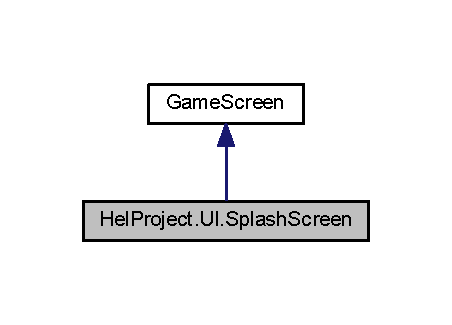
\includegraphics[width=217pt]{class_hel_project_1_1_u_i_1_1_splash_screen__inherit__graph}
\end{center}
\end{figure}


Collaboration diagram for Hel\+Project.\+U\+I.\+Splash\+Screen\+:\nopagebreak
\begin{figure}[H]
\begin{center}
\leavevmode
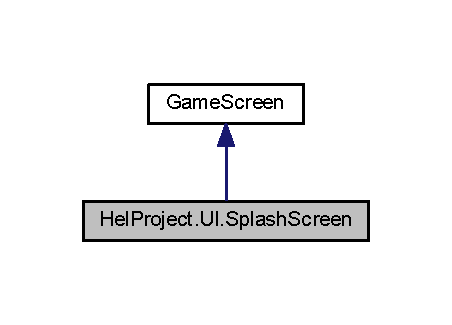
\includegraphics[width=217pt]{class_hel_project_1_1_u_i_1_1_splash_screen__coll__graph}
\end{center}
\end{figure}
\subsection*{Public Member Functions}
\begin{DoxyCompactItemize}
\item 
override void \hyperlink{class_hel_project_1_1_u_i_1_1_splash_screen_a5a20d77a817cf6982efb89576d5e32d0}{Load\+Content} ()
\begin{DoxyCompactList}\small\item\em Loads the content of the screen \end{DoxyCompactList}\item 
override void \hyperlink{class_hel_project_1_1_u_i_1_1_splash_screen_ad00f04421eabaf7b516eddc371350ef2}{Unload\+Content} ()
\begin{DoxyCompactList}\small\item\em Unloads the content of the screen \end{DoxyCompactList}\item 
override void \hyperlink{class_hel_project_1_1_u_i_1_1_splash_screen_abf282bea4e6f1ee8a6ab03f812f130d3}{Update} (Game\+Time game\+Time)
\begin{DoxyCompactList}\small\item\em Updates the content screen \end{DoxyCompactList}\item 
override void \hyperlink{class_hel_project_1_1_u_i_1_1_splash_screen_a5c978af3192a5de1f344e8b16821a2d8}{Draw} (Sprite\+Batch sprite\+Batch)
\begin{DoxyCompactList}\small\item\em Draws the content of the screen \end{DoxyCompactList}\end{DoxyCompactItemize}
\subsection*{Properties}
\begin{DoxyCompactItemize}
\item 
\hyperlink{class_hel_project_1_1_u_i_1_1_game_screen}{Game\+Screen} \hyperlink{class_hel_project_1_1_u_i_1_1_splash_screen_abcc41435703b36b419b18600a05a42f5}{Next\+Screen}\hspace{0.3cm}{\ttfamily  \mbox{[}get, set\mbox{]}}
\begin{DoxyCompactList}\small\item\em Next screen after the splash screen \end{DoxyCompactList}\item 
\hyperlink{class_hel_project_1_1_u_i_1_1_image}{Image} \hyperlink{class_hel_project_1_1_u_i_1_1_splash_screen_adb2597647fe28bc0a62aec62c5a4e435}{Background\+Image}\hspace{0.3cm}{\ttfamily  \mbox{[}get, set\mbox{]}}
\begin{DoxyCompactList}\small\item\em Background \hyperlink{class_hel_project_1_1_u_i_1_1_image}{Image} of the splashscreen \end{DoxyCompactList}\end{DoxyCompactItemize}


\subsection{Detailed Description}
Splash screen 



\subsection{Member Function Documentation}
\hypertarget{class_hel_project_1_1_u_i_1_1_splash_screen_a5c978af3192a5de1f344e8b16821a2d8}{}\index{Hel\+Project\+::\+U\+I\+::\+Splash\+Screen@{Hel\+Project\+::\+U\+I\+::\+Splash\+Screen}!Draw@{Draw}}
\index{Draw@{Draw}!Hel\+Project\+::\+U\+I\+::\+Splash\+Screen@{Hel\+Project\+::\+U\+I\+::\+Splash\+Screen}}
\subsubsection[{Draw}]{\setlength{\rightskip}{0pt plus 5cm}override void Hel\+Project.\+U\+I.\+Splash\+Screen.\+Draw (
\begin{DoxyParamCaption}
\item[{Sprite\+Batch}]{sprite\+Batch}
\end{DoxyParamCaption}
)\hspace{0.3cm}{\ttfamily [virtual]}}\label{class_hel_project_1_1_u_i_1_1_splash_screen_a5c978af3192a5de1f344e8b16821a2d8}


Draws the content of the screen 


\begin{DoxyParams}{Parameters}
{\em sprite\+Batch} & \\
\hline
\end{DoxyParams}


Reimplemented from \hyperlink{class_hel_project_1_1_u_i_1_1_game_screen_ace6f51c0a6c5206a5c58cefd0eba2797}{Hel\+Project.\+U\+I.\+Game\+Screen}.

\hypertarget{class_hel_project_1_1_u_i_1_1_splash_screen_a5a20d77a817cf6982efb89576d5e32d0}{}\index{Hel\+Project\+::\+U\+I\+::\+Splash\+Screen@{Hel\+Project\+::\+U\+I\+::\+Splash\+Screen}!Load\+Content@{Load\+Content}}
\index{Load\+Content@{Load\+Content}!Hel\+Project\+::\+U\+I\+::\+Splash\+Screen@{Hel\+Project\+::\+U\+I\+::\+Splash\+Screen}}
\subsubsection[{Load\+Content}]{\setlength{\rightskip}{0pt plus 5cm}override void Hel\+Project.\+U\+I.\+Splash\+Screen.\+Load\+Content (
\begin{DoxyParamCaption}
{}
\end{DoxyParamCaption}
)\hspace{0.3cm}{\ttfamily [virtual]}}\label{class_hel_project_1_1_u_i_1_1_splash_screen_a5a20d77a817cf6982efb89576d5e32d0}


Loads the content of the screen 



Reimplemented from \hyperlink{class_hel_project_1_1_u_i_1_1_game_screen_aa4e15890ede3b8da390ffe0cecff3703}{Hel\+Project.\+U\+I.\+Game\+Screen}.

\hypertarget{class_hel_project_1_1_u_i_1_1_splash_screen_ad00f04421eabaf7b516eddc371350ef2}{}\index{Hel\+Project\+::\+U\+I\+::\+Splash\+Screen@{Hel\+Project\+::\+U\+I\+::\+Splash\+Screen}!Unload\+Content@{Unload\+Content}}
\index{Unload\+Content@{Unload\+Content}!Hel\+Project\+::\+U\+I\+::\+Splash\+Screen@{Hel\+Project\+::\+U\+I\+::\+Splash\+Screen}}
\subsubsection[{Unload\+Content}]{\setlength{\rightskip}{0pt plus 5cm}override void Hel\+Project.\+U\+I.\+Splash\+Screen.\+Unload\+Content (
\begin{DoxyParamCaption}
{}
\end{DoxyParamCaption}
)\hspace{0.3cm}{\ttfamily [virtual]}}\label{class_hel_project_1_1_u_i_1_1_splash_screen_ad00f04421eabaf7b516eddc371350ef2}


Unloads the content of the screen 



Reimplemented from \hyperlink{class_hel_project_1_1_u_i_1_1_game_screen_a97560de3aeb8b283fca89c1682ec778f}{Hel\+Project.\+U\+I.\+Game\+Screen}.

\hypertarget{class_hel_project_1_1_u_i_1_1_splash_screen_abf282bea4e6f1ee8a6ab03f812f130d3}{}\index{Hel\+Project\+::\+U\+I\+::\+Splash\+Screen@{Hel\+Project\+::\+U\+I\+::\+Splash\+Screen}!Update@{Update}}
\index{Update@{Update}!Hel\+Project\+::\+U\+I\+::\+Splash\+Screen@{Hel\+Project\+::\+U\+I\+::\+Splash\+Screen}}
\subsubsection[{Update}]{\setlength{\rightskip}{0pt plus 5cm}override void Hel\+Project.\+U\+I.\+Splash\+Screen.\+Update (
\begin{DoxyParamCaption}
\item[{Game\+Time}]{game\+Time}
\end{DoxyParamCaption}
)\hspace{0.3cm}{\ttfamily [virtual]}}\label{class_hel_project_1_1_u_i_1_1_splash_screen_abf282bea4e6f1ee8a6ab03f812f130d3}


Updates the content screen 


\begin{DoxyParams}{Parameters}
{\em game\+Time} & \\
\hline
\end{DoxyParams}


Reimplemented from \hyperlink{class_hel_project_1_1_u_i_1_1_game_screen_a4aefe31814b0081be3ba4f1243b8cee6}{Hel\+Project.\+U\+I.\+Game\+Screen}.



\subsection{Property Documentation}
\hypertarget{class_hel_project_1_1_u_i_1_1_splash_screen_adb2597647fe28bc0a62aec62c5a4e435}{}\index{Hel\+Project\+::\+U\+I\+::\+Splash\+Screen@{Hel\+Project\+::\+U\+I\+::\+Splash\+Screen}!Background\+Image@{Background\+Image}}
\index{Background\+Image@{Background\+Image}!Hel\+Project\+::\+U\+I\+::\+Splash\+Screen@{Hel\+Project\+::\+U\+I\+::\+Splash\+Screen}}
\subsubsection[{Background\+Image}]{\setlength{\rightskip}{0pt plus 5cm}{\bf Image} Hel\+Project.\+U\+I.\+Splash\+Screen.\+Background\+Image\hspace{0.3cm}{\ttfamily [get]}, {\ttfamily [set]}}\label{class_hel_project_1_1_u_i_1_1_splash_screen_adb2597647fe28bc0a62aec62c5a4e435}


Background \hyperlink{class_hel_project_1_1_u_i_1_1_image}{Image} of the splashscreen 

\hypertarget{class_hel_project_1_1_u_i_1_1_splash_screen_abcc41435703b36b419b18600a05a42f5}{}\index{Hel\+Project\+::\+U\+I\+::\+Splash\+Screen@{Hel\+Project\+::\+U\+I\+::\+Splash\+Screen}!Next\+Screen@{Next\+Screen}}
\index{Next\+Screen@{Next\+Screen}!Hel\+Project\+::\+U\+I\+::\+Splash\+Screen@{Hel\+Project\+::\+U\+I\+::\+Splash\+Screen}}
\subsubsection[{Next\+Screen}]{\setlength{\rightskip}{0pt plus 5cm}{\bf Game\+Screen} Hel\+Project.\+U\+I.\+Splash\+Screen.\+Next\+Screen\hspace{0.3cm}{\ttfamily [get]}, {\ttfamily [set]}}\label{class_hel_project_1_1_u_i_1_1_splash_screen_abcc41435703b36b419b18600a05a42f5}


Next screen after the splash screen 



The documentation for this class was generated from the following file\+:\begin{DoxyCompactItemize}
\item 
src/\+Hel\+Project/\+U\+I/Splash\+Screen.\+cs\end{DoxyCompactItemize}

\hypertarget{class_hel_project_1_1_u_i_1_1_temporary_dictionnary_item}{}\section{Hel\+Project.\+U\+I.\+Temporary\+Dictionnary\+Item Class Reference}
\label{class_hel_project_1_1_u_i_1_1_temporary_dictionnary_item}\index{Hel\+Project.\+U\+I.\+Temporary\+Dictionnary\+Item@{Hel\+Project.\+U\+I.\+Temporary\+Dictionnary\+Item}}


Class used for the serialization/deserialization of the \hyperlink{class_hel_project_1_1_u_i_1_1_texture_manager}{Texture\+Manager} class  


\subsection*{Public Attributes}
\begin{DoxyCompactItemize}
\item 
\hypertarget{class_hel_project_1_1_u_i_1_1_temporary_dictionnary_item_a43f95cb22933c364f57dbf519248eb91}{}string {\bfseries id}\label{class_hel_project_1_1_u_i_1_1_temporary_dictionnary_item_a43f95cb22933c364f57dbf519248eb91}

\item 
\hypertarget{class_hel_project_1_1_u_i_1_1_temporary_dictionnary_item_a7ce5be50ae172de4a0dc1312766e6dfc}{}string {\bfseries path}\label{class_hel_project_1_1_u_i_1_1_temporary_dictionnary_item_a7ce5be50ae172de4a0dc1312766e6dfc}

\end{DoxyCompactItemize}


\subsection{Detailed Description}
Class used for the serialization/deserialization of the \hyperlink{class_hel_project_1_1_u_i_1_1_texture_manager}{Texture\+Manager} class 



The documentation for this class was generated from the following file\+:\begin{DoxyCompactItemize}
\item 
src/\+Hel\+Project/\+U\+I/Texture\+Manager.\+cs\end{DoxyCompactItemize}

\hypertarget{class_hel_project_1_1_u_i_1_1_texture_manager}{}\section{Hel\+Project.\+U\+I.\+Texture\+Manager Class Reference}
\label{class_hel_project_1_1_u_i_1_1_texture_manager}\index{Hel\+Project.\+U\+I.\+Texture\+Manager@{Hel\+Project.\+U\+I.\+Texture\+Manager}}


Gets all the textures  


\subsection*{Public Member Functions}
\begin{DoxyCompactItemize}
\item 
void \hyperlink{class_hel_project_1_1_u_i_1_1_texture_manager_ada156bc3a5f02b869a558d3ed2fd73c2}{Load} (string path)
\begin{DoxyCompactList}\small\item\em Loads all the textures paths from the given file \end{DoxyCompactList}\item 
void \hyperlink{class_hel_project_1_1_u_i_1_1_texture_manager_af20f01be3ff211887c33209abdeb72e5}{Save} (string path)
\begin{DoxyCompactList}\small\item\em Save all the textures paths to the given location \end{DoxyCompactList}\end{DoxyCompactItemize}
\subsection*{Properties}
\begin{DoxyCompactItemize}
\item 
I\+Dictionary$<$ string, string $>$ \hyperlink{class_hel_project_1_1_u_i_1_1_texture_manager_a0524c77f2c5fd5c6f3eb57645bf8a521}{Textures\+Paths}\hspace{0.3cm}{\ttfamily  \mbox{[}get, set\mbox{]}}
\begin{DoxyCompactList}\small\item\em Path of all the textures \end{DoxyCompactList}\item 
I\+Dictionary$<$ string, Texture2\+D $>$ \hyperlink{class_hel_project_1_1_u_i_1_1_texture_manager_a57751418291b635f8c1f16f8ef9a1468}{Loaded\+Textures}\hspace{0.3cm}{\ttfamily  \mbox{[}get, set\mbox{]}}
\begin{DoxyCompactList}\small\item\em Loaded textures \end{DoxyCompactList}\item 
static \hyperlink{class_hel_project_1_1_u_i_1_1_texture_manager}{Texture\+Manager} \hyperlink{class_hel_project_1_1_u_i_1_1_texture_manager_a583c9e38fd71caf9d6b1cf4a1543ca0a}{Instance}\hspace{0.3cm}{\ttfamily  \mbox{[}get\mbox{]}}
\begin{DoxyCompactList}\small\item\em Instance of the class \end{DoxyCompactList}\end{DoxyCompactItemize}


\subsection{Detailed Description}
Gets all the textures 



\subsection{Member Function Documentation}
\hypertarget{class_hel_project_1_1_u_i_1_1_texture_manager_ada156bc3a5f02b869a558d3ed2fd73c2}{}\index{Hel\+Project\+::\+U\+I\+::\+Texture\+Manager@{Hel\+Project\+::\+U\+I\+::\+Texture\+Manager}!Load@{Load}}
\index{Load@{Load}!Hel\+Project\+::\+U\+I\+::\+Texture\+Manager@{Hel\+Project\+::\+U\+I\+::\+Texture\+Manager}}
\subsubsection[{Load}]{\setlength{\rightskip}{0pt plus 5cm}void Hel\+Project.\+U\+I.\+Texture\+Manager.\+Load (
\begin{DoxyParamCaption}
\item[{string}]{path}
\end{DoxyParamCaption}
)}\label{class_hel_project_1_1_u_i_1_1_texture_manager_ada156bc3a5f02b869a558d3ed2fd73c2}


Loads all the textures paths from the given file 


\begin{DoxyParams}{Parameters}
{\em path} & Path of the initialization file (.xml)\\
\hline
\end{DoxyParams}
\hypertarget{class_hel_project_1_1_u_i_1_1_texture_manager_af20f01be3ff211887c33209abdeb72e5}{}\index{Hel\+Project\+::\+U\+I\+::\+Texture\+Manager@{Hel\+Project\+::\+U\+I\+::\+Texture\+Manager}!Save@{Save}}
\index{Save@{Save}!Hel\+Project\+::\+U\+I\+::\+Texture\+Manager@{Hel\+Project\+::\+U\+I\+::\+Texture\+Manager}}
\subsubsection[{Save}]{\setlength{\rightskip}{0pt plus 5cm}void Hel\+Project.\+U\+I.\+Texture\+Manager.\+Save (
\begin{DoxyParamCaption}
\item[{string}]{path}
\end{DoxyParamCaption}
)}\label{class_hel_project_1_1_u_i_1_1_texture_manager_af20f01be3ff211887c33209abdeb72e5}


Save all the textures paths to the given location 


\begin{DoxyParams}{Parameters}
{\em path} & Path of the location/file\\
\hline
\end{DoxyParams}


\subsection{Property Documentation}
\hypertarget{class_hel_project_1_1_u_i_1_1_texture_manager_a583c9e38fd71caf9d6b1cf4a1543ca0a}{}\index{Hel\+Project\+::\+U\+I\+::\+Texture\+Manager@{Hel\+Project\+::\+U\+I\+::\+Texture\+Manager}!Instance@{Instance}}
\index{Instance@{Instance}!Hel\+Project\+::\+U\+I\+::\+Texture\+Manager@{Hel\+Project\+::\+U\+I\+::\+Texture\+Manager}}
\subsubsection[{Instance}]{\setlength{\rightskip}{0pt plus 5cm}{\bf Texture\+Manager} Hel\+Project.\+U\+I.\+Texture\+Manager.\+Instance\hspace{0.3cm}{\ttfamily [static]}, {\ttfamily [get]}}\label{class_hel_project_1_1_u_i_1_1_texture_manager_a583c9e38fd71caf9d6b1cf4a1543ca0a}


Instance of the class 

\hypertarget{class_hel_project_1_1_u_i_1_1_texture_manager_a57751418291b635f8c1f16f8ef9a1468}{}\index{Hel\+Project\+::\+U\+I\+::\+Texture\+Manager@{Hel\+Project\+::\+U\+I\+::\+Texture\+Manager}!Loaded\+Textures@{Loaded\+Textures}}
\index{Loaded\+Textures@{Loaded\+Textures}!Hel\+Project\+::\+U\+I\+::\+Texture\+Manager@{Hel\+Project\+::\+U\+I\+::\+Texture\+Manager}}
\subsubsection[{Loaded\+Textures}]{\setlength{\rightskip}{0pt plus 5cm}I\+Dictionary$<$string, Texture2\+D$>$ Hel\+Project.\+U\+I.\+Texture\+Manager.\+Loaded\+Textures\hspace{0.3cm}{\ttfamily [get]}, {\ttfamily [set]}}\label{class_hel_project_1_1_u_i_1_1_texture_manager_a57751418291b635f8c1f16f8ef9a1468}


Loaded textures 

\hypertarget{class_hel_project_1_1_u_i_1_1_texture_manager_a0524c77f2c5fd5c6f3eb57645bf8a521}{}\index{Hel\+Project\+::\+U\+I\+::\+Texture\+Manager@{Hel\+Project\+::\+U\+I\+::\+Texture\+Manager}!Textures\+Paths@{Textures\+Paths}}
\index{Textures\+Paths@{Textures\+Paths}!Hel\+Project\+::\+U\+I\+::\+Texture\+Manager@{Hel\+Project\+::\+U\+I\+::\+Texture\+Manager}}
\subsubsection[{Textures\+Paths}]{\setlength{\rightskip}{0pt plus 5cm}I\+Dictionary$<$string, string$>$ Hel\+Project.\+U\+I.\+Texture\+Manager.\+Textures\+Paths\hspace{0.3cm}{\ttfamily [get]}, {\ttfamily [set]}}\label{class_hel_project_1_1_u_i_1_1_texture_manager_a0524c77f2c5fd5c6f3eb57645bf8a521}


Path of all the textures 

key = name of the texture value = path to texture 

The documentation for this class was generated from the following file\+:\begin{DoxyCompactItemize}
\item 
src/\+Hel\+Project/\+U\+I/Texture\+Manager.\+cs\end{DoxyCompactItemize}

\hypertarget{class_hel_project_1_1_tools_1_1_xml_manager}{}\section{Hel\+Project.\+Tools.\+Xml\+Manager$<$ T $>$ Class Template Reference}
\label{class_hel_project_1_1_tools_1_1_xml_manager}\index{Hel\+Project.\+Tools.\+Xml\+Manager$<$ T $>$@{Hel\+Project.\+Tools.\+Xml\+Manager$<$ T $>$}}
\subsection*{Public Member Functions}
\begin{DoxyCompactItemize}
\item 
T \hyperlink{class_hel_project_1_1_tools_1_1_xml_manager_aaa77414aaedc8de70b8033fcbc776e20}{Load} (string path)
\begin{DoxyCompactList}\small\item\em Loads a X\+M\+L \end{DoxyCompactList}\item 
void \hyperlink{class_hel_project_1_1_tools_1_1_xml_manager_abe9006549ede6ee536ec111b75d17eae}{Save} (string path, object obj)
\begin{DoxyCompactList}\small\item\em Saves an X\+M\+L \end{DoxyCompactList}\end{DoxyCompactItemize}
\subsection*{Properties}
\begin{DoxyCompactItemize}
\item 
Type \hyperlink{class_hel_project_1_1_tools_1_1_xml_manager_a4c29b7a37cf80588e6bc8a45626262a5}{Type\+Class}\hspace{0.3cm}{\ttfamily  \mbox{[}get, set\mbox{]}}
\begin{DoxyCompactList}\small\item\em Type of the class that the \hyperlink{class_hel_project_1_1_tools_1_1_xml_manager}{Xml\+Manager} represents \end{DoxyCompactList}\end{DoxyCompactItemize}


\subsection{Member Function Documentation}
\hypertarget{class_hel_project_1_1_tools_1_1_xml_manager_aaa77414aaedc8de70b8033fcbc776e20}{}\index{Hel\+Project\+::\+Tools\+::\+Xml\+Manager@{Hel\+Project\+::\+Tools\+::\+Xml\+Manager}!Load@{Load}}
\index{Load@{Load}!Hel\+Project\+::\+Tools\+::\+Xml\+Manager@{Hel\+Project\+::\+Tools\+::\+Xml\+Manager}}
\subsubsection[{Load}]{\setlength{\rightskip}{0pt plus 5cm}T {\bf Hel\+Project.\+Tools.\+Xml\+Manager}$<$ T $>$.Load (
\begin{DoxyParamCaption}
\item[{string}]{path}
\end{DoxyParamCaption}
)}\label{class_hel_project_1_1_tools_1_1_xml_manager_aaa77414aaedc8de70b8033fcbc776e20}


Loads a X\+M\+L 


\begin{DoxyParams}{Parameters}
{\em path} & path of the xml\\
\hline
\end{DoxyParams}
\begin{DoxyReturn}{Returns}
Object of the xml
\end{DoxyReturn}
\hypertarget{class_hel_project_1_1_tools_1_1_xml_manager_abe9006549ede6ee536ec111b75d17eae}{}\index{Hel\+Project\+::\+Tools\+::\+Xml\+Manager@{Hel\+Project\+::\+Tools\+::\+Xml\+Manager}!Save@{Save}}
\index{Save@{Save}!Hel\+Project\+::\+Tools\+::\+Xml\+Manager@{Hel\+Project\+::\+Tools\+::\+Xml\+Manager}}
\subsubsection[{Save}]{\setlength{\rightskip}{0pt plus 5cm}void {\bf Hel\+Project.\+Tools.\+Xml\+Manager}$<$ T $>$.Save (
\begin{DoxyParamCaption}
\item[{string}]{path, }
\item[{object}]{obj}
\end{DoxyParamCaption}
)}\label{class_hel_project_1_1_tools_1_1_xml_manager_abe9006549ede6ee536ec111b75d17eae}


Saves an X\+M\+L 


\begin{DoxyParams}{Parameters}
{\em path} & path of the xml file\\
\hline
{\em obj} & object to serialize\\
\hline
\end{DoxyParams}


\subsection{Property Documentation}
\hypertarget{class_hel_project_1_1_tools_1_1_xml_manager_a4c29b7a37cf80588e6bc8a45626262a5}{}\index{Hel\+Project\+::\+Tools\+::\+Xml\+Manager@{Hel\+Project\+::\+Tools\+::\+Xml\+Manager}!Type\+Class@{Type\+Class}}
\index{Type\+Class@{Type\+Class}!Hel\+Project\+::\+Tools\+::\+Xml\+Manager@{Hel\+Project\+::\+Tools\+::\+Xml\+Manager}}
\subsubsection[{Type\+Class}]{\setlength{\rightskip}{0pt plus 5cm}Type {\bf Hel\+Project.\+Tools.\+Xml\+Manager}$<$ T $>$.Type\+Class\hspace{0.3cm}{\ttfamily [get]}, {\ttfamily [set]}}\label{class_hel_project_1_1_tools_1_1_xml_manager_a4c29b7a37cf80588e6bc8a45626262a5}


Type of the class that the \hyperlink{class_hel_project_1_1_tools_1_1_xml_manager}{Xml\+Manager} represents 



The documentation for this class was generated from the following file\+:\begin{DoxyCompactItemize}
\item 
src/\+Hel\+Project/\+Tools/Xml\+Manager.\+cs\end{DoxyCompactItemize}

%--- End generated contents ---

% Index
\backmatter
\newpage
\phantomsection
\clearemptydoublepage
\addcontentsline{toc}{chapter}{Index}
\printindex

\end{document}
